%%%%%%%%%%%%%%%%%%%%%%%%%%%%%%%%%%%%%%%%%
%  My documentation report
%  Objetive: Explain what I did and how, so someone can continue with the investigation
%
% Important note:
% Chapter heading images should have a 2:1 width:height ratio,
% e.g. 920px width and 460px height.
%
%%%%%%%%%%%%%%%%%%%%%%%%%%%%%%%%%%%%%%%%%

%----------------------------------------------------------------------------------------
% PACKAGES AND OTHER DOCUMENT CONFIGURATIONS
%----------------------------------------------------------------------------------------

\documentclass[11pt]{book} % Default font size and left-justified equations
\usepackage[top=3cm,bottom=3cm,left=3.2cm,right=3.2cm,headsep=10pt,letterpaper]{geometry} % Page margins
\usepackage{xcolor} % Required for specifying colors by name
\definecolor{ocre}{RGB}{52,177,201} % Define the orange color used for highlighting throughout the book

%%%%%%%%%%%%%%%%%%%%%%%%%%%%%%%%%%%%%%%%%
% The Legrand Orange Book
% Structural Definitions File
% Version 2.0 (9/2/15)
%
% Original author:
% Mathias Legrand (legrand.mathias@gmail.com) with modifications by:
% Vel (vel@latextemplates.com)
% 
% This file has been downloaded from:
% http://www.LaTeXTemplates.com
%
% License:
% CC BY-NC-SA 3.0 (http://creativecommons.org/licenses/by-nc-sa/3.0/)
%
%%%%%%%%%%%%%%%%%%%%%%%%%%%%%%%%%%%%%%%%%

%----------------------------------------------------------------------------------------
%	VARIOUS REQUIRED PACKAGES AND CONFIGURATIONS
%----------------------------------------------------------------------------------------

\usepackage[top=3cm,bottom=3cm,left=3cm,right=3cm,headsep=10pt,a4paper]{geometry} % Page margins

\usepackage{graphicx} % Required for including pictures
\graphicspath{{Pictures/}} % Specifies the directory where pictures are stored

\usepackage{lipsum} % Inserts dummy text

\usepackage{tikz} % Required for drawing custom shapes

\usepackage[english]{babel} % English language/hyphenation

\usepackage{enumitem} % Customize lists
\setlist{nolistsep} % Reduce spacing between bullet points and numbered lists

\usepackage{booktabs} % Required for nicer horizontal rules in tables

\usepackage{xcolor} % Required for specifying colors by name
% \definecolor{ocre}{RGB}{243,102,25} % Orange
% \definecolor{ocre}{RGB}{0,0,128} % Navy
% \definecolor{ocre}{RGB}{65,105,225} % Royal Blue
\definecolor{ocre}{RGB}{255,69,0} % Orange Red

%----------------------------------------------------------------------------------------
%	FONTS
%----------------------------------------------------------------------------------------

% \usepackage{avant} % Use the Avantgarde font for headings
% \usepackage{times} % Use the Times font for headings
% \usepackage{mathptmx} % Use the Adobe Times Roman as the default text font together with math symbols from the Sym­bol, Chancery and Com­puter Modern fonts
\usepackage{libertine}
\usepackage{tgcursor}

\usepackage{microtype} % Slightly tweak font spacing for aesthetics
\usepackage[utf8]{inputenc} % Required for including letters with accents
\usepackage[T1]{fontenc} % Use 8-bit encoding that has 256 glyphs

%----------------------------------------------------------------------------------------
%	BIBLIOGRAPHY
%----------------------------------------------------------------------------------------

% \usepackage[style=alphabetic,citestyle=numeric,sorting=nyt,sortcites=true,autopunct=true,babel=hyphen,hyperref=true,abbreviate=false,backref=true,backend=biber]{biblatex}
% \usepackage{biblatex}
% \addbibresource{allrefs.bib} % BibTeX bibliography file
% \defbibheading{bibempty}{}

\usepackage{calc} % For simpler calculation - used for spacing the index letter headings correctly

%----------------------------------------------------------------------------------------
%	MAIN TABLE OF CONTENTS
%----------------------------------------------------------------------------------------

\usepackage{titletoc} % Required for manipulating the table of contents

\contentsmargin{0cm} % Removes the default margin

% Part text styling
\titlecontents{part}[0cm]
{\addvspace{20pt}\centering\large\bfseries}
{}
{}
{}

% Chapter text styling
\titlecontents{chapter}[1.25cm] % Indentation
{\addvspace{12pt}\large\sffamily\bfseries} % Spacing and font options for chapters
{\color{ocre!60}\contentslabel[\Large\thecontentslabel]{1.25cm}\color{ocre}} % Chapter number
{\color{ocre}}  
{\color{ocre!60}\normalsize\;\titlerule*[.5pc]{.}\;\thecontentspage} % Page number

% Section text styling
\titlecontents{section}[1.25cm] % Indentation
{\addvspace{3pt}\sffamily\bfseries} % Spacing and font options for sections
{\contentslabel[\thecontentslabel]{1.25cm}} % Section number
{}
{\hfill\color{black}\thecontentspage} % Page number
[]

% Subsection text styling
\titlecontents{subsection}[1.25cm] % Indentation
{\addvspace{1pt}\sffamily\small} % Spacing and font options for subsections
{\contentslabel[\thecontentslabel]{1.25cm}} % Subsection number
{}
{\ \titlerule*[.5pc]{.}\;\thecontentspage} % Page number
[]

% List of figures
\titlecontents{figure}[0em]
{\addvspace{-5pt}\sffamily}
{\thecontentslabel\hspace*{1em}}
{}
{\ \titlerule*[.5pc]{.}\;\thecontentspage}
[]

% List of tables
\titlecontents{table}[0em]
{\addvspace{-5pt}\sffamily}
{\thecontentslabel\hspace*{1em}}
{}
{\ \titlerule*[.5pc]{.}\;\thecontentspage}
[]

%----------------------------------------------------------------------------------------
%	MINI TABLE OF CONTENTS IN PART HEADS
%----------------------------------------------------------------------------------------

% Chapter text styling
\titlecontents{lchapter}[0em] % Indenting
{\addvspace{15pt}\large\sffamily\bfseries} % Spacing and font options for chapters
{\color{ocre}\contentslabel[\Large\thecontentslabel]{1.25cm}\color{ocre}} % Chapter number
{}  
{\color{ocre}\normalsize\sffamily\bfseries\;\titlerule*[.5pc]{.}\;\thecontentspage} % Page number

% Section text styling
\titlecontents{lsection}[0em] % Indenting
{\sffamily\small} % Spacing and font options for sections
{\contentslabel[\thecontentslabel]{1.25cm}} % Section number
{}
{}

% Subsection text styling
\titlecontents{lsubsection}[.5em] % Indentation
{\normalfont\footnotesize\sffamily} % Font settings
{}
{}
{}

%----------------------------------------------------------------------------------------
%	PAGE HEADERS
%----------------------------------------------------------------------------------------

\usepackage{fancyhdr} % Required for header and footer configuration

\pagestyle{fancy}
\renewcommand{\chaptermark}[1]{\markboth{\sffamily\normalsize\bfseries\chaptername\ \thechapter.\ #1}{}} % Chapter text font settings
\renewcommand{\sectionmark}[1]{\markright{\sffamily\normalsize\thesection\hspace{5pt}#1}{}} % Section text font settings
\fancyhf{} \fancyhead[LE,RO]{\sffamily\normalsize\thepage} % Font setting for the page number in the header
\fancyhead[LO]{\rightmark} % Print the nearest section name on the left side of odd pages
\fancyhead[RE]{\leftmark} % Print the current chapter name on the right side of even pages
\renewcommand{\headrulewidth}{0.5pt} % Width of the rule under the header
\addtolength{\headheight}{2.5pt} % Increase the spacing around the header slightly
\renewcommand{\footrulewidth}{0pt} % Removes the rule in the footer
\fancypagestyle{plain}{\fancyhead{}\renewcommand{\headrulewidth}{0pt}} % Style for when a plain pagestyle is specified

% Removes the header from odd empty pages at the end of chapters
\makeatletter
\renewcommand{\cleardoublepage}{
\clearpage\ifodd\c@page\else
\hbox{}
\vspace*{\fill}
\thispagestyle{empty}
\newpage
\fi}

%----------------------------------------------------------------------------------------
%	THEOREM STYLES
%----------------------------------------------------------------------------------------

\usepackage{amsmath,amsfonts,amssymb,amsthm} % For math equations, theorems, symbols, etc

\newcommand{\intoo}[2]{\mathopen{]}#1\,;#2\mathclose{[}}
\newcommand{\ud}{\mathop{\mathrm{{}d}}\mathopen{}}
\newcommand{\intff}[2]{\mathopen{[}#1\,;#2\mathclose{]}}
\newtheorem{notation}{Notation}[chapter]

% Boxed/framed environments
\newtheoremstyle{ocrenumbox}% % Theorem style name
{0pt}% Space above
{0pt}% Space below
{\normalfont}% % Body font
{}% Indent amount
{\small\bf\sffamily\color{ocre}}% % Theorem head font
{\;}% Punctuation after theorem head
{0.25em}% Space after theorem head
{\small\sffamily\color{ocre}\thmname{#1}\nobreakspace\thmnumber{\@ifnotempty{#1}{}\@upn{#2}}% Theorem text (e.g. Theorem 2.1)
\thmnote{\nobreakspace\the\thm@notefont\sffamily\bfseries\color{black}---\nobreakspace#3.}} % Optional theorem note
\renewcommand{\qedsymbol}{$\blacksquare$}% Optional qed square

\newtheoremstyle{blacknumex}% Theorem style name
{5pt}% Space above
{5pt}% Space below
{\normalfont}% Body font
{} % Indent amount
{\small\bf\sffamily}% Theorem head font
{\;}% Punctuation after theorem head
{0.25em}% Space after theorem head
{\small\sffamily{\tiny\ensuremath{\blacksquare}}\nobreakspace\thmname{#1}\nobreakspace\thmnumber{\@ifnotempty{#1}{}\@upn{#2}}% Theorem text (e.g. Theorem 2.1)
\thmnote{\nobreakspace\the\thm@notefont\sffamily\bfseries---\nobreakspace#3.}}% Optional theorem note

\newtheoremstyle{blacknumbox} % Theorem style name
{0pt}% Space above
{0pt}% Space below
{\normalfont}% Body font
{}% Indent amount
{\small\bf\sffamily}% Theorem head font
{\;}% Punctuation after theorem head
{0.25em}% Space after theorem head
{\small\sffamily\thmname{#1}\nobreakspace\thmnumber{\@ifnotempty{#1}{}\@upn{#2}}% Theorem text (e.g. Theorem 2.1)
\thmnote{\nobreakspace\the\thm@notefont\sffamily\bfseries---\nobreakspace#3.}}% Optional theorem note

% Non-boxed/non-framed environments
\newtheoremstyle{ocrenum}% % Theorem style name
{5pt}% Space above
{5pt}% Space below
{\normalfont}% % Body font
{}% Indent amount
{\small\bf\sffamily\color{ocre}}% % Theorem head font
{\;}% Punctuation after theorem head
{0.25em}% Space after theorem head
{\small\sffamily\color{ocre}\thmname{#1}\nobreakspace\thmnumber{\@ifnotempty{#1}{}\@upn{#2}}% Theorem text (e.g. Theorem 2.1)
\thmnote{\nobreakspace\the\thm@notefont\sffamily\bfseries\color{black}---\nobreakspace#3.}} % Optional theorem note
\renewcommand{\qedsymbol}{$\blacksquare$}% Optional qed square
\makeatother

% Defines the theorem text style for each type of theorem to one of the three styles above
\newcounter{dummy} 
\numberwithin{dummy}{section}
\theoremstyle{ocrenumbox}
\newtheorem{theoremeT}[dummy]{Theorem}
\newtheorem{problem}{Problem}[chapter]
\newtheorem{exerciseT}{Exercise}[chapter]
\theoremstyle{blacknumex}
\newtheorem{exampleT}{Example}[chapter]
\theoremstyle{blacknumbox}
\newtheorem{vocabulary}{Vocabulary}[chapter]
\newtheorem{definitionT}{Definition}[section]
\newtheorem{corollaryT}[dummy]{Corollary}
\theoremstyle{ocrenum}
\newtheorem{proposition}[dummy]{Proposition}

%----------------------------------------------------------------------------------------
%	DEFINITION OF COLORED BOXES
%----------------------------------------------------------------------------------------

\RequirePackage[framemethod=default]{mdframed} % Required for creating the theorem, definition, exercise and corollary boxes

% Theorem box
\newmdenv[skipabove=7pt,
skipbelow=7pt,
backgroundcolor=black!5,
linecolor=ocre,
innerleftmargin=5pt,
innerrightmargin=5pt,
innertopmargin=5pt,
leftmargin=0cm,
rightmargin=0cm,
innerbottommargin=5pt]{tBox}

% Exercise box	  
\newmdenv[skipabove=7pt,
skipbelow=7pt,
rightline=false,
leftline=true,
topline=false,
bottomline=false,
backgroundcolor=ocre!10,
linecolor=ocre,
innerleftmargin=5pt,
innerrightmargin=5pt,
innertopmargin=5pt,
innerbottommargin=5pt,
leftmargin=0cm,
rightmargin=0cm,
linewidth=4pt]{eBox}	

% Definition box
\newmdenv[skipabove=7pt,
skipbelow=7pt,
rightline=false,
leftline=true,
topline=false,
bottomline=false,
linecolor=ocre,
innerleftmargin=5pt,
innerrightmargin=5pt,
innertopmargin=0pt,
leftmargin=0cm,
rightmargin=0cm,
linewidth=4pt,
innerbottommargin=0pt]{dBox}	

% Corollary box
\newmdenv[skipabove=7pt,
skipbelow=7pt,
rightline=false,
leftline=true,
topline=false,
bottomline=false,
linecolor=gray,
backgroundcolor=black!5,
innerleftmargin=5pt,
innerrightmargin=5pt,
innertopmargin=5pt,
leftmargin=0cm,
rightmargin=0cm,
linewidth=4pt,
innerbottommargin=5pt]{cBox}

% Creates an environment for each type of theorem and assigns it a theorem text style from the "Theorem Styles" section above and a colored box from above
\newenvironment{theorem}{\begin{tBox}\begin{theoremeT}}{\end{theoremeT}\end{tBox}}
\newenvironment{exercise}{\begin{eBox}\begin{exerciseT}}{\hfill{\color{ocre}\tiny\ensuremath{\blacksquare}}\end{exerciseT}\end{eBox}}				  
\newenvironment{definition}{\begin{dBox}\begin{definitionT}}{\end{definitionT}\end{dBox}}	
\newenvironment{example}{\begin{exampleT}}{\hfill{\tiny\ensuremath{\blacksquare}}\end{exampleT}}		
\newenvironment{corollary}{\begin{cBox}\begin{corollaryT}}{\end{corollaryT}\end{cBox}}	

%----------------------------------------------------------------------------------------
%	REMARK ENVIRONMENT
%----------------------------------------------------------------------------------------

\newenvironment{remark}{\par\vspace{10pt}\small % Vertical white space above the remark and smaller font size
\begin{list}{}{
\leftmargin=35pt % Indentation on the left
\rightmargin=25pt}\item\ignorespaces % Indentation on the right
\makebox[-2.5pt]{\begin{tikzpicture}[overlay]
\node[draw=ocre!60,line width=1pt,circle,fill=ocre!25,font=\sffamily\bfseries,inner sep=2pt,outer sep=0pt] at (-15pt,0pt){\textcolor{ocre}{R}};\end{tikzpicture}} % Orange R in a circle
\advance\baselineskip -1pt}{\end{list}\vskip5pt} % Tighter line spacing and white space after remark

%----------------------------------------------------------------------------------------
%	SECTION NUMBERING IN THE MARGIN
%----------------------------------------------------------------------------------------

\makeatletter
\renewcommand{\@seccntformat}[1]{\llap{\textcolor{ocre}{\csname the#1\endcsname}\hspace{1em}}}                    
\renewcommand{\section}{\@startsection{section}{1}{\z@}
{-4ex \@plus -1ex \@minus -.4ex}
{1ex \@plus.2ex }
{\normalfont\large\sffamily\bfseries}}
\renewcommand{\subsection}{\@startsection {subsection}{2}{\z@}
{-3ex \@plus -0.1ex \@minus -.4ex}
{0.5ex \@plus.2ex }
{\normalfont\sffamily\bfseries}}
\renewcommand{\subsubsection}{\@startsection {subsubsection}{3}{\z@}
{-2ex \@plus -0.1ex \@minus -.2ex}
{.2ex \@plus.2ex }
{\normalfont\small\sffamily\bfseries}}                        
\renewcommand\paragraph{\@startsection{paragraph}{4}{\z@}
{-2ex \@plus-.2ex \@minus .2ex}
{.1ex}
{\normalfont\small\sffamily\bfseries}}

%----------------------------------------------------------------------------------------
%	PART HEADINGS
%----------------------------------------------------------------------------------------

% numbered part in the table of contents
\newcommand{\@mypartnumtocformat}[2]{%
\setlength\fboxsep{0pt}%
\noindent\colorbox{ocre!20}{\strut\parbox[c][.7cm]{\ecart}{\color{ocre!70}\Large\sffamily\bfseries\centering#1}}\hskip\esp\colorbox{ocre!40}{\strut\parbox[c][.7cm]{\linewidth-\ecart-\esp}{\Large\sffamily\centering#2}}}%
%%%%%%%%%%%%%%%%%%%%%%%%%%%%%%%%%%
% unnumbered part in the table of contents
\newcommand{\@myparttocformat}[1]{%
\setlength\fboxsep{0pt}%
\noindent\colorbox{ocre!40}{\strut\parbox[c][.7cm]{\linewidth}{\Large\sffamily\centering#1}}}%
%%%%%%%%%%%%%%%%%%%%%%%%%%%%%%%%%%
\newlength\esp
\setlength\esp{4pt}
\newlength\ecart
\setlength\ecart{1.2cm-\esp}
\newcommand{\thepartimage}{}%
\newcommand{\partimage}[1]{\renewcommand{\thepartimage}{#1}}%
\def\@part[#1]#2{%
\ifnum \c@secnumdepth >-2\relax%
\refstepcounter{part}%
\addcontentsline{toc}{part}{\texorpdfstring{\protect\@mypartnumtocformat{\thepart}{#1}}{\partname~\thepart\ ---\ #1}}
\else%
\addcontentsline{toc}{part}{\texorpdfstring{\protect\@myparttocformat{#1}}{#1}}%
\fi%
\startcontents%
\markboth{}{}%
{\thispagestyle{empty}%
\begin{tikzpicture}[remember picture,overlay]%
\node at (current page.north west){\begin{tikzpicture}[remember picture,overlay]%	
\fill[ocre!20](0cm,0cm) rectangle (\paperwidth,-\paperheight);
\node[anchor=north] at (4cm,-3.25cm){\color{ocre!40}\fontsize{220}{100}\sffamily\bfseries\@Roman\c@part}; 
\node[anchor=south east] at (\paperwidth-1cm,-\paperheight+1cm){\parbox[t][][t]{8.5cm}{
\printcontents{l}{0}{\setcounter{tocdepth}{1}}%
}};
\node[anchor=north east] at (\paperwidth-1.5cm,-3.25cm){\parbox[t][][t]{15cm}{\strut\raggedleft\color{white}\fontsize{30}{30}\sffamily\bfseries#2}};
\end{tikzpicture}};
\end{tikzpicture}}%
\@endpart}
\def\@spart#1{%
\startcontents%
\phantomsection
{\thispagestyle{empty}%
\begin{tikzpicture}[remember picture,overlay]%
\node at (current page.north west){\begin{tikzpicture}[remember picture,overlay]%	
\fill[ocre!20](0cm,0cm) rectangle (\paperwidth,-\paperheight);
\node[anchor=north east] at (\paperwidth-1.5cm,-3.25cm){\parbox[t][][t]{15cm}{\strut\raggedleft\color{white}\fontsize{30}{30}\sffamily\bfseries#1}};
\end{tikzpicture}};
\end{tikzpicture}}
\addcontentsline{toc}{part}{\texorpdfstring{%
\setlength\fboxsep{0pt}%
\noindent\protect\colorbox{ocre!40}{\strut\protect\parbox[c][.7cm]{\linewidth}{\Large\sffamily\protect\centering #1\quad\mbox{}}}}{#1}}%
\@endpart}
\def\@endpart{\vfil\newpage
\if@twoside
\if@openright
\null
\thispagestyle{empty}%
\newpage
\fi
\fi
\if@tempswa
\twocolumn
\fi}

%----------------------------------------------------------------------------------------
%	CHAPTER HEADINGS
%----------------------------------------------------------------------------------------

% A switch to conditionally include a picture, implemented by  Christian Hupfer
\newif\ifusechapterimage
\usechapterimagetrue
\newcommand{\thechapterimage}{}%
\newcommand{\chapterimage}[1]{\ifusechapterimage\renewcommand{\thechapterimage}{#1}\fi}%
\def\@makechapterhead#1{%
{\parindent \z@ \raggedright \normalfont
\ifnum \c@secnumdepth >\m@ne
\if@mainmatter
\begin{tikzpicture}[remember picture,overlay]
\node at (current page.north west)
{\begin{tikzpicture}[remember picture,overlay]
\node[anchor=north west,inner sep=0pt] at (0,0) {\ifusechapterimage\includegraphics[width=\paperwidth]{\thechapterimage}\fi};
\draw[anchor=west] (\Gm@lmargin,-9cm) node [line width=2pt,rounded corners=15pt,draw=ocre,fill=white,fill opacity=0.5,inner sep=15pt]{\strut\makebox[22cm]{}};
\draw[anchor=west] (\Gm@lmargin+.3cm,-9cm) node {\huge\sffamily\bfseries\color{black}\thechapter. #1\strut};
\end{tikzpicture}};
\end{tikzpicture}
\else
\begin{tikzpicture}[remember picture,overlay]
\node at (current page.north west)
{\begin{tikzpicture}[remember picture,overlay]
\node[anchor=north west,inner sep=0pt] at (0,0) {\ifusechapterimage\includegraphics[width=\paperwidth]{\thechapterimage}\fi};
\draw[anchor=west] (\Gm@lmargin,-9cm) node [line width=2pt,rounded corners=15pt,draw=ocre,fill=white,fill opacity=0.5,inner sep=15pt]{\strut\makebox[22cm]{}};
\draw[anchor=west] (\Gm@lmargin+.3cm,-9cm) node {\huge\sffamily\bfseries\color{black}#1\strut};
\end{tikzpicture}};
\end{tikzpicture}
\fi\fi\par\vspace*{270\p@}}}

%-------------------------------------------

\def\@makeschapterhead#1{%
\begin{tikzpicture}[remember picture,overlay]
\node at (current page.north west)
{\begin{tikzpicture}[remember picture,overlay]
\node[anchor=north west,inner sep=0pt] at (0,0) {\ifusechapterimage\includegraphics[width=\paperwidth]{\thechapterimage}\fi};
\draw[anchor=west] (\Gm@lmargin,-9cm) node [line width=2pt,rounded corners=15pt,draw=ocre,fill=white,fill opacity=0.5,inner sep=15pt]{\strut\makebox[22cm]{}};
\draw[anchor=west] (\Gm@lmargin+.3cm,-9cm) node {\huge\sffamily\bfseries\color{black}#1\strut};
\end{tikzpicture}};
\end{tikzpicture}
\par\vspace*{270\p@}}
\makeatother

%----------------------------------------------------------------------------------------
%	HYPERLINKS IN THE DOCUMENTS
%----------------------------------------------------------------------------------------

\usepackage{hyperref}
\hypersetup{hidelinks,backref=true,pagebackref=true,hyperindex=true,colorlinks=false,breaklinks=true,urlcolor= ocre,bookmarks=true,bookmarksopen=false,pdftitle={LQCD on Intel Xeon Phi's},pdfauthor={Peter Labus}}
\usepackage{bookmark}
\bookmarksetup{
open,
numbered,
addtohook={%
\ifnum\bookmarkget{level}=0 % chapter
\bookmarksetup{bold}%
\fi
\ifnum\bookmarkget{level}=-1 % part
\bookmarksetup{color=ocre,bold}%
\fi
}
}
 % Insert the commands.tex file which contains the majority of the structure behind the template

%----------------------------------------------------------------------------------------
% MY PERSONAL INCLUDES AND STUFF
%----------------------------------------------------------------------------------------

\usepackage{color}
\usepackage{colortbl}
\usepackage{multirow}
\usepackage[makeroom]{cancel} % needed for xcancel
\usepackage{tikz}
\usetikzlibrary{patterns}
\usepackage{graphicx}
\graphicspath{{./figures/}}

\usepackage{textcomp}
\usepackage{mathtools} % loads amsmath
\usepackage{amsfonts}
\usepackage{amssymb}
\usepackage{bbold}

\usepackage{pifont}
\usepackage{slashed}
\usepackage[font={small,it}]{caption}
\usepackage{footmisc}
\usepackage[super]{nth} % for 2nd, 3rd and so on
\usepackage{siunitx}
\usepackage{epstopdf}
\usepackage{array}
\setlength{\heavyrulewidth}{1.5pt}
\setlength{\abovetopsep}{4pt}
\usepackage{pdfpages}
\usepackage{emptypage}
\usepackage{stmaryrd}
\usepackage{setspace}
\usepackage{hyperref}
\usepackage{cite}

\usepackage[toc,page]{appendix}

%----------------------------------------------------------------------------------------
% MATHS FUNCTIONS
%----------------------------------------------------------------------------------------

% Morris'es Abbreviations
\newcommand\ie{\textit{i.e.}\ }
\newcommand\eg{\textit{e.g.}\ }
\newcommand\cf{\textit{cf.}\ }
\newcommand{\etal}{{\it et al.}\ }
\newcommand{\aka}{{a.k.a.}\ }
\newcommand{\etc}{{\it etc.}\ }
\newcommand{\viz}{{\it viz.}\ }
\newcommand{\half}{\frac{1}{2}}

% Morris'es Maths Definitions
\newcommand{\eps}{\varepsilon}
\newcommand{\vp}{\varphi}
\newcommand{\bp}{\bar \varphi}
\newcommand{\bc}{\bar \chi}
\newcommand{\bV}{\bar V}
\newcommand{\bg}{\bar \gamma}
\newcommand{\hV}{\hat V}
\newcommand{\hp}{\hat \phi}
\newcommand{\hk}{\hat k}
\newcommand{\hc}{\hat \chi}
\newcommand{\hatt}{\hat t}
\newcommand{\dclnf}{\,\partial_\chi\! \ln\! f \,}

% Percacci's Maths Definitions
\def\theequation{\thesection .\arabic{equation}}
\makeatother
\newcommand{\be}{\begin{equation}}
\newcommand{\ee}{\end{equation}}
\newcommand{\bea}{\begin{eqnarray}}
\newcommand{\eea}{\end{eqnarray}}
\renewcommand{\a}{\alpha}
\renewcommand{\b}{\beta}
\renewcommand{\c}{\gamma}
\newcommand{\G}{\Gamma}
\renewcommand{\d}{\delta}
\newcommand{\e}{\epsilon}
\newcommand{\s}{\sigma}
\renewcommand{\t}{\theta}
\newcommand{\la}{\lambda}
\newcommand{\pa}{\partial}
\newcommand{\tb}{{\bar \theta}}
\newcommand{\nn}{\nonumber}
\newcommand{\p}[1]{(\ref{#1})}
\newcommand{\lan}{\langle}
\newcommand{\ran}{\rangle}
\newcommand{\lra}{\leftrightarrow}
\newcommand{\bR}{\bar R}
\newcommand{\hR}{\hat R}
\newcommand{\bnabla}{\bar\nabla}
\newcommand{\hnabla}{\hat\nabla}
\newcommand{\hg}{\hat g}
\newcommand{\brho}{\bar{\rho}}
\newcommand{\tilh}{\tilde h}
\newcommand{\tth}{{h^{TT}}}
\newcommand{\bt}{\bar\tau}
\newcommand{\bphi}{\bar\phi}
\newcommand{\tr}{\mathrm{tr}}
\newcommand{\Det}{\mathrm{Det}}
\newcommand{\Tr}{\mathrm{Tr}}
\newcommand{\Lie}{{\cal L}}
\newcommand{\rad}{\psi}
\newcommand{\brad}{\bar\psi}


%----------------------------------------------------------------------------------------
% BLANK PAGE HANDLING
%----------------------------------------------------------------------------------------

\makeatletter
\def\cleardoublepage{\clearpage%
  \if@twoside
  \ifodd\c@page\else
  \vspace*{\fill}
  \hfill
  \begin{center}
    This page intentionally left blank.
  \end{center}
  \vspace{\fill}
  \thispagestyle{empty}
  \newpage
  \if@twocolumn\hbox{}\newpage\fi
  \fi
  \fi
}
\makeatother


%----------------------------------------------------------------------------------------
% TITLE PAGE
%----------------------------------------------------------------------------------------

\begin{document}
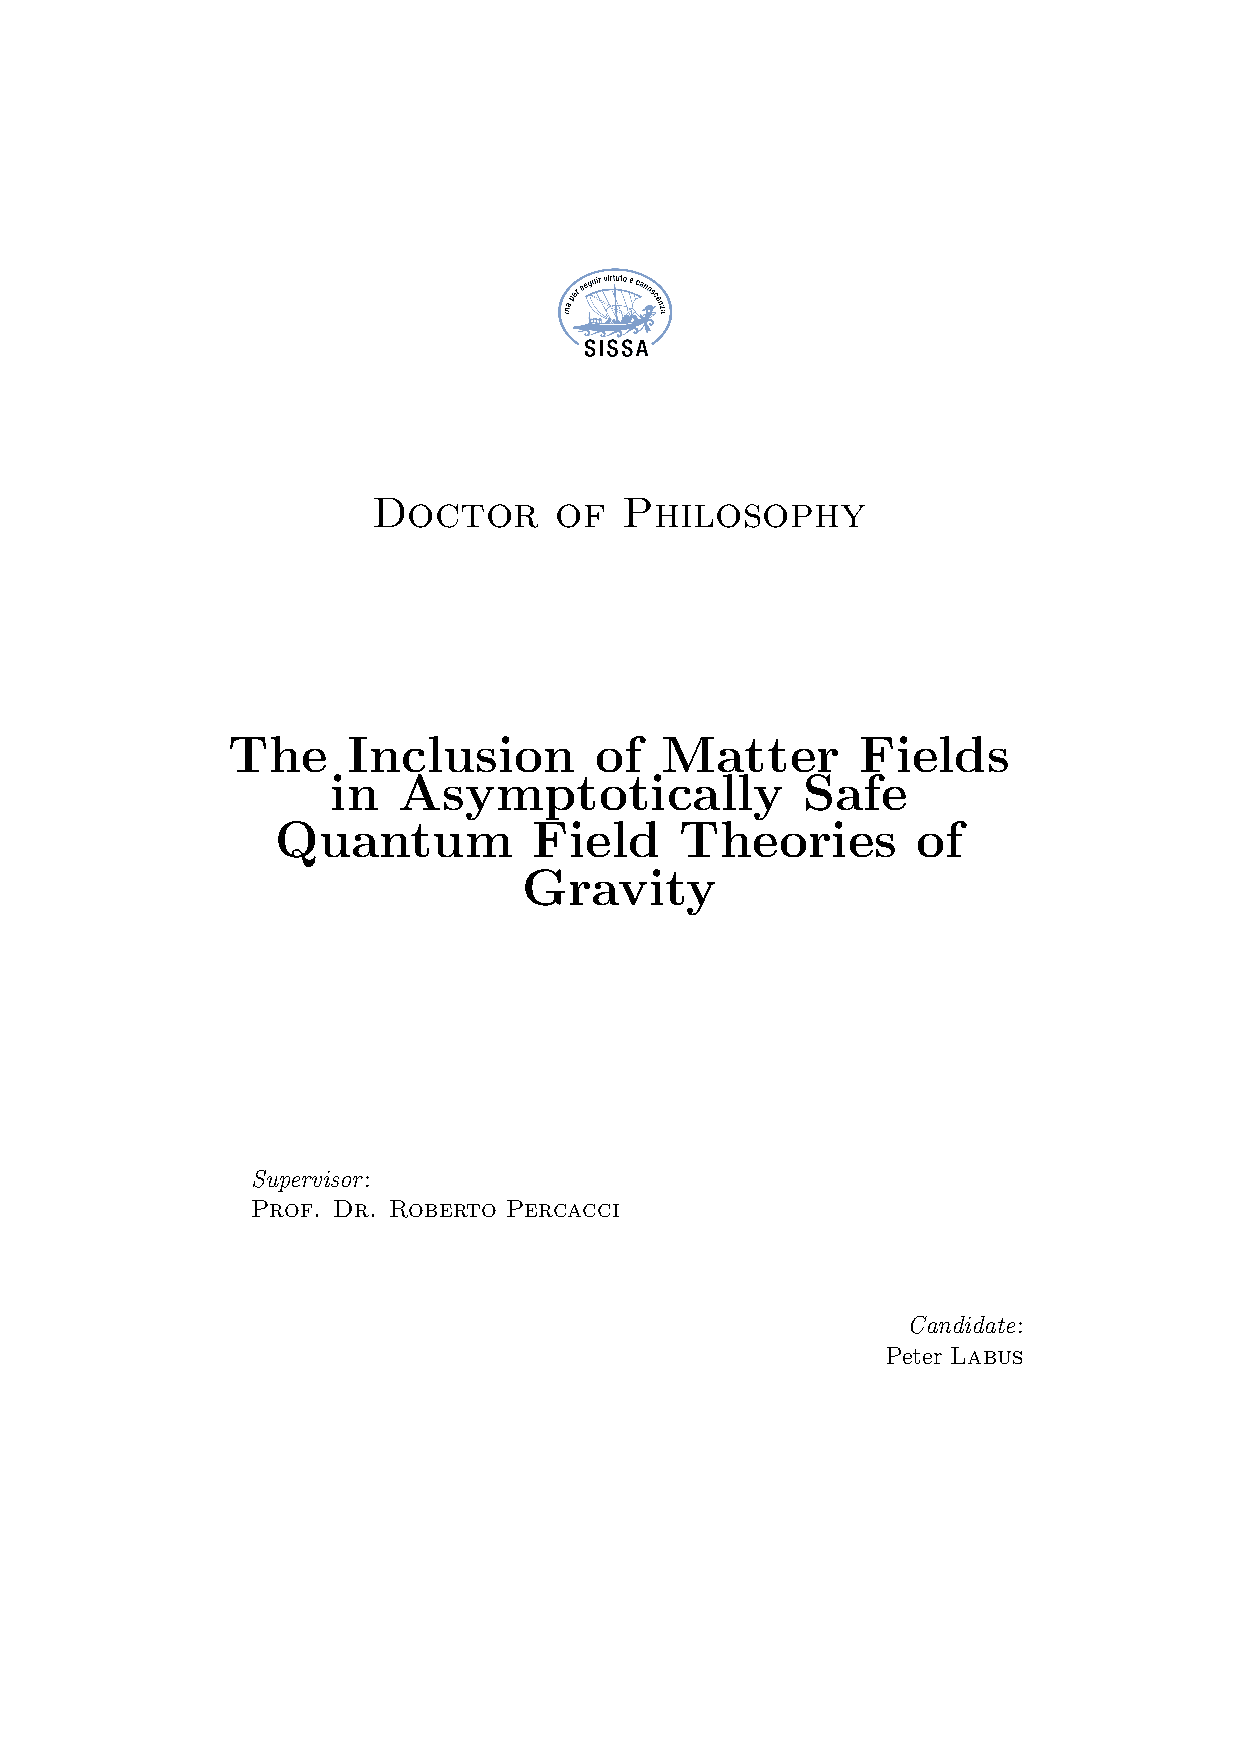
\includepdf{front_page.pdf}

%----------------------------------------------------------------------------------------
% COPYRIGHT PAGE
%----------------------------------------------------------------------------------------

\newpage
~\vfill
\thispagestyle{empty}

\noindent \textsc{PhD Programme in Astroparticle Physics, SISSA Trieste, Italy.}\\

\noindent The research for this PhD thesis project was carried out
under the supervision of Prof.~Dr.~Roberto Percacci with financial support
of a SISSA PhD Fellowship.\\

\noindent \textit{September 2017} % Printing/edition date

%----------------------------------------------------------------------------------------
% PREFACE
%----------------------------------------------------------------------------------------

\chapter*{Preface}
\addcontentsline{toc}{chapter}{Preface}

Blah, blah.

\begin{flushright}
  \textit{Peter Labus, September 2017.}
\end{flushright}

%----------------------------------------------------------------------------------------
% TABLE OF CONTENTS
%----------------------------------------------------------------------------------------

\pagestyle{empty} % No headers

\tableofcontents % Print the table of contents itself

%\cleardoublepage % Forces the first chapter to start on an odd page so it's on the right

\pagestyle{fancy} % Print headers again

%----------------------------------------------------------------------------------------
% INTRODUCTION
%----------------------------------------------------------------------------------------

\chapter*{Introduction}
\addcontentsline{toc}{chapter}{\textcolor{ocre}{Introduction}}


%----------------------------------------------------------------------------------------
% CHAPTER 1
%----------------------------------------------------------------------------------------

\chapter{Scalar Matter}

\section{Introduction}

In the last years many efforts have been devoted to studying the possibility of defining UV complete QFTs
which may describe gravitational interactions,
possibly in the presence of other matter fields.
Such a program is defined within the paradigm of Asymptotic Safety \cite{Weinberg:1980gg}
and can be seen as a bottom-up approach which seeks a consistent extension
to UV of results of low energy effective field theories.
It is related to the construction of the non perturbative RG flow of the effective action,
which should show a UV interacting fixed point (in theory space)
with a finite number of relevant directions.

In a recent paper \cite{Percacci:2015wwa} two of us discussed
fixed-functional solutions
in a scalar-tensor theory with action containing a potential $V(\phi)$
and a generic non-minimal interaction $-F(\phi)R$.
These functions were subjected to a renormalization group flow
depending on a cutoff $k$.
It was found that in generic dimension $d$ the flow equations for the dimensionless
functions $v(\varphi)=k^{-d}V(\phi)$ and $f(\varphi)=k^{2-d}F(\phi)$
of the dimensionless field $\varphi=k^{1-d/2}\phi$
admit some simple exact solutions where $v=v_0$ is constant and
$f=f_0 + f_2 \, \varphi^2$.
These solutions can have interesting applications to cosmology in $d=4$.
\cite{Henz:2013oxa}.
Unfortunately it seems that one of these solutions,
with $f_0$ and $f_2$ both non-zero, does not survive,
at least in the same form, when one applies the
``renormalization group improvement'',
while another, which remains unchanged by the
``renormalization group improvement'',
has $f_0=0$ but $f_2<0$, making its physical relevance questionable.

In this paper we consider the case when
there are $N$ scalar fields, with an $O(N)$-invariant
action of the general form
\begin{align}
  \label{action}
  \int \mathrm d^dx \, \sqrt{g} \,
  \left[ V(\phi) + \frac{1}{2}\sum_{i=1}^N \left( \nabla\phi^i \right)^2 - F(\phi)R \right] .
\end{align}
where now $V$ and $F$ are functions of the radial degree of freedom
and we use the notation $\phi=\sqrt{\sum_i \phi^i\phi^i}$ and for the dimensionless rescaled field
$\varphi=\sqrt{\sum_i \varphi^i \varphi^i}$.
(In section IV it will prove more convenient to think of
$v$ and $f$ as functions of the variable $\rho=\varphi^2/2$.)
The remaining $N-1$ angular degrees
of freedom will be referred to as the Goldstone bosons.
One of the main results of this note is to show that in the case
when $N>1$ there exists also another solution with $f_0=0$ and $f_2>0$.

The other main result will be the confirmation,
on employing a standard cutoff of ``type-I''
(in the terminology of \cite{Codello:2008vh}),
of the existence  of an upper bound on the number of scalars in order to obtain a FP with positive $f$.
Such bounds have been discussed earlier but only for minimally
coupled fields.
We will see that the existence of the potential and of the non-minimal interactions does
not substantially change the picture.

In the same scheme for $d=3$ we also discuss the existence
of a non-trivial gravitationally dressed fixed point
and give a specific solution for $N=2$.
Finally we will employ an alternative coarse-graining scheme
in order to test the scheme-dependence of the analytical scaling solutions.


\section{Flow equations}

For the construction of the flow equations we follow the same steps
as in \cite{Percacci:2015wwa}, which we briefly recall.
The calculation is based on the background field method,
but instead of the usual linear classical-background-plus-quantum-fluctuation split we
use an exponential parametrization
for the metric of the form
$g_{\mu\nu}=\bar g_{\mu\rho}(e^h)^\rho{}_\nu$.
This has some concrete practical advantages that will be
mentioned later,
but the original theoretical motivation is that it
respects the non-linear nature of the metric.
The fluctuation field is further decomposed into its irreducible
spin-two, spin-one and spin-zero components $h_{\mu\nu}^{TT}$,
$\xi_\mu$, $\sigma$ and $h$.
Then one calculates the second variation of the action with
respect to the fields, which appears as a central ingredient
in the flow equation.
In order to have a diagonal Hessian we define new scalar fields
that involve a mixture of $\sigma$ and $\phi$.
We then choose a very simple ``unimodular physical gauge''
which amounts simply to suppressing the fields $\xi$ and $h$.
We describe briefly these steps in the Appendix.
Finally we introduce a ``type I'' cutoff, which amounts to replacing
all occurrences of $-\bnabla^2$ by $-\bnabla^2+R_k(-\bnabla^2)$
\cite{Codello:2008vh}.
In particular we will use the cutoff profile function
$R_k(z)=\left(k^2-z\right)\theta\left(k^2-z\right)$~\cite{Litim:2001up}.
Note that this cutoff is ``spectrally adjusted'',
in the sense that it depends on some running couplings,
and also depends explicitly on the background scalar field,
in addition to the background metric.
Later we shall consider also other types of cutoff.

In general dimension $d$ and for any number of scalars,
denoting by a dot the derivative with respect to RG time $t=\log k$,
the full flow equations are
\begin{align}
  \dot v &= - d \, v + \frac{1}{2} (d-2) \, \varphi \, v'
    + c_d \; \frac{(d-1) \left( d^2 - d - 3 \right)} {d+2}
    + c_d \; \frac{ (d-2) \, (d+1) \left[ 2 \dot f - (d-2) \varphi f' \right] }{4 \left( d+2 \right) f} \nonumber \\[3mm]
  & + c_d \; \frac{ 2 \left( d^2 - 4 \right) f + (d - 2) \left( 1 + v'' \right) \left[ 2 \dot f - 6 f - (d - 2) \varphi f' \right] }
                  { 2 \, (d+2) \left[ 2 (d-1) \left( f' \right)^2 + (d-2) f \left( 1 + v'' \right) \right] } \nonumber \\[3mm]
  & + c_d \; \frac{ 4 \, (d - 1) f' \left[ 2 \dot f' + (d - 1) f' - (d - 2) \varphi f'' \right] }
                  { 2 \, (d+2) \left[ 2 (d-1) f'{}^2 + (d-2) f \left( 1 + v'' \right) \right] }
    + c_d \; \frac{(N-1)\varphi}{\varphi+v'} \,,
  \label{flowvfull}
\end{align}

\begin{align}
  \dot f &= (2-d) \, f + \frac{1}{2} (d-2) \, \varphi \, f'
    - c_d \; \frac{d^6 - 2 d^5 - 15 d^4 - 46 d^3 + 38 d^2 + 96 d - 24}{12 (d+2) (d-1) d} \nonumber \\[3mm]
  & - c_d \; \frac{ \left( d^5 - 17 d^3 - 60 d^2 + 4 d + 48 \right) \left[ 2 \dot f - (d - 2) \varphi f' \right] }
    { 48 \, (d-1) \, d \, (d+2) \, f } \nonumber \\[3mm]
  & - c_d \; \frac{ (d-2) f f'' + 2 f'{}^2 }
                  { (d+2) f \left[ 2 (d-1) \left(f'\right)^2+(d-2) f \left(v''+1\right) \right]^2 }
                  \times \bigg\{ (d-2) (d+2) f^2 \nonumber \\[3mm]
  &          \quad \quad + (d-1) f'{}^2 \left[ (d-2) \varphi  f' - 2 \dot f \right]
                  + 2 (d - 1) f f' \left[ (2-d) \varphi  f'' + (d+2) f' + 2 \dot f' \right] \bigg\} \nonumber \\[3mm]
  & + c_d \; \frac{1}{ 24 \left[ 2 (d-1) \left(f'\right)^2+(d-2) f \left(v''+1\right) \right] }
                  \times \bigg\{ f' \Big[ (d-2) \varphi  \Big( 4 (d-1) f'' \nonumber \\[3mm]
                  &          \quad \quad + (d-2) \left( v'' + 1 \right) \Big) - 8 (d-1) \dot f' \Big] + 2 (d-2)  \left[ d\, f v''-\dot f \left(v''+1\right) \right] \bigg\} \nonumber \\[3mm]
  & - c_d \; \frac{ d \, (N-1) \varphi }{ 12(\varphi + v' }
    - c_d \; \frac{ (N-1)\varphi f'(\varphi)}{(\varphi + v'{}^2} \,,
  \label{flowffull}
 \end{align}
where we introduced the $d$-dimensional volume coefficient
\begin{align}
  \nonumber
  c_d = \frac{ 1 }{ (4\pi)^{d/2} \; \Gamma(d/2+1) } \,.
\end{align}
The only difference between the case $N=1$ discussed in \cite{Percacci:2015wwa}
and the case of general $N$ is the addition to the beta functionals
of $v$ and $f$ of the contribution of the Goldstone modes,
which can be easily identified by the factor $N-1$.
The ``RG-unimproved'' or ``one-loop''
flow equations can be obtained by replacing in the r.h.s.
\begin{align}
  \nonumber
  \dot f  \mapsto -         (d-2) \, f  + \frac{d-2}{2} \, \varphi \, f' \,,
  \qquad
  \dot f' \mapsto - \frac{d-2}{2} \, f' + \frac{d-2}{2} \, \varphi  \, f'' \,.
\end{align}
which is equivalent to setting $\dot F$ and $\dot F'$
to zero in the equation for the dimensionful functions $V$ and $F$.


%%%%%%%%%%%%%%%%%%%%%%%%%%%
\section{Scaling solutions}
%%%%%%%%%%%%%%%%%%%%%%%%%%%

We list here some simple analytic solutions
that exist in any dimension.
Making the ansatz that $v$ and $f$ are both constant leads
to a fixed point FP1.
Using the simple, unimproved equations, it has the following coordinates:
\begin{align}
  v_* &=   c_d \left[ \frac{ (d-1)(d-2) }{ 2 \, d } + \frac{N-1}{d} \right] \,, \\
  f_* &= - c_d \, \frac{d^5-4d^4-7d^3-50d^2+60d+24}{24 \, d \, (d-1) \, (d-2)}
         - c_d \, \frac{(N-1) \, d}{12 \, (d-2)} \,.
\end{align}
We note that the first fraction in $f_*$ is positive for $d<6.17$.
Thus for $N=1$ this is an upper bound on the dimension
dictated by positivity of Newton's constant.
Having additional scalars lowers this bound.
The bound becomes lower than four between $N=11$ and $N=12$.
Thus, the fixed point has negative Newton's constant
when there are more than $11$ scalars, a result that is in
rough agreement with previous calculations \cite{Dona:2013qba}
that also used a similar cutoff.

If we include the RG improvement the coordinates of FP1 change to:
\begin{align}
  v_* &=  c_d \left[ \frac{(d^2-1)(d-2)}{d \, (d+2)} + \frac{N-1}{d} \right] \,, \\
  f_* &= -c_d \, \frac{d^6-2d^5-15d^4-46d^3+38d^2+96d-24}{12 \, d \, (d-1) \, (d^2-4)}
         -c_d \, \frac{(N-1) \, d}{12 \, (d-2)} \,.
\end{align}
Now, for $N=1$ positivity of Newton's constant requires $d<5.73$,
and the bound becomes lower than four between $N=14$ and $N=15$.
Thus, the fixed point has negative Newton's constant
when there are more than $14$ scalars.

If we make the ansatz that $v$ is constant and $f$ is of the
form $f_0 + f_2 \, \varphi^2$, there is a solution FP2
for the unimproved fixed point equations
\begin{align}
  v_*          &= c_d \left[\frac{(d-1) (d-2)}{2 \, d}+\frac{N-1}{d}\right] \,, \\
  f_*(\varphi) &= c_d \left[ \frac{d^5-4 d^4-7 d^3-50 d^2+84 d+24}{24 \, d \, (d-1) \, (d-2)}
                  - \frac{(N-1)(d^2-d+12)}{12 \, (d-1) \, (d-2)}\right]
                  + \frac{\varphi^2}{2 \, (d-1)}\,.
\end{align}
We observe that while $f_2$ is always positive,
$f_0$ becomes negative when either $d$ or $N$ become
too large. For example for fixed $N=2$ this happens at $d\approx 5.8$
and for fixed $d=4$ this happens for $N\approx 5.6$.
The solution is probably unphysical in these cases.

The same ansatz does not yield a solution for the improved equations.
We suspect that there may be a solution
with very similar properties but different functional form.
The search of such generalization is beyond the scope of this paper.

If we make the ansatz that $v$ is constant and $f$ is proportional
to $\varphi^2$ (i.e. that $f_0=0$), the fixed point equation is quadratic and admits two
real solutions FP3 and FP4.
They are the same for the improved and unimproved flow equations.
The expressions for arbitrary $d$ are quite long, so
we only give here the formulae for $d=3$
\begin{align}
  v_* = \frac{N}{18\pi^2} \,, \qquad
  f_* = - \frac{ 9N - 80 \pm \sqrt{9N^2-264N+5296} }{ 96 \, (N-1) } \, \varphi^2 \,,
\end{align}
and $d=4$
\begin{align}
  v_* = \frac{2+N}{128\pi^2} \,, \qquad
  f_* = - \frac{ 6N - 41 \pm \sqrt{4N^2-100N+1321} }{ 48 \, (N-1) } \, \varphi^2 \,.
\end{align}
where the upper sign corresponds to FP3
and the lower sign corresponds to FP4.
We note that FP3 has a finite $N\to1$ limit,
while in the case of FP4 there is a divergence.
In fact for $N=1$ the fixed point FP3 had already been seen
in \cite{Percacci:2015wwa}, but FP4 does not exist in that case.
Imposing that $f>0$ we find that FP3 is always unphysical
while FP4 is acceptable for $0<N<15.33$ in $d=3$
and $1<N<11.25$ in $d=4$.


%%%%%%%%%%%%%%%%%%%%%%%
\section{Large-$N$ limit}
%%%%%%%%%%%%%%%%%%%%%%%

All the solutions described in the previous section
have the property that the function $f_*$ is not
positive if the number of scalars exceeds a certain limit.
In order to confirm that this behaviour persists
we consider here the large-$N$ limit of the flow.
It is very convenient to change variable and use $\rho=\varphi^2/2$
as the argument of the functions $v$ and $f$.
It is easy to see that in the large-$N$ limit both the potentials $v$ and $f$ as well
as $\rho$ scale linearly in $N$.
In particular in such a limit the flow equations,
in terms of all the quantities already rescaled by $N$, read simply
\begin{align}
  \dot v &= - d v    + (d-2) \, \rho \, v' + \frac{c_d}{1+v'} \,, \\
  \dot f &= -(d-2) f + \left[ (d-2) \, \rho - \frac{c_d}{\left(1+v'\right)^2} \right] f'  - \frac{d}{12} \, \frac{c_d} {1+v'} \,.
  \label{eqlargeN}
\end{align}
The fixed point equation for the scalar potential $v$ is the same as in flat space.
There is a solution with a constant potential $v$ and one with a non-trivial one which
is known analytically \cite{Marchais:2012}.
In the first case the solution to Eqs.~(\ref{eqlargeN}) is given by
\begin{align}
  v = \frac{c_d}{d} \,, \quad
  f = -\left( \frac{d}{12 \, (d-2)} \, c_d + 2 \, a\right) +  2 \, a \, \frac{d-2}{c_d} \, \rho \,,
\end{align}
where $a$ is a constant of integration. For such a line of fixed points it is clear that,
for $d>2$  and for any value of $a$, the function $f$ is unphysical since either the constant
part or the coefficient of $\rho$ are negative.

In order to deal with the  second case with the non-trivial solution for $v$, its equation is best written,
for $d$ not an even integer, in terms of $w(\rho)=v'(\rho)$ in the implicit form
\begin{align}
  \rho = \frac{d \, c_d}{4} \; _2F_1 \left( 2,\, 1 - \frac{d}{2};\, 2 - \frac{d}{2};\, -w \right) .
\end{align}
Therefore the scalar sector presents the Wilson Fisher type global scaling solution for $2<d<4$.
Also the fixed point equation for $f$ can be further simplified in terms of $w$
and defining a new function $g(w)=f(\rho)$ one has
\begin{align}
  0 = -(d-2) \, g + 2 \, w \, g' - \frac{d}{12} \, \frac{c_d}{1+w} \,,
\end{align}
which can be solved analytically and gives the implicit solution
\begin{align}
  f(\rho) = g(w) = - \frac{d \, c_d}{12 \, (d-2)} \; _2F_1\left( 1,\, 1 - \frac{d}{2};\, 2 - \frac{d}{2};\, -w \right) ,
\end{align}
which is always negative for $d>2$ and therefore such a fixed point for $2<d<4$ appears
in the large $N$ limit to lead to negative gravitational interactions in the current formulation.
We also note that in the asymptotic region $\rho\to\infty$ one has $f(\rho)= -\frac{2 }{3 d (d-2) } \rho$.


%%%%%%%%%%%%%%%%%%%%%%%
\section{Stability analysis}
%%%%%%%%%%%%%%%%%%%%%%%

We discuss here the linearisation of the flow in $d=4$ around the fixed point FP1.
We begin with the simpler ``RG-unimproved'' case,
which yields the following linearised equations:
\begin{align}
  0 &= - (\lambda +4) \, \delta v
       + \left[ \varphi - \frac{N-1}{32 \pi^2 \varphi} \right] \delta v'
       - \frac{1}{32 \pi^2} \, \delta v'' \,, \\
  0 &= - (\lambda +2) \, \delta\! f
       + \left[ \varphi - \frac{N-1}{32\pi^2\varphi} \right] \delta\! f'
       + \frac{N-1}{96\pi^2\varphi} \, \delta v'
       + \frac{1}{96\pi^2} \, \delta v''
       - \frac{1}{32\pi^2} \, \delta\! f' \,.
\end{align}
In this case the critical exponents are equal to their classical values:
\begin{align}
  \theta_1 &= 4 \,, \qquad w_1^t = (\delta u, \, \delta\! f)_1 = \vphantom{\frac 11}      ( 1,\, 0) \,, \nonumber \\
  \theta_3 &= 2 \,, \qquad w_3^t = (\delta u, \, \delta\! f)_3 = \vphantom{\frac 11}      ( 0,\, 1) \,, \nonumber \\
  \theta_5 &= 0 \,, \qquad w_5^t = (\delta u, \, \delta\! f)_5 =                     \left( 0,\, -\frac{N}{32\pi^2}+\varphi^2 \right) .
\end{align}
The solution FP1 for the full fixed point equations in $d=4$ has coordinates
\begin{align}
  v^* = \frac{N+4}{128 \pi ^2} \,, \quad
  f^* = \frac{169-12 N}{2304 \pi ^2} \,.
\end{align}
Linearising the full flow equations around this solution
we get the eigenvalue equations for the eigenperturbations:
\begin{align}
  0 &= - (\lambda + 4) \, \delta v
       + \frac{72 \, \lambda}{169 - 12 N} \, \delta \!f
       + \left[ \varphi - \frac{N-1}{32 \pi^2 \varphi} \right] \delta v'
       + \frac{72 \, \varphi}{12N - 169} \, \delta\!f' - \frac{1}{32\pi^2} \, \delta v'' \,, \\
  0 &=   \left[ \frac{3 \, \lambda \, (45-4N)}{12N - 169}-2 \right] \delta\!f
       + \left[ \frac{3 \, (4N - 45) \, \varphi}{12N-169}
       - \frac{N-1}{32\pi^2\varphi} \right] \delta\!f'
       - \frac{1}{32\pi^2} \, \delta\!f'' \nonumber \\
       & \hspace{9.65cm}
         + \frac{N-1}{96\pi^2\varphi} \, \delta v'
         + \frac{1}{96\pi^2} \, \delta v'' \,.
\end{align}
We can study the spectrum of the leading eigenvalues analytically.
We find four relevant and one marginal direction for $N<\frac{45}{4}$,
while for $\frac{45}{4}<N<\frac{169}{12}$ there are only two relevant and one marginal directions,
since $\theta_2$ and $\theta_4$ become negative. In particular
\begin{alignat}{2}
  \theta_1 &= 4 \,,                                   && (\delta v, \, \delta\! f)_1 = \vphantom{\frac 11} (1, \, 0) \,, \nonumber \\
  \theta_2 &= 2 + \frac{68}{ 3 (45 - 4N) } \,, \quad  && (\delta v, \, \delta\! f)_2 = \left( \frac{72}{12 N - 101}, \, 1 \right)  , \nonumber\\
  \theta_3 &= 2 \,,                                   && (\delta v, \, \delta\! f)_3 = \left( -\frac{29 N}{544\pi^2} + \varphi^2, \, \frac{N(169 - 12 N)}{3264\pi^2}\right) , \nonumber\\
  \theta_4 &= \frac{68}{ 3 (45 - 4N) } \,,            && (\delta v, \, \delta\! f)_4 = \bigg( -\frac{3N(48N(3 N - 76)+22475)}{16\pi^2(4N - 45)(6N - 59) (12N - 101)} \nonumber \\
                                                    & && \hspace{1.8cm} + \frac{72}{12N - 101} \, \varphi^2, \,  - \frac{N(12N - 169)(12N-125)} {96\pi^2(4N - 45)(12 N - 101)}+\varphi^2\bigg) , \nonumber \\
  \theta_5 &= 0 \,,                                   && (\delta v, \, \delta\! f)_5 = \bigg( \frac{29 N (N+2)}{17408\pi^4} - \frac{29(N+2)}{272\pi ^2} \, \varphi^2 + \varphi^4, \nonumber \\
                                                    & && \hspace{2.4cm} \frac{N (N+2) (12 N - 227)}{224\pi ^4}-\frac{(N+2) (12 N - 169) }{1632\pi^2} \, \varphi^2 \bigg) .
\end{alignat}
We note that the eigenvalues come in groups
within which they are shifted by two.
This behaviour had already been observed and
explained in \cite{Narain:2009fy}.


%%%%%%%%%%%%%%%%%%%%%%%%%%%%%%%%%%%%%%%%%%%%%%%%%%%%%%%%%%%%%%%%
\section{The gravitationally dressed Wilson-Fisher fixed point}
%%%%%%%%%%%%%%%%%%%%%%%%%%%%%%%%%%%%%%%%%%%%%%%%%%%%%%%%%%%%%%%%

In \cite{Percacci:2015wwa} we looked for scaling solutions in $d=3$
with a potential resembling that of the Wilson-Fisher fixed point.
We concentrated on the unimproved equations,
and found a solution for sufficiently small $\varphi$
whose potential is almost indistinguishable from the
Wilson-Fisher potential, and with a function $f$
that starts out positive at $\phi=0$ but has negative
second derivative, such that it crosses zero at
some critical value $\varphi\approx 0.92$.
The analysis of the solution beyond this critical value
proved hard and we were unable to establish its global existence.
Perhaps more important, the Hessian becomes ill-defined at the
critical point, so that the equations themselves become unreliable.
A little later, using more powerful numerical techniques,
a global solution was found for the improved RG equation \cite{Borchardt:2015rxa}.
The fixed point potential for this solution is again
very similar to the Wilson-Fisher potential,
but the function $f$ now has positive second derivative
and is positive everywhere, avoiding the issues mentioned above.
With hindsight this solution can be seen also with the
simpler techniques used in \cite{Percacci:2015wwa}, such as
Taylor expansion and the shooting method.
Near the origin it has the expansion
\begin{align}
v &= 0.009355 - 0.029266 \, \varphi ^2 + 0.003591 \, \varphi ^4 + 1.14530 \, \varphi ^6 + \dots \,, \nonumber \\
f &= 0.068604 + 0.172245 \, \varphi ^2 - 0.132631 \, \varphi ^4 + 0.39032 \, \varphi ^6 + \dots \,. \nonumber
\end{align}
We have looked for generalizations of this solution for $N>1$.
Treating $N$ as a continuous variable, candidate scaling solutions
can be found with the shooting method.
We show, as an example, in Fig.~\ref{WFN1N2} the cases $N=1$ and $N=2$.
A spiralling structure appears close to the fixed point which is characterized by a very sharp relative peak.
\begin{figure}
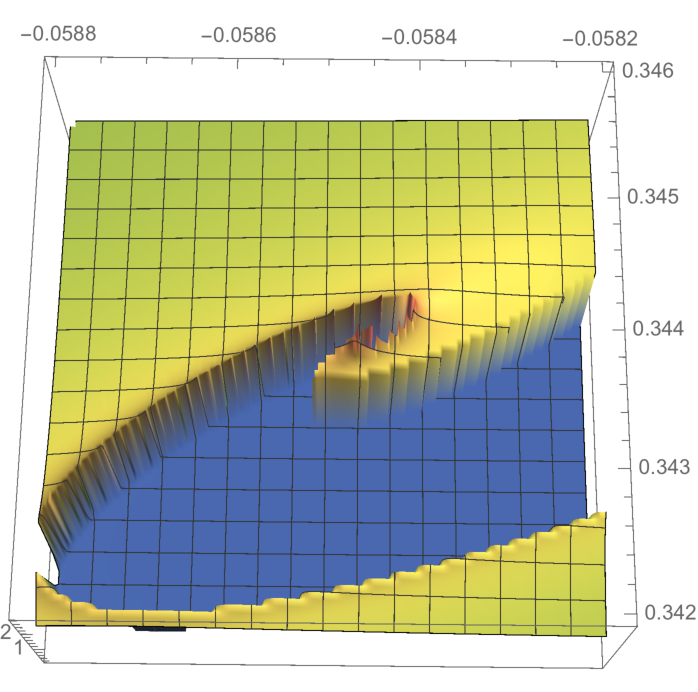
\includegraphics[width=7.5cm]{spike_d3N1.pdf}
\
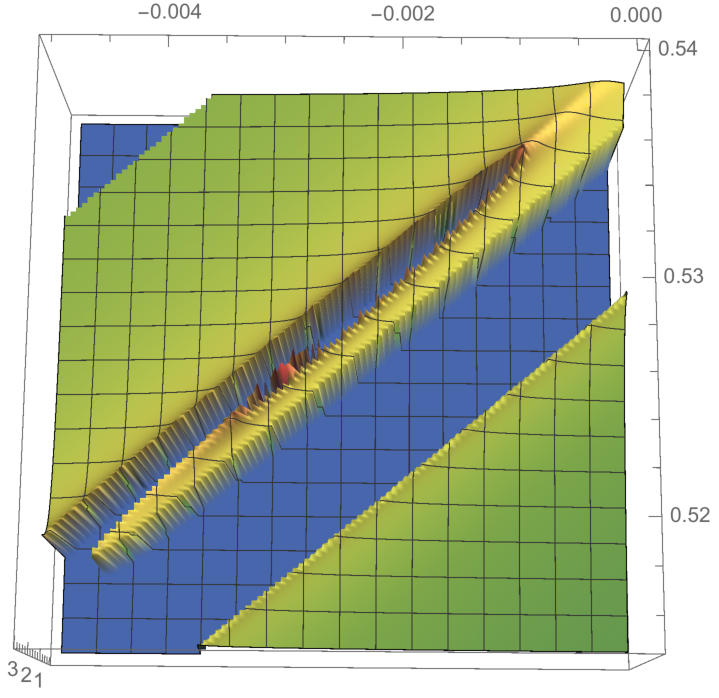
\includegraphics[width=7.5cm]{spike_d3N2.pdf}
\caption{The maximal value of the field reached in the numerical
evolution before encountering a singularity, as a function
of the initial conditions $v''(\varphi=0)$ and $f''(\varphi=0)$,
for the case $d=3$ and $N=1$ (left panel) and $N=2$ (right panel).
A clear spike can be seen in the centre of each figure.
}
\label{WFN1N2}
\end{figure}

For $N=2$ the solution can be approximated near the origin by
\begin{align}
  v &= 0.014669 - 0.001482 \, \varphi ^2 - 0.438516 \, \varphi ^4 + 4.35302 \, \varphi ^6 + \dots \,, \nonumber \\
  f &= 0.053294 + 0.263370 \, \varphi ^2 - 0.570919 \, \varphi ^4 + 1.43572 \, \varphi ^6 + \dots \,. \nonumber
\end{align}
The shape of the potential $v$ shows that the scaling solution is characterised by a broken phase.

The asymptotic behaviour of the solution
for large $\varphi$ is
\begin{align}
  u_{as}(\varphi) &= A \varphi ^6 + \frac{23}{1440 \pi ^4 B \varphi ^2}
                     + \frac{240 \pi ^4 B^2 (16 B+5 N-4)-1357 A}{216000 \pi ^6 A B^2 \varphi ^4} + \dots \,, \\
  f_{as}(\varphi) &= B \varphi ^2 + \frac{23}{36 \pi ^2}+\frac{1219}{25920 \pi ^4 B \varphi ^2}
                     - \frac{71921 A+2160 \pi ^4 B^2 (16 B+5 N-4)}{4665600 \pi ^6 A B^2 \varphi ^4} + \dots \,.
\end{align}
For the case $N=2$ there is a very good match between the numerical solution
found with the shooting method around the origin
and the asymptotic behaviour given above for $A\simeq 5.149$ and $B\simeq 0.273$ around $\varphi\simeq0.65$.
Therefore we consider this as a good candidate for
a global scaling solution for the gravitationally
dressed ${\rm O(2)}$ scalar model.

The critical exponents associated to this fixed point ($N=2$) have not been determined with
sufficient precision using polynomial methods.
We can only report that they are not too far from the values obtained for the $N=1$ case.
More sophisticated numerical methods must be used.


%%%%%%%%%%%%%%%%%%%%%%%%%%%%%%%%%%%%%%%%%
\section{Scalar-free cutoff}
%%%%%%%%%%%%%%%%%%%%%%%%%%%%%%%%%%%%%%%%%

So far we have considered a type-I cutoff which in the gravitational
sector has the general form $F(\bar\phi)R_k(-\bnabla^2)$.
The presence of the prefactor $F$ is useful because the effect
of adding the cutoff results simply in the replacement of
$-\bnabla^2$ by $P_k(\bnabla^2)=-\bnabla^2+R_k(-\bnabla^2)$
in the Hessians.
However, this advantage comes at a price:
the cutoff depends on running couplings
and there is an explicit breaking of the scalar split symmetry
$\bar\phi^a\to\bar\phi^a+\epsilon^a$,
$\delta\phi^a\to\delta\phi^a-\epsilon^a$.
As discussed in \cite{Bridle:2013sra}, already in pure scalar theory
the presence of the scalar background field
in the cutoff action can lead to unphysical results.
This argument casts doubts on the use of these cutoffs,
and it is important to explore also cutoffs that
do not have a prefactor $F$.
In the Einstein-Hilbert truncation, where $F=1/(16\pi G)$,
such cutoffs were called ``pure'' \cite{Narain:2009qa}.
Here we shall call them ``scalar-free''.
It is important to keep in mind that any cutoff still
depends on the background metric, and that this dependence will
have to be dealt with by other means, see e.g. \cite{Dietz:2015owa,Becker:2014qya}.
Here we only get rid of the $\bar\phi$--dependence and have the scalar split Ward
identity automatically fulfilled.
In particular we shall add in the diagonal entries for $h^{TT}_{\,\mu\nu}$
and $\sigma''$ of the Hessian given in Eq.~(\ref{hessfinal})  a cutoff $\gamma\, k^{d-2}(k^2-z)\theta(k^2-z)$,
with the same sign of the Laplacian term, to implement the coarse-graining procedure.
For all the other terms we shall use the more common
$(k^2-z)\theta(k^2-z)$.

We do not report here the form of the flow equations in any dimension,
which contains hypergeometric functions.
For $d=4$ the equations read:
\begin{align}
  \dot v &= - 4v + \varphi v' - \frac{1}{8\pi^2}
            - \frac{ f \left[ f (v''+1) \log\left( \frac{ 3 f'{}^2 }{ f (v''+1) } + 1 \right) - 3 f'{}^2 \right] }
                   { 144 \pi^2 f'{}^4 } \nonumber \\
  &         + \frac{ 3 \gamma \left[ - \gamma^2 + 4\gamma f - 2\gamma(\gamma-2f) \log \left( \frac{f}{\gamma} \right) - 3 f^2\right]}
                   { 16 \pi ^2 (\gamma -f)^3}+\frac{(N-1) \varphi }{32 \pi ^2 \left(v'+\varphi \right)} \,,
\end{align}
\begin{align}
  \dot f &= - 2f + \varphi f' + \frac{19}{384\pi^2}
            + \frac{ f \left[\frac{6f'^2\left(f f''+f'^2\right)}{3f'^2+f\left(v''+1\right)}
            - \left(2 f f''+3 f'^2\right)
              \log\left(\frac{3 f'^2}{f(v''+1)}+1\right)\right]}{288 \pi ^2 f'^4} \nonumber \\
  &         + \frac{ 10 \gamma  (\gamma -2 f) (\gamma -f)-5 \gamma  \left(\gamma ^2-3 \gamma  f+4 f^2\right) \log \left(\frac{f}{\gamma }\right)}
                   { 96 \pi ^2 (\gamma -f)^3} \nonumber \\
  &         + \frac{ \gamma\left[-\gamma +(\gamma-2f)\log\left(\frac{f}{\gamma}\right)+f\right]}
                   {96\pi^2(\gamma-f)^2}
            - \frac{(N-1) \varphi  \left(3 f'+v'(\varphi )+\varphi \right)}{96 \pi ^2 \left(v'+\varphi\right)^2} \,.
\end{align}
Unlike (\ref{flowvfull},\ref{flowffull}),
these are transcendental equations and cannot be solved analytically.
For a comparison we discuss
only the  scaling solution FP1
which is defined by $v(\varphi)=v_0$ and $f(\varphi)=f_0$.
With this ansatz the fixed point conditions reduce to
the following algebraic equations
\begin{align}
  \label{eqpureFP1}
  v_0 &= \frac{1}{128\pi^2(\gamma-f_0)^2}\left[ (N-10)\gamma^2-2(N-13)\gamma f_0+(N-4)f_0^2 - 12 \, \gamma^2 \, \frac{ \gamma - 2f_0 }{ \gamma - f_0} \, \log\left(\frac{f_0}{\gamma}\right) \right] \nonumber \\
  0   &= -2f_0-\frac{4N-55}{384\pi^2} -\frac{f_0(\gamma+9f_0)}{96\pi^2(\gamma-f_0)^2} -\frac{\gamma\left(2\gamma^2-6\gamma f_0+9f_0^2\right) \log\left(\frac{f_0}{\gamma}\right)}{48\pi^2(\gamma-f_0)^3}
\end{align}
These can be solved numerically.
The linearization of the flow equation around FP1 yields the following
equations:
\begin{align}
  0 &= - (\lambda+4) \, \delta v
       - \left[\frac{3\gamma\left(3f_0^2+5\gamma f_0-2\gamma^2\right)}
                    {16\pi^2f_0(f_0-\gamma)^3}
       + \frac{3 \gamma ^2 (\gamma -4f_0)}{8\pi^2(f_0-\gamma)^4}\log\left(\frac{f_0}{\gamma}\right)\right]\delta\! f  \nonumber \\
    &  + \left(\varphi-\frac{N-1}{32\pi^2\varphi}\right)\delta v'
       - \frac{1}{32\pi^2} \, \delta v'' \\
  0 &= - (\lambda +2) \, \delta\! f
       + \left[ \frac{\gamma\left(37 f_0^2-11\gamma f_0+4\gamma^2\right)}
                    {96\pi^2 f_0(f_0-\gamma)^3}
       - \frac{\gamma f_0(2\gamma+3f_0)}{16\pi^2(f_0-\gamma)^4} \log\left(\frac{f_0}{\gamma }\right) \right] \delta\! f  \nonumber \\
    &  + \left(\varphi-\frac{N-1}{32\pi^2\varphi}\right)\delta\! f'
       + \frac{N-1}{96\pi^2\varphi} \, \delta v'
       + \frac{1}{96\pi^2} \, \delta v''
       - \frac{1}{32\pi^2} \, \delta\! f''
\end{align}

For $N=1$ and $\gamma=1$ we have $v_{0*}=0.03314$, $f_{0*}=0.01552$.
The relevant eigenperturbations around this solution
can be found numerically and the corresponding eigenvalues are
$-4$, $-2.272$, $-2$, $-0.272$, $0$.
There are therefore four relevant and one marginal couplings.
For $\gamma=0.006$ we have $v_{0*}=0.00353$, $f_{0*}=0.00670$,
which are very close to the values found with the other cutoff in \cite{Percacci:2015wwa}.
The relevant eigenperturbations around this solution
have eigenvalues $-4$, $-2.542$, $-2$, $-0.542$, $0$,
which are also closer the the other cutoff.

For $N=4$ and $\gamma=1$ the fixed point is at $v_{0*}=0.03635$, $f_{0*}=0.01413$.
The linear perturbation analysis around the fixed point gives the following eigenvalues: $-4$, $-2.299$, $-2$, $-0.299$, $0$.
If instead we choose $\gamma=0.006$, we have $v_{0*}=0.00669$, $f_{0*}=0.00549$,
and the eigenvalues are $-4$, $-2.682$, $-2$, $-0.682$, $0$.

In this scalar-free cutoff scheme it is interesting to investigate the solutions of
Eqs.~\eqref{eqpureFP1} for FP1 in the large $N$ limit.
It is easy to see that in this limit they become
\be
v_0\approx \frac{16N-205}{512\pi^2} \quad , \quad
f_0\approx \gamma\exp{\frac{55-4N}{16}}\ .
\ee
We see that this behaviour is very different from the one obtained previously:
in particular $f_0$ becomes exponentially small but never changes sign.
Thus there is apparently no upper bound in $N$ from the requirement of having a positive $f_0$.
This behavior is induced by the interplay between the $\log$ singularity
in $f_0$ and the linear dependence in $N$ in the equations.
This result is probably not physically correct for the following
reason: in the ERGE one should use the Hessian defined as the second
derivative of the Effective Average Action (EAA) with respect to the quantum field.
Instead in order to close the flow equation,
we are using the second derivative of the
EAA with respect to the background field.
Even though the function $F$ does not appear in the cutoff,
it does appear in the denominator, where the coefficient
of $-\nabla^2$ is $F-\gamma k^{d-2}$.
This term is absent with the type-I cutoff and
it is its presence with the scalar-free cutoff that gives rise
to the logarithmic terms in the flow equation.
In a proper bi-metric calculation the coefficient of
$-\nabla^2$ in the denominator of the ERGE
would be $Z_h-\gamma k^{d-2}$, where $Z_h$ is the graviton
wave function renormalization constant.
The argument of the logarithmic term would then be $Z_h/\gamma$
and the beta function of $f$ would probably be regular for $f=0$.

%%%%%%%%%%%%%%%%%%%%
\section{Discussion}
%%%%%%%%%%%%%%%%%%%%

This paper extends earlier investigations of scalar-tensor
gravity, where we used the exponential parametrization of the metric.
The {\it a priori} motivation of this parametrization is that
it respects the nonlinear structure of the space of riemannian metrics.
It appears a posteriori that it leads to better behaved flows:
there are no infrared singularities \cite{Percacci:2015wwa,Falls:2015qga}
and the equations can be made gauge-independent even off-shell
\cite{Falls:2015qga}.
Quite generally, the use of the exponential parametrization
in conjunction with the physical gauge $\xi_\mu'=\nabla_\mu h=0$
leads to simpler equations.
In the theory considered here, they are sufficiently simple
that analytic scaling solutions can be found.
We have given here the form of such solutions in any dimensions
and for any number of scalar fields.
Relative to our earlier work, the advantage of having more than
one scalar field is that there exists a global solution (FP4)
with $f\geq 0$ everywhere.

One interesting by-product of this analysis is the confirmation
of upper bounds on the number of scalars, for compatibility with
a fixed point with positive $f$.
This result is not confirmed when one uses a scalar-free cutoff
but we have argued that this is probably not physically correct.

As is often the case when taking the large $N$ limit we have been
able to construct the exact analytical solutions
and show that they are unphysical in the type-I cutoff scheme.

We have also investigated in $d=3$ the existence of the gravitationally
dressed Wilson-Fisher scaling solution for various finite N.
In particular we have shown that physically acceptable solution do exist
for small $N$ and given details for the case $N=2$.

We hope that these tools will prove useful also in the search
of global solutions for $f(R)$ truncations,
where several results have been obtained recently
\cite{Benedetti:2012dx,Benedetti:2013jk,Demmel:2012ub,Dietz:2012ic,Dietz:2013sba,Demmel:2015oqa},
but a clear picture is still missing.
Another important direction of investigation is the inclusion of other matter fields,
in particular fermions~\cite{Zanusso:2009bs,Vacca:2010mj,Eichhorn:2011pc,Vacca:2015nta}.
If the picture we have found up to now will be confirmed also in more sophisticated truncations,
the possibility to define a consistent QFT of matter-gravity interactions
will be a guidance in the understanding of several aspects of fundamental/effective physics.
We find already interesting to start to investigate possible implications at
phenomenological level for example in cosmology.



%----------------------------------------------------------------------------------------
% CHAPTER 2
%----------------------------------------------------------------------------------------

\chapter{Scalar Matter 2}

\section{Introduction}
%
\subsection{Renormalization Group scale and bimetric structure of gravity}
%
The perturbative non-renormalizability of General Relativity means that,
if we aim at a quantum field theoretic description of gravity, a non-perturbative route is necessary.
An interacting fixed point of the Renormalization Group (RG) flow provides a notion
of non-perturbative renormalizability, known as the asymptotic safety scenario \cite{Weinberg:1980gg}.
Just as asymptotic freedom in non-Abelian gauge theories allows to define quantum field theories that
are consistent and predictive at all scales,
asymptotic safety could play the same role for quantum gravity, or,
indeed, other gauge theories in $d=4$ dimensions \cite{Litim:2014uca, Litim:2015iea}
or beyond \cite{Gies:2003ic}.
Due to the interacting nature of the fixed point,
one cannot quantize small metric fluctuations around a flat (or, e.g., cosmological) background.
Instead quantum fluctuations of the metric can become arbitrarily large.
This clearly suggests that the notion of a given background,
available in the quantization of other gauge theories,
is not present in gravity. This begs the question:
What does it mean to construct a RG flow for quantum gravity?
How to define coarse-graining, when spacetime itself,
and therefore any measure of momentum-scales, is widely fluctuating?

The solution lies in the use of the background field method \cite{Abbott:1980hw},
where we split the full metric according to
\begin{align}
  g_{\mu\nu}=\bar g_{\mu\rho}(e^h)^\rho{}_\nu.
  \label{exppara}
\end{align}
We then define the path-integral over all metric configurations as the path-integral
over the fluctuation field $h_{\mu \nu}$,
and the background metric $\bar{g}_{\mu \nu}$ can be used to set a scale.
In particular, the fluctuation field can be decomposed into eigenfunctions of the background
covariant Laplacian $-\bar{D}^2$, and those eigenmodes with large eigenvalues are declared to
be the ``high-momentum" modes. In an RG flow from the ultraviolet (UV) to the infrared (IR),
those modes are integrated out first.
It is important to realize that the fluctuation field can have arbitrary amplitude,
so this split does not entail a perturbative treatment,
and in fact varying $h_{\mu \nu}$ allows to reach every possible Riemannian metric
$g_{\mu \nu}$ \cite{Demmel:2015zfa}.
The relation \eqref{exppara}, referred to as the exponential parameterization,
has first been studied in the context of functional RG flows in a unimodular
setting \cite{Eichhorn:2013xr,Eichhorn:2015bna},
and has also been argued to be superior to the linear parameterization in the
context of standard gravity \cite{Nink:2014yya, Percacci:2015wwa, Demmel:2015zfa,
Labus:2015ska, Ohta:2015efa, Gies:2015tca}.

In this framework, the effective action at a scale $k$,
where degrees of freedom of momenta higher than $k$ (as determined by $\bar{g}_{\mu \nu}$)
have been integrated out, depends on the background metric and the fluctuation metric,
i.e., $\Gamma_k = \Gamma_k[\bar{g}_{\mu \nu}, h_{\mu \nu}]$.
This dependence is such that one cannot recombine $\bar{g}_{\mu \nu}$
and $h_{\mu \nu}$ to give the full metric.
This ``split-symmetry" breaking is due to two sources:
The first is the gauge fixing term, which gauge-fixes the fluctuations with respect to the background,
e.g., using a harmonic gauge condition
$F_{\nu}=\bar{D}^{\mu}h_{\mu \nu} -\frac{1}{2} \bar{D}_{\nu}h^{\kappa}_{\kappa}$.
The second is the cutoff term, that is introduced into the path integral to implement
a momentum-shell-wise integration: It acts as a mass-like term for fluctuations of low momenta and
therefore has the structure $h_{\mu \nu} R^{\mu \nu \kappa \lambda} (y) h_{\kappa \lambda}$,
where $y=-\bar{D}^2/k^2$ and $-\bar{D}^2$ denotes the background-covariant
Laplacian\footnote{$R^{\mu \nu \kappa \lambda}$ should not be confused with the
Riemann tensor.}.
As a consequence, couplings of background operators and fluctuation operators do not share the same
beta function. For instance, one can define a Newton coupling from the prefactor of the $\bar{R}$ term
in the effective action, or from the momentum-squared part of the graviton three- point function or
from a graviton-matter vertex.
These three definitions of the Newton coupling obey a different Renormalization Group running.
Modified Ward-identities govern the background-field dependence of the results,
and have to be imposed on the RG flow, but work along these lines is still in its infancy.

In the literature on asymptotically safe gravity, many results are obtained within a
single-metric approximation, where the difference between background couplings and fluctuation couplings
is ignored. There, one finds an interacting fixed point with a finite number of relevant couplings,
i.e., free parameters
\cite{
  Reuter:1996cp, Dou:1997fg, Reuter:2001ag, Lauscher:2001ya, Lauscher:2002sq, Litim:2003vp,
  Fischer:2006fz, Machado:2007ea, Eichhorn:2009ah, Codello:2006in, Codello:2008vh,
  Benedetti:2009rx, Eichhorn:2010tb, Groh:2010ta, Manrique:2011jc, Rechenberger:2012dt, Benedetti:2012dx,
  Dietz:2012ic, Falls:2013bv, Benedetti:2013jk, Ohta:2013uca, Demmel:2014sga, Falls:2014tra, Falls:2015qga,
  Falls:2015cta, Gies:2015tca, Demmel:2015oqa}.
% For reviews, see \cite{ASreviews}.

First explorations of the bimetric structure in asymptotically safe quantum gravity have indicated that the
evidence for asymptotic safety from the single-metric approximation is still present when
resolving this approximation
\cite{
  Manrique:2009uh, Manrique:2010mq, Manrique:2010am, Christiansen:2012rx, Codello:2013fpa,
  Christiansen:2014raa, Becker:2014qya, Christiansen:2015rva}.
One should note that at this stage, only few couplings have been considered in a bimetric setting,
and higher-order truncations could yield different results.
As discussed in \cite{Bridle:2013sra} using the example of a scalar field,
a single-metric approximation can result in spurious fixed points,
and a treatment of the full bimetric structure is crucial.
Within gravity-matter systems, a first step in this direction has been done in
\cite{Dona:2013qba, Dona:2014pla}, where the anomalous dimension of the graviton and matter
fields was evaluated in addition to the beta functions of the gravitational background couplings.
In \cite{Christiansen:2014raa, Christiansen:2015rva},
RG flows formulated in terms of fluctuation field gravitational couplings have been
investigated and lend quantitative support to the results for the pure-gravity
case in the single-metric approximation. The system has been extended to include the effect
of matter fluctuations on pure-gravity-couplings in \cite{Meibohm:2015twa}.
%
\subsection{Quantum spacetime and matter}
%
In this work, we will make a step forward in disentangling the running of fluctuation and
of background couplings, focusing on the matter-gravity sector.
From a phenomenological point of view, the matter-gravity couplings are particularly interesting
for several reasons: First of all, these could become relevant in experimental tests of quantum gravity,
e.g. in astrophysical or cosmological settings,
where high enough energies to test quantum gravity effects might become reachable.
Second, the existence of matter in our universe means that a quantum theory
of spacetime by itself is not viable as a physical theory if it cannot accounted for matter as well.
While one could hope that matter ``emerges" as additional effective excitations of spacetime at low scales,
it seems unlikely that the quantum dynamics of spacetime does indeed provide all observed matter
degrees of freedom with the correct properties, as encoded in the intricate structure of the standard model.
Thus, we will here follow the route towards a joint quantum theory of gravity and matter.
In the context of asymptotic safety, this implies that a viable fixed point must exist not only
for the gravitational interactions, but also for matter-gravity interactions and matter self-interactions.
As the Standard Model by itself is most likely not asymptotically safe, the effect of gravity
is conjectured to  induce a fixed point \cite{Shaposhnikov:2009pv},
see, e.g., for evidence in this direction \cite{Zanusso:2009bs, Vacca:2010mj,
Harst:2011zx, Eichhorn:2011pc, Eichhorn:2012va,Oda:2015sma}.
As a step towards showing that this could indeed be the case,
we investigate the flow of a gravity-scalar-vertex,
and show that it admits an interacting ultraviolet fixed point.
We emphasize that the flow of this coupling is independent from the flow of the usual Newton coupling,
defined with respect to gravitational vertices only.
Our result therefore constitutes nontrivial evidence for the potential viability of asymptotic safety
for a joint description of gravity and matter in our universe.

%
\section{Matter-gravity flows: Setup}
%

In the following we will analyse the Euclidean RG flow of the 1-graviton-2-scalar coupling.
To derive its beta functions we will study the scale-dependence of the effective action $\Gamma_k$ which is governed by the Functional Renormalization Group equation \cite{Wetterich:1992yh, Morris:1993qb},
a.k.a. the Wetterich equation:
\be
\partial_t \Gamma_k = \frac{1}{2} {\rm STr} \left[\left( \Gamma_k^{(2)}+R_k\right)^{-1} \partial_t R_k \right].
\ee
The FRGE is formulated in terms of the dimensionless scale derivative $\partial_t = k\partial_k$,
and $\Gamma_k^{(2)}$ denotes the second functional derivative of the flowing action with respect
to the fields (a matrix in field space).
The supertrace $\rm STr$ includes a summation over the fields with an additional negative
sign for Grassmannian fields, and a summation over the eigenvalues of the Laplacian in the kinetic term,
that translates into a momentum-integral on a flat background.
This equation depends on the full, field-dependent nonperturbative regularized propagator
$\left(\Gamma_k^{(2)}+R_k \right)^{-1}$ which takes into account higher-loop effects while
keeping a rather simple  one loop form.
% For reviews, see \cite{FRGreviews}.

%
\subsection{Truncation}
%
Our truncation consist in the Einstein-Hilbert action for the gravitational sector and
a massless minimally coupled scalar field for the matter sector.
To set it up, we start from an auxiliary action $\hat{\Gamma}$ given in terms of the full
metric $g_{\mu \nu}$, which reads
\be
\hat{\Gamma}= \Gamma_{\rm EH}+ S_{\rm gf} + \Gamma_{\rm kin}.
\ee
Herein
\be
\Gamma_{\rm EH} = -\frac{1}{16 \pi G} \int d^4x \sqrt{g} R\,
\ee
and
\be
\Gamma_{\rm kin} = \frac{1}{2} \int d^4x \sqrt{g} g^{\mu \nu}\sum_{i=1}^{N_S}\partial_{\mu}\phi^i \partial_{\nu}\phi^i.
\ee
We drop a possible volume term in our calculation,
as its fluctuations do not enter the RG flow in our choice of gauge, see below.

In particular, we will employ a York decomposition of the fluctuation field
\be
h_{\mu \nu} = h_{\mu \nu}^{TT} + \bar{D}_{\mu}v_{\nu}+ \bar{D}_{\nu}v_{\mu} + \bar{D}_{\mu}\bar{D}_{\nu}\sigma - \frac{1}{4}\bar{D}^2 \bar{g}_{\mu \nu}\sigma + \frac{1}{4}\bar{g}_{\mu \nu}h,
\ee
with $\bar{D}^{\mu}h_{\mu \nu}^{TT}=0=h^{\mu\, \, TT}_{\mu}$ and $\bar{D}^{\mu}v_{\mu}=0$
and  use the unimodular gauge, defined in \cite{Percacci:2015wwa},
which imposes a constant conformal mode, i.e.
\begin{align}
  h = \rm const \,,
\end{align}
in the exponential parameterization.
Moreover, vector fluctuations are also gauged to zero,
leaving contributions of $h_{\mu \nu}^{TT}$ and $\sigma$ to the running couplings.
For details on the Faddeev-Popov ghost sector for this choice of gauge, see \cite{Percacci:2015wwa}.
We will employ a redefinition of the form
\begin{align}
  \sigma \mapsto \sqrt{(\bar{D}^{2})^2+\frac{4}{3}\bar{D}^{\mu}\bar{R}_{\mu \nu}\bar{D}^{\nu}} \sigma \,,
\end{align}
that cancels part of the Jacobian from the York decomposition \cite{Dou:1997fg}.

To calculate the flow, we define a truncation in the following way:
Starting from the action $\hat{\Gamma}$ we expand in powers of $h_{\mu \nu}$ up to fourth order,
and then redefine $h_{\mu \nu} \rightarrow \sqrt{32 \pi G} h_{\mu\nu}$. In the nonperturbative FRG setting,
the running of the prefactors of the terms at different order in $h_{\mu \nu}$ differs.
We thus introduce several different ``avatars" of the Newton coupling, $G_3$, $G_4$, $g_3$,
$g_4$ and $g_5$, and define our truncation to be
\begin{align}
  \Gamma_{k, \, rhs} &= \sqrt{\frac{G_3}{G}} \, \Gamma_{EH}^{(3,0)} + \frac{G_4}{G} \, \Gamma_{EH}^{(4,0)} \nonumber \\
                     & + \sqrt{\frac{g_3}{G}} \, \Gamma_{\rm kin}^{(1,2)} + \frac{g_4}{ G} \, \Gamma_{\rm kin}^{(2,2)} + \left(\frac{g_5}{ G}\right)^{3/2} \, \Gamma_{\rm kin}^{(3,2)}\nonumber\\
                     & + \vphantom{ \sqrt{\frac{g_3}{G}} }\mbox{ quadratic terms }.
  \label{gammarhs}
\end{align}
Here $\Gamma^{(n,m)}$ stands for the terms of $n$-th order in the fluctuation field $h_{\mu \nu}$
and $m$-th order in the scalar field.
Note that the action that contains the scalar fields is quadratic,
so we only have terms with $m=0,2$.
Our redefinition of all separate prefactors of the different vertices allows us to explicitly distinguish
these avatars of the Newton coupling, instead of approximating them all by $G$.
One should not expect a universal definition of the Newton coupling to exist in the nonperturbative
quantum gravity regime, similarly to what has been found in the perturbative regime in \cite{Anber:2011ut}.
As replicas of Newton's coupling, $G_3$, $G_4$, $g_3$, $g_4$ and $g_5$ all have dimensionality $2-d$.
This justifies the different powers with which they appear
in the various terms in (\ref{gammarhs}).

In detail, the different terms on a flat background are given by:
\bea
 \Gamma_{EH}^{(3,0)} &=&-\frac{1}{3!}
2\sqrt{32\pi G}
 \int d^4x\Bigl(\frac{3}{2} h_{\mu\nu}(\partial_{\mu}h_{\kappa\lambda})\partial_{\nu}h_{\kappa\lambda}\nonumber\\
&{}& - 3 h_{\kappa \lambda}(\partial_{\lambda}h_{\mu\nu})\partial_{\mu}h_{\nu\kappa}\Bigr),\label{GammaG3}\\
%
\Gamma_{EH}^{(4,0)}&=& - \frac{1}{4!}
64\pi G
\int d^4x\Bigl( 3h_{\mu\nu}h_{\kappa\lambda} (\partial_{\mu}h_{\kappa\rho})\partial_{\lambda}h_{\rho\nu}\nonumber\\
&+&h_{\nu\kappa}h_{\kappa\rho}(\partial_{\sigma}h_{\mu\nu})\partial_{\mu}h_{\rho\sigma}
-3 h_{\mu\nu}h_{\nu\kappa}(\partial_{\kappa}h_{\rho\sigma})\partial_{\mu}h_{\rho\sigma}\nonumber\\
&+&4 h_{\mu\nu}h_{\nu\kappa}(\partial_{\mu}h_{\rho\sigma})\partial_{\sigma}h_{\rho\kappa}
-2 h_{\mu\nu}h_{\kappa \lambda}(\partial_{\lambda}h_{\nu\rho})\partial_{\rho}h_{\mu\kappa} \nonumber\\
&+& h_{\mu\nu}h_{\kappa\lambda}(\partial_{\rho}h_{\mu\kappa}) \partial_{\rho}h_{\nu\lambda}
\nonumber\\
&-& h_{\mu\nu}h_{\nu\kappa}(\partial_{\rho}h_{\mu\sigma})\partial_{\rho}h_{\kappa\sigma}\Bigr),\label{GammaG4}\\
%
\Gamma_{kin}^{(1,2)} &=& - \frac{\sqrt{32 \pi  G}}{2} \int d^4x \sqrt{\bar{g}} h^{\mu \nu}\sum_{i=1}^{N_S}\partial_{\mu}\phi^i \partial_{\nu}\phi^i,\label{Gammag3}\\
%
\Gamma_{kin}^{(2,2)} &=& \frac{ 32 \pi  G}{2 } \int d^4x \sqrt{\bar{g}} h^{\mu \rho}h_{\rho}^{\phantom{\rho}\nu}\sum_{i=1}^{N_S}\partial_{\mu}\phi^i \partial_{\nu}\phi^i,\label{Gammag4}\\
%
\Gamma_{kin}^{(3,2)} &=& - \frac{(32 \pi  G)^{3/2}}{2}  \int d^4x \sqrt{\bar{g}} h^{\mu \rho}h_{\rho}^{\phantom{\rho}\lambda}h_{\lambda}^{\phantom{\lambda}\nu}\sum_{i=1}^{N_S}\partial_{\mu}\phi^i \partial_{\nu}\phi^i,\nonumber\\
&{}&\label{Gammag5}
\eea
where appropriate symmetrizations are understood implicitly, as $h_{\mu \nu} = h_{\nu \mu}$.
Here, we have already imposed the gauge $h= \rm const$,
and thus the trace of the fluctuation field can be dropped from the vertices.
This simplifies the vertices considerably.

In an abuse of notation, we do not distinguish between dimensionful and dimensionless couplings,
as all our beta functions will always be expressed in terms of the dimensionless couplings, only,
whereas all couplings in Eq.~\eqref{GammaG3}- \eqref{Gammag5} are still dimensionful.

By the subscript $rhs$ in \eqref{gammarhs} we indicate that this action is used to define the
vertices and propagators that enter the Wetterich equation.
In other words, these are the fluctuation-field structures that \emph{induce} the Renormalization Group flow.
In this paper we will not calculate the running of all these couplings but only the beta function
of $g_3$, and the wave-function renormalizations $Z_\Psi$, with $\Psi=({\rm TT},\sigma,S)$.
The wave-function renormalizations $Z_\Psi$ nevertheless couple into the beta-functions of the
essential couplings in a nontrivial way via the anomalous dimensions
\bea
\eta_\Psi &=&-\partial_t\ln Z_\Psi\ .
\eea

The running of $G_3$ has been calculated recently in \cite{Meibohm:2015twa} using a linear
parametrization of the metric and a more conventional gauge.
We find that the simpler structure of the gravity-matter vertex avoids some of the issues that
are encountered with multi-graviton vertices,
and in any case it is of interest to compare the results of different procedures.

The coupled nature of the Wetterich equation clearly prevents us from defining a closed truncation,
in which we can extract the flow of all couplings that we have included on the right-hand side;
thus approximations are necessary in which some couplings contribute to the running of others,
but their running is not calculated.
The remaining couplings in (\ref{gammarhs}) can accordingly be treated in various ways.
Since they enter in the flow equation for $g_3$,
it is better to avoid a truncation where they are set to zero.
Instead, they can be set equal to $g_3$, or treated as free parameters.
We will discuss different possible approximations with respect to these higher-order couplings below.
It is important to realize that if we were to restrict our truncation to $g_3$,
and set all other couplings to zero, all but Fig.~\ref{threevertexdiagsg3} would vanish.
On the other hand, the original action is diffeomorphism invariant,
and accordingly a 1-graviton-2-scalar-vertex is necessarily accompanied by a 2-graviton-2-scalar vertex etc.
It is therefore expected that an improved truncation takes the existence of these couplings---and
the corresponding diagrams---into account.
To close the system of couplings, we clearly have to choose an approximation,
and we will mostly opt for the choice $g_4=g_3$, $g_5=g_3$ in the following
(which is dictated by dimensionality). To check how useful this approximation is,
we keep track of the couplings separately;
however we will not evaluate the flows of the higher-order couplings.

Note an interesting difference of $\beta_{g_3}$ to the running of the background Newton coupling:
As there is no closed scalar loop contributing to $\beta_{g_3}$,
its only dependence on $N_S$ arises through the anomalous dimension $\eta_{\rm TT}$.

%
\subsection{Projection rules}
%
We use the transverse traceless mode $h_{\mu \nu}^{TT}$
(satisfying $h^{TT\; \mu}_{\;\;\;\;\mu}=0$, $\bar{D}^{\mu}h_{\mu \nu}^{TT}=0$)
to define the matter-gravity coupling $g_3$.
As the running of $g_3$ can unambigously be extracted on a flat background,
we will focus on the choice $\bar{g}_{\mu \nu} = \delta_{\mu \nu}$ in the following.

To extract the running of $g_3$, we employ a projection rule as follows:
\be
\partial_t \sqrt{g_3} = \frac{8}{3} \frac{1}{\sqrt{32 \pi}}\left(p_{1\mu}p_{2\nu} \frac{\delta}{\delta h_{\mu \nu}^{TT}(p_3)} \frac{\delta}{\delta\phi(p_1)} \frac{\delta}{\delta\phi(p_2)} \partial_t \Gamma_k \right)\Big|_{(p^2)^2},\label{projectiong3}
\ee
where we use the symmetric configuration for the three momenta,
such that an angle of $2\pi/3$ lies between them, and their absolute value is $|p_1| = |p_2|=|p_3| =p$.
Note that the functional derivative with respect to the TT mode generates the projector
%
\be
\label{projector}
\mathcal{P}^{\rm TT}_{\mu\nu\kappa\lambda}=
\frac{1}{2}\left(T_{\mu
\kappa}T_{\nu \lambda}
+ T_{\mu\lambda}T_{\nu \kappa} \right)
- \frac{1}{d-1}T_{\mu\nu}T_{\kappa\lambda},
\ee
where $T_{\mu \nu}=\delta_{\mu\nu}-p_{\mu}p_{\nu}/p^2$.
As we are using the transverse traceless component of the graviton for the projection,
there is no mixing with nonminimal couplings that arise from the diffeomorphism-invariant
operator $\phi^2 R$, since the first variation of $R$ does not have a transverse traceless
component  on a flat background.
Furthermore, working with a transverse traceless external graviton mode also excludes an admixture
of non-diffeomorphism invariant operators at the same order of momenta,
which might be generated by the flow and which depend on the momenta of the graviton.

Any given vertex contains a large number of different tensor structures,
and these are not necessarily all featuring the same running coupling.
In particular, transverse traceless structures and scalar structures could be expected to exhibit
prominent differences in their running. As a first step into this direction,
we distinguish the wave-function renormalization for the TT mode and the $\sigma$ mode,
$Z_{\rm TT}$ and $Z_{\sigma}$. On the other hand, we do not distinguish the couplings in the same fashion.

To extract the flow of the wave-function renormalizations, we define projection rules as follows:
\bea
\partial_t Z_S
&=& \left( \frac{\partial}{\partial p^2}\frac{\delta}{\delta \phi(-p)}\frac{\delta}{\delta \phi(p)} \partial_t \Gamma_k\right) ,\\
\partial_t Z_{\rm TT}
&=& \left( \frac{\partial}{\partial p^2} \frac{\mathcal P^{\rm TT}_{\mu \nu\kappa\lambda}(p)}{5} \frac{\delta^2}{\delta h^{TT}_{\mu \nu}(p) \delta h^{TT}_{\kappa \lambda}(-p)} \partial_t \Gamma_k\right),\\
\partial_t Z_{\sigma}
&=&-\frac{8}{3} \left( \frac{\partial}{\partial p^2}\frac{\delta}{\delta \sigma(-p)}\frac{\delta}{\delta \sigma(p)} \partial_t \Gamma_k\right),
\eea
where the right-hand sides are evaluated at $p=0$,
and at vanishing external fields $h_{\mu \nu}^{TT}$, $\sigma$ and $\phi$.


%%%%%%%%%%%%%%%%%%%%%%%%%%%%%%%%%%%%%%%%%%%%%%%%%%%%%%%%%%%%%%%%%%%%
\section{Results for $\eta_{\rm TT}$, $\eta_{\sigma}$ $\eta_S$ and $\beta_{g_3}$}
%%
For our explicit results, we will employ a regulator shape function of the form
$R_{\Psi k}\left(p^2\right) = Z_{\Psi k} (p^2-k^2) \theta(k^2-p^2)$,
with the appropriate wave-function renormalization for all modes,  \cite{Litim:2001up}.

\subsection{Anomalous dimension for the graviton modes}
%

The purely metric diagrams contributing to $\eta_{\rm TT}$,
cf.~Fig.~\ref{etahdiagsgrav} yield the following results.
\bea
\eta_{\rm TT} \big|_{\rm TT-tadpole} &=& \frac{145}{648 \pi}\, G_4\, (6-\eta_{\rm TT} ),\\
\eta_{\rm TT}  \big|_{\sigma- \rm tadpole} &=&  \frac{29}{324 \pi}\, G_4\, (-6+\eta_{\sigma}),\\
\eta_{\rm TT}  \big|_{TT,\,\sigma} &=&  \frac{25}{576 \pi}\, G_3 \, (16-\eta_{\rm TT}-\eta_{\sigma}),\label{TTsigmatwovertexetah}\\
\eta_{\rm TT}  \big|_{\sigma,\,\sigma} &=&  \frac{1}{216 \pi}\, G_3 \, (-31+5\eta_{\sigma}),\label{sigmatwovertexetah}\\
\eta_{\rm TT}  \big|_{TT,\,TT} &=&  \frac{5}{864 \pi}\, G_3 \, (-388+53\eta_{\rm TT} ).\label{TTtwovertexetah}
\eea
 The subscripts in (\ref{TTsigmatwovertexetah}) -- (\ref{TTtwovertexetah})
denote internal TT and $\sigma$ propagators in the two-vertex diagrams, respectively.
Similarly, there are two diagrams containing scalar fluctuations,
one of them a tadpole (cf.~Fig.~\ref{etahdiagsmatter}) which vanishes due to the
momentum-structure of the vertex.
\bea
\eta_{\rm TT}\big|_{\rm S-tadpole}  &=& 0,\\
\eta_{\rm TT}\big|_{\rm S,\,S}  &=& N_S \, \frac{1}{24 \pi} g_3.
\eea

Similarly, our results for the anomalous dimension of the $\sigma$ mode read
\bea
\eta_{\sigma} \big|_{\rm TT-tadpole} &=& \frac{55}{648 \pi}G_4(6-\eta_{\rm TT}),\\
\eta_{\sigma}  \big|_{\sigma- \rm tadpole} &=& \frac{11}{324 \pi}G_4 (-6+\eta_{\sigma}) ,\\
\eta_{\sigma}  \big|_{TT,\,\sigma} &=& \frac{5}{144\pi}G_3 (-16+\eta_{\rm TT}+ \eta_{\sigma}) ,\\
\eta_{\sigma}  \big|_{\sigma,\,\sigma} &=&\frac{1}{432\pi}G_3 (136 - 35 \eta_{\sigma}),\\
\eta_{\sigma}  \big|_{TT,\,TT} &=& \frac{5}{432\pi}G_3(40-23\eta_{\rm TT}) .
\eea

The matter contributions are given by
\bea
\eta_{\sigma}\big|_{\rm S-tadpole}  &=& 0,\\
\eta_{\sigma}\big|_{\rm S,\,S}  &=& N_S  \frac{1}{48 \pi}g_3 (8-3\eta_S).
\eea

In summary, we have
\bea
\eta_{\rm TT}&=&N_S\frac{1}{24 \pi}g_3 + \frac{1}{1728 \pi} G_3 (-2928 + 455 \eta_{\rm TT} - 35 \eta_{\sigma}) \nonumber\\
&{}&- \frac{29}{648 \pi} G_4 (-18+5 \eta_{\rm TT} - 2 \eta_{\sigma}),\label{etaTTcomplete}\\
\eta_{\sigma}&=& N_S \frac{1}{48 \pi}(8-3 \eta_S)g_3 + \frac{1}{108 \pi} G_3 (24 - 25\eta_{\rm TT} - 5 \eta_{\sigma})\nonumber\\
&{}& +\frac{11}{648 \pi} G_4(18-5\eta_{\rm TT}+2\eta_{\sigma})
\label{etasigmacomplete}
\eea

Note that the sign of the matter contribution agrees for $\eta_{\rm TT}$ and $\eta_{\sigma}$
and is the opposite one from that in the linear parametrization and deDonder gauge,
\cite{Dona:2013qba}. Since the exponential parametrization and the linear parametrization
can be understood as underlying two distinct definitions of the configuration space for
asymptotically safe quantum gravity, such a difference could possibly persist in extended truncations,
and point towards a difference in the number of relevant directions in the two settings,
see also \cite{Ohta:2015efa}.

The two-vertex diagrams enter with opposite signs in $\eta_{\rm TT}$ as compared to $\eta_{\sigma}$.
This will imply that the two anomalous dimensions will typically have values of similar magnitude
but opposite sign. Thus, setting $\eta_{\sigma} = \eta_{\rm TT}$ does not seem to be a good approximation,
if indeed this trend persists beyond our truncation.
Moreover, this could suggest that even in calculations without a York decomposition,
it might be necessary to disentangle the tensor structures of the graviton,
and work with projection tensors.
Comparing to the anomalous dimension $\eta_h$ for the graviton (without York decomposition)
in the linear parametrization,
we observe that $\eta_{\rm TT}$ has the opposite,
leading order \emph{negative} contribution from the pure-gravity fluctuations,
cf.~Eq. 24 in \cite{Dona:2013qba}.

%%%%%%%%%%%%%%%%%%%%%%%%%%%%%%%%%%%%%%%%%%%%%%%%%%%%%%%%%%%%%%%%%%%%%%%%%%%%%%
%%%%%%%%%%%%%%%%%%%%% First figure with diagrams %%%%%%%%%%%%%%%%%%%%%%%%%%%%%
%%%%%%%%%%%%%%%%%%%%%%%%%%%%%%%%%%%%%%%%%%%%%%%%%%%%%%%%%%%%%%%%%%%%%%%%%%%%%%
\begin{figure}
\centering
\hspace{11mm} 
\includegraphics[width=0.33\linewidth,clip=true,trim=3cm 24cm 14cm 2cm]{gravG.pdf}
\hspace{9mm} 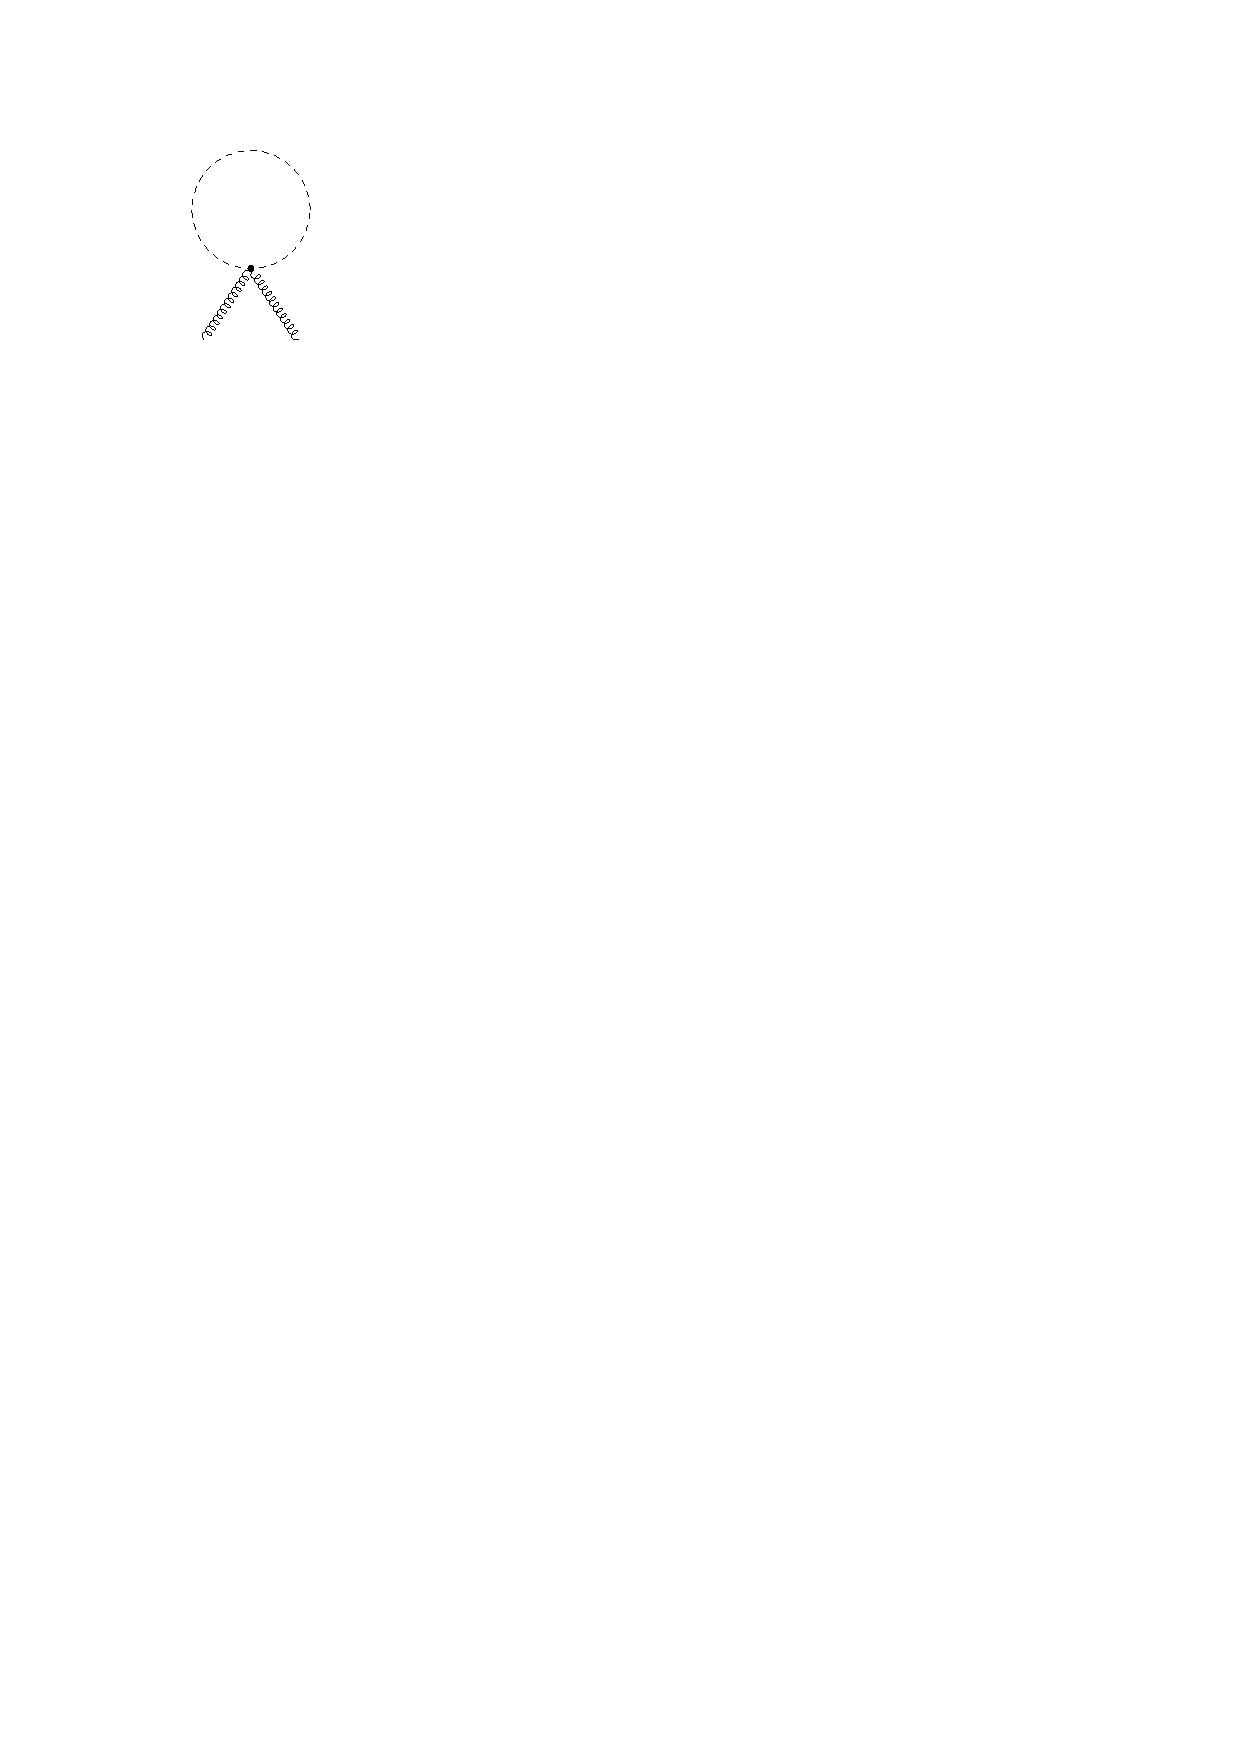
\includegraphics[width=0.33\linewidth,clip=true,trim=3cm 24cm 14cm 2cm]{gravH.pdf}\newline
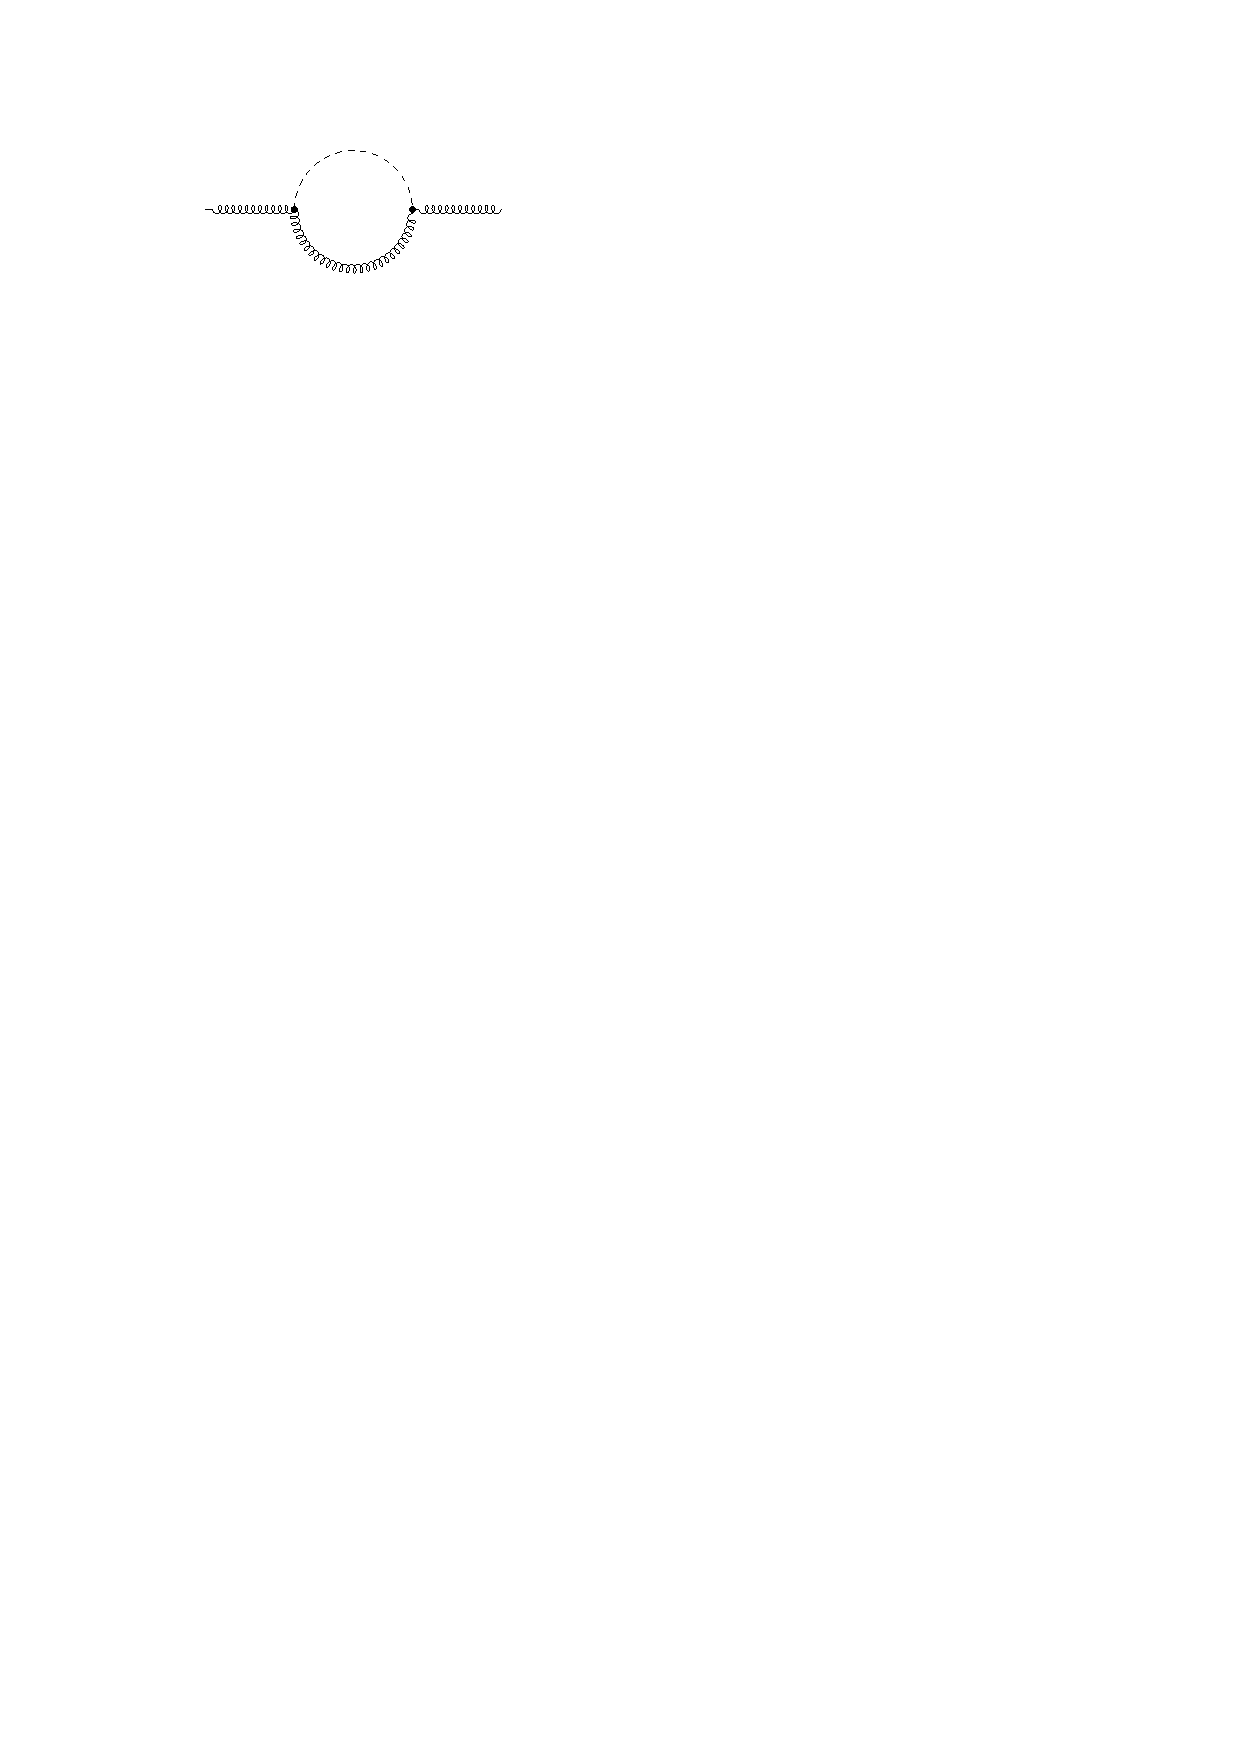
\includegraphics[width=0.45\linewidth,clip=true,trim=3cm 25cm 12cm 2cm]{gravF.pdf}
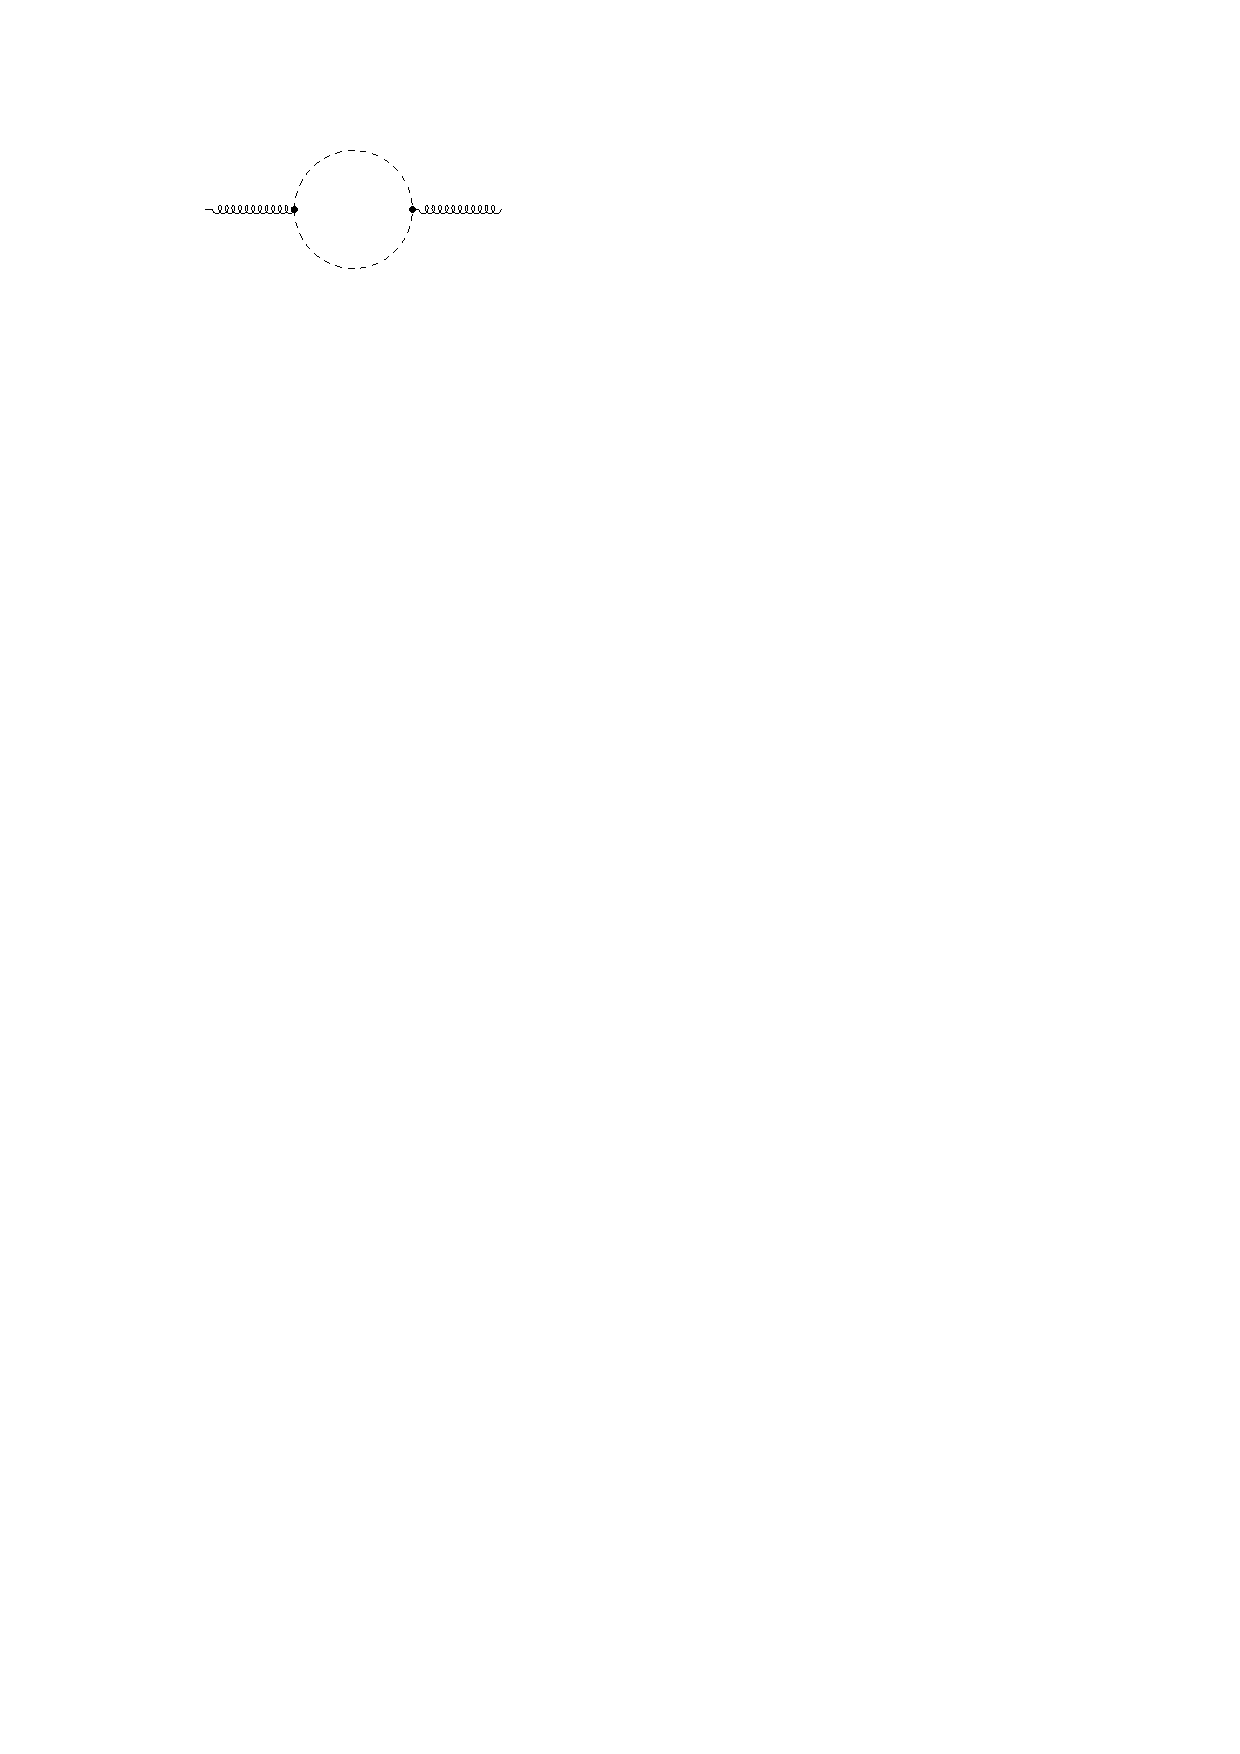
\includegraphics[width=0.45\linewidth,clip=true,trim=3cm 25cm 12cm 2cm]{gravE.pdf}
\hspace{3mm} 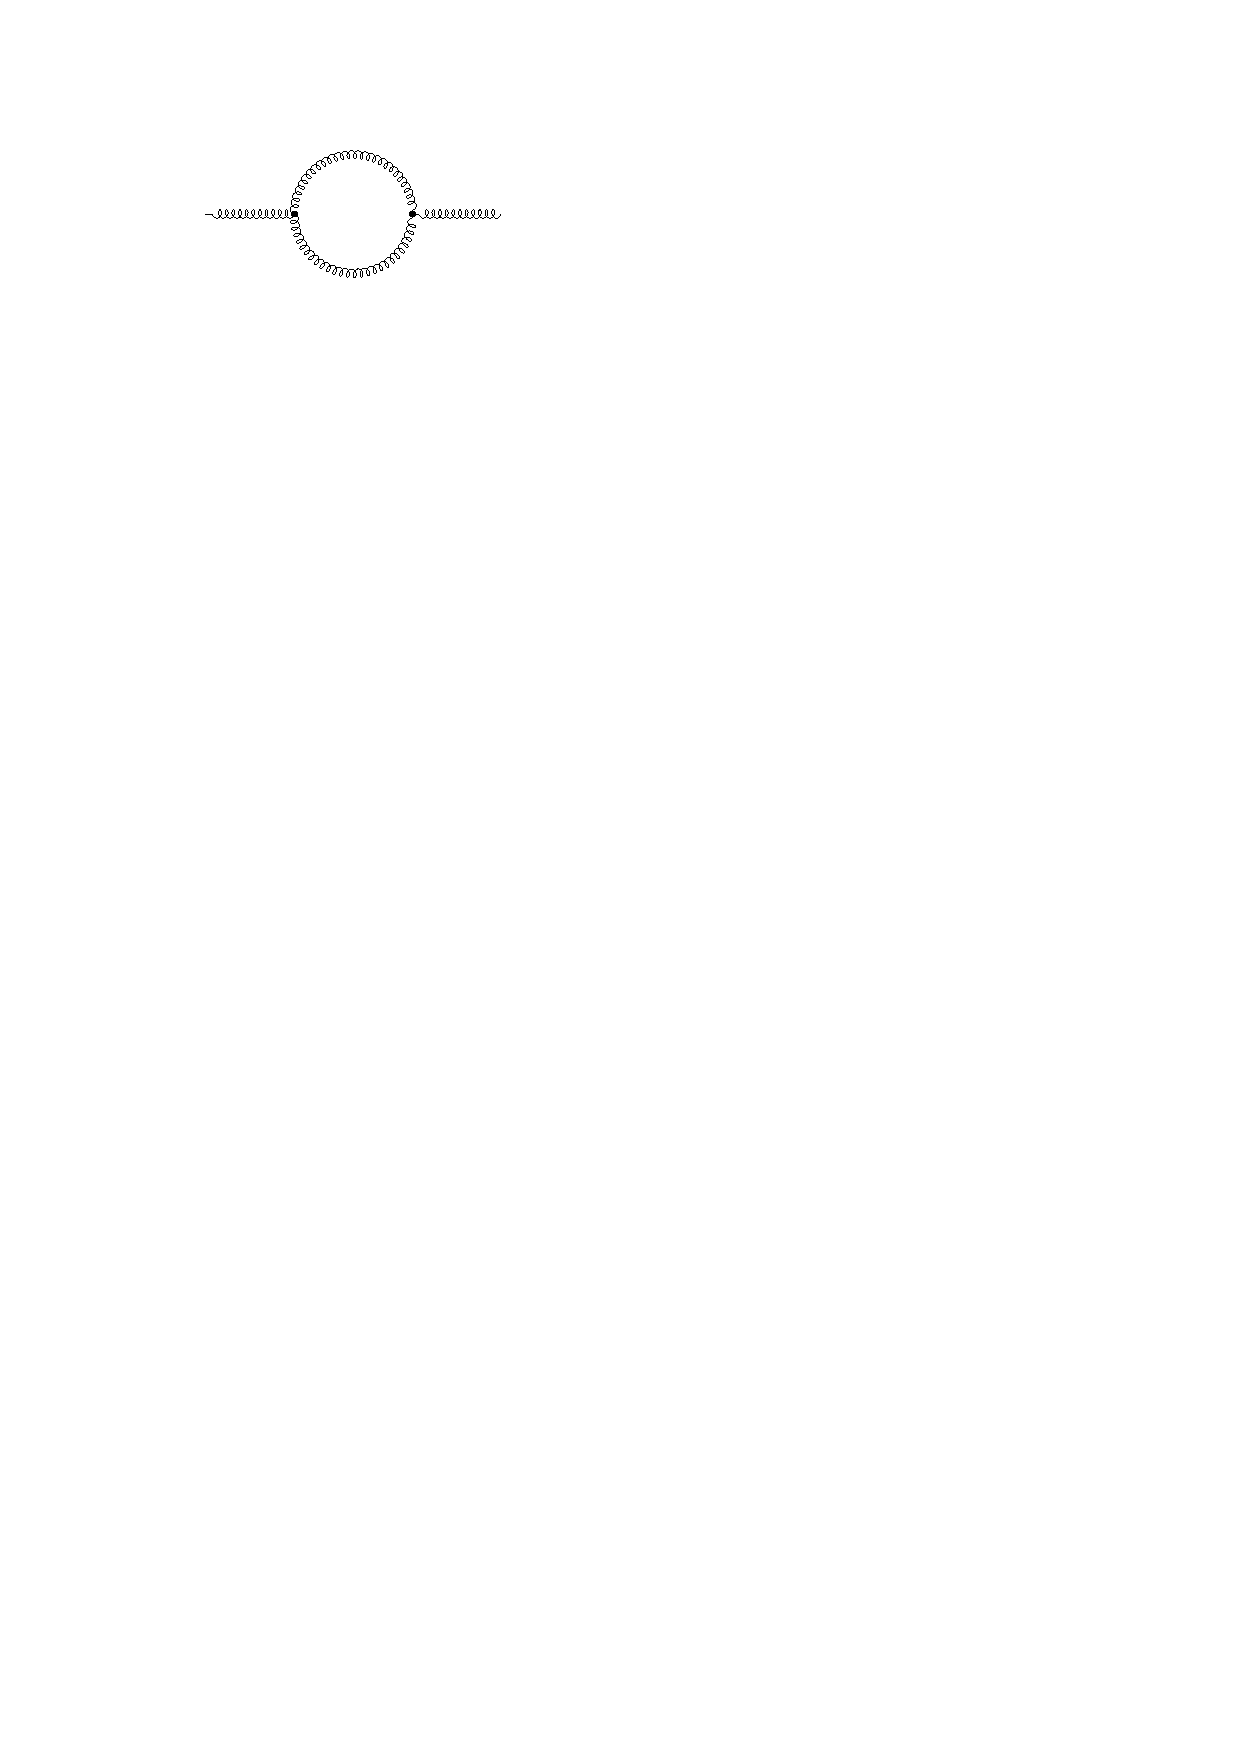
\includegraphics[width=0.45\linewidth,clip=true,trim=3cm 25cm 12cm 2cm]{gravC.pdf}
\caption{\label{etahdiagsgrav} Metric diagrams contributing to the flow of $\eta_{\rm TT}$.
Each diagram with n propagators occurs in n versions with the regulator insertion appearing on each
of the n internal propagators in turn.
Curly lines denote the transverse traceless metric mode and dashed lines the scalar graviton mode.
Similar diagrams with external $\sigma$ lines contribute to the anomalous dimension $\eta_{\sigma}$.}
\end{figure}

%%%%%%%%%%%%%%%%%%%%%%%%%%%%%%%%%%%%%%%%%%%%%%%%%%%%%%%%%%%%%%%%%%%%%%%%%%%%%%
%%%%%%%%%%%%%%%%%%%%% Second figure with diagrams %%%%%%%%%%%%%%%%%%%%%%%%%%%%
%%%%%%%%%%%%%%%%%%%%%%%%%%%%%%%%%%%%%%%%%%%%%%%%%%%%%%%%%%%%%%%%%%%%%%%%%%%%%%
\begin{figure}
\centering

\includegraphics[width=0.33\linewidth,clip=true,trim=3cm 24cm 14cm 2cm]{gravB.pdf}
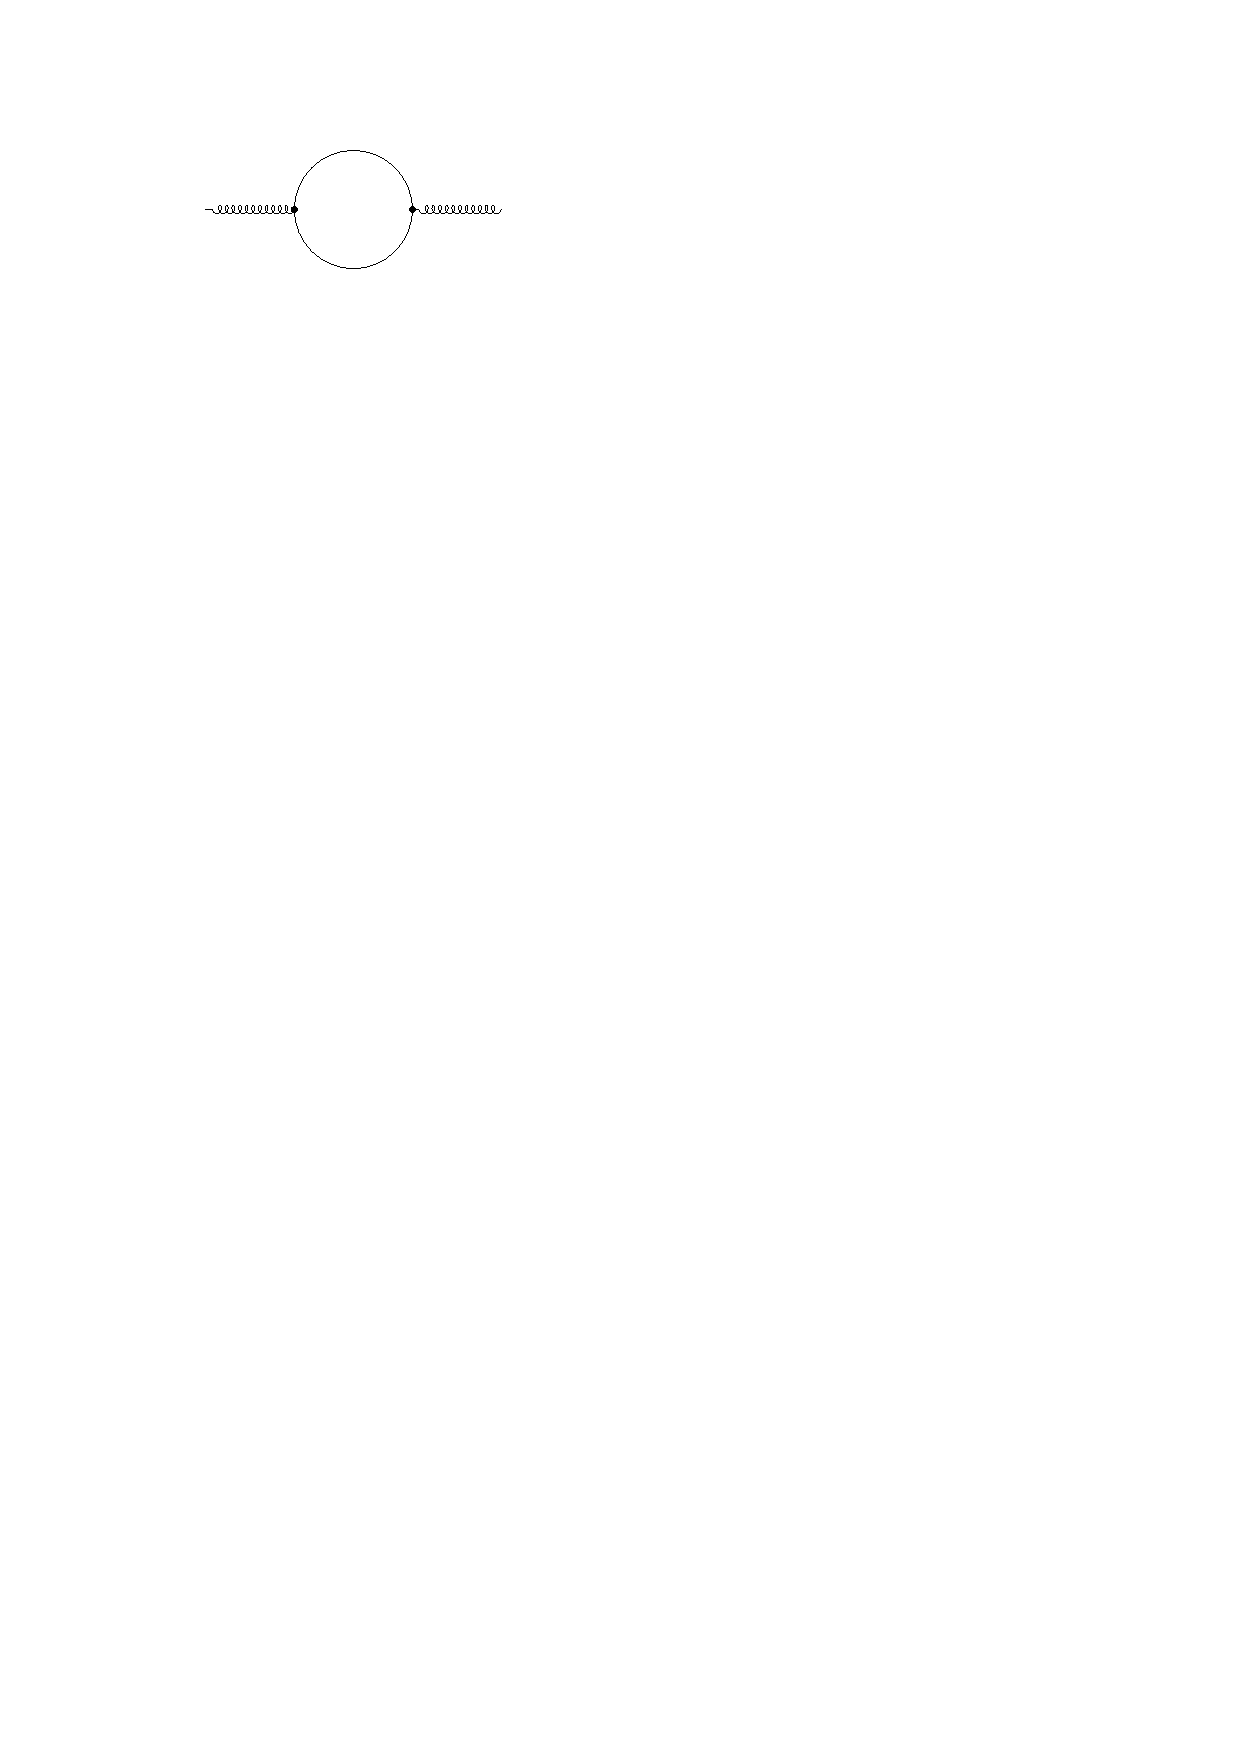
\includegraphics[width=0.45\linewidth,clip=true,trim=3cm 25cm 12cm 2cm]{gravA.pdf}
\caption{\label{etahdiagsmatter} Matter diagrams contributing to the flow of $\eta_{\rm TT}$.
Each diagram with n propagators occurs in n versions with the regulator insertion appearing on each of
the n internal propagators in turn. Curly lines denote the transverse traceless metric mode and continuous
lines the matter scalar.
Similar diagrams with external $\sigma$ lines contribute to the anomalous dimension $\eta_{\sigma}$.}
\end{figure}

%
\subsection{Anomalous dimension for the matter scalars}
%
Similarly, tadpole diagrams and two-vertex diagrams contribute to the flow of $\eta_S$,
cf.~Fig.~\ref{etasdiags}.
\bea
\eta_S\big|_{\rm TT-tadpole} &= &g_4\frac{5}{24\pi}\,(6-\eta_{\rm TT}), \label{etaS1}\\
\eta_S\big|_{\sigma- \rm tadpole} &= & g_4\frac{1}{12 \pi} \, (-6+\eta_{\sigma}),\label{etaS2}\\
\eta_S\big|_{\rm TT-two-vertex} &=& 0, \\
\eta_S\big|_{\sigma-\rm two-vertex} &=& g_3\frac{1}{16\pi} \, (16-\eta_{\sigma}-\eta_S)\label{etaS3}.
\eea

Overall, $\eta_S$ is positive at leading order, when $g_3>0, g_4>0$.
This is the opposite behavior as that observed in the linear parameterization
and the deDonder gauge, \cite{Dona:2013qba}.

%%%%%%%%%%%%%%%%%%%%%%%%%%%%%%%%%%%%%%%%%%%%%%%%%%%%%%%%%%%%%%%%%%%%%%%%%%%%%%
%%%%%%%%%%%%%%%%%%%%% Third figure with diagrams %%%%%%%%%%%%%%%%%%%%%%%%%%%%%
%%%%%%%%%%%%%%%%%%%%%%%%%%%%%%%%%%%%%%%%%%%%%%%%%%%%%%%%%%%%%%%%%%%%%%%%%%%%%%
\begin{figure}
\centering
\hspace{11mm} 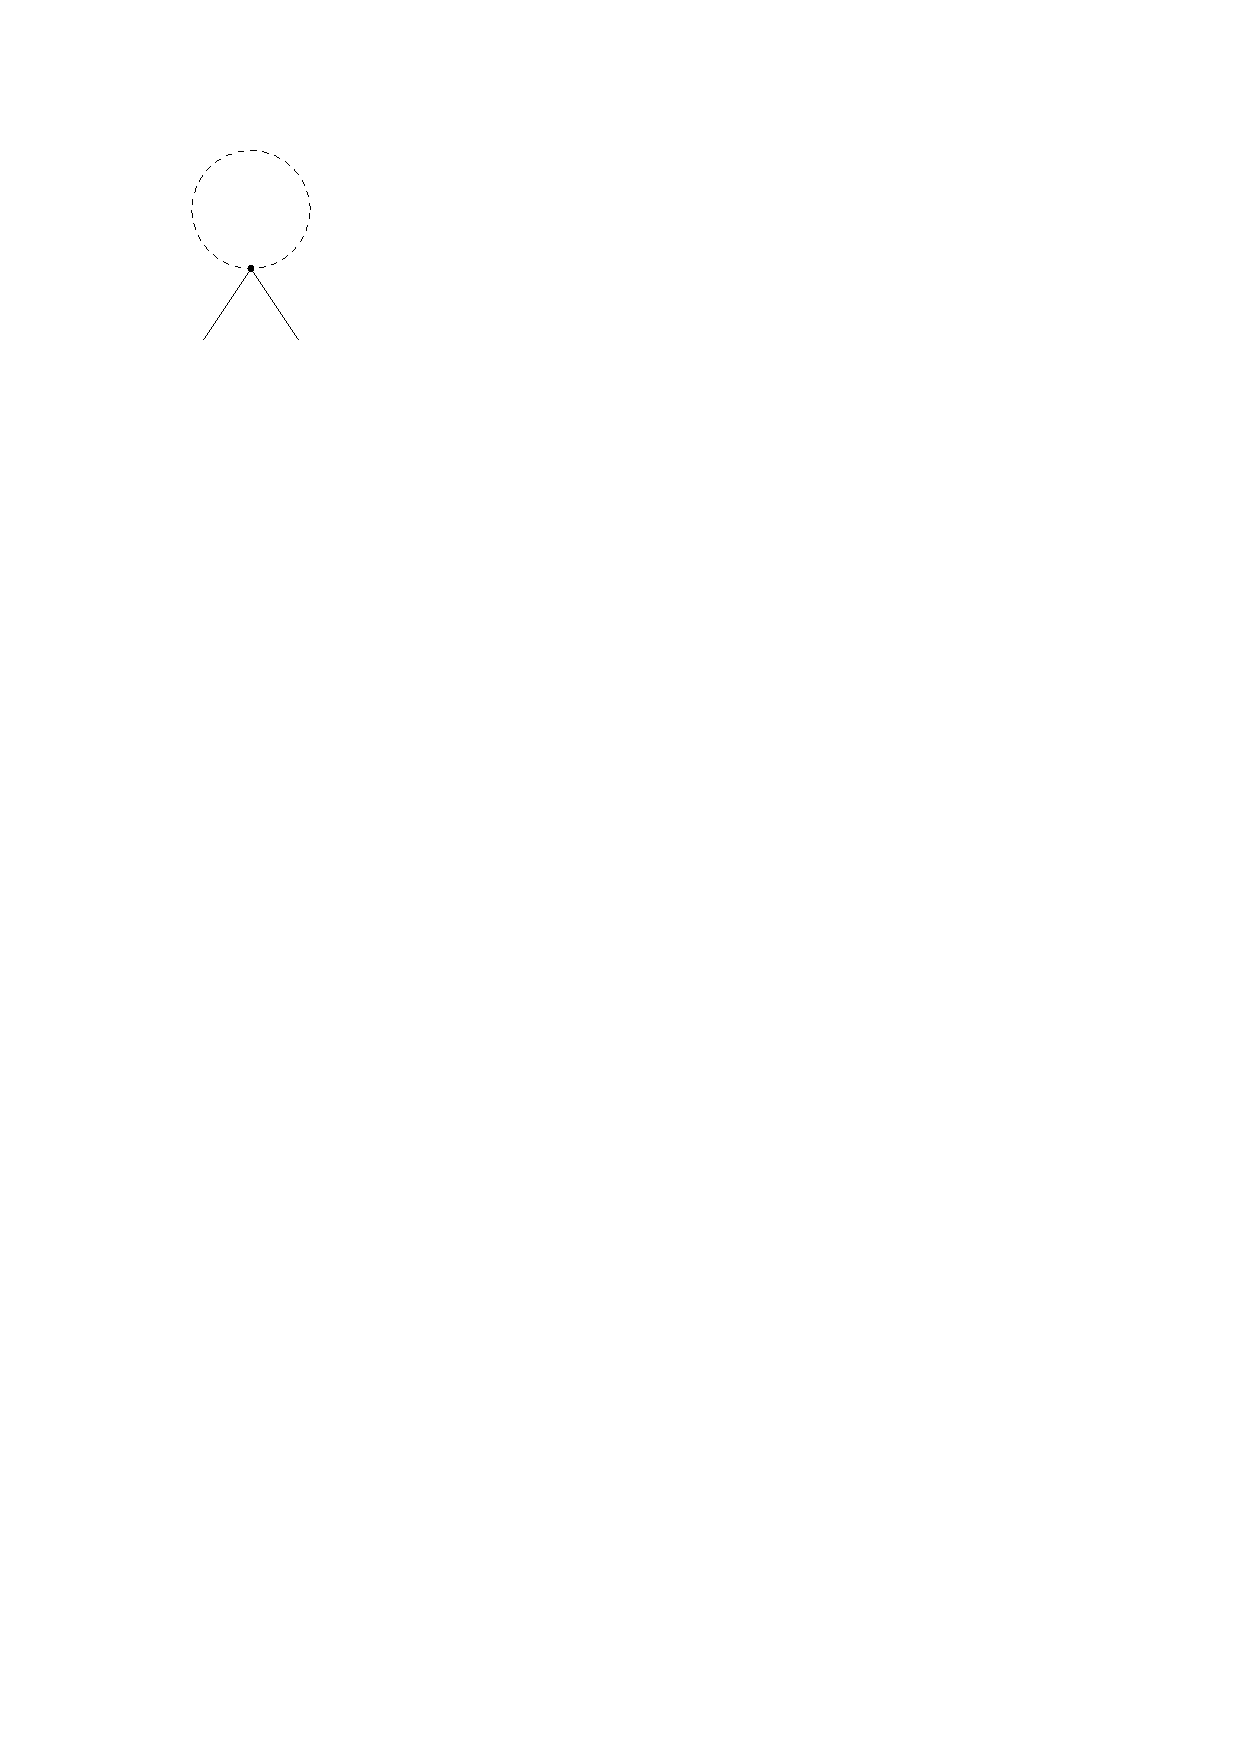
\includegraphics[width=0.33\linewidth,clip=true,trim=3cm 24cm 14cm 2cm]{scalarD.pdf}\quad
\hspace{9mm} 
\includegraphics[width=0.33\linewidth,clip=true,trim=3cm 24cm 14cm 2cm]{scalarC.pdf}\newline
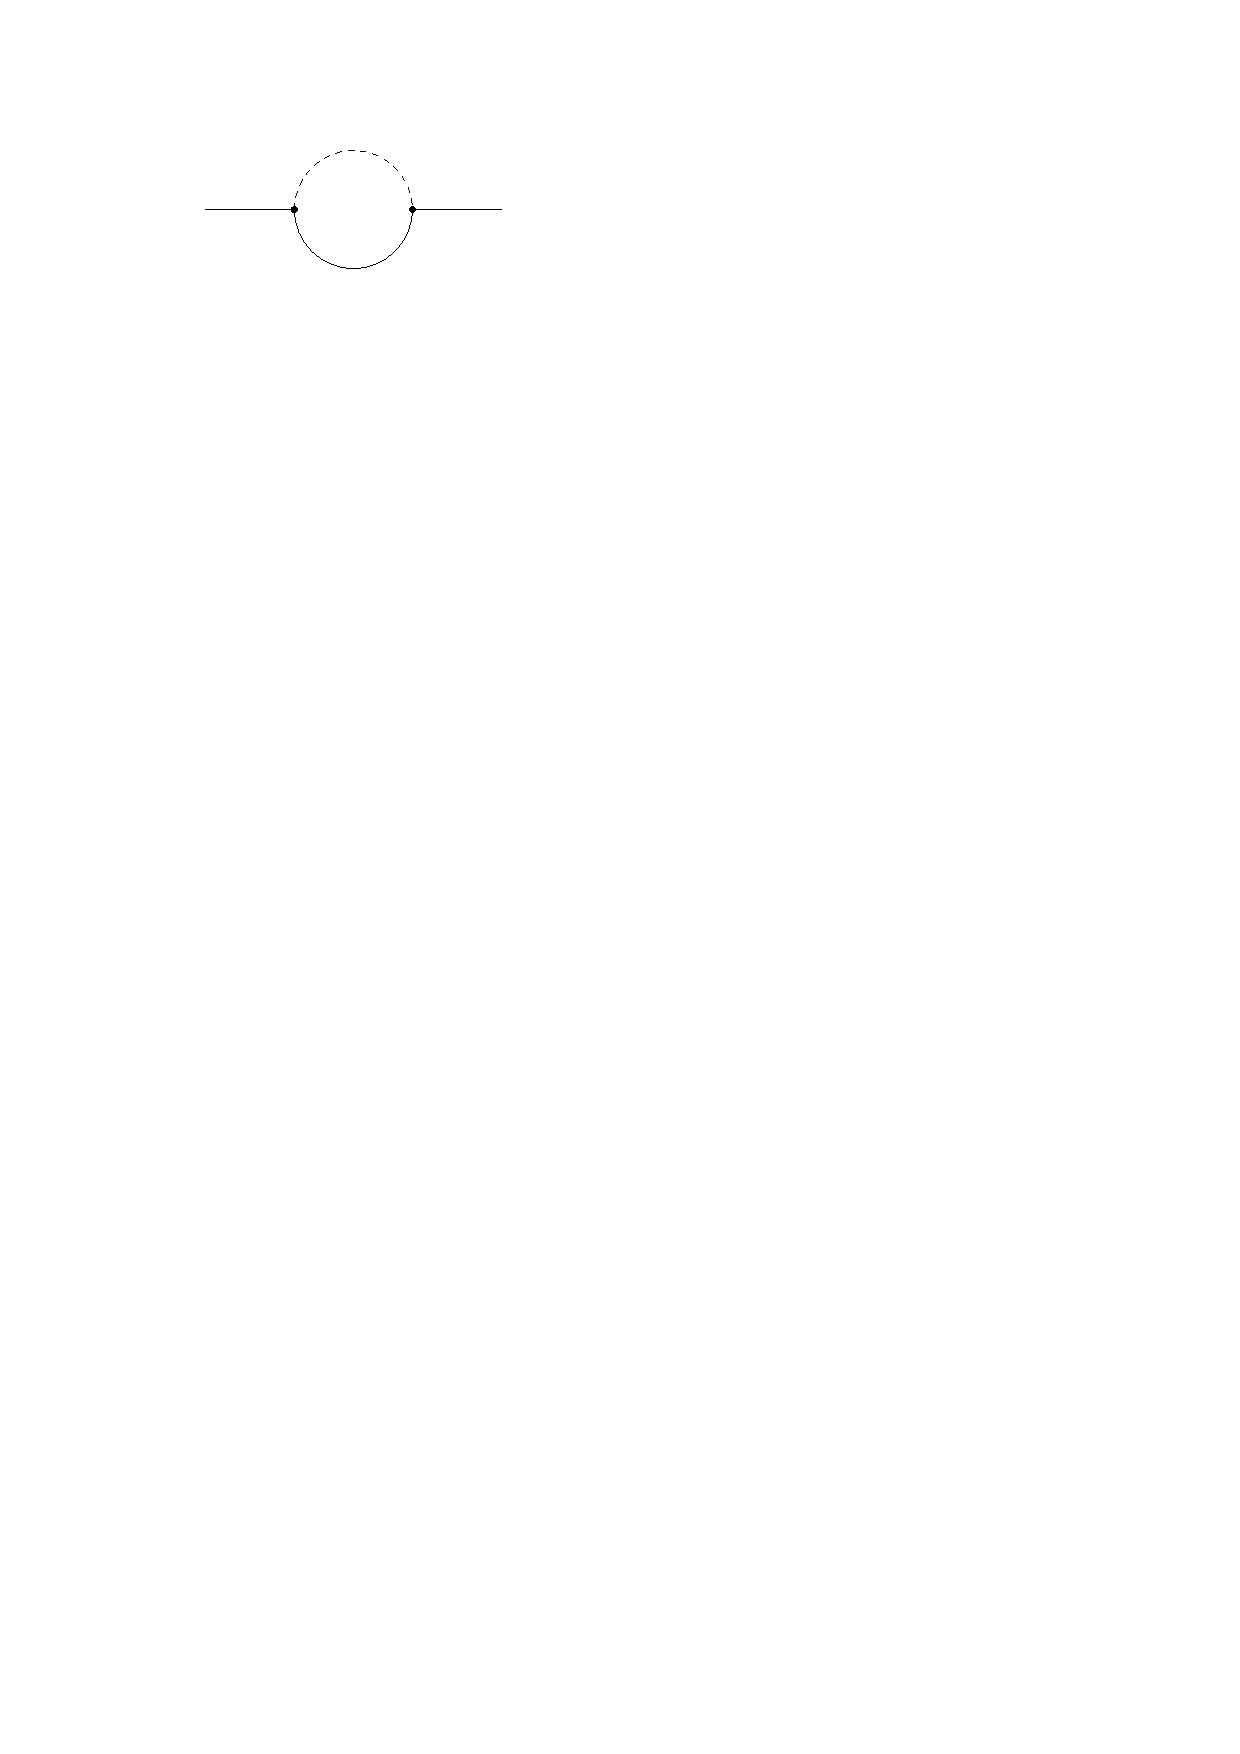
\includegraphics[width=0.45\linewidth,clip=true,trim=3cm 25cm 12cm 2cm]{scalA.pdf}\quad
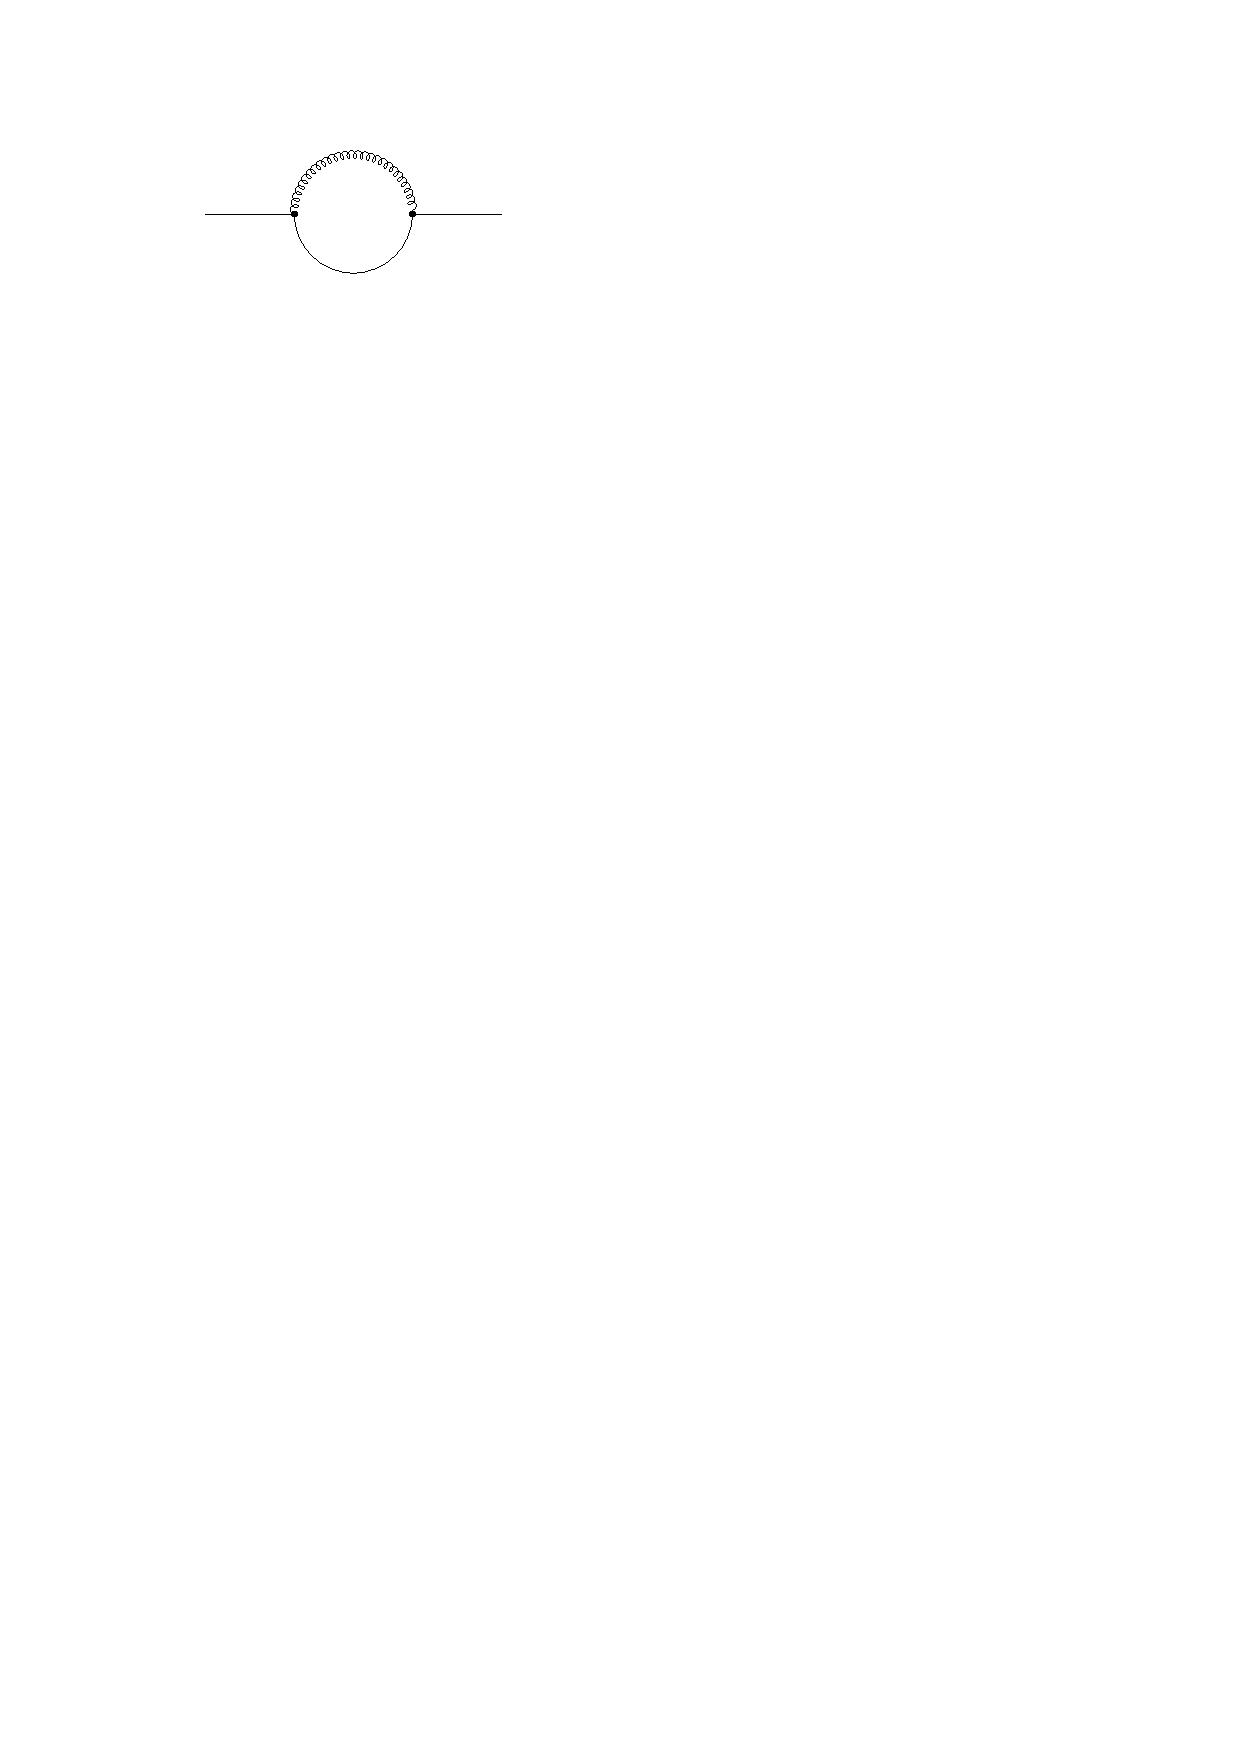
\includegraphics[width=0.45\linewidth,clip=true,trim=3cm 25cm 12cm 2cm]{scalB.pdf}
\caption{\label{etasdiags}Metric diagrams contributing to the flow of $\eta_S$.
Each diagram with n propagators occurs in n versions with the regulator insertion appearing
on each of the n internal propagators in turn.
Curly lines denote the transverse traceless metric mode,
dashed lines the scalar graviton mode and continuous lines the scalar.}
\end{figure}


%
\subsection{Flow of $\sqrt{g_3}$}
%

The flow of the two scalar-one graviton vertex
$\sqrt{g_3}$ is driven by three types of diagrams:
First of all, there are three-vertex diagrams in which all vertices are $\sim \sqrt{g_3}$ themselves,
cf.~Fig.~\ref{threevertexdiagsg3} (note that we do not distinguish between the coupling of two
scalars and one $\sigma$ mode and the coupling of two scalars and the TT mode,
although we use only the latter to read off the running of $g_3$.)
\begin{figure}
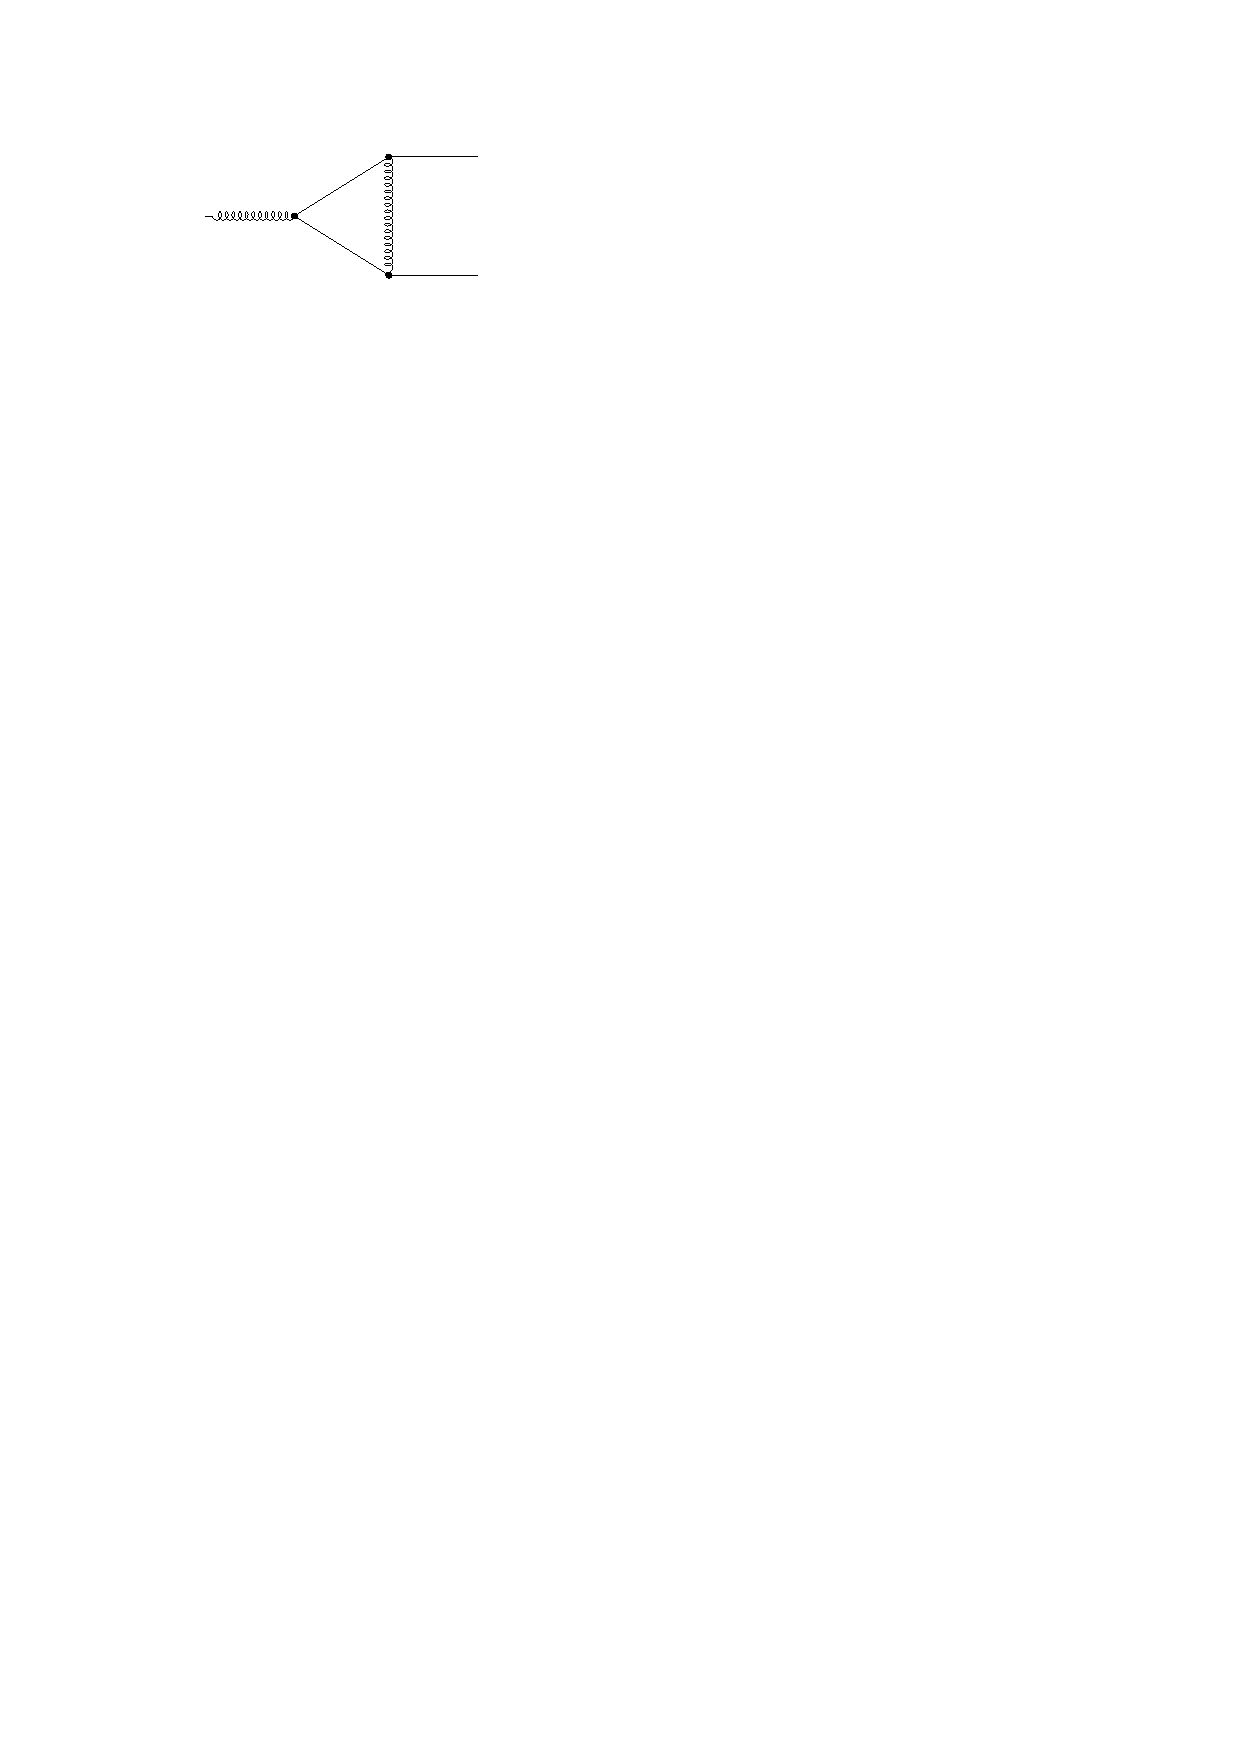
\includegraphics[width=0.45\linewidth,clip=true,trim=3cm 25cm 12cm 2cm]{1a.pdf}\quad 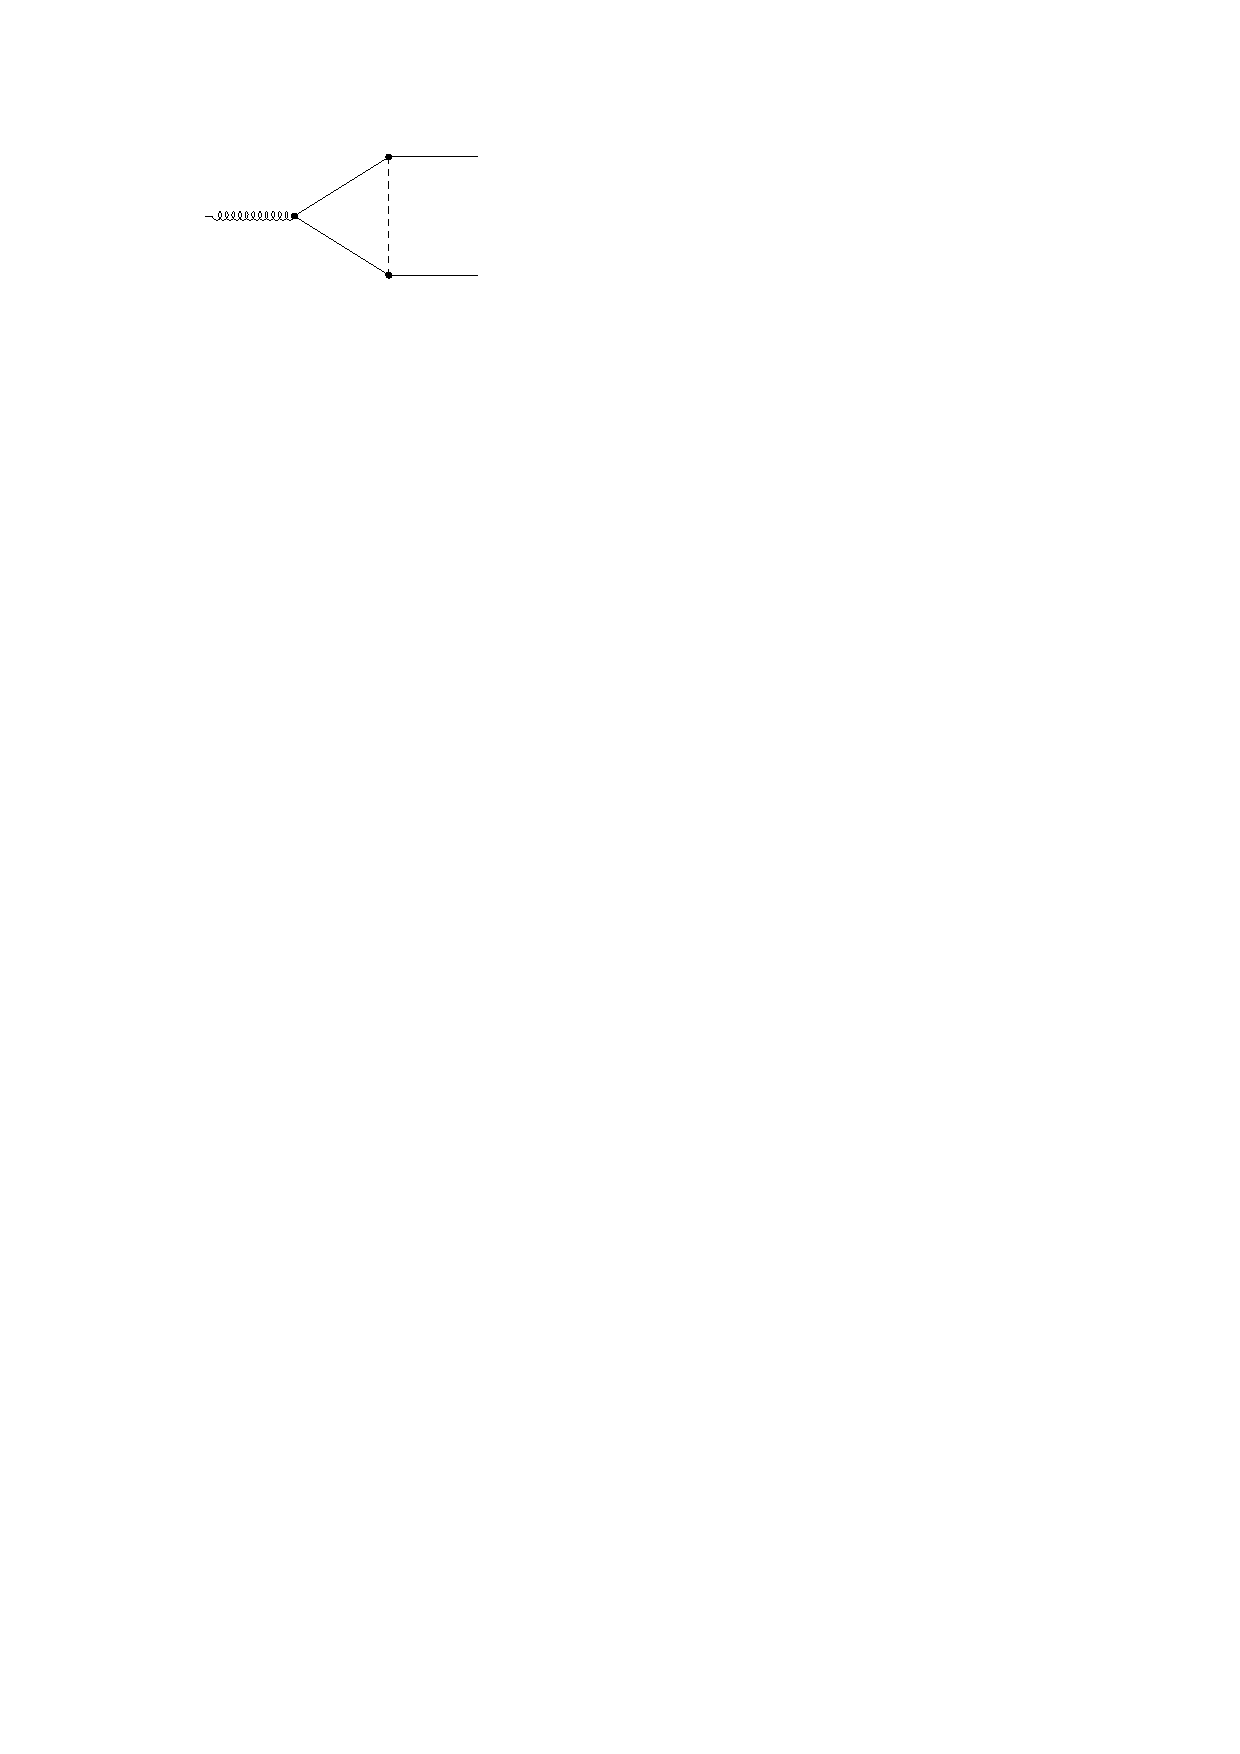
\includegraphics[width=0.45\linewidth,clip=true,trim=3cm 25cm 12cm 2cm]{1b.pdf}\newline
\caption{\label{threevertexdiagsg3} Three-vertex-diagrams contributing to the flow of $\sqrt{g_3}$,
which feature only the coupling $\sqrt{g_3}$ itself at all vertices.
Each diagram with n propagators occurs in n versions with the regulator insertion appearing on each
of the n internal propagators in turn.
Curly lines denote the transverse traceless metric mode,
dashed lines the scalar graviton mode and continuous lines the scalar. }
\end{figure}

These three-vertex diagrams in Fig.~\ref{threevertexdiagsg3} only have a contribution from the $\sigma$ mode;
the transverse traceless mode contributes to the running of the two-scalar-one-graviton-vertex
at a higher order in the momenta, when our projection prescription
\eqref{projectiong3} is used.
Note that the leading-order contribution to $\beta_{\sqrt{g_3}}$ comes with a positive sign.

\bea
\beta_{\sqrt{g_3}}\big|_{\rm TT\, 3-vertex} &=& 0 \\
\beta_{\sqrt{g_3}}\big|_{\sigma \rm\, 3-vertex}  &=&
\frac{1}{80 \pi} g_3^{3/2}\, (30-\eta_{\sigma}-2\eta_S)\label{betag3threevertexg3}
\eea

\begin{figure}
\centering
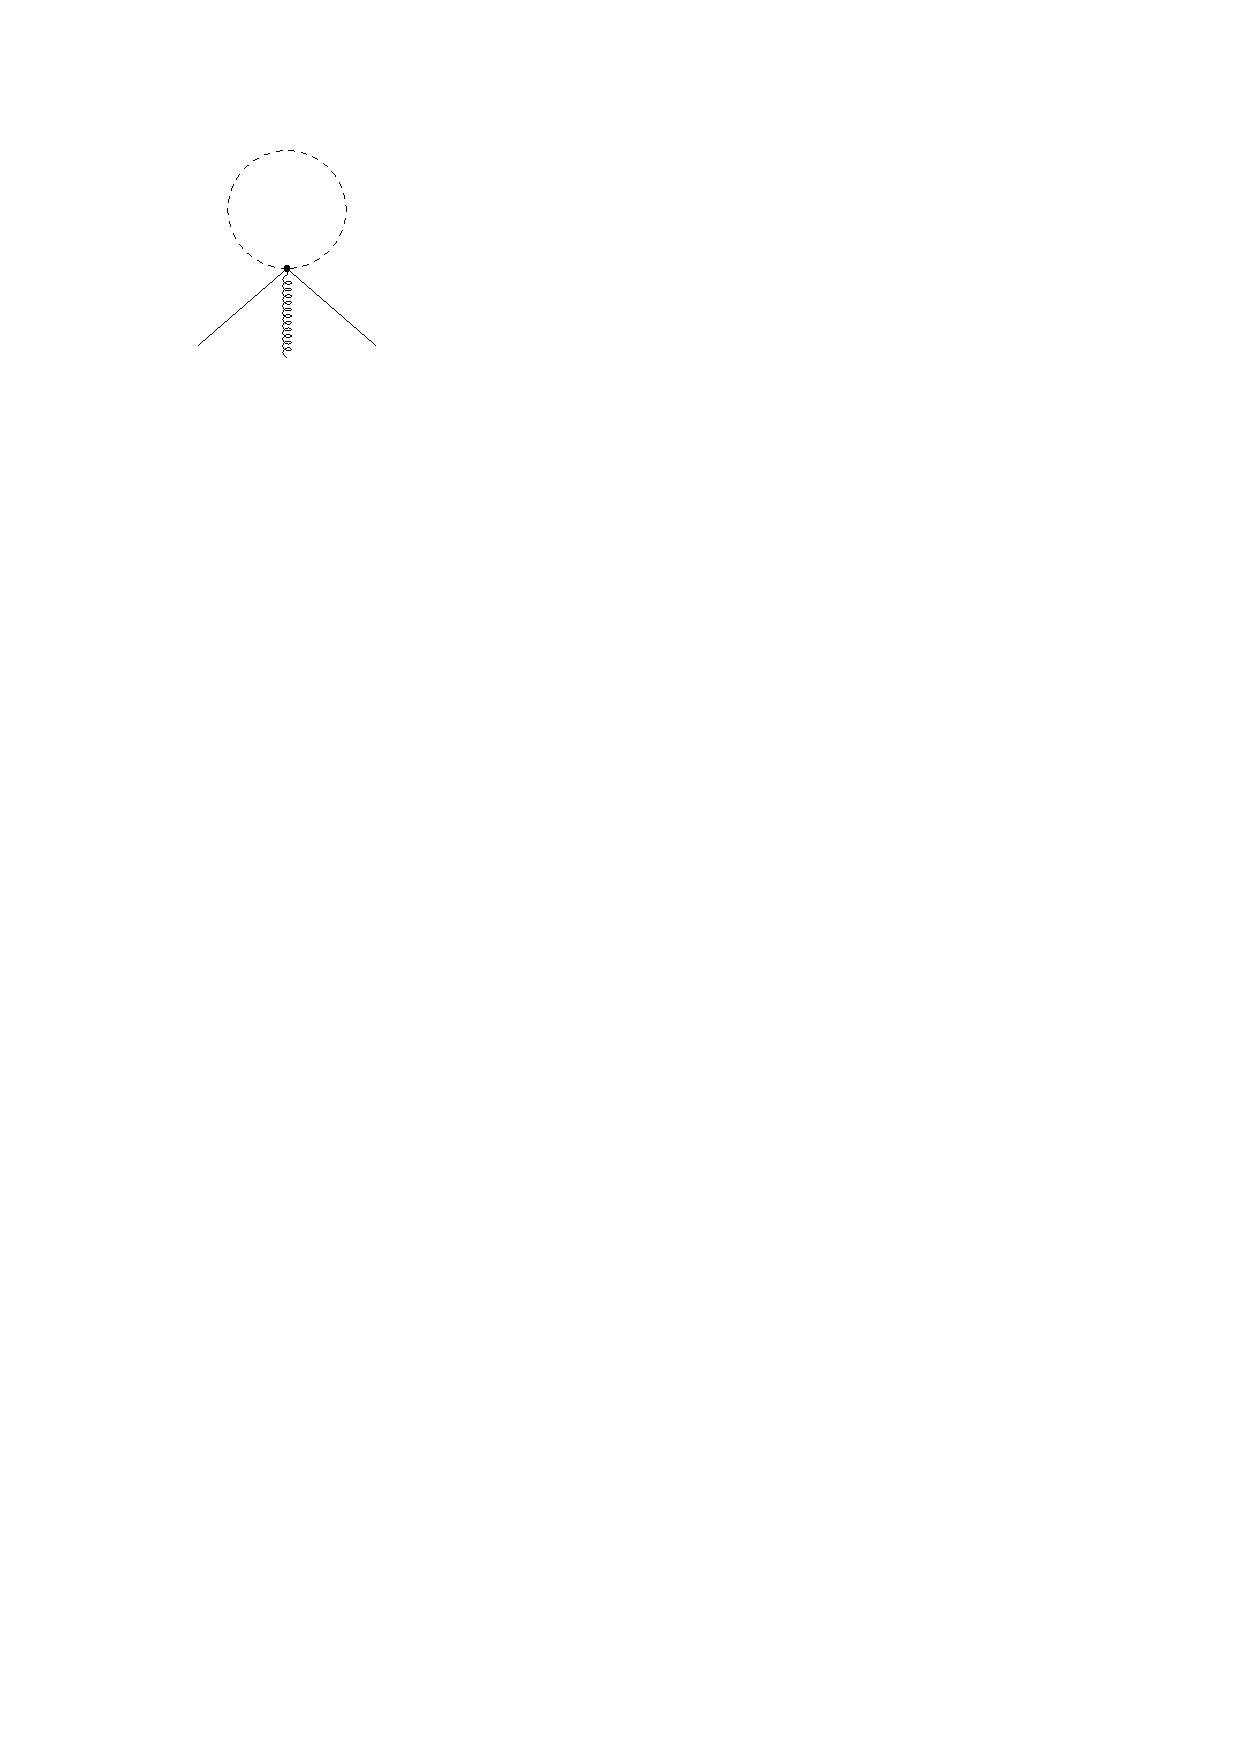
\includegraphics[width=0.33\linewidth,clip=true,trim=3cm 23cm 14cm 2cm]{5a.pdf}\quad 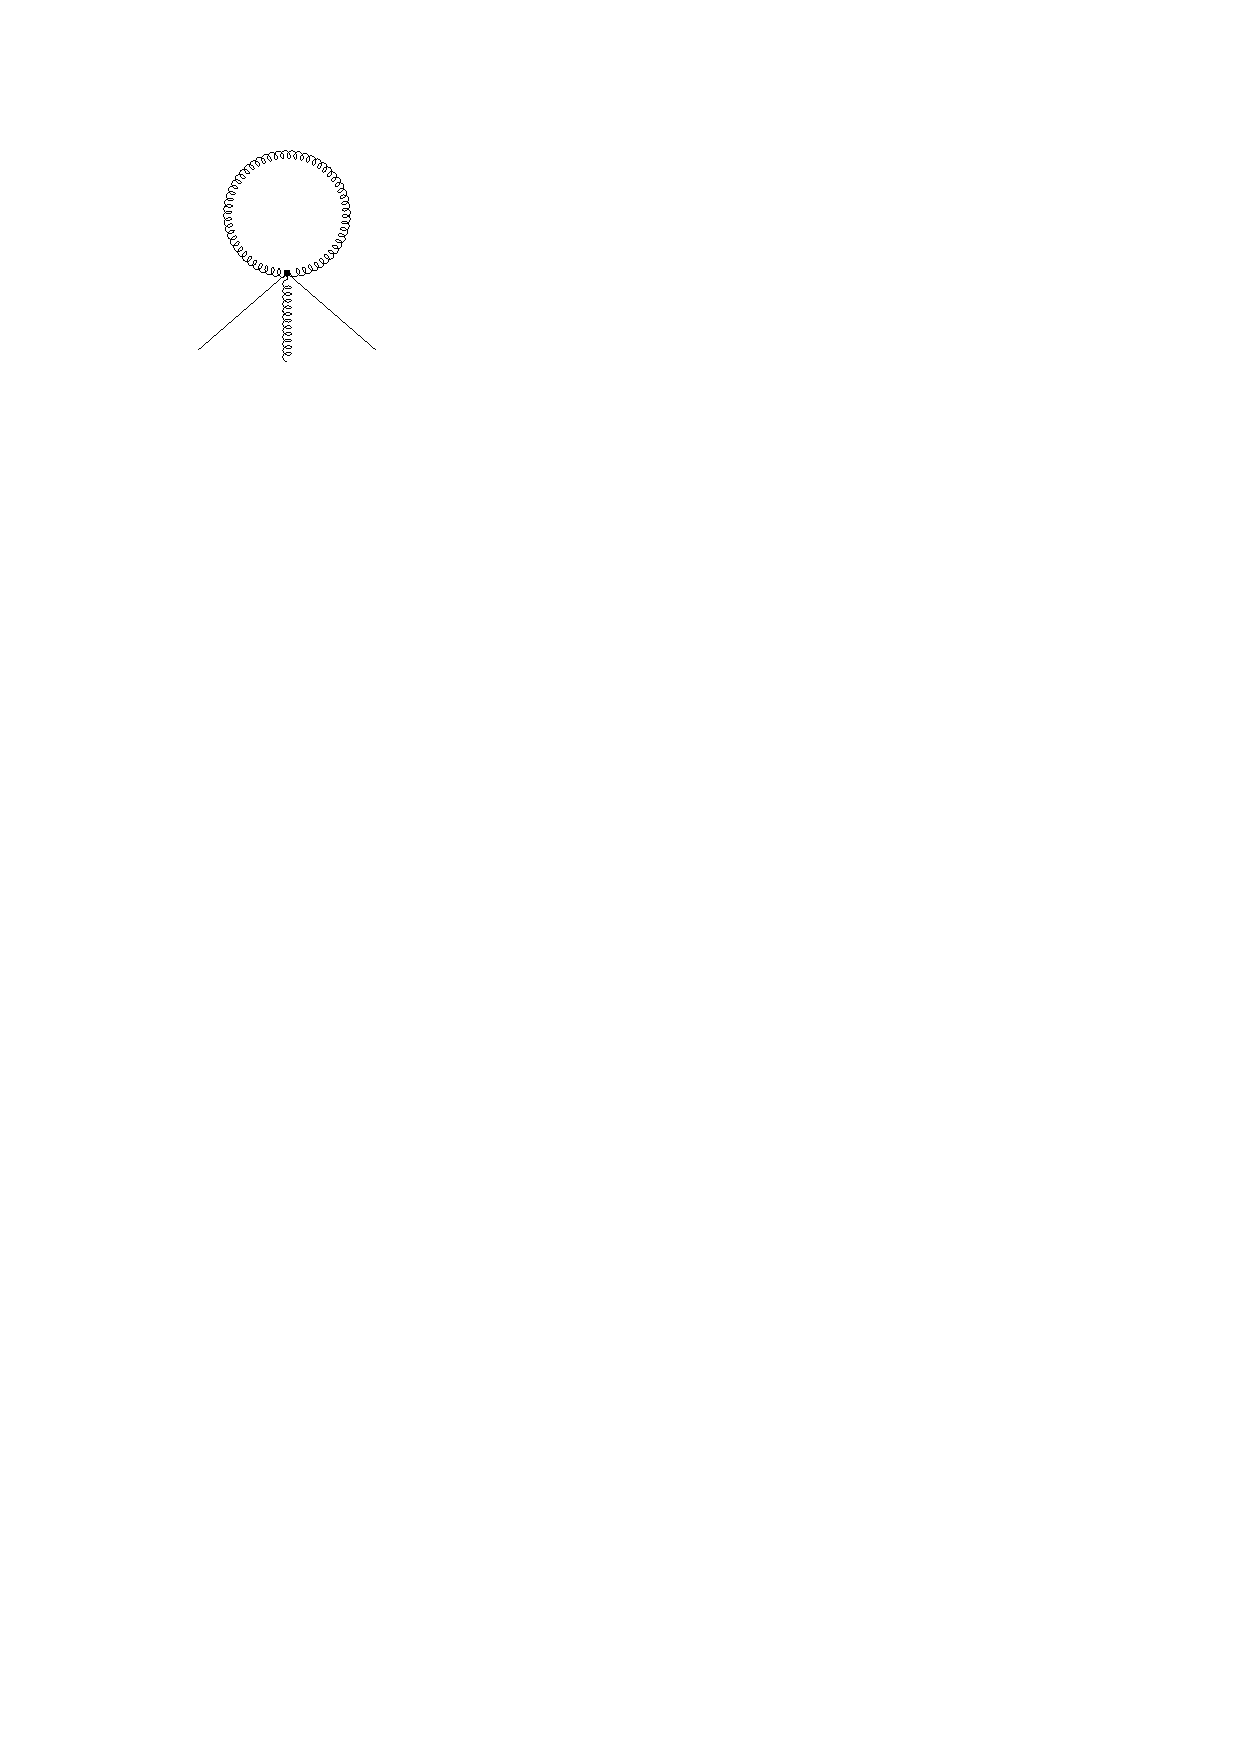
\includegraphics[width=0.33\linewidth,clip=true,trim=3cm 23cm 14cm 2cm]{5b.pdf}
\caption{\label{tadpolediags} Tadpole diagrams contributing to the flow of $\sqrt{g_3}$.
Each diagram features a regulator insertion on each of the internal propagators, which we omit here.
Curly lines denote the transverse traceless metric mode,
dashed lines the scalar graviton mode and continuous lines the scalar.}
\end{figure}

\begin{figure}
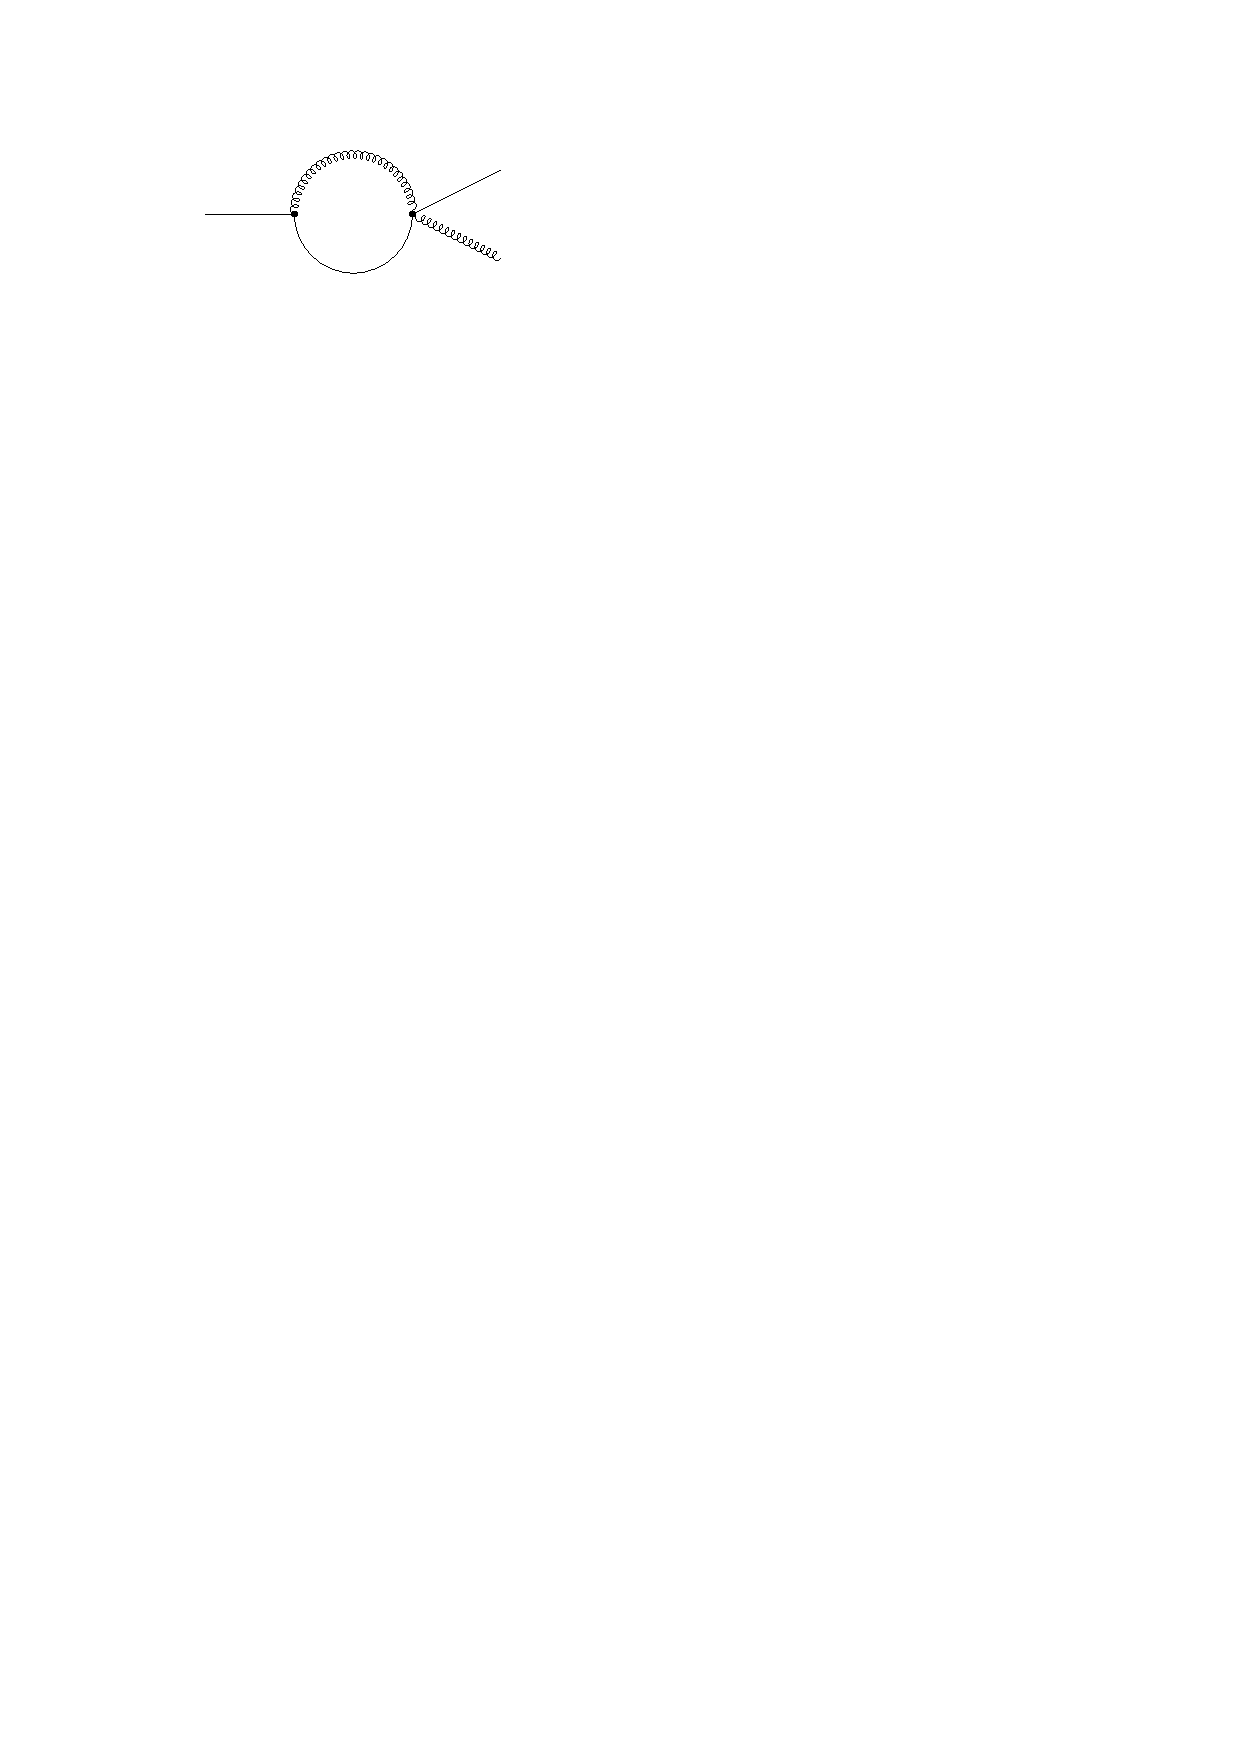
\includegraphics[width=0.45\linewidth,clip=true,trim=3cm 25cm 12cm 2cm]{3b.pdf}\quad
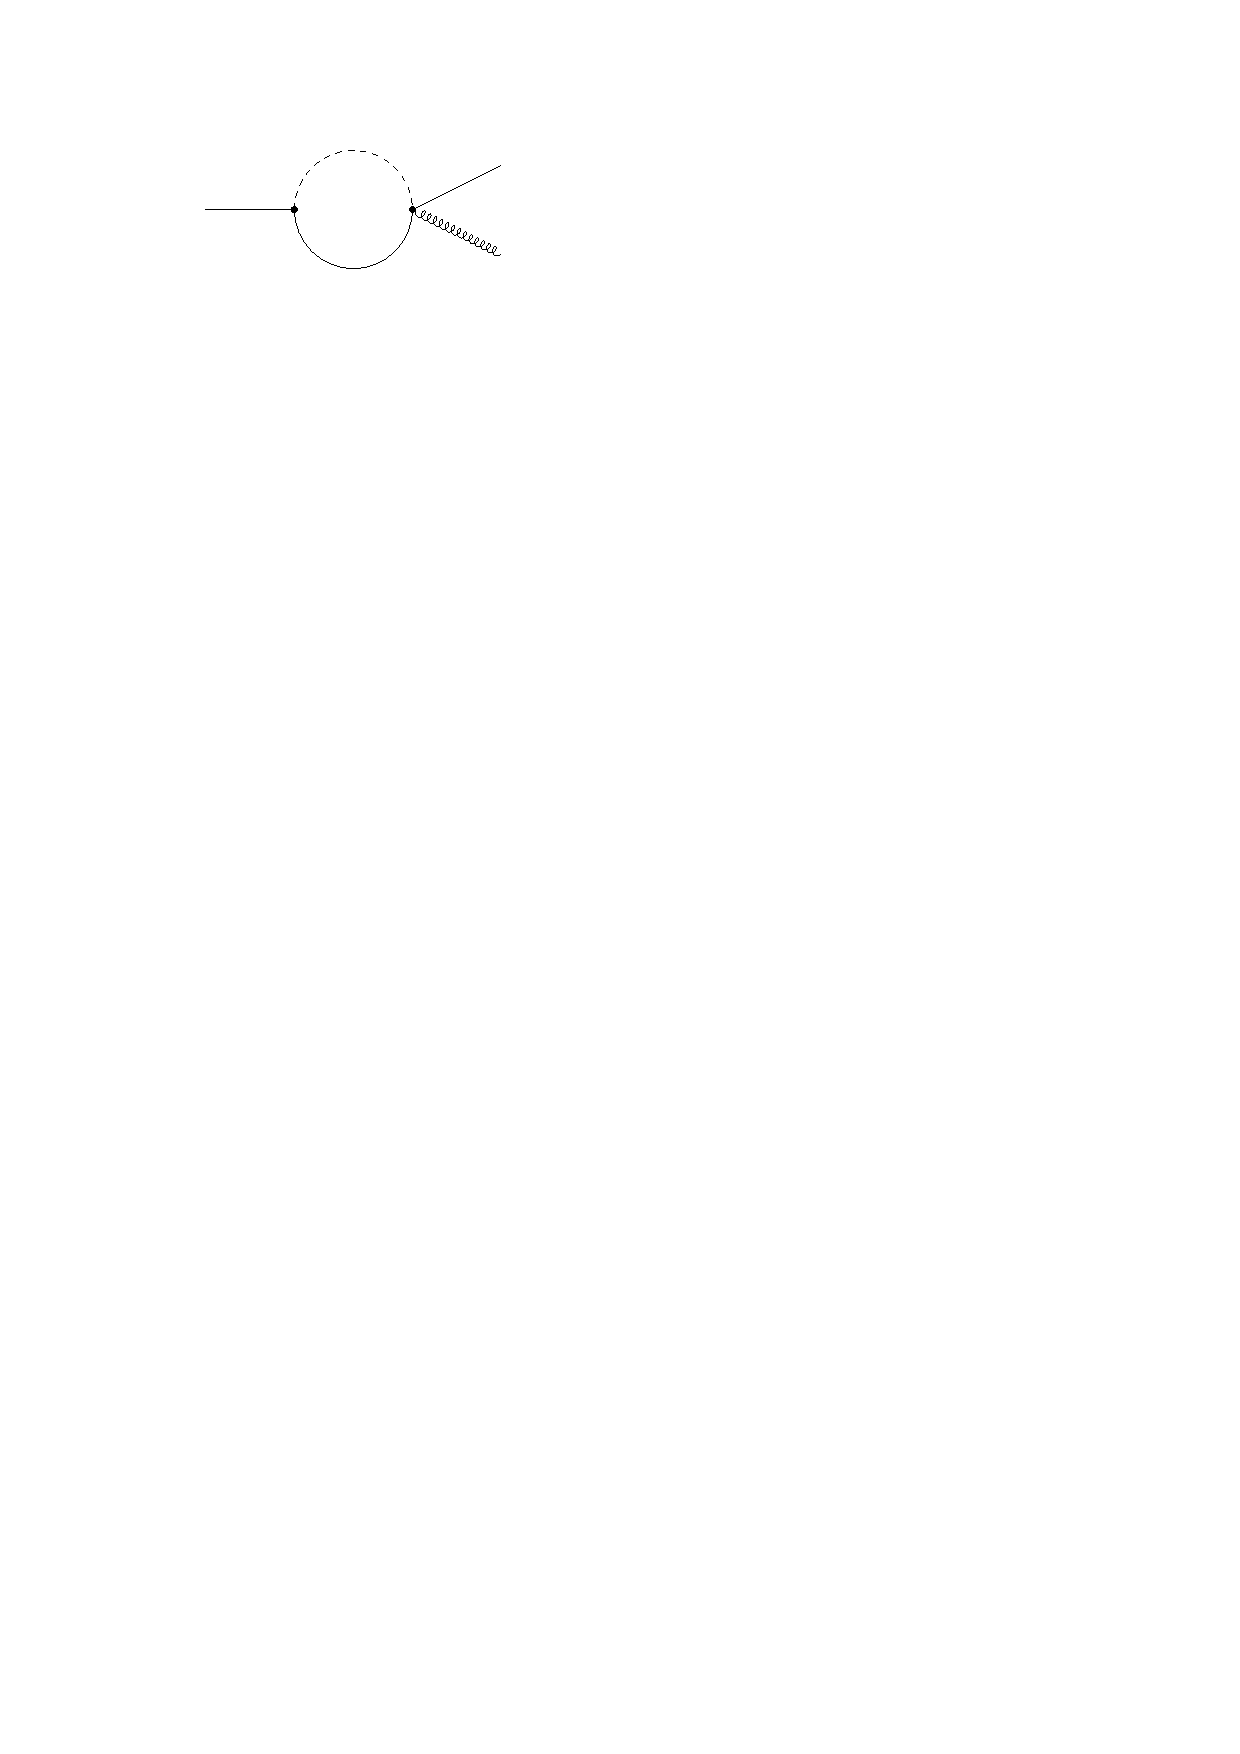
\includegraphics[width=0.45\linewidth,clip=true,trim=3cm 25cm 12cm 2cm]{3a.pdf}\newline
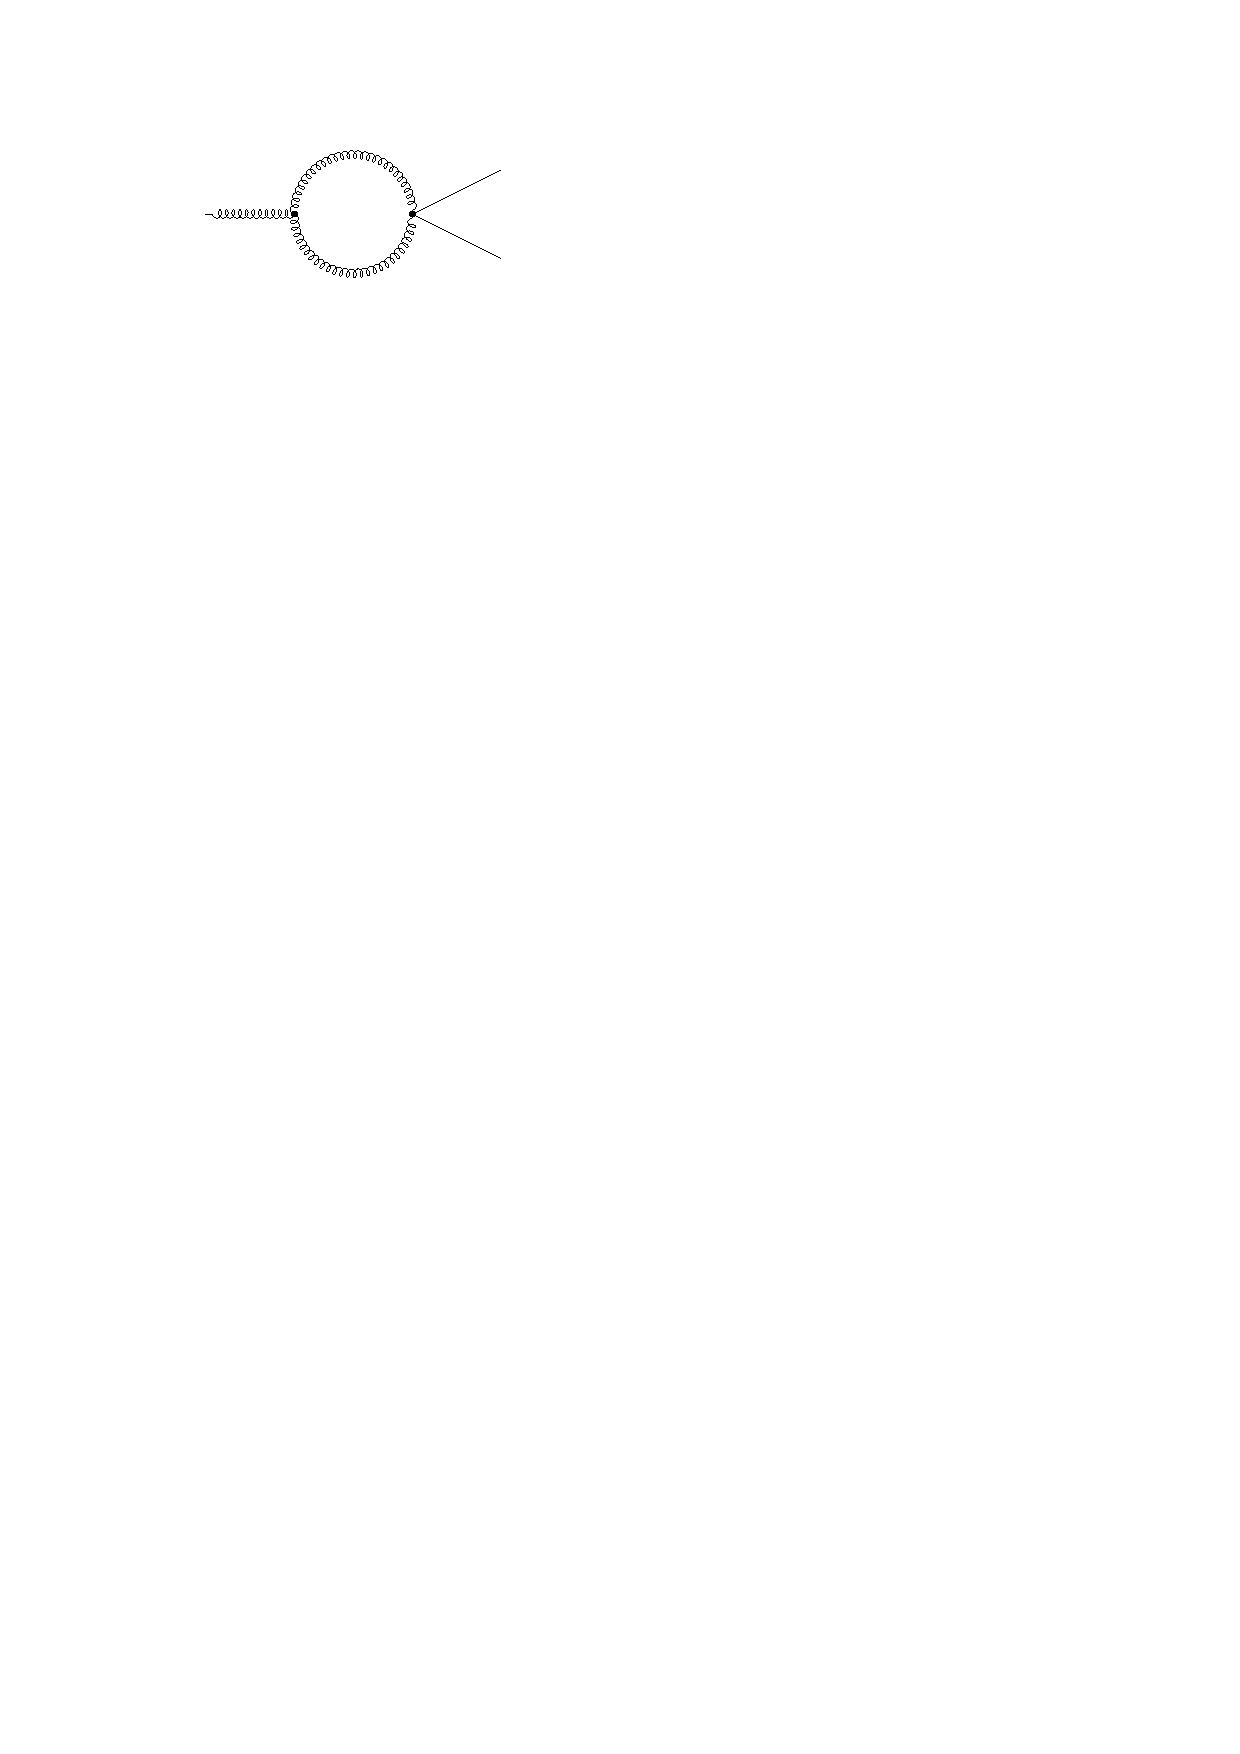
\includegraphics[width=0.45\linewidth,clip=true,trim=3cm 25cm 12cm 2cm]{4c.pdf}\quad
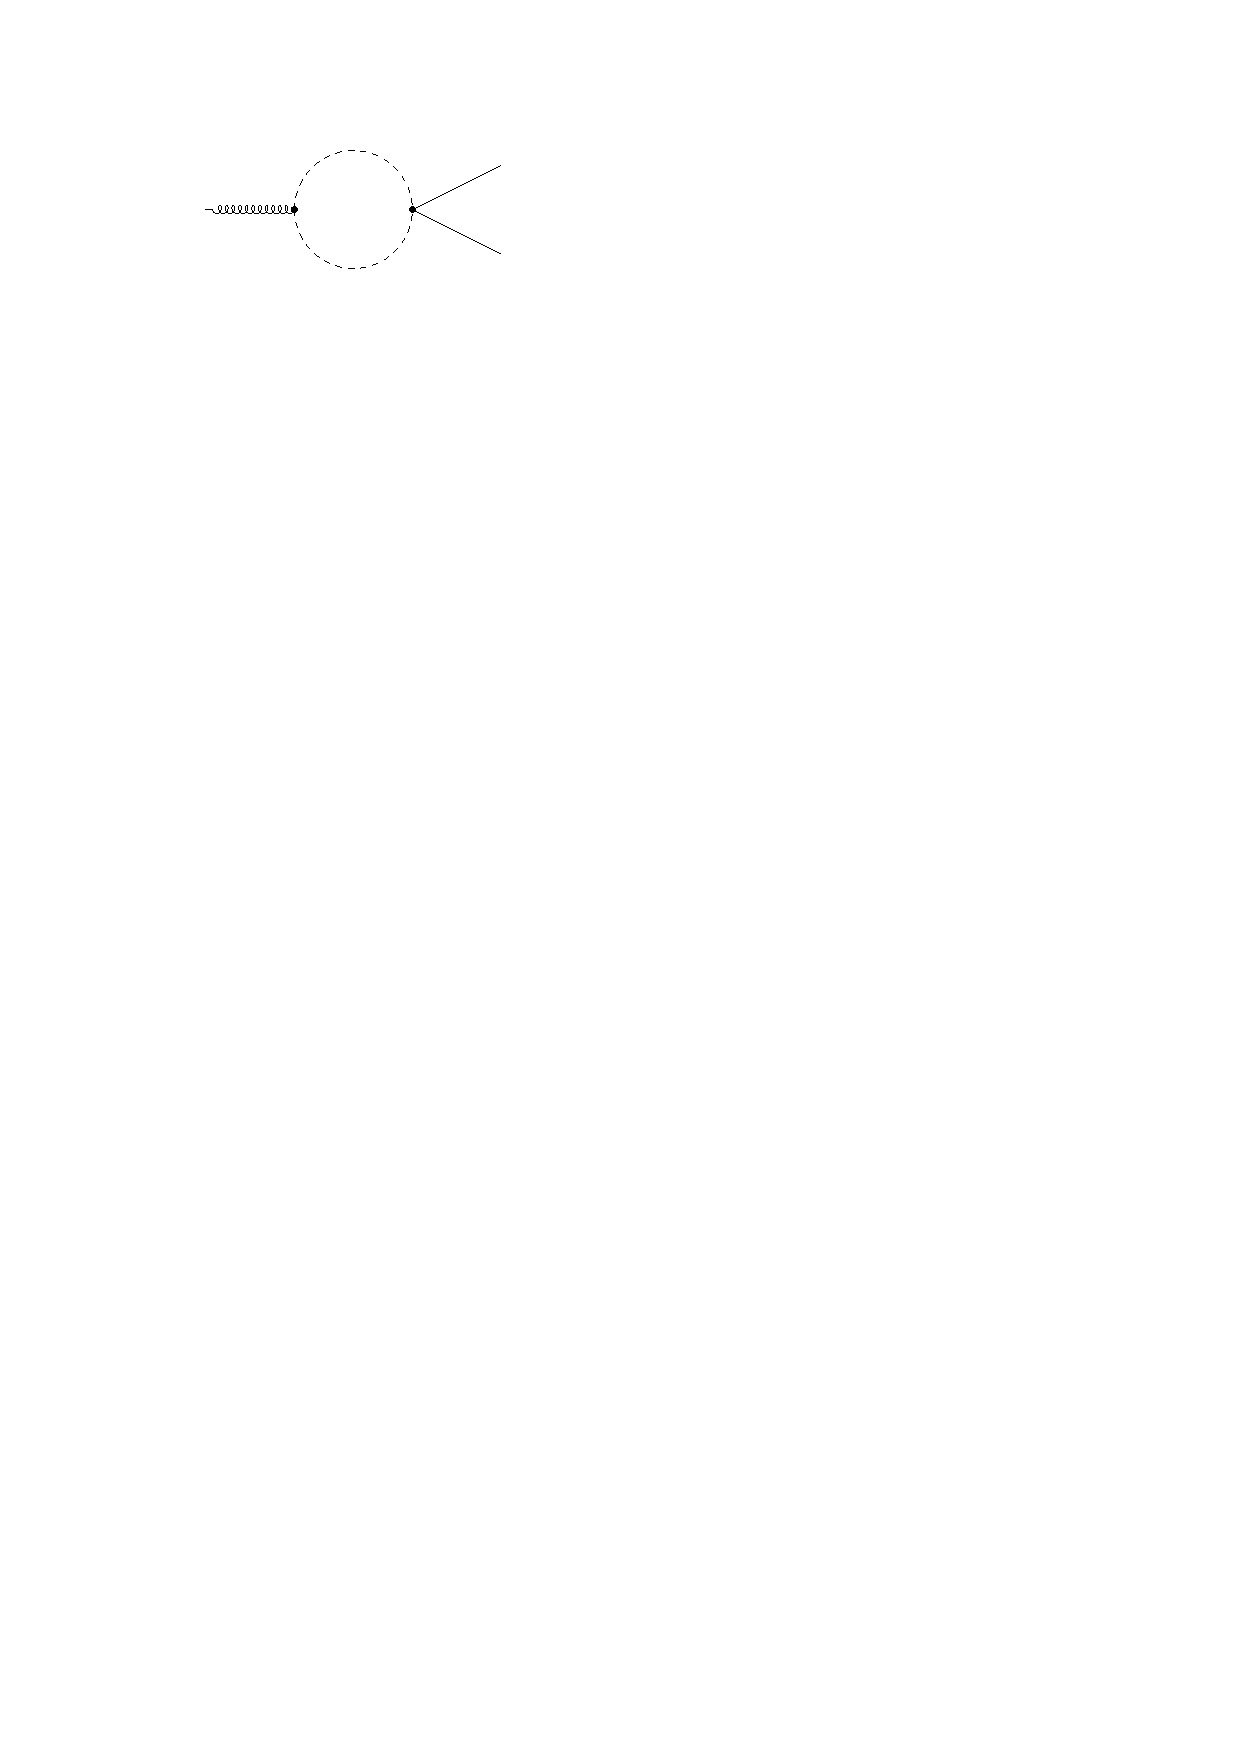
\includegraphics[width=0.45\linewidth,clip=true,trim=3cm 25cm 12cm 2cm]{4a.pdf}\quad
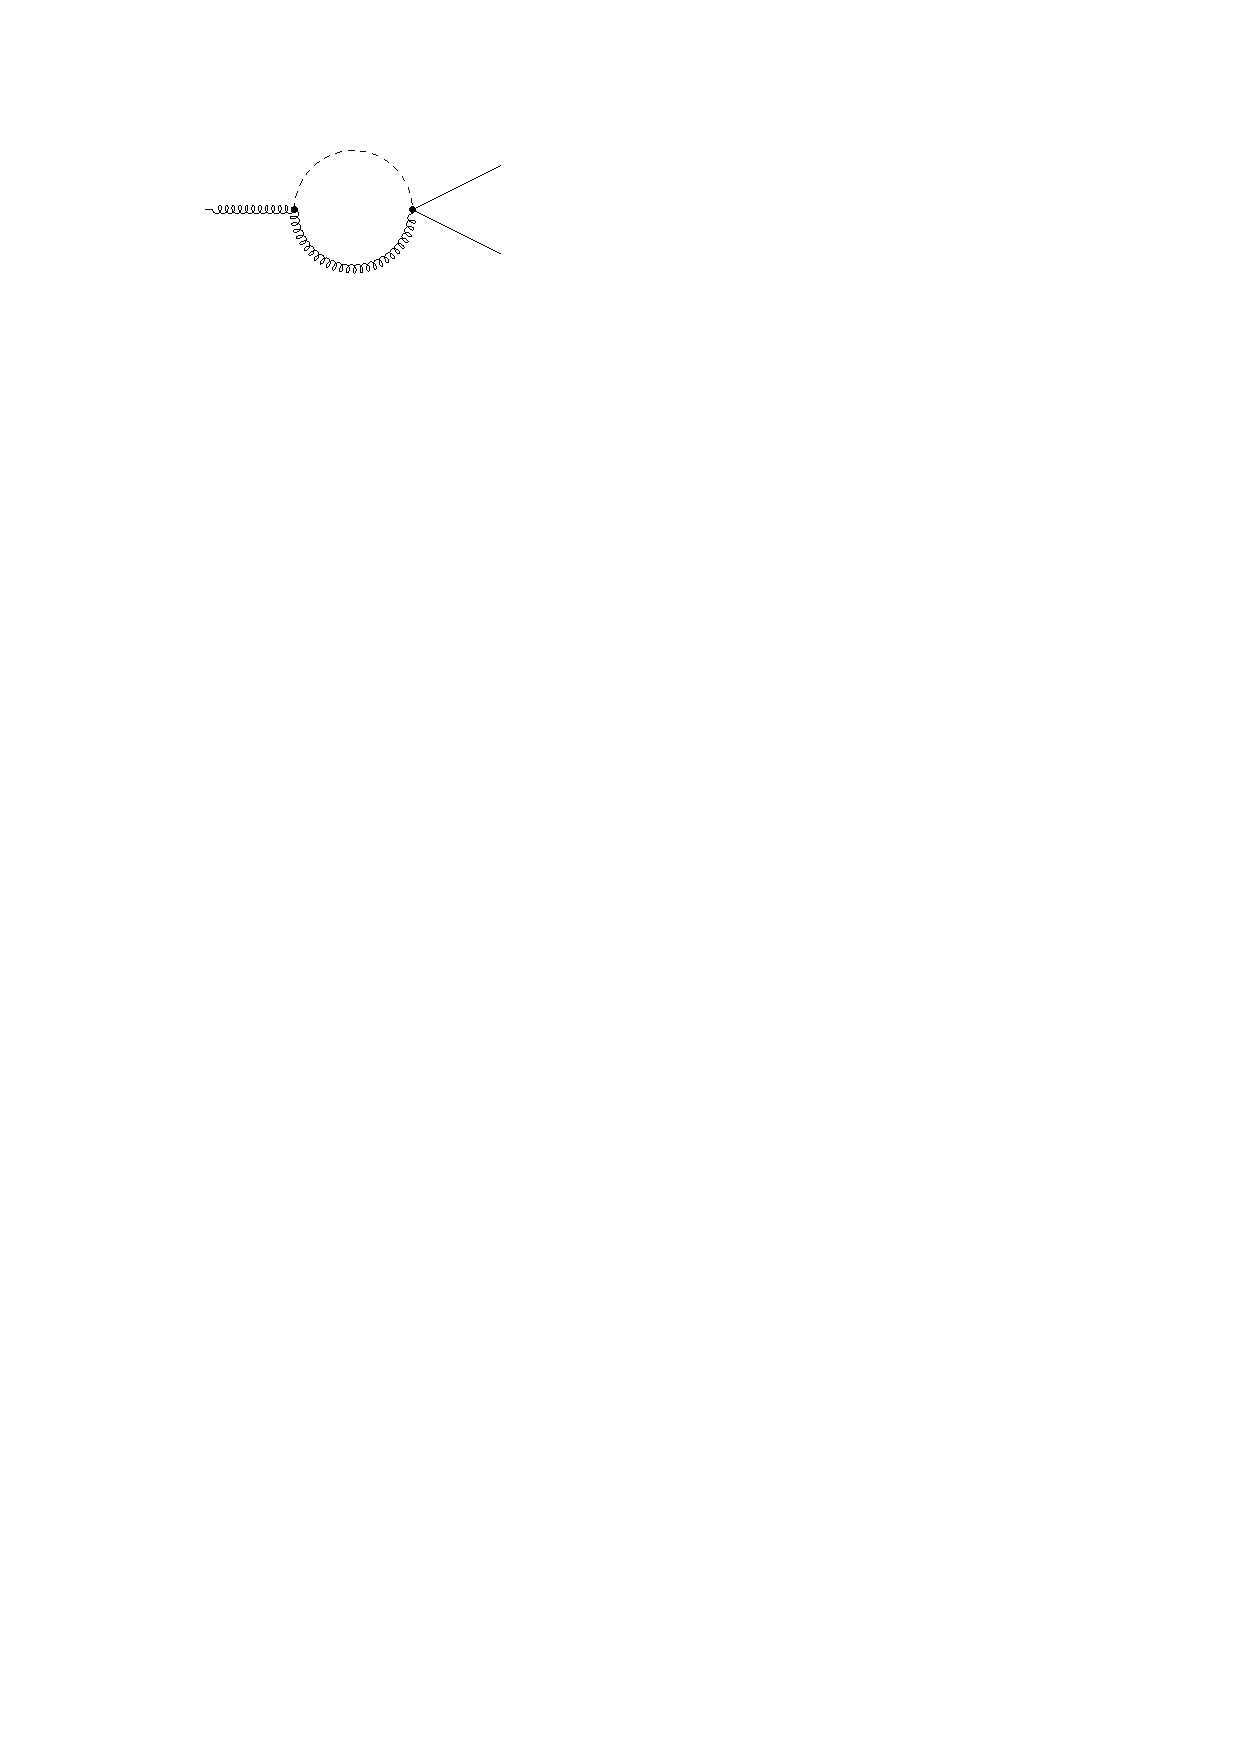
\includegraphics[width=0.45\linewidth,clip=true,trim=3cm 25cm 12cm 2cm]{4b.pdf}
\caption{\label{twovertexdiags} Two-vertex-diagrams contributing to the flow of $\sqrt{g_3}$.
Each diagram occurs in two versions with the regulator insertion appearing on each of the two internal
propagators in turn.Curly lines denote the transverse traceless metric mode,
dashed lines the scalar graviton mode and continuous lines the scalar.
The two diagrams in the first line feature only vertices that arise from the kinetic term for the scalar.
The other three diagrams also feature pure-metric vertices which arise from the Einstein-Hilbert action.}
\end{figure}

Additionally, there are tadpole diagrams and two-vertex diagrams,
which contain the couplings $g_4$ and $g_5^{3/2}$,
which also arise from the kinetic term of the scalar,
cf.~Fig.~\ref{tadpolediags} and Fig.~\ref{twovertexdiags}.
The two tadpole diagrams contribute at $\mathcal{O}(g_5^{3/2})$ to the flow of $g_3$.
Equation \eqref{TTtadpole} denotes the transverse traceless graviton contribution,
and \eqref{sigmatadpole} the scalar graviton contribution.
\bea
\beta_{\sqrt{g_3}}\Big|_{\rm TT\, tadpole} &=&
-\frac{95}{648 \pi}g_5^{3/2} \, (6-\eta_{\rm TT}),\label{TTtadpole}\\
\beta_{\sqrt{g_3}}\Big|_{\sigma \rm\, tadpole} &=&
\frac{19}{324 \pi} g_5^{3/2}\, (6-\eta_{\sigma}). \label{sigmatadpole}
\eea

The top two two-vertex diagrams in Fig.~\ref{twovertexdiags} contain only gravity-matter vertices,
and contributes at $\mathcal{O}(\sqrt{g_3} g_4)$ to the flow of $\sqrt{g_3}$:
\bea
\beta_{\sqrt{g_3}}\Big|_{\substack{\rm TT,\,S\\\rm two-vertex}}  &=& 0,\\
\beta_{\sqrt{g_3}}\Big|_{\substack{\rm \sigma,\,S\\\rm two-vertex}} &= &-\frac{5}{72 \pi} \sqrt{g_3} g_4 \, (16-\eta_{\sigma}-\eta_S).
\eea


Finally, there are two-vertex and three-vertex diagrams which also contain the vertex $\sqrt{G_3}$,
which arises from the Einstein-Hilbert action, cf.~Fig.~\ref{twovertexdiags}
and Fig.~\ref{threevertexdiags}.
The lower three diagrams in Fig.~\ref{twovertexdiags} yield
\bea
\beta_{\sqrt{g_3}}\Big|_{\substack{\rm TT,\,TT\\\rm two-vertex}}   &=& -\frac{5}{216 \pi}  g_4 \sqrt{G_3}\, (8-\eta_{\rm TT}),\\
\beta_{\sqrt{g_3}}\Big|_{\substack{\rm \sigma,\,\sigma\\\rm two-vertex}}   &= &-\frac{1}{54 \pi} g_4 \sqrt{G_3} \, (-8 + \eta_{\sigma}), \\
\beta_{\sqrt{g_3}}\Big|_{\substack{\sigma \rm,\,TT\\\rm two-vertex}}  &=& 0.
\eea


The three-vertex diagrams with a pure-gravity vertex, cf.~Fig.~\ref{threevertexdiags},
yield the following contribution:

\bea
\beta_{\sqrt{g_3}}\Big|_{\substack{\sigma,\,\sigma,\,S \rm \\ \rm 3-vertex}} &=&\!\!\frac{1}{80\pi}g_3 \sqrt{G_3} \, (30-2\eta_{\sigma}-\eta_S),\\
\beta_{\sqrt{g_3}}\Big|_{\substack{\rm TT,\,TT,\,S\\ \rm 3-vertex}} &=& 0, \\
\beta_{\sqrt{g_3}}\Big|_{\substack{\sigma,\,\rm TT,\,S\\ \rm 3-vertex}} &=& 0.\label{threevertexpuregravityvertex}
\eea

\begin{figure}
\centering
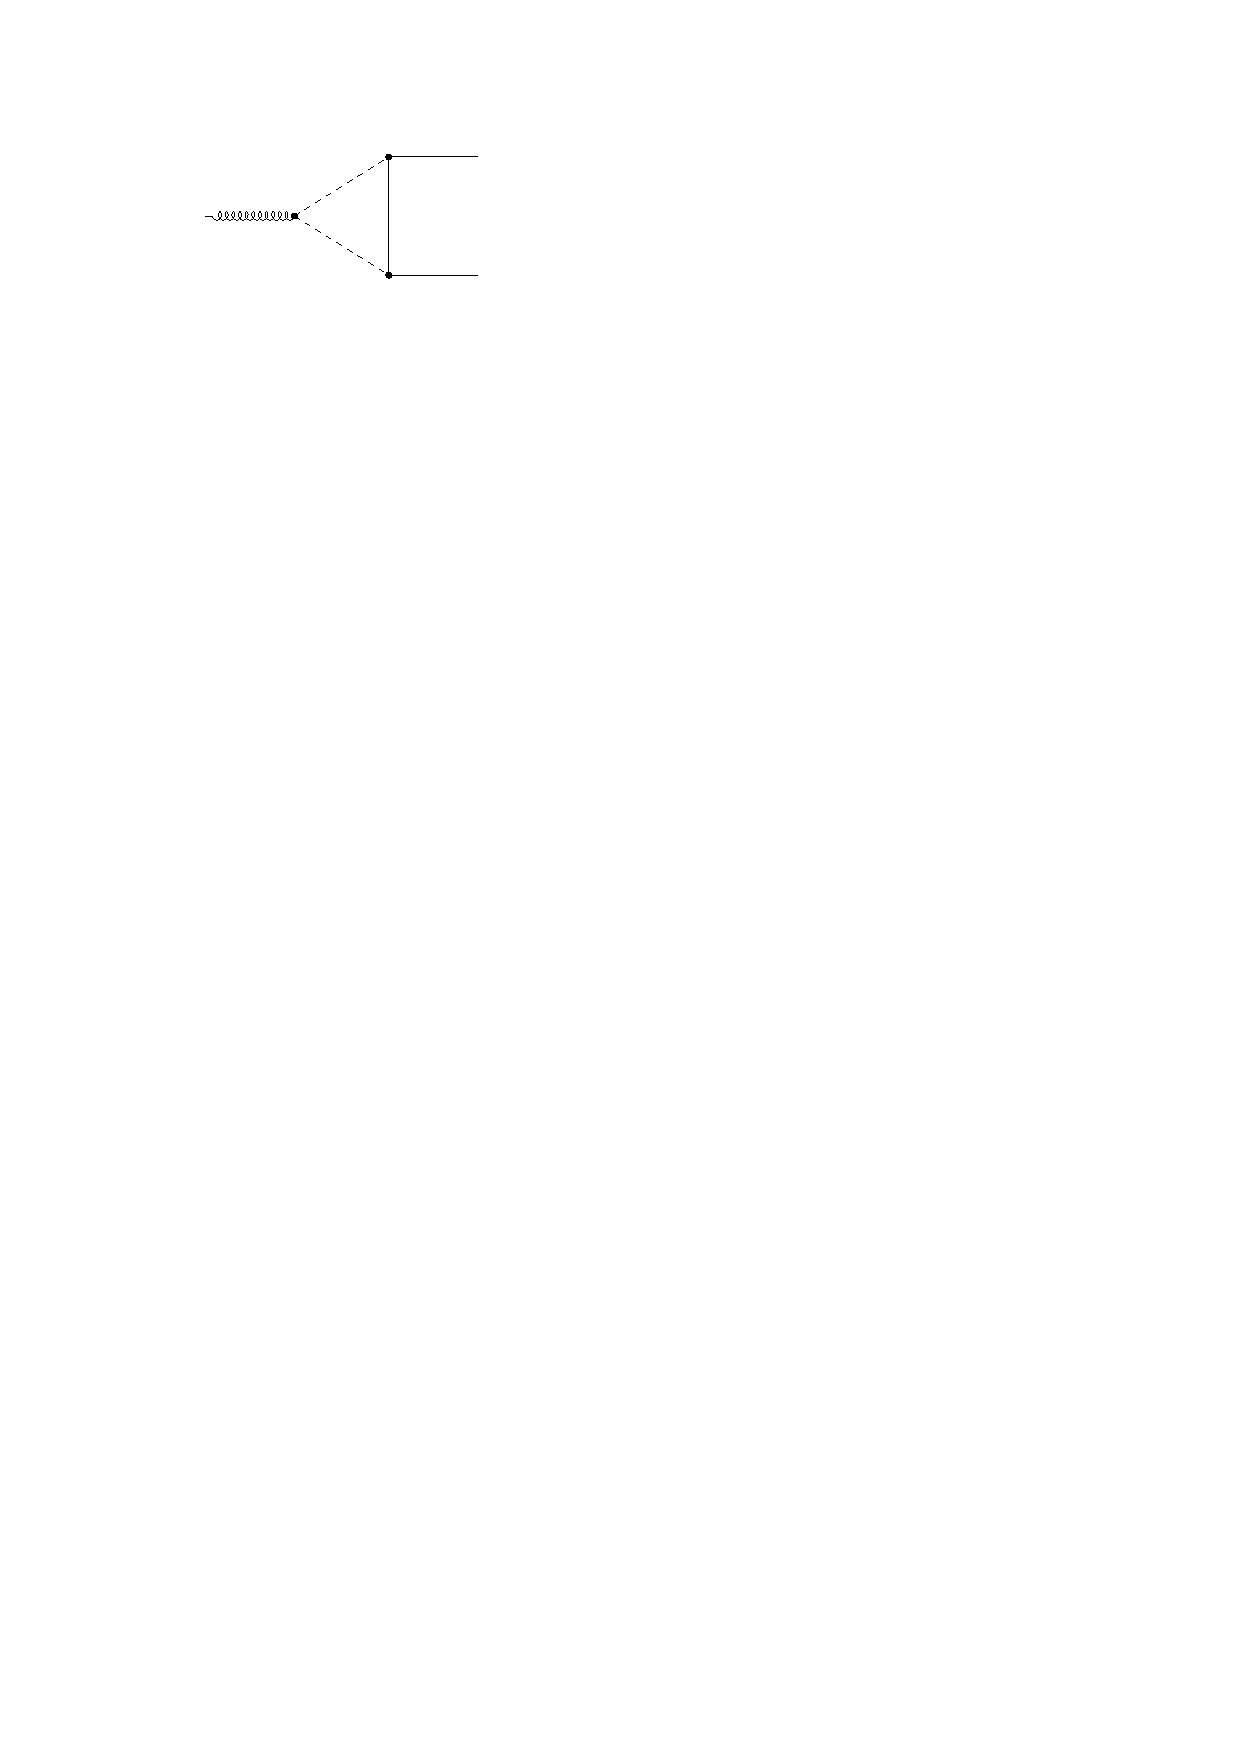
\includegraphics[width=0.45\linewidth,clip=true,trim=3cm 25cm 12cm 2cm]{2c.pdf}
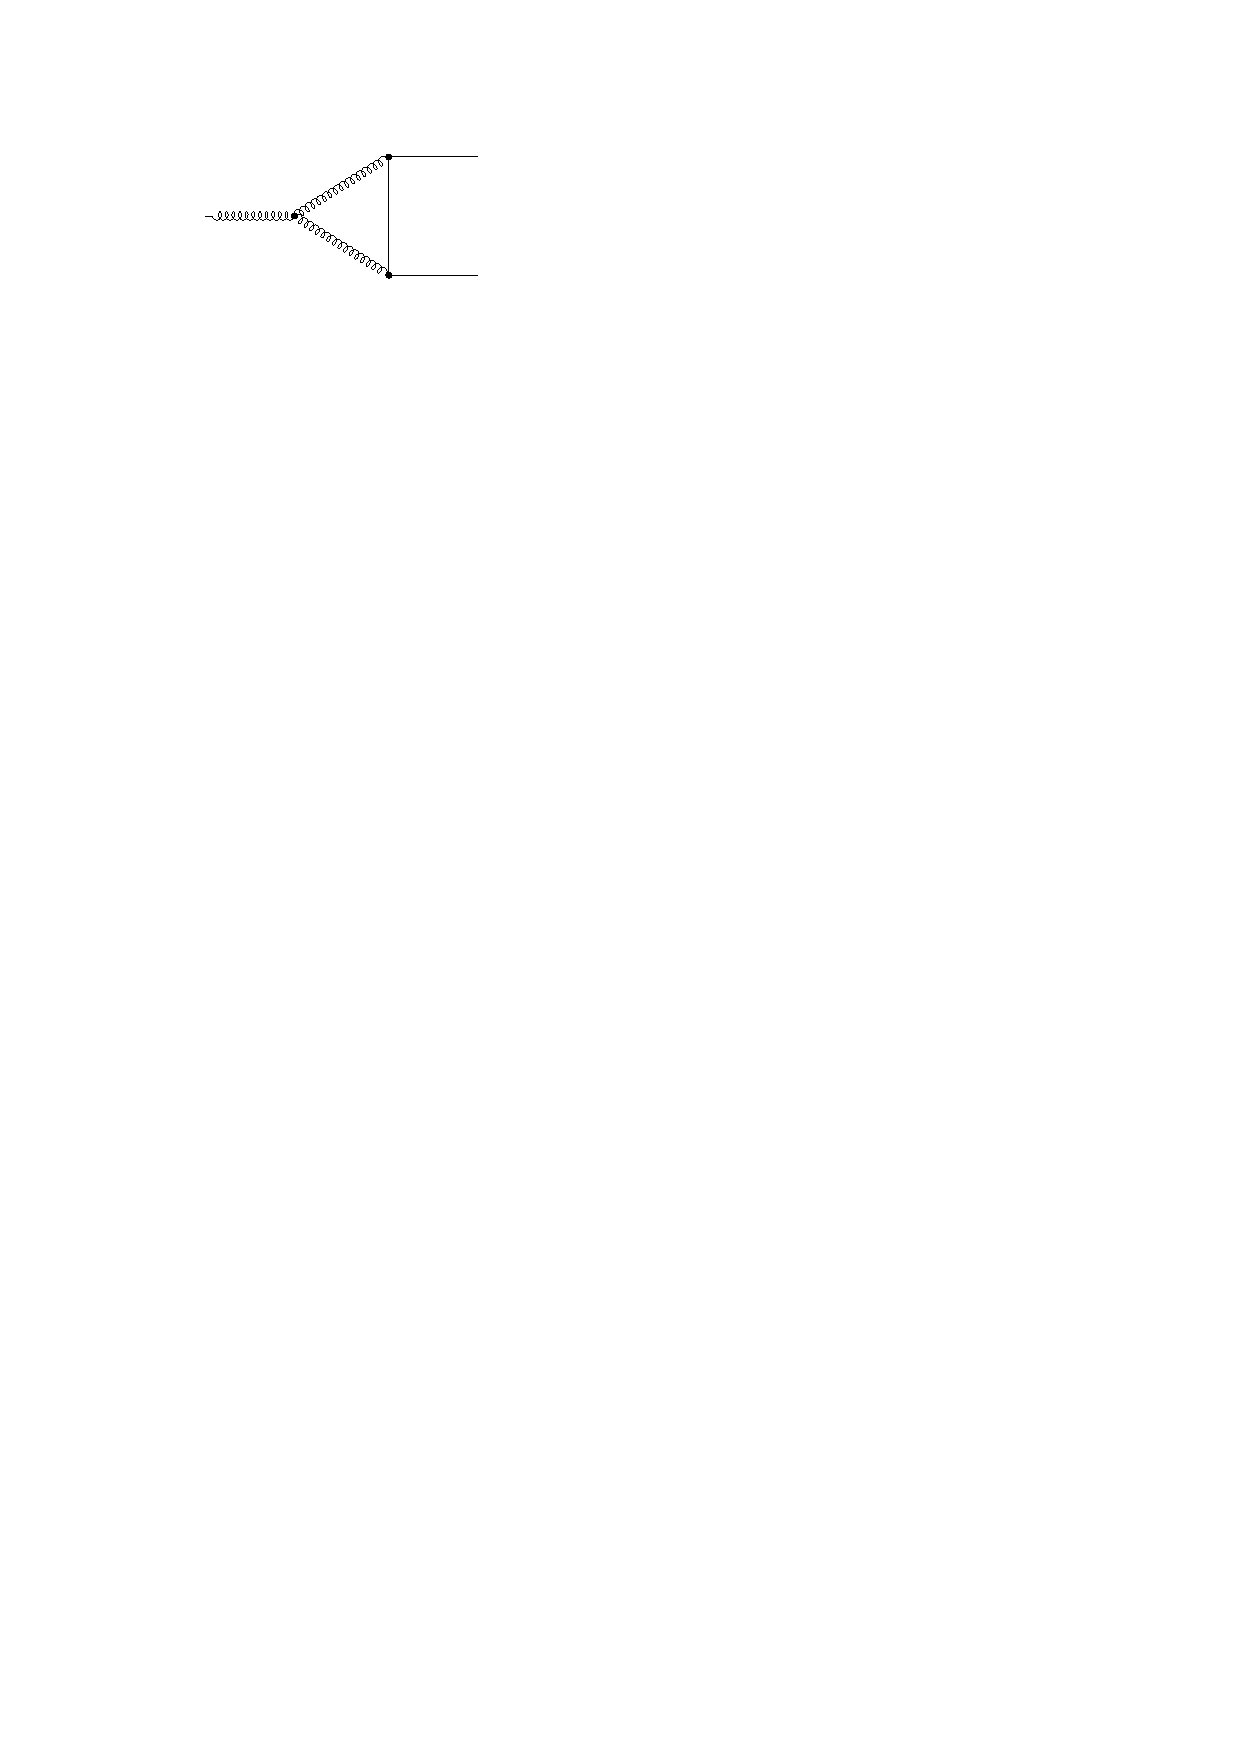
\includegraphics[width=0.45\linewidth,clip=true,trim=3cm 25cm 12cm 2cm]{2a.pdf}\newline
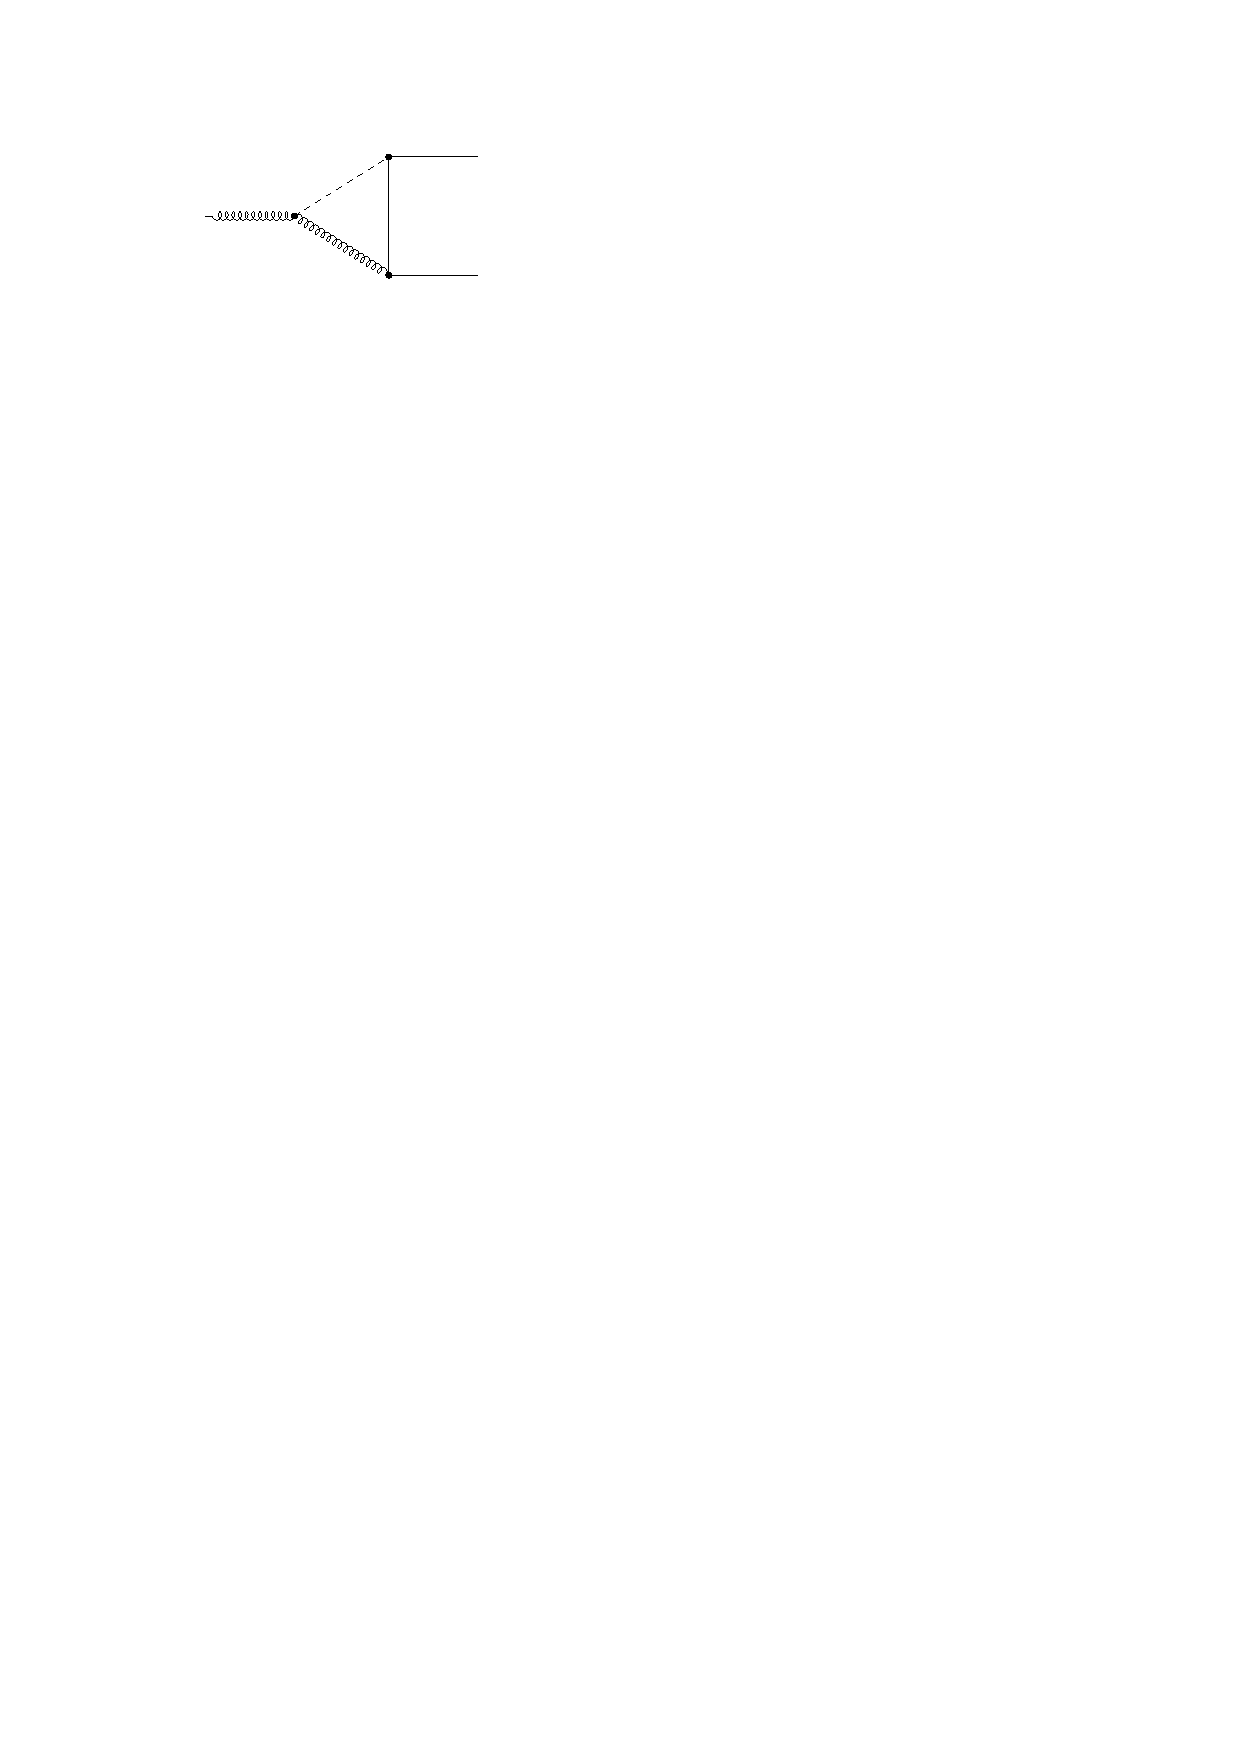
\includegraphics[width=0.45\linewidth,clip=true,trim=3cm 25cm 12cm 2cm]{2b.pdf}
\caption{\label{threevertexdiags} Three-vertex-diagrams contributing to the flow of $\sqrt{g_3}$,
which also feature a pure-gravity vertex.
Each diagram occurs in three versions with the regulator insertion appearing on each of the three
internal propagators in turn. Curly lines denote the transverse traceless metric mode,
dashed lines the scalar graviton mode and continuous lines the scalar.}
\end{figure}


%%
\subsection{Beta function for $g_3$}
%%
By summing Eq.~\eqref{betag3threevertexg3} to Eq.~\eqref{threevertexpuregravityvertex} we
obtain the beta function for $\sqrt{g_3}$,
from which we derive the beta function for the dimensionless $g_3$ as
%
\bea
\beta_{g_3}& =&
\left(2+\eta_{\rm TT}+2\eta_S\right)g_3
+\frac{3}{4\pi}g_3^2
+ \frac{3}{4\pi}g_3^{3/2}\sqrt{G_3}
\nonumber\\
&-&\!\frac{20}{9\pi}g_3 g_4
- \frac{2}{3 \pi} \sqrt{g_3}\sqrt{G_3}g_4
- \frac{19}{18 \pi} g_5^{3/2}\sqrt{g_3}
\nonumber\\
&+& \!\left(\frac{5}{108\pi}g_4 \sqrt{G_3}
+ \frac{95}{324\pi} g_5^{3/2}\right)\sqrt{g_3}\eta_{\rm TT}
\nonumber\\
&+&\! \!\Bigl(-\frac{1}{40 \pi}g_3^{3/2}
- \frac{1}{20 \pi} g_3 \sqrt{G_3}
+ \frac{5}{36 \pi} \sqrt{g_3} g_4
\nonumber\\
&{}&+ \frac{1}{27 \pi}g_4 \sqrt{G_3}
- \frac{19}{162\pi}g_5^{3/2}\Bigr)\sqrt{g_3}\eta_{\sigma}
%\nonumber
\\
&+& \!\left(- \frac{1}{20 \pi}g_3^{3/2}
- \frac{1}{40 \pi} g_3 \sqrt{G_3}
+ \frac{5}{36 \pi}\sqrt{g_3} g_4 \right)\sqrt{g_3}\eta_S.
\nonumber%\\
%&{}&\label{betag3result}
\eea
%
Herein, the factors $\eta_{\rm TT} g_3$ and $2 \eta_S g_3$ appear if the kinetic terms of both
fields are redefined with a canonical prefactor,
and the corresponding factors of the wave-function renormalization are absorbed in the coupling $g_3$.

 There is a significant difference to other possible definitions of a running Newton coupling:
 the beta function of $g_3$ depends implicitly on $N_S$,
 since only $\eta_{TT}$ and $\eta_{\sigma}$ contains a $N_S$ dependence.
There is no pure matter-loop contributing to $\beta_{g_3}$, though,
as there is for some other definitions of a running Newton coupling, e.g.,
for the background Newton coupling \cite{Dona:2013qba},
or for the pure-gravity coupling $G_3$ \cite{Meibohm:2015twa}.


%%
\section{Results for the pure gravity case}
%%
Let us now analyze the fixed-point structure within various approximations.
If we consider the scalar as an external field, and only integrate out metric fluctuations,
we can still consider $g_3$ as our definition of the running Newton coupling.
In that case $\beta_{g_3}$ is determined by the tadpole diagrams in
Fig.~\ref{tadpolediags} and the last three diagrams in Fig.~\ref{twovertexdiags}.
The anomalous dimensions only receive contributions from the diagrams in Fig.~\ref{etahdiagsgrav}
that do not contain matter in the loops.
They can be obtained from the general formulas simply putting $N_S=0$.
Here we further put the anomalous dimension $\eta_S$ to zero.

If we then employ the approximation $g_5 = g_4 = g_3$, $G_3 = G_4 = g_3$, we obtain
\be
\beta_{g_3}= (2+\eta_{TT})g_3
- \frac{31}{18 \pi}g_3^2
+\frac{55}{162\pi}g_3^2\eta_{TT}
-\frac{13}{162\pi}g_3^2\eta_\sigma
\ee
where
\bea
\eta_{TT}&=&\frac{2g_3(1591 g_3-55296 \pi)}{2665 g_3^2-3384\pi g_3 +124416 \pi^2}
\\
\eta_\sigma&=&\frac{2g_3(16195 g_3+32832 \pi)}{2665 g_3^2-3384\pi g_3 +124416 \pi^2}
\eea

We  define the semi-perturbative approximation by setting
$\eta_{\rm TT}= \eta_{\sigma}=\eta_S = 0$ on the right-hand sides of all diagrams contributing
to the flow of the $\eta$'s.
Then $\eta_{\rm TT}$ and $\eta_S$ still appear on the right-hand side of $\beta_{g_3}$.
This semi-perturbative approximation removes potential poles from $\beta_{g_3}$ that are
due to the nonperturbative structure of the $\eta$'s, and which could induce artificial zeros.
In this approximation
\bea
\beta_{g_3}= 2g_3 - \frac{47}{18 \pi}g_3^2
-\frac{223}{648\pi}g_g^3.\label{purgravitysemipertbeta}
\eea
This structure, in particular the negative sign in front of the term $\sim g_3^2$,
is similar to that found for other definitions of the Newton coupling.

The interplay between the dimensional term $2g_3$ and the leading order term from quantum fluctuations,
$- g_3^2$, induces one real interacting fixed point as given in Tab.~\ref{puregravityFP_table}.
The semi-perturbative approximation features another real fixed point,
which we discard as a truncation artefact, as it is not present in the full beta function.
Moreover, the perturbative approximation, in which we set all anomalous dimensions to zero everywhere,
yields a similar result, where the critical exponent is of course set exactly by the negative dimensionality
of the coupling.

\begin{table}[]
  \begin{center}
    \begin{tabular}{ l r r r r }
      \toprule
      approximation      & $g_{3\,\ast}$ & $\theta$ & $\eta_{\rm TT}$ & $\eta_{\sigma}$ \\
      \midrule
      full               & 2.204         & 2.17     & -0.62           & 0.50 \\
      semi-perturbative  & 2.203         & 2.17     & -0.62           & 0.37 \\
      perturbative       & 3.65          & 2        & -               & -    \\
      \bottomrule
    \end{tabular}
  \end{center}
  \caption{
    Coordinates and critical exponents at an interacting fixed point for vanishing scalar fluctuations.
    In the perturbative approximation we have set $\eta_{\rm TT}=\eta_{\sigma}=0$.
  }
  \label{puregravityFP_table}
\end{table}

The real part of the critical exponent is remarkably close to values in previous approximations,
both in the single- and bi-metric case. We emphasize that this is a  rather non-trivial result.
In our case, we define a coupling $g_3$, which is related to a gravity-scalar interaction vertex,
in contrast to previous pure-gravity definitions.
Accordingly, the diagrams entering the beta function have a fairly different structure,
as does the beta function.
It is rather reassuring to note that different ways of defining a Newton coupling and projecting
the RG flow onto it result in similar universal properties.

The relatively large fixed-point value for $g_3$ is clearly responsible for the large absolute
values of the anomalous dimensions, as $\eta \sim g_{3\,\ast}$: For instance,
if we set $g_3=1$ by hand, we obtain $\eta_{\rm TT} = -0.28$ and $\eta_{\sigma} =0.20$.
It has been observed previously that the exponential parameterization features a large fixed-point
value for the Newton coupling in the single-metric approximation \cite{Percacci:2015wwa},
and our definition of the fluctuation-field coupling exhibits similar behavior.

The large negative value for the TT anomalous dimension suggests a propagator that decays with a
higher power of the momentum in the UV, potentially suppressing the effect of TT quantum
fluctuations in the UV.
On the other hand, the positive value for the scalar anomalous dimension implies that the
$\sigma$ mode is actually enhanced in the UV.
In particular, this could have very interesting consequences for gravity-operators at the UV fixed point.
Operators of more ``scalar character" would be shifted towards relevance by the positive anomalous
dimension $\eta_{\sigma}$, while operators with a larger contribution to the transverse traceless sector
would be shifted towards irrelevance, even if the canonical dimension of both operators agrees.
In particular, this could suggest that more complicated tensor structures,
such as, e.g., powers of the Ricci tensor or Riemann tensor could be less relevant than their
Ricci scalar counterparts.
(This concurs with an observation made in \cite{Codello:2006in}.)


Interestingly, the sign of $\eta_{\rm TT}$ is opposite to results in the
linear parametrization \cite{Codello:2013fpa, Dona:2013qba, Christiansen:2014raa}.
If we identify $\eta_{\sigma} = \eta_{\rm TT}$ we obtain a fixed point with the properties
listed in Tab.~\ref{puregravityFPetaapprox}.
We observe a comparable value for the critical exponent $\theta$ with  respect to the previous case.
The anomalous dimension for the TT mode remains essentially the same.
We see that the assumption $\eta_{\sigma}=\eta_{TT}$ even gives the wrong sign for $\eta_\sigma$.
Since the anomalous dimensions contribute to the scaling dimensions of operators,
this is of course a serious shortcoming.

\begin{table}[]
  \begin{center}
  \begin{tabular}{ l r r r }
    \toprule
    approximation     & $g_{3\,\ast}$ & $\theta$ & $\eta_{\rm TT}$ \\
    \midrule
    full              & 2.20          & 2.19     & -0.67 \\
    semi-perturbative & 2.26          & 2.12     & -0.64 \\
    \bottomrule
  \end{tabular}
  \end{center}
  \caption{
    Coordinates and critical exponents of an interacting fixed point with the
    approximation $\eta_{\sigma} = \eta_{\rm TT}$.
  }
  \label{puregravityFPetaapprox}
\end{table}

To test the stability of our results with respect to extended truncations which would include separate
beta functions for $G_3$ etc.,
we consider an approximation where $g_5=g_4=g_3$.
We treat the pure-gravity coupling $G_4=G_3$ as an external parameter,
and test whether a viable fixed point exists for values of these couplings between 0 and 6.
For this case, we display the semi-perturbative result, as it allows a clear understanding of the terms:
\bea
\beta_{g_3} &=&2 g_3 - \frac{8}{9 \pi} g_3 G_3
- \frac{19}{18 \pi}g_3^2
\\
&{}& - \frac{209 g_3^2 G_3}{648 \pi^2}
- \frac{2}{3 \pi}g_3^{3/2}\sqrt{G_3}
- \frac{7}{324 \pi^2}g_3^{3/2}G_3^{3/2}\ .
\nonumber
\eea
When $G_3$ increases, the fixed point for $g_3$ decreases, cf.~Fig.~\ref{puregravityFP}.
We see that the fixed point that we have observed in the approximation $G_3=g_3$,
persists for a large range of values of $G_3$.
We interpret this as a sign of stability.

\begin{figure}
  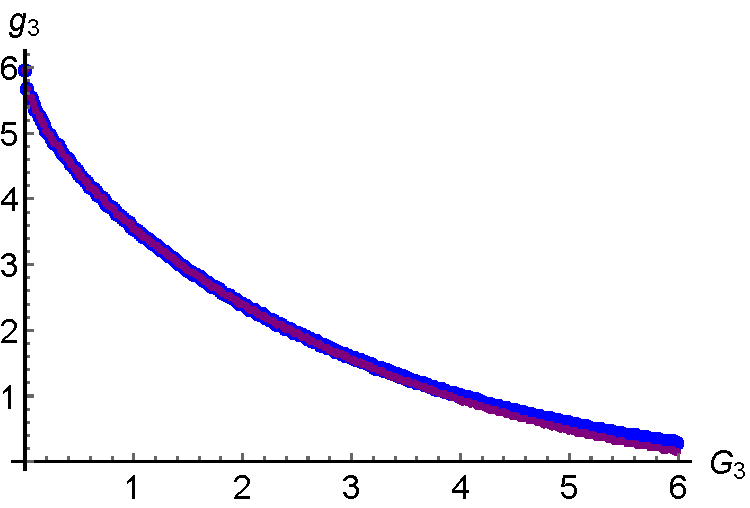
\includegraphics[width=\linewidth]{g3_G3_puregravity.pdf}\\
  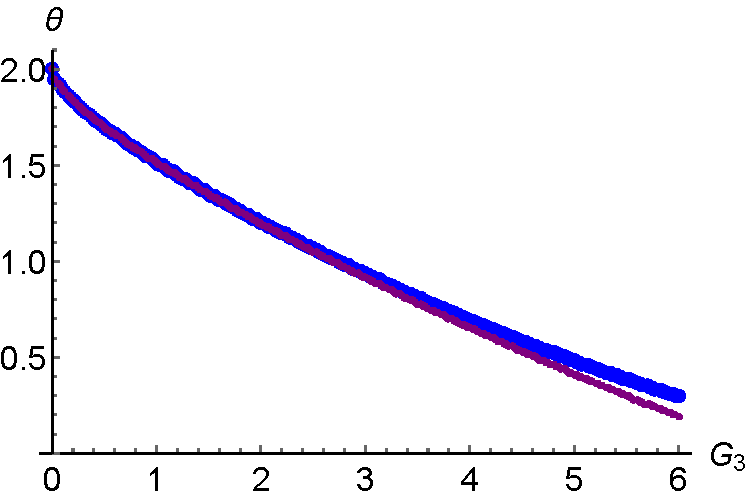
\includegraphics[width=\linewidth]{theta_G3_puregravity.pdf}
  \caption{\label{puregravityFP} We show the fixed point value for $g_3$ (upper panel)
    and the critical exponent $\theta$ (lower panel) as a function of $G_3=G_4$.
  The larger blue dots denote the full result and the smaller purple dots the semi-perturbative approximation.}
\end{figure}

\begin{figure}
  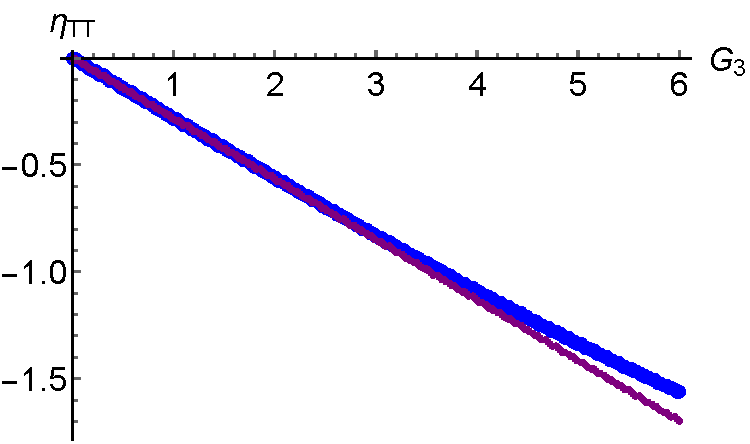
\includegraphics[width=0.45\linewidth]{etah_puregravity.pdf}\quad
  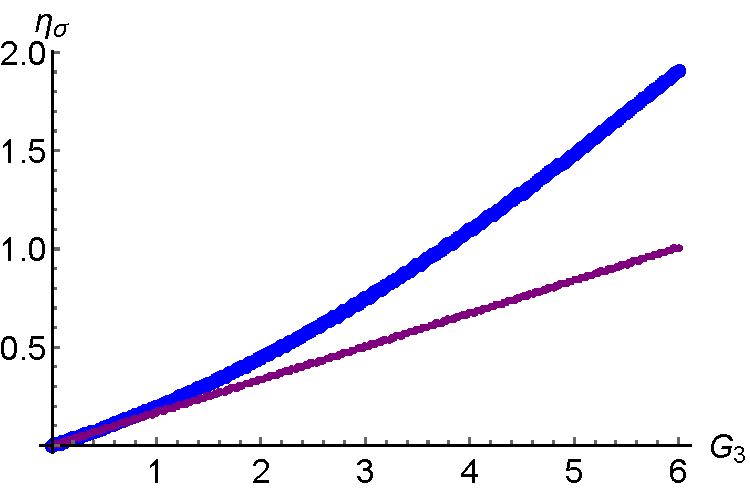
\includegraphics[width=0.45\linewidth]{etasigma_puregravity.pdf}
  \caption{\label{puregravityeta}We show the fixed point value for $\eta_{\rm TT}$ (left panel)
  and $\eta_{\sigma}$ (right panel) as a function of $G_3=G_4$.
The larger blue dots denote the full result and the smaller purple dots the perturbative approximation.}
\end{figure}

Fig.~\ref{puregravityeta} shows the anomalous dimensions at the fixed point as functions of $G_3$.
Note that they vanish for $G_3=0$, since, in the absence of matter self interactions, they are
generated only by diagrams proportional to $G_3$.
 Note that to obtain this result, the identification $g_5=g_3$,
 suggested by diffeomorphism invariance, is crucial,
 as it gives rise to the above structure of the beta function.

The critical exponent $\theta$ in this approximation is not equal to the result of
Tab.~\ref{puregravityFP_table} at $G_3=g_3$,
since $\partial \beta_{g_3}/\partial G_3 \vert_{G_3=g_3}$ contributes to the critical
exponent quoted in that table. When we distinguish $g_3$ and $G_3$,
then  $\partial \beta_{g_3}/\partial G_3 \vert_{G_3=g_3}$ yields an \emph{off-diagonal} contribution
to the stability matrix, which can contribute to the critical exponents if operators mix
at the non-Gau\ss{}ian fixed point. As we only evaluate the diagonal entry of the stabilty
matrix in our approximation, where $G_3$ is treated as an external parameter, that contribution is absent.


We now supplement our beta functions by a beta function for the background Newton coupling,
as obtained in \cite{Percacci:2015wwa}, where
\be
\beta_{\bar{G}}=2 \bar{G} - \frac{\bar{G}^2}{\pi} \left(\frac{15}{8}- \frac{5 \eta_{\rm TT}}{18 }+ \frac{\eta_{\sigma}}{24} \right).
\ee
We observe that $\eta_{\rm TT}$ and $\eta_{\sigma}$ enter with the opposite sign.
At the fluctuation-field fixed point, $\eta_{\rm TT}<0$  and $\eta_{\sigma}>0$.
This sign combination strengthens the gravitational fluctuation effects that induce a fixed point,
lending further support to the observation that all modes of the graviton act towards asymptotic
safety \cite{Reuter:2008qx, Reuter:2008wj}.

Plugging in the fluctuation field fixed point-values---which are of course independent
of $\bar{G}$, as they should---we obtain $\bar{G}_{\ast} = 3.04$ and $\theta=2$.


%%%%%%%%%%%%%%%%%%%%%%%%%%%%%%%%%%%%%%%%%%%%%%%%%%%%%%%%%%%
\section{Results for the interacting matter-gravity system}
%%%%%%%%%%%%%%%%%%%%%%%%%%%%%%%%%%%%%%%%%%%%%%%%%%%%%%%%%%%
In the following, we switch on scalar fluctuations,
which adds several classes of diagrams to $\beta_{g_3}$ and additional contributions to
$\beta_{g_3}$, $\eta_{\rm TT}$ and $\eta_{\sigma}$.
Our main goal is to find out whether the pure-gravity results discussed above can be
extended in a stable way to $N_S>0$,
or whether scalars have a significant effect on the fixed point in our approximation.
First, we will set $\eta_S=0$ by hand, while taking into account $\eta_{\rm TT}$ and $\eta_{\sigma}$.
The reason for this unequal treatment of fluctuation fields will become clear below.

%
\subsection{Fixed-point results without scalar anomalous dimension}
%
As a first approximation, we set $G_3=G_4=g_4=g_5=g_3$,
and find an extension of the pure-gravity fixed point to $N_S>0$.
Unlike the beta functions for the background Newton coupling and the pure-gravity
couplings $G_3$ and $G_4$, $\beta_{g_3}$ receives no correction from diagrams containing
a scalar loop  in our approximation.
Consequently, $\beta_{g_3}$ does not depend on $N_S$ explicitly, if we set all anomalous dimensions to zero.
It only depends on $N_S$ if we include the anomalous dimensions $\eta_{\rm TT}$ and $\eta_{\sigma}$.
This gives rise to a beta function of the form
\be
\beta_{g_3}= 2g_3 -\frac{1}{3\pi}g_3^2\left(10-\frac{N_S}{8}\right)
+\mathcal{O}(g_3^3).
\label{norma}
\ee
Herein, the factor $10/3\pi$ differs from the  factor $47/18\pi$ in
Eq.~\eqref{purgravitysemipertbeta} since it includes contributions form scalar fluctuations
which do not scale with $N_S$.
In our determination of fixed points we also take into account all higher-order terms,
but the main effect of scalars is clear from the $\mathcal{O}(g_3^2)$ term:
As the contribution of scalars, that scales with $N_S$ explicitly,
comes with the opposite sign from the asymptotic safety-inducing term which enters with $-10g_3^2/3\pi$,
scalars push the fixed-point of $g_3$ towards larger values.
This is the same effect that we have already observed for the background-system \cite{Dona:2013qba}.
Interestingly, the contribution of scalars to the running of the three-graviton coupling features
an opposite sign in the approximation used in \cite{Meibohm:2015twa}.
On the other hand, the complete fixed-point dynamics in \cite{Meibohm:2015twa} is similar,
as $G_{3\,\ast}$ is also pushed to larger values,
since destabilizing effects of scalars show up in the momentum-independent part of the
graviton-three- and two-point function.


In our approximation, the fixed point merges with another,
artificial fixed point at $N_S\approx 28$, where the fixed point disappear into the complex plane,
cf.~Fig.~\ref{g3Nsnoetas}.
While this could indicate the existence of a bound on $N_S$ in asymptotically safe gravity,
we note that $\eta_{\sigma}>2$ already at $N_S=14$,
indicating that a larger truncation is required to investigate that regime in more detail,
see \cite{Meibohm:2015twa}. In the semi-perturbative approximation,
the anomalous dimensions are slightly smaller,
and the fixed-point collision accordingly occurs at larger $N_S$.

\begin{figure}
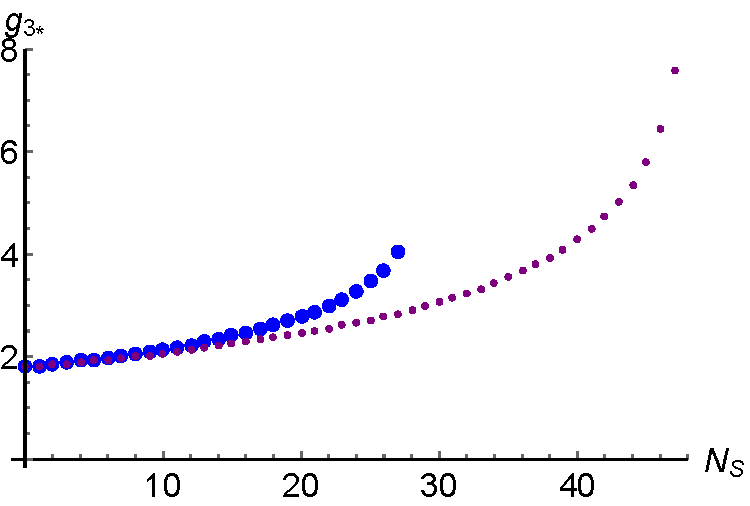
\includegraphics[width=\linewidth]{g3_Ns_no_etas.pdf}\\
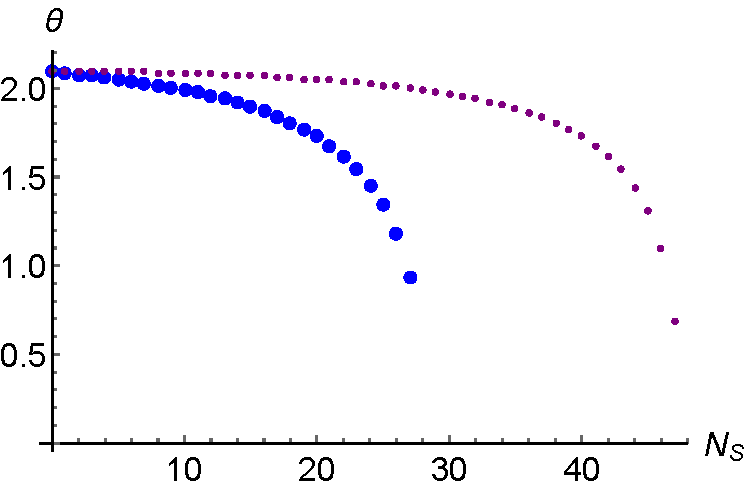
\includegraphics[width=\linewidth]{theta_Ns_no_etas.pdf}
\caption{\label{g3Nsnoetas}We show the fixed point value for $g_3$ (upper panel)
and the critical exponent $\theta$ (lower panel) as a function of $N_S$.
The larger blue dots denote the full result and the smaller purple dots the semi-perturbative approximation.}
\end{figure}

\begin{figure}
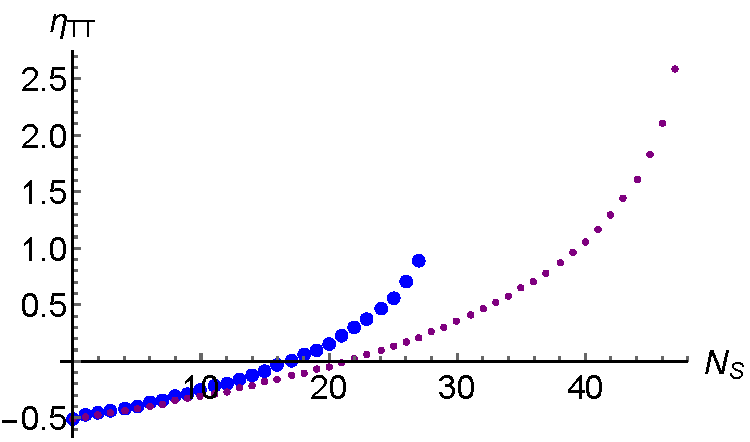
\includegraphics[width=0.45\linewidth]{etaTT_Ns_no_etas.pdf}\quad
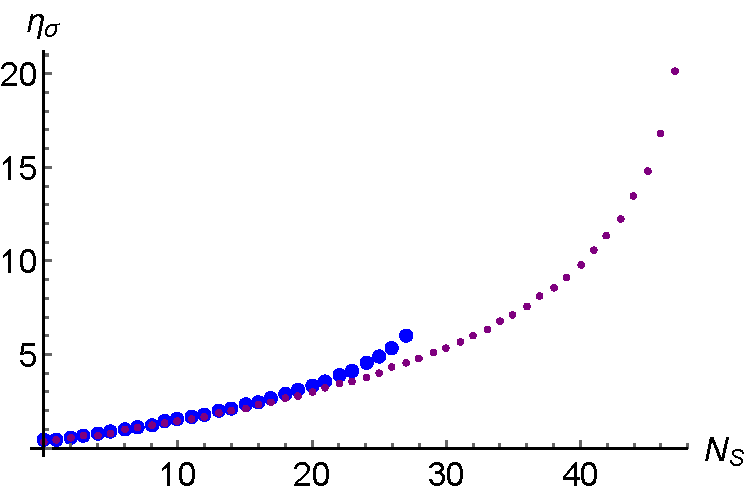
\includegraphics[width=0.45\linewidth]{etasigma_Ns_no_etas.pdf}
\caption{\label{etaNsnoetas}We show the fixed point value for $\eta_{\rm TT}$ (left panel)
and $\eta_{\sigma}$ (right panel) as a function of $N_S$.
The larger blue dots denote the full result and the smaller purple dots the semi-perturbative approximation.}
\end{figure}



\begin{figure}
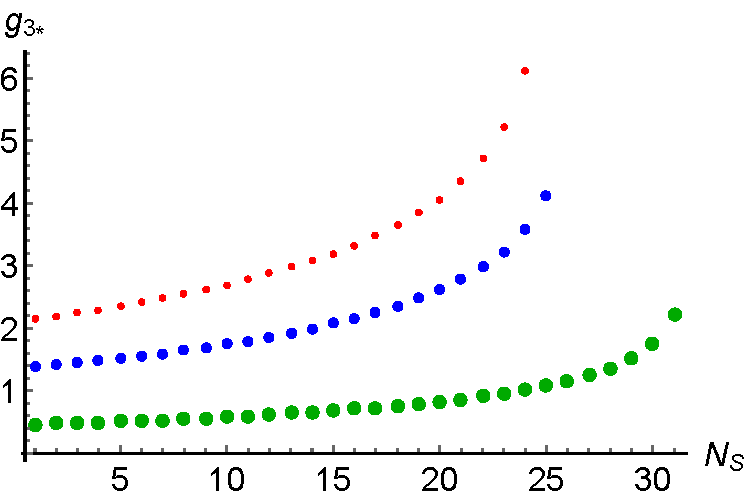
\includegraphics[width=\linewidth]{g3_Ns_G3.pdf}\\
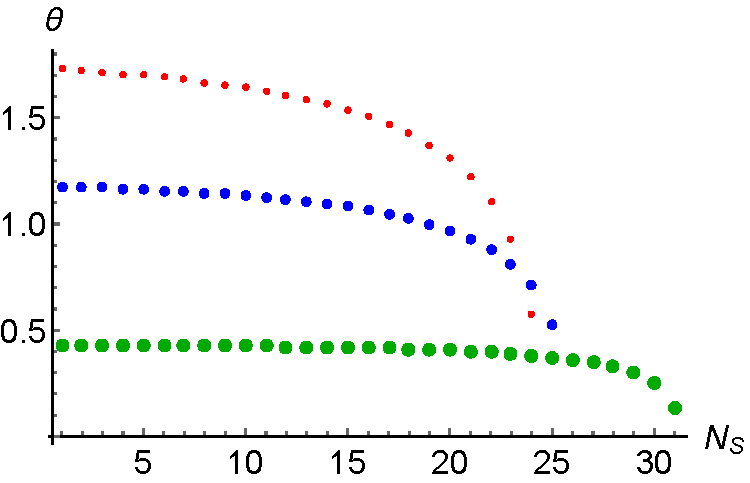
\includegraphics[width=\linewidth]{theta_NS_G3.pdf}
\caption{\label{g3NsnoetasG3}We show the fixed point value for $g_3$ (upper panel)
and the critical exponent $\theta$ (lower panel) as a function of $N_S$.
The small red dots are for $G_3=G_4=1$,
the medium blue ones for $G_3=G_4=3$ and the large green ones for $G_3=G_4=6$.}
\end{figure}

\begin{figure}
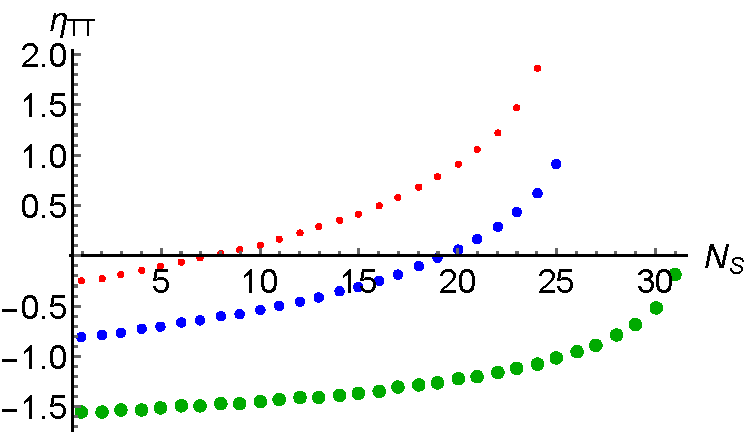
\includegraphics[width=0.45\linewidth]{etaTT_NS_G3.pdf}\quad
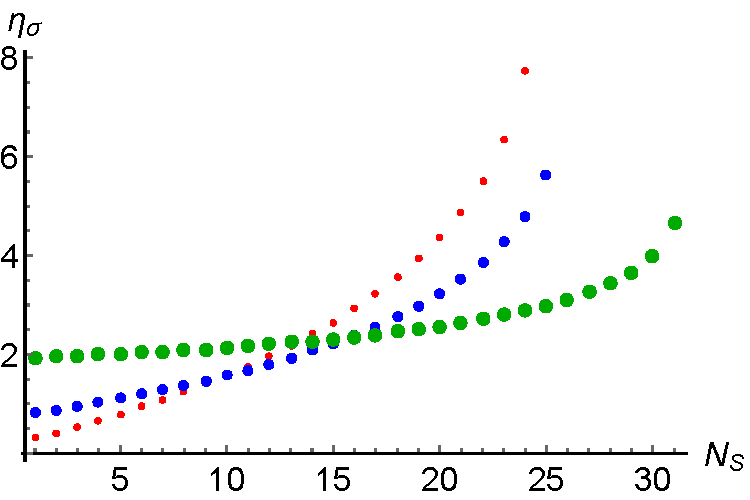
\includegraphics[width=0.45\linewidth]{etasigma_NS_G3.pdf}
\caption{\label{etaNsnoetasG3}We show the fixed point value for $\eta_{\rm TT}$ (left panel)
and for $\eta_{\sigma}$ (right panel) as a function of $N_S$.
The small red dots are for $G_3=G_4=1$, the medium blue ones for $G_3=G_4=3$ and the large
green ones for $G_3=G_4=6$.}
\end{figure}


To investigate the stability of our results,
we again distinguish the pure-gravity couplings from the gravity-matter couplings.
We treat $G_4=G_3$ as an external parameter,
and investigate the fixed point in $g_3$ as a function of $G_3$ and $N_S$.
In particular, at smaller $G_3$, the value of $\eta_{\sigma}$ at small $N_S$ remains smaller.
We observe that larger values of $G_3$ lead to a slower increase in the fixed-point value for $g_3$,
and increase the value $N_S$ at which the fixed-point annihilation occurs,
cf.~Fig.~\ref{g3NsnoetasG3}.
While quantitative details change, the overall effect of increasing $N_S$ is similar to
the previous approximation, cf.~Fig.~\ref{etaNsnoetasG3}.
This suggests that our results will be qualitatively stable under extensions of the truncation
including the running of the gravity-couplings as in \cite{Meibohm:2015twa}.
On the other hand, a non-trivial interplay between the gravity-matter coupling
and the pure-gravity coupling at large $N_S$ is not excluded,
as the effect of varying $g_3$ on $G_{3\, \ast}$  remains to be studied.


\subsection{Fixed-point results including scalar anomalous dimension}
\label{FPwithmatterincludingetas}

We now set all gravitational couplings and gravity-scalar couplings equal to the Newton
coupling as defined from the gravity-matter interaction and include the anomalous dimension for the scalar,
$\eta_S$. This yields a new contribution to $\beta_{g_3}$, which now reads
\be
\beta_{g_3}=2 g_3 + 2 g_3 \eta_S-
\frac{1}{6\pi}g_3^2\left(20-\frac{N_S}{4}+\frac{23}{60}\eta_S\right)
+\mathcal{O}(g_3^3).
\ee
Using
\be
\eta_S = \frac{7}{4 \pi}g_3 + \mathcal{O}(g_3^2)
\ee
equation (\ref{norma}) gets replaced by
\be
\beta_{g_3}= 2g_3+\frac{4+N_S}{24\pi}g_3^2
+\mathcal{O}(g_3^3).
\ee
Therefore, in this simplified form,
the terms of order $g_3^2$ in the beta function
are always positive, and by themselves would
not produce a fixed point.
Fixed points appear when we consider also higher nonlinearities,
but their properties are not very stable.

For small numbers of scalars, both in the semi-perturbative
approximation and using the full equations, we have,
in addition to the Gaussian fixed point,
also two non-trivial fixed points.
The first, which we call $FP_1$, has
negative $g_3$ and the second, which we call $FP_2$,
has positive $g_3$.
The fixed point $FP_1$ cannot be immediately
discarded on the basis of having a negative $g_3$.
While a negative value of the Newton coupling in the infrared is of course incompatible with observations,
a negative fixed-point value is viable, as long as the RG flow can cross to $g_3>0$ towards the IR.
As the full beta function contains terms $\sim g_5$ etc., which imply $\beta_{g_3}\neq0$ at $g_3=0$,
this situation is realized here.

In the semi-perturbative approximation the solutions
of the fixed point equation can be written explicitly:
\be
g_{3*}=\frac{9\pi\left(60+15N_S\pm\sqrt{41904-2008N_S+45N_S^2}\right)}{1287-74N_S}
\ .
\ee
The solution $FP_2$ (which corresponds to the positive sign
in front of the root) is a growing function of $N_S$, with a simple pole
between $N_S=17$ and $18$ and asymptotes to $-135\pi/37$
for large $N_S$.
The solution $FP_1$ is a negative, smooth, monotonically increasing function
of $N_S$ that asymptotes to zero.

The solutions of the full equations are more complicated to display
in closed form and are best studied numerically.
Let us start from the case $N_S=1$.
The properties of the fixed points in the two approximations
are listed in~tab.~\ref{FPtab3}.

\begin{table}[]
  \begin{center}
    \begin{tabular}{ l r r r r r }
      \toprule
      approximation            & $g_{3\,\ast}$ & $\theta$ & $\eta_{\rm TT}$ & $\eta_{\sigma}$ & $\eta_S$ \\
      \midrule
      $FP_1$ full              & -13.9         & 3.85     & 3.27            & -0.31           & -6.50 \\
      $FP_1$ semi-perturbative & -8.67         & 3.42     & 2.34            & -1.92           & -4.83 \\
      $FP_2$ full              & 53.4          & 11.7     & -5.21           & 10.8            & 25.2  \\
      $FP_2$ semi-perturbative & 12.2          & 4.81     & -3.28           & 2.69            & 6.78  \\
      \bottomrule
    \end{tabular}
  \end{center}
  \caption{
    Coordinates and critical exponents of the interacting fixed points at $N_S=1$,
    both in semi-perturbative and full approximations.
  }
  \label{FPtab3}
\end{table}


The properties of the fixed points in the two approximations
are very roughly consistent, but $FP_2$ in the full approximation
has very large critical exponent and anomalous dimensions,
that put it far beyond the regime where our approximation is reliable.


The similarities end here, because the dependence on $N_S$
is quite different in the two approximations.
In the full calculation, $g_{3*}$ for $FP_2$,
as a function of $N_S$, is initially decreasing,
has a minimum near $N_S=30$,
then increases again and the fixed point
ceases to exist for $N_S>95$.
It switches from UV attractive to repulsive near $N_S=47$
and there is no value of $N_S$ for which the critical exponents
have reasonably small values.
This is very different from its behavior in the semi-perturbative
approximation.

Also $FP_1$ in the full calculation behaves very differently from
the semi-perturbative approximation:
instead of increasing steadily to zero, it decreases monotonically
and diverges to $-\infty$ for $N_S$ just above $46$.
Some of the anomalous dimensions have more reasonable values
but there is no $N_S$ for which they are all small.
Thus $FP_1$ has slightly better chances of being
a true fixed point, but in the present approximations
it cannot be reliably assessed.



\begin{figure}
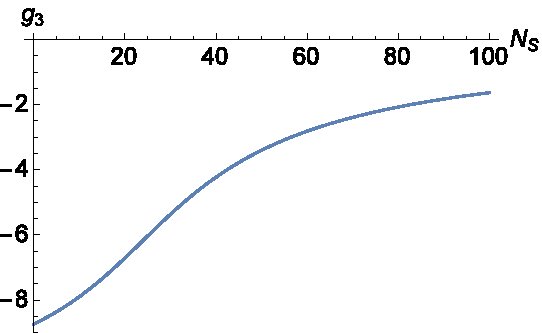
\includegraphics[width=0.45\linewidth]{g3_Ns_equalcouplings.pdf} \quad 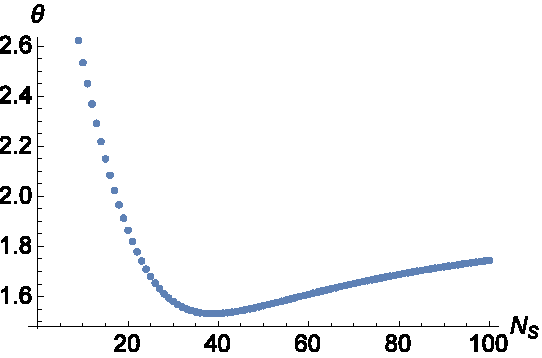
\includegraphics[width=0.45\linewidth]{theta_Ns_equalcouplings.pdf}\newline
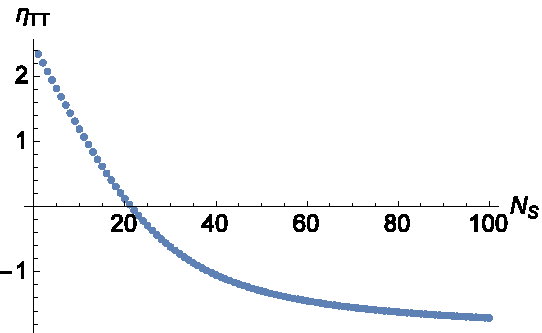
\includegraphics[width=0.45\linewidth]{etah_Ns_equalcouplings.pdf} \quad 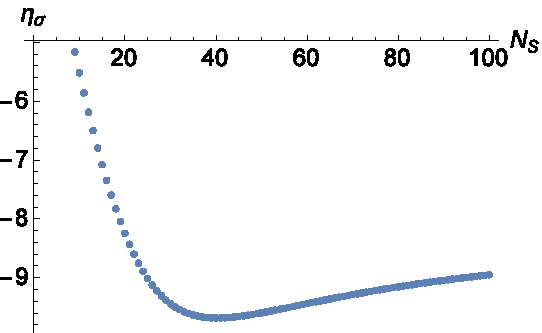
\includegraphics[width=0.45\linewidth]{etasigma_Ns_equalcouplings.pdf}\newline
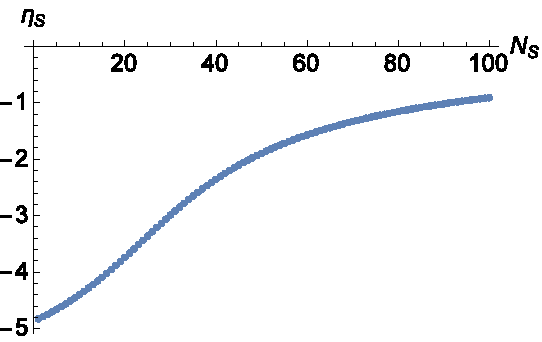
\includegraphics[width=0.45\linewidth]{etas_Ns_equalcouplings.pdf}
\caption{\label{FPNsequalcouplings} We show results in the semi-perturbative approximation:
We plot the fixed-point value for $g_3$ as a function of $N_S$ (left upper panel)
and the value of the critical exponent $\theta$ (right upper panel), as well as the anomalous dimensions.}
\end{figure}


We observe that already in the case $N_S=1$
the anomalous dimensions of the graviton modes
have opposite signs compared to the case when we neglected $\eta_S$,
and become rather large, as a consequence of a rather large absolute value of $g_3$.
The critical exponent also differs considerably from the pure-gravity case.
As a consequence, when we take into account the effect of
$\eta_S$, it becomes hard to identify either of the fixed points
with the one that we found for $N_S=0$.

These results could lead to different conclusions:
the approximation $G=g$ might not be particularly reliable
beyond small $N_S$, or, more likely, our current estimate
for the scalar anomalous dimension needs improvement,
and the results for $\eta_S=0$ might be closer to the correct result.

The significant change in the fixed-point properties from the pure-gravity case arises from
the scalar anomalous dimension.
Accordingly, the perturbative approximation, where $\eta_{TT}=\eta_{\sigma}=\eta_S=0$
features a fixed point at $g_3=2.57$ with $\theta=2$
for all values of $N_S$.
As $\eta_S$ has such a significant effect on the existence and properties of fixed points,
it is important to understand
whether our truncation already captures all major operators
that determine $\eta_S$. Recall that metric fluctuations
induce non-vanishing momentum-dependent
matter self-interactions, e.g., of the form $\left(g^{\mu \nu} \partial_{\mu} \phi \partial_{\nu}\phi\right)^2$ \cite{Eichhorn:2012va}. As soon as these couplings
are non-zero, they yield a nonvanishing contribution to $\eta_S$.
Our current truncation does not include these effects.
We therefore conjecture that the results could improve
once these further operators are included.
By a simple count of modes, $N_S=1$ should not
dramatically change the results, and the case $N_S=1$
should still feature a fixed point
with properties similar to the pure-gravity one,
just as exhibited by the approximation $\eta_S=0$.
We tentatively suggest that the calculation with $\eta_S=0$,
which shows a destablizing effect setting in at $N_S\gg1$,
might capture the full dynamics more accurately than our current estimate with $\eta_S \neq 0$.



\subsection{Background beta functions}
%
The background couplings can only appear on the right-hand side of beta functions through a trivial scaling,
for instance, $\beta_{\bar{G}} \sim \bar{G}^2$,
as the prefactor of the curvature term in the Einstein-Hilbert action is $\frac{1}{16 \pi \bar{G}}$.
All couplings that appear on the right-hand side from either propagators or vertices are always
fluctuation field couplings.
Accordingly, $\eta_{\rm TT}$, $\eta_{\sigma}$ and $\eta_S$,
which will appear on the right-hand side of $\beta_{\bar{G}}$,
depend on the fluctuation-field couplings $g_3$, $g_4$, $g_5$, $G_3$, $G_4$ only.
Thus we obtain the following matter contribution to the $\beta$ function for the background Newton coupling:
\be
\beta_{\bar{G}}\Big|_{\rm scalar}=\frac{\bar{G}^2}{24 \pi}N_S (4-\eta_S).
\ee

Following \cite{Percacci:2015wwa},
\bea
\beta_{\bar{G}}=2 \bar{G}
- \frac{\bar{G}^2}{\pi} \left(\frac{15}{8}
- \frac{5 \eta_{\rm TT}}{18 }
+ \frac{\eta_{\sigma}}{24}
-  \frac{N_S}{24} (4 - \eta_{S})\right).
\eea

If we set $\eta_{\rm TT}= \eta_{\sigma}=0=\eta_S$, we obtain $N_S=45$ as the maximal
number of scalars before the fixed point in $\bar{G}$ diverges.

If we now use the approximation of equating all fluctuation couplings in the expressions
for the anomalous dimensions, as in Sec.~\ref{FPwithmatterincludingetas},
we obtain a fixed point at $\bar{G}_{\ast}=12.14$, with critical exponent $\theta=2$,
for $N_S=1$  at the fixed point $g_{\ast}=-13.9$.
 The location of a possible bound depends on the assumptions for the couplings $g_4, g_5$, $G_3, G_4$.
 For the case $g_4=0=g_5$, $G_3=0=G_4$,
 the continuation of the pure-gravity fixed point in the background coupling ceases to exist beyond $N_S=9$.

For the approximation where we set $\eta_S=0$, we obtain a bound at $N_S=12$,
which is close to the bound from the fluctuation coupling, at $N_S=14$.

Note that fixed-point values for the background couplings are affected by a strong regulator dependence:
As the background metric enters the regulator function,
there are contributions to all beta functions of background couplings that are due to the regularization only,
and are unphysical in that sense, see also \cite{Folkerts:2011jz, Litim:2002ce, Litim:2002hj, Bridle:2013sra}.
Thus, even divergences in background couplings might turn out to be compatible with a model that
is asymptotically safe in a physical sense, i.e., where all physical quantities have a well-behaved UV limit.
To understand on which couplings a fixed-point requirement must be imposed,
and which couplings may even diverge, one must investigate physical observables.
As this is clearly beyond the scope of the present work, we conclude that the most conservative
assumption is that \emph{all} couplings must feature fixed points,
and therefore divergences in the background couplings are not acceptable,
even if the fluctuation couplings are well-behaved. Interpreted along these lines,
the one-loop approximation, where we set $\eta_{\rm TT}=\eta_{\sigma}=0=\eta_S$ everywhere,
and only the background Newton coupling depends on $N_S$,
would suggest that there could be an upper limit of scalars that is compatible with a viable fixed point.
\newline\\

%
\section{Conclusions}
%
In this work, we discuss how setting up a Renormalization Group flow for gravity-matter systems,
in order to investigate the viability of the asymptotic safety scenario for gravity and the Standard Model,
necessitates a distinction between couplings of matter to the background metric and couplings to
fluctuations of the metric.
We take a first step in disentangling the scale-dependence of the different couplings by studying
the running of a vertex at which two scalar fields interact with the metric fluctuation field.
From this vertex we define an avatar of the Newton coupling, $g_3$.
We observe that the so-defined Newton coupling features an interacting fixed point at $N_S=0$
where only metric fluctuations drive the Renormalization Group flow.
The universal critical exponent at this fixed point is close to that of other approximations and definitions.
We consider this rather strong evidence for the asymptotic safety scenario  in the pure-gravity case,
that complements previous results.
We emphasize that this is the first evidence for asymptotic-safety in gravity-matter interactions,
as all previous results related to the Newton coupling defined from background or fluctuation
gravitational interactions.
Our result is therefore a new hint that formulating an asymptotically safe theory of gravity
and matter could be phenomenologically viable.\newline

We also investigate the anomalous dimensions for different components of the graviton,
and find a large negative anomalous dimension $\eta_{\rm TT}$ for the TT mode,
which is not too far from the single-metric approximation $\eta_N=-2$.
Such a large negative anomalous dimension implies a strongly UV suppressed propagator of the form
$p^{-2+\eta_{TT}}$. The corresponding propagator in real space is reminiscent of a lower-dimensional setting.
Thus our result is in line with other indications for some form of dynamical dimensional reduction
in asymptotically safe gravity
\cite{Lauscher:2001ya, Lauscher:2005qz, Reuter:2011ah, Rechenberger:2012pm, Calcagni:2013vsa},
however see also \cite{DOdorico:2015jtl}.

On the other hand, the  $\sigma$-anomalous dimension has the opposite sign.
This suggests that different tensor structures in gravity exhibit different running---reminiscent
of the difference between the transverse and longitudinal gluons in the infrared regime
in Yang-Mills theory in Landau gauge.
This result is an indication that one should also disentangle the flow of different tensor structures
at the level of the vertices.
We moreover observe a difference to results in the linear parametrization,
where the anomalous dimensions are typically smaller in  absolute value.

Within functional Renormalization Group flows, it is never possible to find a finite-dimensional
closed truncation, as higher-order couplings always couple back into the flow of lower-order ones.
For instance, the flow of the coupling $g_3$ depends on the higher-order coupling $g_5$ through
a tadpole diagram. Thus, one should evaluate the flow for $g_5$,
which itself depends on $g_7$ and so on, necessitating some approximation to close the truncation.
Typical choices in the literature include setting higher-order couplings to zero,
or equating them to lower order ones. In our results,
we explicitly keep the dependence on all couplings that enter $\beta_{g_3}$,
enabling us to study the reliability of different approximations:
We observe that the choice of approximation for those couplings for which no beta function is
determined explicitly, quantitatively alters the properties of the fixed point: By treating,
e.g., the pure-gravity couplings $G_3$ and $G_4$ as external parameters, we observe that the
fixed point in $g_3$ persists for all values of these couplings that we have investigated,
but, e.g., anomalous dimensions and the critical exponent change.
It is reassuring that the existence of a fixed point does not  depend on making specific choices
for couplings for which no beta function is determined, as of course all results in the literature
make specific choices for these couplings. On the other hand,
our investigation of the dependence of fixed-point properties on these choices highlights that quantitatively
more precise results require
 more elaborate truncation schemes which disentangle some of these couplings.


In the case $N_S>0$, scalar fluctuations have a significant impact.
If we work in the approximation where we set the anomalous dimension for the scalar matter field to zero,
$\eta_S=0$, we observe that matter fluctuations  have a destabilizing effect on the gravitational fixed point,
and move it toward larger values.
This observation is in accordance with the general scenario discussed at the level of the
background couplings in \cite{Dona:2013qba, Dona:2014pla},
where it is argued that the inclusion of dynamical matter degrees of freedom will impact
the microscopic dynamics for gravity, and an increasing number of scalars leads to a growth of the
fixed point value for the Newton coupling. In \cite{Meibohm:2015twa} a similar behavior
is found for the fluctuation coupling $G_3$.
The increasing fixed-point value leads to an increase in the anomalous dimension for the graviton.
As our regularization scheme requires $\eta<2$ for all anomalous dimensions,
the region of $N_S \geq 14$ requires a re-investigation with a different regularization
scheme and/or significantly larger truncations.
We should therefore take care when interpreting our present results.
Keeping in mind this word of caution, we observe that scalar matter seems to have a significant
effect on an interacting fixed point and could potentially destabilize it.
On the other hand, it is reassuring to observe that $N_S=4$,
which is of course the phenomenologically most relevant case as it corresponds to the number of
scalar fields in the Standard Model,
admits a gravitational fixed point in our setting,
again in line with results in \cite{Dona:2013qba, Dona:2014pla, Meibohm:2015twa}.

Including a scalar anomalous dimension $\eta_S$ leads to a very significant change
of the fixed-point properties already at $N_S=1$.
Based on a mode-counting argument, we
expect that this strong effect of a single scalar field only arises within our truncation,
and such significant effects of matter should not be expected for small $N_S$.
We also identify a direction in which an extension of our truncation would potentially
lead to $\mathcal{O}(1)$ changes of the anomalous dimension for scalars:
Quantum-gravity effects induce non-vanishing momentum-dependent self-interactions
for scalars \cite{Eichhorn:2012va}, which will couple into $\eta_S$ via a tadpole diagram.
If we take into account quantum-gravity induced matter self-interactions, not only $\eta_S$ will change.
Among the diagrams contributing to $\beta_{g_3}$,
there will also be one that features a closed scalar loop,
and thus yields a contribution that scales with $N_S$. Within our present approximation,
there is no such explicit contribution, and the $N_S$ dependence only arises through the anomalous dimensions.

Moreover, it will be interesting to understand the parametrization and gauge-dependence of our result.
As the matter-gravity vertices differ signficiantly between,
e.g., Landau gauge and linear parametrization on the one hand,
and unimodular gauge and exponential parametrization on the other hand,
the structure of the beta function for $g_3$ as well as $G_3$ could be significantly different.
Thus, it will be interesting to understand whether the observations in the present work as
well as in \cite{Meibohm:2015twa} persist,
if the system $\beta_{g_3}, \beta_{G_3}$ is analyzed in the two different parametrizations.
In particular, it will be interesting to see whether the sign of the contribution
$\sim N_S$ to $\beta_{g_3}$ and $\beta_{G_3}$ depends on the choice of parametrization.


%----------------------------------------------------------------------------------------
% CHAPTER 3
%----------------------------------------------------------------------------------------

\chapter{Background Independence}


\section{Introduction}
\label{sec:introduction}

Following ref. \cite{Reuter:1996cp},
non-perturbative RG (renormalization group) flows for quantum gravity have been formulated
by utilising the technical device of splitting the metric in terms of a background metric
and a fluctuation field (see also the reviews
\cite{Reuter:2012id, Percacci:2011fr, Niedermaier:2006wt, Nagy:2012ef, Litim:2011cp}).
Physical results must then be independent of this split, in other words should be background independent.
The background metric however is in particular also used (via the background Laplacian)
to define the effective cutoff scale $k$.
This breaks background independence at intermediate scales $k$ but such that background
independence can be recovered in the limit $k\to0$ providing certain modified split Ward
identities (msWIs) are imposed
\cite{Pawlowski:2005xe, Litim:2002hj, Bridle:2013sra, Reuter:1997gx, Litim:1998nf, Litim:2002ce,
Manrique:2009uh, Manrique:2010mq, Manrique:2010am, Dietz:2015owa, Safari:2015dva}.



An unsettling conclusion from the research reported in ref. \cite{Dietz:2015owa} is that the requirement of background independence in a theory of quantum gravity can actually be in conflict with renormalization group (RG) properties in flows formulated as above: fixed points under changes in the effective cutoff scale $k$, can be forbidden by the msWIs  that are enforcing background independence.\footnote{Very recently an alternative approach has been initiated which avoids these issues entirely since background independence is never broken \cite{Morris:2016nda}.}

In the conformally truncated gravity model investigated in ref.  \cite{Dietz:2015owa}, this happens generically when the anomalous dimension $\eta$ is non-vanishing.
It can however be avoided by a careful choice of parametrisation $f$ (setting it to be a power of $\chi$ determined by its scaling dimension \cite{Dietz:2015owa}).
On the other hand it was shown in ref. \cite{Dietz:2015owa} that the situation is saved in all cases, at least in the conformally reduced gravity model, by the existence of an alternative background-independent description. This involves in particular a background-independent notion of scale, $\hat{k}$. This background independent description exists at a deeper underlying level since in terms of these background-independent variables, the RG fixed points and corresponding flows always exist, and are manifestly independent of the choice of parametrisation $f(\chi)$.

After approximating the exact RG flow equations and msWIs to second order in the derivative expansion (as will be reviewed later),
%(for $\varphi$, the fluctuation part of the conformal factor)
the crucial technical insight was to notice that, just as in the scalar field theory model
\cite{Bridle:2013sra}, the msWIs and RG flow equations can be combined into linear partial differential equations. It is the solution of the latter equations by the method of characteristics, that uncovers the background independent variables. And it is by comparing the description in these variables with the equivalent description in the original variables,
that we see that fixed points in the original variables are in general forbidden by  background independence.

However in order to facilitate combining the RG flow equations and msWIs when the anomalous dimension $\eta\ne0$, the authors of ref. \cite{Dietz:2015owa} were led to a particular form of cutoff profile $R_k$, namely a power-law cutoff profile. We will show in this paper that in fact this cutoff profile plays a r\^ole that is much deeper than the convenience of this mathematical trick.
%If $\eta\ne0$, we \emph{must} use this cutoff profile in the derivative expansion approximation.
%,  as can be seen by considering a question that was overlooked in ref. \cite{Dietz:2015owa}.
Whilst at the exact level the msWIs are guaranteed to be compatible with the exact RG flow equation (for completeness and later purposes we provide a proof in sec. \ref{sec:exact}), this will typically not be the case once approximated.
%As we will see, even in an otherwise unrestricted derivative expansion, compatibility requires extra conditions.
We will see that in the $O(\partial^2)$ derivative expansion approximation derived in ref. \cite{Dietz:2015owa}, the msWI and flow equations are in fact compatible {if and only if} either the cutoff profile is power law, or we have the special case that $\eta=0$.


If the msWIs are not compatible with the flow equations, it does not immediately follow that there are no simultaneous solution to the system of equations. However, as we argue in sec. \ref{sec:incompatibility} and verify by example in sec. \ref{sec:incompatible-no-solns} (see also sec. \ref{sec:truncations}), if the msWIs are not compatible, the equations are overconstrained and it is for this reason that it is hopeless to expect any solutions.

The example is furnished by choosing optimised cutoff profile and LPA, but keeping $\eta$ non-vanishing.
In fact it is natural to expect $\eta$ to be non-vanishing at the LPA level for conformally truncated gravity, as explained in ref. \cite{Dietz:2016gzg}.  Choosing a power-law form for $f$ the equations at first sight then look consistent and able to support fixed points. Although we already know that the msWI is in this case incompatible with the flow equation, it is still possible to combine the msWI and flow equation into a linear partial differential equation. Solving this, we confirm that for the combined system there are no solutions with $\eta\ne0$, supporting the arguments in sec. \ref{sec:incompatibility}. In sec. \ref{sec:truncations}, by considering the simplest polynomial truncation, we also verify very straightforwardly that there can be no fixed points.

For power-law cutoff profile the equations are compatible, however we will see very clearly in sec. \ref{sec:forbids} why with $\eta\ne0$ and non-power-law parametrisation $f$, there can be no fixed points with respect to $k$.

Actually, power law cutoff profiles have nice properties in  that they ensure that the derivative expansion approximation preserves the quantisation of the anomalous dimension in non-gravitational systems,
\eg scalar field theory
\cite{Morris:1994ie, Morris:1994jc, Morris:1998da}.%
\footnote{Although as with the optimised cutoff \cite{Litim:2000ci, Litim:2001fd},
they do not allow a derivative expansion to all orders \cite{Morris:2005ck, Morris:1999ba, Morris:2000hm}.
}
Nevertheless, given the unsettling nature of the conclusions in ref.
\cite{Dietz:2015owa}, it is important to understand  to what extent the results depend on cutoff profile.

Since $\eta=0$ is sufficient to allow the derivative expansions of the exact RG and msWI equations to be compatible, we can therefore investigate in this case the implications of background independence, whatever the cutoff profile. The conclusions are the same for any cutoff profile that is not power law, so for simplicity and to make the equations completely explicit, we take the popular and simple choice of optimised cutoff \cite{Litim:2000ci, Litim:2001fd}.  Just as found for power law cutoff \cite{Dietz:2016gzg} in this case, background-independent variables exist, and $k$-fixed points exist; these coincide with the fixed points in background-independent variables.  In terms of background-independent variables and at LPA level, the full line of fixed points
is visible, confirming the findings for power-law cutoff \cite{Dietz:2016gzg}.


Although we can show this by exact analysis of the LPA flow and msWI equations, using the trick of combining these equations into a linear partial differential equation, it is very instructive to analyse these equations without using this trick and also by considering only polynomial truncations, since it seems likely that this is the only way we could investigate this issue using the exact non-perturbative flow equations. Viewed from this perspective, we will see that the problem is that if the RG fixed point equations and msWI equations are truly independent, then they will overconstrain the solutions if carried to sufficiently high order truncation. Indeed, expanding in powers of the fluctuation field $\vp$ to the $m^{\rm th}$ level and background field $\chi$ to the $n^{\rm th}$ level, we get one fixed point equation for each $(m,n)$-point vertex \emph{and} one msWI equation per vertex. Even though each of these equations is open (depending on yet higher-point vertices) we will see that since there are two equations for every vertex, at sufficiently high order truncation there are more equations than vertices (indeed eventually double the number) and thus either the equations become highly redundant or the vertices are constrained to the point where there are no solutions.



This analysis strongly suggests therefore that the full non-perturbative Ward identities would lead to important constraints on RG properties. Unfortunately it seems very challenging to investigate this, since we will see that the number of equations only exceeds the number of vertices for the first time  at the six-point level.
We discuss potential conflict for the exact non-perturbative flow equations further in the conclusions.



\section{Conformally reduced gravity at order derivative-squared}\label{sec:review}

In this section we give a quick resum\'e of the results we need and their context, from ref. \cite{Dietz:2015owa}.
%
%Background field method
%\begin{equation}
%	g_{\mu\nu} =   \bar g_{\mu\nu} + \tilde g_{\mu\nu} \,.
%\end{equation}
%Conformally reduced gravity setting \cite{Dietz:2015owa}:
We arrive at conformally reduced gravity (in Euclidean signature) by writing:
\begin{equation}
\label{conformal-reduction}
	\tilde g_{\mu\nu} = f(\tilde\phi) \hat g_{\mu\nu}= f(\chi +\tilde\varphi )\hat g_{\mu\nu} \qquad\text{and} \qquad \bar g_{\mu\nu} = f(\chi)\hat g_{\mu\nu} \,.
\end{equation}
Here $\tilde g_{\mu\nu}$ is the metric that is integrated over in the partition function. It is restricted to an overall conformal factor $f(\tilde\phi)$ times a fiducial metric which in fact we set to flat: $\hat g_{\mu\nu}=\delta_{\mu\nu}$.

Examples of parametrisations used previously in the literature include
$f(\phi) = \exp(2\phi)$ \cite{Machado:2009ph} and $f(\phi)=\phi^2$ \cite{Manrique:2009uh,Bonanno:2012dg}. However we leave the choice of parametrisation $f$ unspecified. It is important to note however that $f$ cannot depend on $k$ since it is introduced at the bare level and has no relation to the infrared cutoff (moreover if $f$ depended on $k$, the flow equation \eqref{equ:flowGamma} would no longer hold).  Later we will change to dimensionless variables using $k$ and in these variables it can be forced to depend on $k$   (see especially secs. \ref{sec:required-cutoff} and \ref{sec:forbids}).

We split the total conformal factor field $\tilde\phi(x)$ into a background conformal factor field $\chi(x)$ and fluctuation conformal factor field $\tilde\vp(x)$. It is then the latter that is integrated over. Also as shown, we similarly parametrise the background metric $\bar{g}_{\mu\nu}$ in terms of the background conformal factor field $\chi$. Introducing the classical fluctuation field $\vp = \langle \tilde \vp \rangle$ and total classical field $\phi = \langle \tilde \phi \rangle = \chi + \vp$, the effective action  satisfies the flow equation
\be
\label{equ:flowGamma}
\partial_t \Gamma_k[\vp,\chi] = \frac{1}{2}\mathrm{Tr}\left[\frac{1}{\sqrt{\bar g}\sqrt{\bar g}}\frac{\delta^2\Gamma_k}
				  {\delta \vp \delta \vp}+ R_k[\chi]\right]^{-1} \partial_t R_k[\chi]\,.
\ee
 Here we have introduced the RG time
\be
\label{time}
t=\ln(k/\mu)\,,
\ee
with $\mu$ being a fixed reference scale, which can be thought of as being the usual arbitrary
finite physical mass-scale.
$R_k$ is the cutoff operator responsible for suppressing momentum modes below the
infrared cutoff scale $k$, \cf \cite{Wetterich:1992yh, Morris:1993qb}.
The crucial observation is that in the context of the background field method in quantum gravity the cutoff operator itself depends on the background field $\chi$. The reason for this is that the cutoff operator is a function of the covariant Laplacian of the background metric $R_k\left(-\bar \nabla^2\right)$, as it is with respect to the spectrum of $-\bar\nabla^2$ that modes are integrated out or suppressed in the path integral, \cf \cite{Reuter:2008wj,Reuter:2009kq}.

A remnant diffeomorphism invariance enforces this $\chi$ dependence in the approximation chosen in ref. \cite{Dietz:2015owa}.
By specialising to a background metric ${\bar g}_{\mu\nu}$ that is slowly varying, so that space-time derivatives of this can be neglected, we
effectively terminate at the level of the LPA for the background conformal factor $\chi$. For the classical fluctuating conformal factor $\vp$ however,  $\mathcal{O}(\partial^2)$ in the derivative expansion approximation is fully implemented, making no other approximation.
The effective action thus takes its most general form at this level of truncation:
\begin{equation}
\label{trunc}
	\Gamma_k[\varphi, \chi] = \int d^dx \sqrt{\bar g} \left( -\frac{1}{2}K(\varphi,\chi)
	\bar g^{\mu\nu}\partial_{\mu}\varphi\partial_{\nu}\varphi + V(\varphi,\chi)  \right)\,.
\end{equation}
The msWI encodes the extent to which the effective action violates split symmetry:
\be
\label{equ:split-symmetry}
\tilde \vp(x) \mapsto \tilde \vp(x) + \eps(x) \qquad \chi(x) \mapsto \chi(x) -\eps(x)\,.
\ee
Due to the special r\^ole played by $\chi$, the infrared cutoff operator breaks this symmetry, leading to the msWI:
\be
\label{equ:sWiGamma}
\frac{1}{\sqrt{\bar g}}\left(\frac{\delta\Gamma_k}{\delta \chi}-\frac{\delta \Gamma_k}{\delta \vp}\right)
      =\frac{1}{2}\mathrm{Tr}\left[\frac{1}{\sqrt{\bar g}\sqrt{\bar g}}\frac{\delta^2\Gamma_k}
				  {\delta \vp \delta \vp}+ R_k[\chi]\right]^{-1} \frac{1}{\sqrt{\bar g}}
				  \left\{\frac{\delta R_k[\chi] }{\delta \chi}+\frac{d}{2}\dclnf R_k[\chi]\right\}\,.
\ee
Exact background independence would be realised if the right hand side of the msWI was zero, implying that the effective action is only a functional of the total field $\phi = \chi + \vp$. The presence of the cutoff operator however causes the right hand side to be non-vanishing in general. It is only in the limit $k\rightarrow0$ (holding physical, \ie unscaled, momenta and fields fixed) that the cutoff operator drops out and background independence can be restored exactly. We note therefore that imposing the msWI in addition to the flow equation \eqref{equ:flowGamma} automatically ensures exact background independence in the limit $k\rightarrow0$. The observation we further explore in this paper is that restricting flows to satisfy \eqref{equ:sWiGamma} then has consequences for the RG properties, in particular fixed point behaviour, that follows from \eqref{equ:flowGamma}.



%\footnote{The source term also breaks split invariance but does not contribute to the separate background field dependence in $\Gamma_k[\vp,\chi]$, as the ensuing calculation shows.}  \cf \cite{Becker:2014qya,Reuter:2008qx,Bridle:2013sra}. It is the violation of split symmetry that signals the loss of background independence, both at the level of the functional integral and at the level of the effective action.

Computing the flow equation and msWI in the derivative expansion \eqref{trunc} results in flow equations and modified split Ward identities\footnote{Although we always mean these modified identities, we will sometimes refer to them  simply as Ward identities.},  for the potential $V$:
\begin{align}
	\label{flowV}
	\partial_t V(\varphi,\chi) &= f(\chi)^{-\frac{d}{2}}\int dp\, p^{d-1} Q_p\dot R_p \,,\\
	\label{msWIV}
	\partial_\chi V - \partial_\varphi V +\frac{d}{2}\partial_\chi \text{ln} f V
	&= f(\chi)^{-\frac{d}{2}}\int dp\, p^{d-1} Q_p\left(\partial_\chi R_p + \frac{d}{2}\partial_\chi \text{ln} f  R_p\right),
\end{align}
and for $K$:
\begin{align}
	\label{flowK}
	f^{-1}\partial_t K(\varphi,\chi) &= 2 f^{-\frac{d}{2}}\int dp\,p^{d-1} P_p(\varphi,\chi)\dot R_p \,,\\
	\label{msWIK}
	 f^{-1}\left(\partial_\chi K- \partial_\varphi K + \frac{d-2}{2}\partial_\chi\text{ln}fK\right)
	 &= 2 f^{-\frac{d}{2}}\int dp\,p^{d-1} P_p(\varphi,\chi) \left(\partial_{\chi}R_p
	 + \frac{d}{2}\partial_\chi \text{ln} f   R_p\right).
\end{align}
The $p$ subscripts denote the momentum dependence of $Q_p, P_p$ and the cutoff $R_p$ and as usual RG time derivatives are denoted also by a dot on top. $Q_p$ is defined as
\begin{equation}
	\label{Q}
	Q_p=\left(\partial^2_\varphi V - p^2\frac{K}{f} + R_p \right)^{-1}.
\end{equation}
and $P_p$ is given by
\begin{align}
	P_p&=-\frac{1}{2}\frac{\partial_\varphi K}{f}Q_p^2
	+\frac{\partial_\varphi K}{f}\left(2\partial_\varphi^3 V
	- \frac{2d+1}{d}\frac{\partial_{\varphi}K}{f}p^2\right)Q_p^3\nonumber\\
	&-\left[\left\{\frac{4+d}{d}\frac{\partial_\varphi K}{f}p^2 - \partial^3_\varphi V\right\}
	\left(\partial_{p^2}R_p - \frac{K}{f}\right)
	+\frac{2}{d}p^2\partial^2_{p^2} R_p\left(\frac{\partial_\varphi K}{f} - \partial_\varphi^3V\right)\right]
	\left(\partial_\varphi^3 V - \frac{\partial_\varphi K}{f}p^2\right)Q_p^4\nonumber\\
	&-\frac{4}{d}p^2\left(\partial_{p^2}R_p-\frac{K}{f}\right)^2
	\left(\partial_\varphi^3 V - \frac{\partial_\varphi K}{f} p^2\right)^2 Q_p^5 \,.
\end{align}

\section{Compatibility of the msWI with the flow equation}

Compatibility of the msWI with the flow equation means the following. Write the msWI in the form $\mathcal{W}=0$ and assume that this holds at some scale $k$. Computing $\dot{\mathcal{W}}$ by using the flow equation, we say that the msWI is compatible if $\dot{\mathcal{W}}=0$ then follows at scale $k$ without further constraints.

In the first part of this section we rederive the flow equation and msWI for conformally reduced gravity but organised in a different way from ref. \cite{Dietz:2015owa} so as to make the next derivation more transparent. We then prove that they are compatible with one another. So far, this is naturally to be expected since both are derived from the same partition function. For completeness we include it here in order to  fully understand the issues once we consider derivative expansions. (For a proof of the exact case in a more general context see ref. \cite{Safari:2015dva}.)
In the second part we study the notion of compatibility for conformally reduced gravity in the truncation \eqref{trunc}. Asking for compatibility in the derivative expansion is actually non-trivial. We derive the requirements necessary to achieve it.

\subsection{Compatibility at the exact level}\label{sec:exact}

The proof of compatibility of the un-truncated system consists of demonstrating that the
RG time derivative of the msWI is proportional to the msWI itself \cite{Litim:1998qi, Litim:1998wk}.
In analogy with references \cite{Litim:1998qi, Litim:1998wk},
we expect to find that this RG time derivative is, more specifically,
proportional to a second functional derivative with respect to $\varphi$ acting on
the msWI and it is with this in mind that we proceed (see also ref.\cite{Safari:2015dva}).

We begin by considering the following Euclidean functional integral over the fluctuation field $\tilde\varphi$
\begin{equation}
	\label{Z}
	\text{exp}(W_k)=\int\!\mathcal{D}\tilde\varphi \, \text{exp}\left(-S[\chi+\tilde\varphi]-S_k[\tilde\varphi,\bar g]
	+ S_{\text{src}}[\tilde\varphi,\bar g]\right).
\end{equation}
This integral is regulated in the UV (as it must be), however we leave this regularisation implicit in what follows. Compatibility can be shown most easily by presenting both the flow equation and the msWI as matrix expressions. Thus we begin by rewriting the source term using matrix notation like so
\begin{equation}
	S_{\rm src}[\tilde\varphi,\bar g]=\int\!d^d x\sqrt{\bar g(x)}\,\tilde\varphi(x) J(x)\equiv
	\tilde\varphi_xT_{xy}J_y\equiv \tilde\varphi\cdot T\cdot J \,,
\end{equation}
where $T_{xy}\equiv T(x,y)\equiv\sqrt{\bar g(x)}\delta(x-y)$ and the dot notation represents integration over position space.  Similarly, we write the cutoff action as
\begin{equation}
\label{cutoff-action}
	S_k[\tilde\varphi, \bar g]=\frac{1}{2}\int\!d^d x\sqrt{\bar g(x)}\,\tilde\varphi(x)R_k[\bar g]\tilde\varphi(x)
	\equiv\frac{1}{2}\tilde\varphi_x r_{xy} \tilde\varphi_{y}\equiv\frac{1}{2}\,\tilde\varphi\cdot r \cdot\tilde\varphi \,,
\end{equation}
where
\be
\label{odd-r}
r_{xy}\equiv r(x,y)\equiv\sqrt{\bar g(x)}\sqrt{\bar g(y)}R_{k}(x,y)\,,
\ee
and where the cutoff operator and its kernel are related according to
\begin{equation}
	R_k(x,y) = R_{k,x}\frac{\delta(x-y)}{\sqrt{\bar g(y)}} \,.
\end{equation}
We refrain from putting a $k$ subscript on $r_{xy}$ to avoid clutter with indices, but note that it still has $k$-dependence. Also note that now the factors of $\sqrt{\bar g}$ are no longer part of the integration; this is to enable all $\chi$-dependent quantities to be easily accounted for when acting with $\delta/\delta\chi$ later on. With these definitions in place, the RG time derivative of \eqref{Z} gives
\begin{equation}
	\label{W_flow}
	\dot W_k=-\frac{1}{2}\dot r_{xy} \left<\tilde\varphi_x \tilde\varphi_y \right>.
\end{equation}
In the usual way, we take the Legendre transform of $W_k$:
\begin{equation}
	\label{LTR}
	\tilde\Gamma_{k}=J\cdot T \cdot \varphi - W_k \quad \text{with} \quad T\cdot\varphi=\frac{\delta W_k}{\delta J}
\end{equation}
and from this we define the effective average action
\begin{equation}
	\label{EAA}
 	\Gamma_k[\varphi,\bar g]=\tilde\Gamma_k[\varphi,\bar g]-S_k[\varphi,\bar g] \,.
\end{equation}
From \eqref{LTR}, it also follows that
\begin{equation}
	\label{2pt}
	\langle\tilde\varphi_x \tilde\varphi_y \rangle =
	\left(\frac{\delta^{2}\tilde\Gamma_k}{\delta\varphi_x \delta\varphi_y}\right)^{\!-1}+\,\varphi_x \varphi_y \,.
\end{equation}
Finally substituting \eqref{LTR} and \eqref{2pt} into \eqref{W_flow}, together with \eqref{EAA}, we obtain the flow equation for the effective average action
\begin{equation}
	\label{flow1}
	\dot\Gamma_k=\frac{1}{2}\text{tr}\left[\left(\frac{\delta^{2}\Gamma_k}{\delta\varphi \delta\varphi}
	+r\right)^{\!-1}\dot r\right]
	\equiv \frac{1}{2}\text{tr}\,\Delta\, \dot r \,,
\end{equation}
where
\begin{equation}
\label{new-inverse}
	\Delta_{xy}\equiv\left(\frac{\delta^{2}\Gamma_k}{\delta\varphi_x \delta\varphi_y}+r_{xy}\right)^{-1} \,.
\end{equation}
The msWI is derived by applying the  split symmetry transformations \eqref{equ:split-symmetry}, with infinitesimal $\varepsilon(x)$, to the functional integral \eqref{Z}.
%\begin{equation}
%	\tilde\varphi(x) \rightarrow \tilde\varphi(x) + \varepsilon(x) \qquad\text{and}\qquad  \chi(x) \rightarrow \chi(x)
%	- \varepsilon(x) \,,
%\end{equation}
%with infinitesimal $\varepsilon(x)$.
The bare action is invariant under this shift, however the source term and cutoff action are not. It is the breaking of this symmetry that indicates background independence has been lost. Applying these shifts to \eqref{Z} we obtain
\begin{equation}
	\label{Wshift}
	-\frac{\delta W_k}{\delta\chi}\cdot\varepsilon=\left< \varepsilon\cdot T\cdot J-
	\tilde\varphi\cdot\left(\frac{\delta T}{\delta\chi}\cdot\varepsilon\right)\cdot J
	- \varepsilon\cdot r\cdot\tilde\varphi
	+\frac{1}{2}\tilde\varphi\cdot\left(\frac{\delta r}{\delta\chi}\cdot\varepsilon\right)\cdot\tilde\varphi\right>.
\end{equation}
Under these same shifts, the Legendre transformation \eqref{LTR} gives
\begin{equation}
	\frac{\delta W_k}{\delta\chi}\cdot\varepsilon
	= J\cdot\left(\frac{\delta T}{\delta\chi}\cdot\varepsilon\right)\cdot\varphi
	- \frac{\delta\tilde\Gamma_k}{\delta\chi}\cdot\varepsilon \,.
\end{equation}
Substituting the above relation into \eqref{Wshift} together with \eqref{EAA}, we obtain the msWI:
\begin{equation}
	\label{msWIuntrunc}
	\frac{\delta \Gamma_k}{\delta\chi_\omega}-\frac{\delta \Gamma_k}{\delta\varphi_\omega}=
	\frac{1}{2}\,\Delta_{xy}\,\frac{\delta r_{yx}}{\delta\chi_\omega} \,,
\end{equation}
where we have used the fact that the identity must hold for arbitrary $\varepsilon(\omega)$. Note that in deriving \eqref{msWIuntrunc} the contribution of the source term to the separate background field dependence of $\Gamma_k[\varphi,\chi]$ drops out.

The equations just derived, \eqref{flow1} and \eqref{msWIuntrunc}, appear at first sight to be in conflict with \eqref{equ:flowGamma} and \eqref{equ:sWiGamma} respectively.
In particular  factors of $\sqrt{\bar g}$ are apparently missing. This is because the $\sqrt{\bar g}$ factors are absorbed in a different definition of the inverse kernel. Indeed the inverse kernel \eqref{new-inverse} now satisfies
\be
\left(\frac{\delta^{2}\Gamma_k}{\delta\varphi_x \delta\varphi_y}+r_{xy}\right) \Delta_{yz} =\delta_{xz}
\ee
without a $\sqrt{\bar g}(y)$  included in the integration over $y$.

%This is because we have separated out the factors of $\sqrt{\bar g}$ from the integration, treating them as a separate matrix, $T_{xy}$.  The construct $\Delta_{xy}$ in \eqref{new-inverse} is thus defined to be the inverse of the infrared-regulated connected 2-point Green's function without the explicit $\sqrt{\bar g}$ factors.


Now that we have derived the flow equation and msWI written in a convenient notation, we are ready to prove that they are compatible. We begin by defining
\begin{equation}
\label{cal-W}
	\mathcal{W}_\omega\equiv\frac{\delta \Gamma_k}{\delta\chi_\omega}-\frac{\delta \Gamma_k}{\delta\varphi_\omega}
	-\frac{1}{2}\Delta_{xy}\frac{\delta r_{yx}}{\delta\chi_\omega} =0 \,.
\end{equation}
Taking the RG time derivative of $\mathcal{W_\omega}$ then gives
\begin{equation}
	\label{WIdot}
	\mathcal{\dot W}_\omega= \frac{\delta \dot\Gamma_k}{\delta\chi_\omega}
	-\frac{\delta \dot\Gamma_k}{\delta\varphi_\omega}+
	\frac{1}{2}\left[\Delta\left(\frac{\delta^{2}\dot{\Gamma}_k}{\delta\varphi \delta\varphi}
	+\dot r\right)\Delta\right]_{\!xy}\frac{\delta r_{yx}}{\delta\chi_\omega}
	-\frac{1}{2}\Delta_{xy}\frac{\delta \dot r_{yx}}{\delta\chi_\omega}
\end{equation}
and upon substituting the flow equation \eqref{flow1} into the right hand side, we have
\begin{align}\label{WIdot-2}
	\mathcal{\dot W}_{\omega}=&-\frac{1}{2}\Delta_{xz}
	\frac{\delta^{3}\Gamma_k}{\delta\varphi_{z}\delta\varphi_{z'}\delta\chi_{\omega}}\Delta_{z'y}\dot r_{yx}
	 + \frac{1}{2}\Delta_{xz}\frac{\delta^{3}\Gamma_k}{\delta\varphi_{z}
	 \varphi_{z'}\varphi_\omega}\Delta_{z'y}\dot{r}_{yx}
	 %\nonumber\\ &\quad
	 +\frac{1}{4}\Delta_{xz}\left(\frac{\delta^{2}}{\delta\varphi_{z}\delta\varphi_{z'}}\Delta_{uu'}\right)
	 \dot r_{u'u}\Delta_{z'y}\frac{\delta r_{yx}}{\delta\chi_{\omega}}\nonumber\\
	=&-\frac{1}{2}(\Delta \dot{r} \Delta)_{zz'}\frac{\delta^{2}}{\delta\varphi_{z'}\delta\varphi_{z}}
	 \left(\frac{\delta\Gamma}{\delta\chi_\omega}-\frac{\delta\Gamma}{\delta\varphi_\omega}\right)
	  +\frac{1}{4}\left(\frac{\delta^{2}}{\delta\varphi_{z}\delta\varphi_{z'}}\Delta_{uu'}\right)
	 \dot r_{u'u}\,\Delta_{z'y}\frac{\delta r_{yx}}{\delta\chi_{\omega}}\Delta_{xz} \,.
\end{align}
The first term in the last equality is in the form we want: a differential operator acting on (part of) $\mathcal{W_\omega}$. We now expand out the second term with the aim of also putting it into the desired form. For the sake of neatness let us define
\begin{equation}
		\Gamma_{x_1...x_n}\equiv \frac{\delta^n\Gamma_k}{\delta\varphi_{x_1}...\delta\varphi_{x_n}} \,.
\end{equation}
Expanding out the second term then gives
\begin{align}
\label{step1}
	\left(\frac{\delta^2}{\delta\varphi_z\delta\varphi_{z'}}\Delta_{uu'}\right)
	\dot r_{u'u}\,\Delta_{z'y}\frac{\delta r_{yx}}{\delta\chi_\omega}\Delta_{xz}
	=\Delta_{xz}& \bigg(\Delta_{uv}\Gamma_{zvs}\Delta_{sv'}\Gamma_{z'v's'}\Delta_{s'u'}
	%\nonumber\\ &\quad
	+\Delta_{uv'}\Gamma_{v's'z'}\Delta_{s'v}\Gamma_{zvs}\Delta_{su'}\nonumber\\
	&\qquad-\Delta_{uv'}\Gamma_{v's'zz'}\Delta_{s'u'}\bigg)
	\dot r_{u'u}\Delta_{z'y}\frac{\delta r_{yx}}{\delta\chi_\omega} \,.
\end{align}
Upon exchanging factors of $\Delta$ and relabelling indices, we find
\begin{equation}
\label{step2}
	%\frac{1}{4}
	\left(\frac{\delta^2}{\delta\varphi_{z}\delta\varphi_{z'}}\Delta_{uu'}\right)
	\dot r_{u'u}\left(\Delta_{z'y}\frac{\delta r_{yx}}{\delta\chi_{\omega}}\Delta_{xz}\right)=
	(\Delta\dot r\Delta)_{s'v'}\frac{\delta^2}{\delta\varphi_{v'}\delta\varphi_{s'}}
	\Delta_{xy}\frac{\delta r_{yx}}{\delta\chi_{\omega}} \,,
\end{equation}
which now has the structure we require. Thus we have shown that the RG time derivative of the msWI can be written as
\begin{equation}
	\mathcal{\dot W}_{\omega}=-\frac{1}{2}\text{tr}
	\left(\Delta \dot r\Delta\frac{\delta^2}{\delta\varphi\delta\varphi}\right)\mathcal{W}_{\omega} \,,
\end{equation}
\emph{i.e.} that it is proportional to the msWI itself. If $\Gamma_{k}$ satisfies $\mathcal{W_\omega}$ at some initial scale $k_0$, and satisfies the flow equation there, it thus follows without further restriction that $\mathcal{\dot W_\omega}|_{k_{0}}=0$ since it is proportional to $\mathcal{W_\omega}$. Thus the msWI is compatible with the flow equation.
If $\Gamma_{k}$ continues to evolve according to the flow equation,
it then follows that $\mathcal{W_\omega}$ and thus $\mathcal{\dot W_\omega}$ will be zero for all $k$.
%in other words, that the msWI is compatible with the flow equation.
%This result is to be as expected as the msWI is derived from the same partition function as the flow equation.


\subsection{Compatibility versus derivative expansion}\label{sec:exact-vs-derivatives}
\begin{figure}
\centering
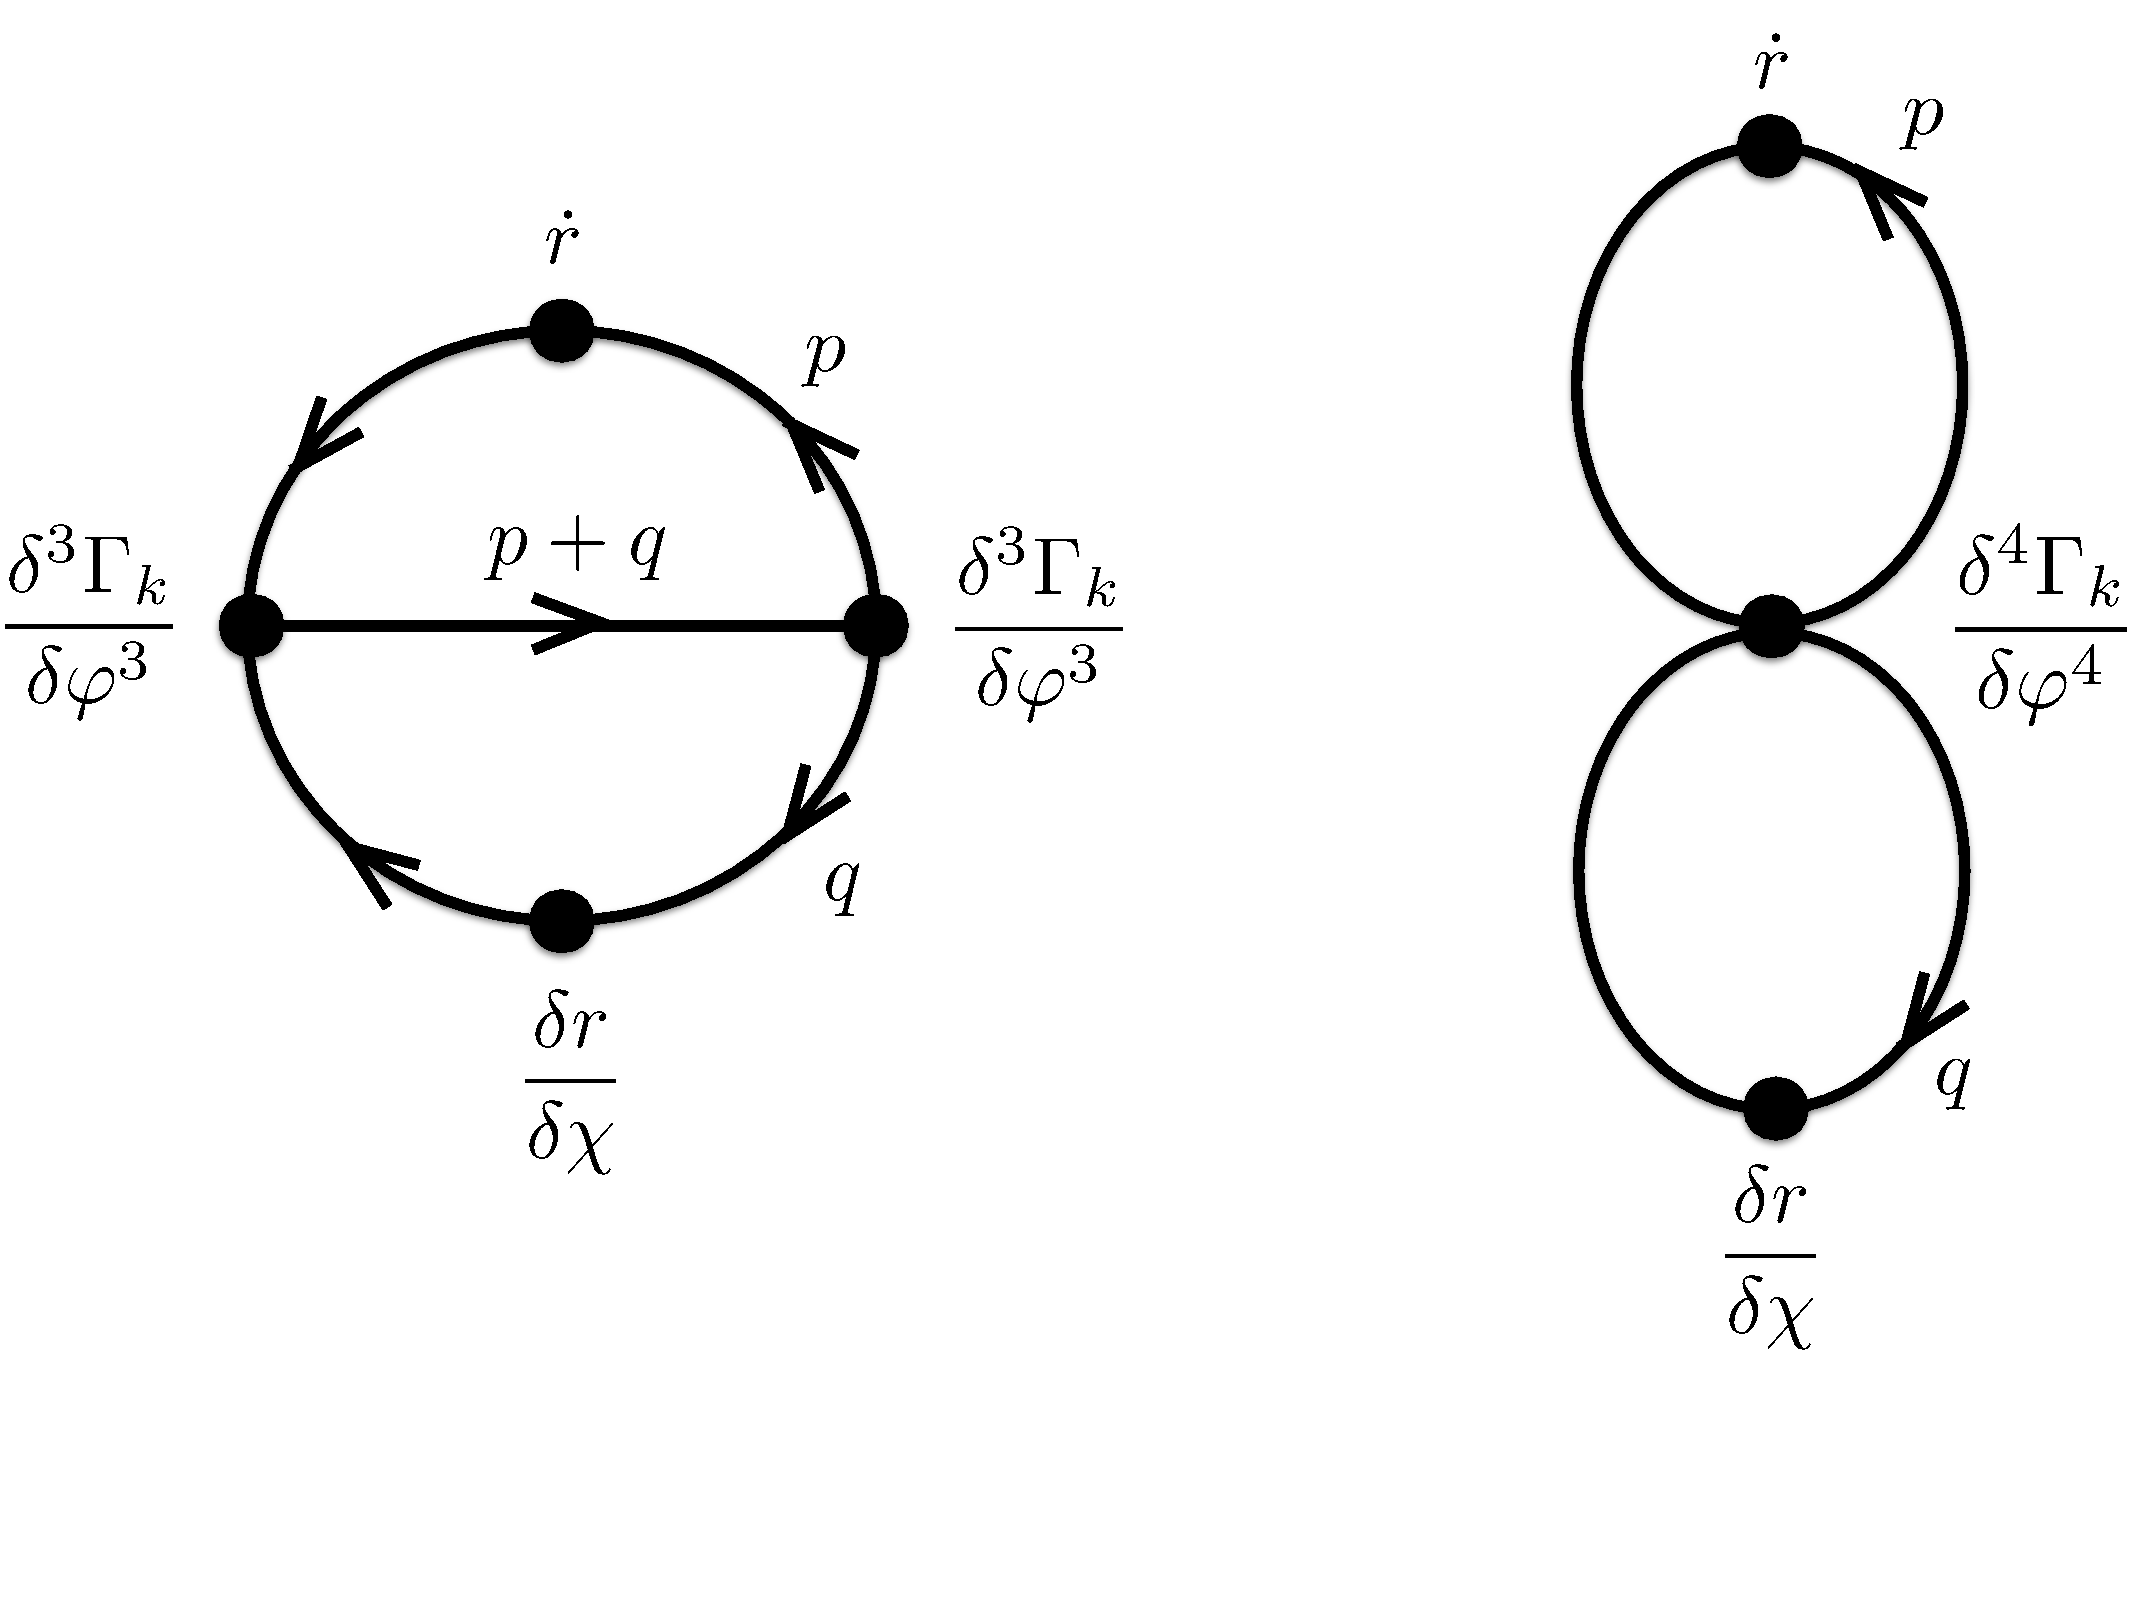
\includegraphics[scale=0.23]{two-loop.pdf}
\vskip-30pt
\caption{The two-loop diagrams in \eqref{step1}. Their symmetry immediately implies the identity \eqref{step2}. Momentum flow is indicated in the case where the fluctuation field $\varphi$ is then set to zero.}
\label{fig:two-loop}
\end{figure}
Recalling from \eqref{new-inverse} that $\Delta$ is an infrared regulated full propagator, we see from \eqref{step1} that the identity \eqref{step2} can be understood diagrammatically in terms of two-loop diagrams as sketched in fig. \ref{fig:two-loop}.
The symmetry of these diagrams means that nothing changes if we exchange $\dot{r}\leftrightarrow\delta r/\delta\chi$. This exchange immediately leads to the identity \eqref{step2}.


This identity breaks down in general in the derivative expansion.
If the Ward identity is approximated by a derivative expansion,
the full propagator in the one-loop term in \eqref{cal-W} is also expanded in a derivative expansion.
This full propagator has loop momentum $q$ say,
and is then expanded in powers of momenta carried by the external fluctuation
field $\varphi(p)$, \ie by the external legs.
The RG time derivative of the Ward identity yields the RG time derivative of such vertices,
as can be seen from the $\delta^2\dot{\Gamma}_k/\delta\varphi^2$ term  in \eqref{WIdot}.
This latter term has two internal legs given by the explicit functional derivatives,
carrying the loop momentum $q$ and joining full internal propagators $\Delta$,
and any number of external legs contained in the vertices of $\dot{\Gamma}_k$.
Substituting the flow equation \eqref{flow1} then gives in particular the last term in
eqn. \eqref{WIdot-2} in which two of these external legs are now joined to form a loop
connected via $\dot{r}$.  However it is momenta external to \emph{this new loop} which are
Taylor expanded in the derivative expansion of the flow equation
(see also \cite{Morris:1999ba, Morris:2000hm}).
This is illustrated in the diagram displayed in fig. \ref{fig:two-loop}.
In particular when the remaining external fluctuation field dependence is removed by setting $\varphi=0$,
we have exactly the momentum dependence displayed in the figure.
We see that a derivative expansion of the Ward identity involves Taylor expanding in small $p$,
while integrating over $q$.
However a derivative expansion of the flow equation involves Taylor expanding in small $q$,
and integrating over $p$ instead.
Thus the symmetry between the two loops is broken and the identity \eqref{step2} no longer follows.

On the other hand we see that if $\dot{r}$ and $\delta r/\delta\chi$ have the same momentum
dependence then the identity \eqref{step2} is restored because it is no longer possible
to distinguish the two loops.
Returning the placement of $\sqrt{\bar{g}}$ from \eqref{odd-r} to the integration measure,
this in fact would give us the relation \eqref{same-p-dependence} that is necessary and
sufficient for compatibility of the Ward identities within the derivative expansion,
and which we will now derive directly within the derivative expansion.


\subsection{Compatibility at order derivative-squared}\label{sec:compatibility-at-d2}

We now proceed to calculate the flow of the msWI for the system truncated at $\mathcal{O}(\partial^2)$ as described in sec. \ref{sec:review},
and investigate directly under which circumstances it vanishes. Let us start by writing the flow equations and msWIs for both $V$ and $K$ in the following form so that we can study both cases simultaneously:
\begin{align}
	\label{flowA}
	\dot A(\varphi,\chi) &= \int_p B_p\dot R_p \,,\\
	\label{msWIA}
	\mathcal{W}^{(A)}&=\bar\partial A - \gamma A + \int_p B_p(\partial_\chi R_p + \gamma R_p)=0 \,,
\end{align}
where $A$ is either $V$ or $K/f$ such that $B_p$ is either $Q_p$ or $2 P_p$ respectively. Here we have also introduced the shorthand notation
\be \label{gamma}
\int_p \equiv f(\chi)^{-\frac{d}{2}}\int dp \,p^{d-1}\,,\qquad \gamma \equiv \frac{d}{2}\partial_\chi \text{ln}f\,,\qquad{\rm and}\qquad \bar\partial \equiv \partial_\varphi - \partial_\chi\,.
\ee
It will also be useful to have to hand the following relations:
\begin{align}
	\label{DV}
	\left( \bar \partial + \partial_t - \gamma \right) V &=
	\mathcal W^{(V)} + \int_q Q_q (\dot R_q - \partial_{\chi} R_q - \gamma R_q)\,,\\
	\label{DK}
	\left( \bar \partial + \partial_t - \gamma \right) \frac{K}{f} &=
	\mathcal W^{(K)} + 2 \int_q P_q (\dot R_q - \partial_{\chi} R_q - \gamma R_q)\,,\\
	\label{DQ}
	\left( \bar \partial + \partial_t + n \gamma \right) Q_p^n &=
	-n \, \, Q_p^{n+1} \int_q (\partial_{\varphi}^2 Q_q - 2 \, p^2 P_q)(\dot R_q - \partial_{\chi} R_q
	 - \gamma R_q)\nonumber\\
	&\qquad-n \, Q_p^{n+1} (\dot R_p - \partial_{\chi} R_p - \gamma R_p)
	-n \, Q_p^{n+1} (\partial_{\varphi}^2 \mathcal W^{(V)} - p^2 \mathcal W^{(K)}).
\end{align}
The first two relations are derived by subtracting the msWI from the flow equation for $V$ and $K/f$ respectively.   The last relation is then derived by using the first two relations above together with the definition of $Q_p$ given in \eqref{Q}.

We begin by taking the RG time derivative of \eqref{msWIA}. Substituting in the flow equation for $\dot A$, and remembering the power of $f(\chi)$ hidden in the integral over $p$, this gives
\begin{equation}
	\label{flowWA1}
	\dot{ \mathcal W } ^ {(A)} =
 	\int_p \dot R_p \left( \bar\partial + \partial_t + \gamma \right) B_p
 	- \int_p \dot B_p \left( \dot R_p - \partial_{\chi} R_p - \gamma R_p \right) .
\end{equation}
In order to proceed we have to assume a particular form of $B_p$ so that we can compute the result of the linear operators under the integral acting on it. A general term in $P_p$ takes the form
\begin{equation}
	\tilde B_p =
 	\left( \partial_{\varphi}^i V \right) ^ a
 	\left( \partial_{\varphi}^j \frac{K}{f} \right) ^ b
 	\left( \partial_{p^2}^k R_p \right) ^ c \left(p^2\right)^l Q_p^e \,,
\end{equation}
where $a,b,c,e,i,j,$ $k$ (not to be confused with the cutoff scale), and $l$ are non-negative integers. From the structure of the terms in $P_p$ one can read off the following sum rule for the exponents:
\begin{equation}
	a+b+c = e-1 \,.
\end{equation}
Notice that the case $B_p = Q_p$  for the potential is also included, since  $a=b=c=l=0$ and $e=1$ also satisfies the sum rule.
Taking the term under the first integral of \eqref{flowWA1}, we find
\begin{align}
\nonumber
	\left( \bar\partial + \partial_t + \gamma \right) \tilde B_p &=
	\bigg[a \left( \partial_{\varphi}^i V \right) ^ {-1} \partial_{\varphi}^i \left(  \bar\partial + \partial_t \right) V
	+ b \left( \partial_{\varphi}^j \frac{K}{f} \right) ^ {-1} \partial_{\varphi}^j
	 \left(  \bar\partial + \partial_t \right) \frac{K}{f} \\
	&\quad+ c \left( \partial_{p^2}^k R_p \right) ^ {-1} \partial_{p^2}^k \left( - \partial_{\chi} + \partial_t \right) R_p
	+ e \, Q_p^{-1} \left( \bar\partial + \partial_t \right) Q_p+ \gamma\bigg ] \tilde B_p \,.
\end{align}
%Note that the effect of the inverses above is to remove from $\tilde B_p$ one such factor, which is then replaced with the same factor again but acted on by the first order differential operator  $ \bar\partial + \partial_t$.
Substituting equations \eqref{DV}--\eqref{DQ} into the above expression and using the sum rule, we obtain
\begin{align}
\label{DB}
	\nonumber
	\left( \bar\partial + \partial_t + \gamma \right) \tilde B_p &=
	\bigg[a \left( \partial_{\varphi}^i V \right) ^ {-1} \partial_{\varphi}^i \left(  \mathcal W^{(V)}
	 + \int_q Q_q \bar R_q \right)\\ \nonumber
	&\quad+ b \left( \partial_{\varphi}^j \frac{K}{f} \right) ^ {-1} \partial_{\varphi}^j \left(  \mathcal W^{(K)}
	+ 2 \int_q P_q \bar R_q \right)
	+ c \left( \partial_{p^2}^k R_p \right) ^ {-1} \partial_{p^2}^k \bar R_p \\
	&\quad- e\, Q_p \int_q \left( \partial_{\varphi}^2 Q_q - 2 p^2 P_q \right) \bar R_q
	- e\, Q_p \bar R_p
	- e\, Q_p \left( \partial_{\varphi}^2 \mathcal W^{(V)} - p^2 \mathcal W^{(K)} \right)
	 \bar R_q\bigg] \tilde B_p \,.
\end{align}
where we have introduced the shorthand notation
\be
\bar R_p = \dot R_p - \partial_\chi R_p - \gamma R_p\,.
\ee
Turning our attention now to the second integral of \eqref{flowWA1} we take the RG time derivative of $\tilde B_p$ and again substitute in the flow equations for $V$ and $K/f$. This gives
\begin{align}
\label{Bdot}
\nonumber
	\dot{ \tilde B }_p &=
	\bigg[	a \left( \partial_{\varphi}^i V \right) ^ {-1} \partial_{\varphi}^i \int_q Q_q \dot R_q
	+ b \left( \partial_{\varphi}^j \frac{K}{f} \right) ^ {-1} \partial_{\varphi}^j \int_q 2 P_q \dot R_q \\
	&\quad+ c \left( \partial_{p^2}^k R_p \right) ^ {-1} \partial_{p^2}^k \dot R_p
	- e \, Q_p \int_q  \left( \partial_{\varphi}^2 Q_q - 2 p^2 P_q \right) \dot R_q
	- e \, Q_p  \dot R_q\bigg] \tilde B_p  \,.
\end{align}
Inserting \eqref{DB} and \eqref{Bdot} into \eqref{flowWA1} we obtain
\begin{align}
\nonumber
 	\mathcal{\dot W}^{(A)} &= \sum_{\tilde B_p} \Bigg\{a \int_{p,q}
 	\tilde B_p ( \partial_{\varphi}^i V ) ^ {-1} \partial_{\varphi}^i
	\bigg( \dot R_p \mathcal{W}^{(V)} +Q_q [ \dot R , \partial_{\chi} R + \gamma R ]_{qp} \bigg) \\ \label{flowWA}
	&\quad+ b \int_{p,q} \tilde B_p \left( \partial_{\varphi}^j \frac{K}{f} \right) ^ {-1} \partial_{\varphi}^j
	\bigg( \dot R_p \mathcal{W}^{(K)} + 2 P_q [ \dot R , \partial_{\chi} R + \gamma R ]_{qp} \bigg) \\\nonumber
	&\quad+ c \int_p \tilde B_p \left( \partial_{p^2}^k R_p \right) ^ {-1}
	\left( \left(\partial_\chi R_p + \gamma R_p\right) \partial_{p^2}^k \dot R_p - \dot R_p \partial_{p^2}^k \left(\partial_\chi R_p + \gamma R_p\right) \right) \\ \nonumber
	&\quad- e \int_p \tilde B_p  Q_p  \dot R_p \bigg( \partial^2_{\varphi} \mathcal{W}^{(V)}
	 - p^2  \mathcal{W}^{(K)} \bigg)- e \int_{p,q}  \tilde B_p Q_p \bigg(  \partial_{\varphi}^2 Q_q
	 - 2 p^2 P_q \bigg) [ \dot R , \partial_{\chi} R + \gamma R ]_{qp}\Bigg\}\,,
\end{align}
where we have introduced the commutator-like construct $[A,B]_{qp} = A_q B_p - B_qA_p$.
%where $n$ labels each term in $P_p$ or $Q_p$ itself.

When $A = V$ the above expression simplifies considerably to
\begin{equation}
\label{flowWV}
	 \mathcal{\dot W}^{(V)}=-  \int_p  Q^2_p  \dot R_p\, \bigg( \partial^2_{\varphi} \mathcal{W}^{(V)}
	  - p^2  \mathcal{W}^{(K)} \bigg) - \int_{p,q}   Q^2_p\, \bigg(  \partial_{\varphi}^2 Q_q
	  - 2 p^2 P_q \bigg) [ \dot R , \partial_{\chi} R + \gamma R ]_{qp} \,,
\end{equation}
which we see contains only terms that contain either the Ward identities or the `commutator' $[ \dot R , \partial_{\chi} R + \gamma R ]_{qp}$. On the other hand for the flow of the $K/f$ msWI, the terms do not collect, so that it remains separately dependent on the individual $\tilde B_p$. However each term either contains the Ward identities themselves, the `commutator'  $[ \dot R , \partial_{\chi} R + \gamma R ]_{qp}$, or the additional commutator-like structures:
\be
\label{k-comm}
 \left(\partial_\chi R_p + \gamma R_p\right) \partial_{p^2}^k \dot R_p - \dot R_p \partial_{p^2}^k \left(\partial_\chi R_p + \gamma R_p\right)\,.
 \ee
These appear in the third line of \eqref{flowWA}, and the integer $k$ takes values $1$ and $2$. For a general cutoff $R_p$, these two additional commutator terms neither vanish nor combine with other terms of the flow.

If $[ \dot R , \partial_{\chi} R + \gamma R ]_{qp}$ vanishes, the flow \eqref{flowWV} of the V msWI is automatically satisfied providing that both the $K$ and $V$ msWI are also satisfied. In this case we have by rearrangement that
\be
\left( \partial_\chi R_p + \gamma R_p \right)/\dot R_p = \left( \partial_\chi R_q + \gamma R_q \right)/\dot R_q\,,
\ee
which means that the ratio is independent of momentum. Equivalently
\be
\label{same-p-dependence}
   \partial_\chi R_p + \gamma R_p = F(\chi,t) \,\dot R_p \,,
\ee
where $F$ can be a function of $\chi$ and $t$ but not of $p$.
However it is straightforward to see that \eqref{same-p-dependence} also forces the additional commutators \eqref{k-comm} to vanish.

We have therefore shown that all the commutator-like terms vanish if and only if $\dot R_p$ and $\partial_{\chi} R_p + \gamma R_p$ have the same dependence on $p$, with the consequence  that both the $\mathcal{\dot W}^{(A)}$ vanish, if the Ward identities $\mathcal{W}^{(A)}$ themselves vanish. Since for general choices of the functions, the vanishing of the `commutators' is surely necessary to achieve $\mathcal{\dot W}^{(A)}=0$ without further restriction, we have thus shown that the condition \eqref{same-p-dependence} is necessary and sufficient to ensure compatibility, as defined at the beginning of this section.


\subsection{Incompatibility implies no solutions}\label{sec:incompatibility}

However even if the commutators do not vanish, and thus the Ward identities are incompatible
with the flow equations, {\it a priori} there could still be a non-empty restricted set of solutions
that both satisfy the flow equations and Ward identities.
In this case the equations are satisfied not by the vanishing of the commutators themselves,
but by the fact that for the given solutions the sum of all these terms vanish after
performing the integration over momenta.
Therefore, as well as obeying the flow equations and the msWIs $\mathcal{W}^{(A)}=0$,
the solutions must also separately obey two further conditions,
namely the vanishing of the right hand sides of \eqref{flowWA}.
In the language of Dirac's classification of constraints \cite{dirac2001lectures, Dirac:1950pj},
the $\mathcal{W}^{(A)}=0$ provide the primary constraints.
We have shown that if the `commutators' do not vanish,
then the solutions are subject also to non-trivial secondary constraints $\mathcal{\dot W}^{(A)}=0$.
Given the involved form of $\mathcal{\dot W}^{(K)}$ in particular,
we can be sure that the procedure does not close and that actually there is then an infinite
tower of secondary constraints, $\partial^n_t \,\mathcal{W}^{(A)}=0,\;\forall \,n>0$,
all of which must be satisfied.
It would therefore seem inevitable that there are in fact no non-trivial solutions in this case.
We will confirm this by example in sec. \ref{sec:incompatible-no-solns}.
We conclude that \emph{the vanishing of the `commutators',
and hence condition \eqref{same-p-dependence},
is both necessary and sufficient for there to be any solutions to the flows and Ward identities
in the derivative expansion approximation outlined in sec. \ref{sec:review}}.

The condition \eqref{same-p-dependence} was already used in ref. \cite{Dietz:2015owa},
where however it was introduced as a mathematical trick to help solve the coupled system of
flow equations and msWI. As we recall below, it implies either that $\eta=0$ or $R_p$ is of power-law form.
We now see that the requirement for $\dot R_p$ and $\partial_{\chi} R_p + \gamma R_p$ to have the
same dependence on $p$, goes much deeper: the flow equations \eqref{flowV} and \eqref{flowK},
and the Ward identities \eqref{msWIV} and \eqref{msWIK}, are incompatible without this constraint,
and incompatibility forces there to be no solutions to the combined system.


\subsection{Required form of the cutoff profile}\label{sec:required-cutoff}

Note that $R_p$ must take a form that respects the scaling dimensions.
Introducing dimensionless variables for use in the next section and later,
we can make these scaling dimensions explicit by employing the RG scale $k$.
We denote the new dimensionless quantities with a bar.
We have
\begin{align}
\label{dim-vars}
	\varphi = k^{\eta/2}\bar\varphi, \qquad\chi = k^{\eta/2}\bar\chi, \qquad f(\chi) = k^{d_f}\bar f(\chi),\nonumber\\
	V(\varphi,\chi) = k^{d_V}\bar V(\bar\varphi,\bar\chi), \qquad K(\varphi, \chi) = k^{d_R- 2 + d_f} \bar  K(\bar\varphi,\bar\chi),
\end{align}
where
\be
\label{dimensions}
d_V = d(1-d_f/2)\qquad{\rm and}\qquad d_R = d_V - \eta\,,
\ee
and thus from \eqref{cutoff-action} and \eqref{conformal-reduction},
we have by dimensions that $R_p$ must take the form
\begin{equation}
\label{equ:cutoff}
	R(p^2/f)= - k^{d_R} \,r\left(\frac{p^2}{k^{2-d_f}f}\right) = - k^{d_R} \,r(\hat p^2) \,,
\end{equation}
where $r$ is a dimensionless cutoff profile of a dimensionless argument,\footnote{The minus sign in \eqref{equ:cutoff} is necessary to work with the wrong sign kinetic term in \eqref{trunc} \cite{Dietz:2015owa}.} and we have introduced the dimensionless momentum magnitude $\hat p = p\sqrt{k^{d_f-2}/f}$.

If $\dot R_p$ and $\partial_{\chi} R_p + \gamma R_p$ have the same dependence on $p$, \ie satisfy \eqref{same-p-dependence}, then either $\eta=0$ or $R_p$ is of power-law form \cite{Dietz:2015owa}. To see this, note that from \eqref{equ:cutoff} and \eqref{gamma} we have
\be
\label{R-scaling-relation}
\gamma {\dot R}_p = d_V \left[\partial_\chi R_p+\gamma R_p\right] -\eta \gamma R_p\,.
\ee
Thus (choosing $F=\gamma/d_V$) we see that \eqref{same-p-dependence} is satisfied if $\eta=0$, without further restriction on $R$. However if $\eta\ne0$, then \eqref{R-scaling-relation} together with \eqref{same-p-dependence} implies
%\be
%\eta \dclnf R_p = A  \left[\partial_\chi R_p+\frac{d}{2}\dclnf R_p\right]\,,
%\ee
%where $A$ can be a function of $\chi$ and $t$ but not $p$. Rearranging, we see that this implies
\be
f \frac{\partial R_p}{\partial f} = \frac{d}{2}\left( \frac{\eta F}{ d_VF- \gamma} - 1\right) R_p\,,
\ee
and thus from \eqref{equ:cutoff}
\be
\hat{p} \frac{d}{d\hat{p}} r(\hat{p}^2) = -d\left( \frac{\eta F}{ d_VF- \gamma} - 1\right) r(\hat{p}^2)\,.
\ee
Since the term in brackets does not depend on $p$, we see that this is only possible if in fact the term in brackets is a constant. Setting this constant to be $2n/d$ for some constant $n$, we thus also deduce that $r\propto \hat{p}^{-2n}$.

An example of a cutoff that does not satisfy \eqref{same-p-dependence} if $\eta\ne0$, and thus leads to incompatible msWIs in this case, is the optimised cutoff \cite{Litim:2000ci, Litim:2001fd}:
\be
\label{optimised}
r(\hat{p}^2) = (1-\hat{p}^2)\theta(1-\hat{p}^2)\,.
\ee
It is straight-forward to confirm that this does not satisfy \eqref{same-p-dependence} if $\eta\ne0$. Using \eqref{equ:cutoff} and \eqref{R-scaling-relation} we find
\be
\dot{R}_p \propto d_V \left[ \frac{2}{d}\,\theta(1-\hat{p}^2) + (1-\hat{p}^2)\theta(1-\hat{p}^2)\right] - \eta\, (1-\hat{p}^2)\theta(1-\hat{p}^2)\,.
\ee
In order for \eqref{optimised} to satisfy \eqref{same-p-dependence}, the right hand side must be proportional to $\partial_\chi R_p+\gamma R_p$ \ie to the term in square brackets. This is only true if $\eta=0$.


\section{LPA equations}

We will now use the Local Potential Approximation to further investigate the restriction imposed by the msWI on the RG flow equation, in terms of general solutions and also on the existence of $k$-fixed points (\ie RG fixed points with respect to variations in $k$). We start with a very clear example where the msWI forbids the existence of $k$-fixed points.

Then using the concrete example of the optimised cutoff we show explicitly that compatibility forces $\eta=0$ for non-power-law cutoffs. Setting $\eta=0$ we will see that background independent variables exist, in other words they exist whenever the msWI is compatible with the flow. We will also see that such $\hat{k}$-fixed points coincide with the $k$-fixed points. The background independent variables allow us to solve for the fixed points explicitly, uncovering a line of fixed points, consistent with the findings for power-law cutoff \cite{Dietz:2016gzg}.

\subsection{Demonstration of background independence forbidding fixed points in general}\label{sec:forbids}

We use the change to dimensionless variables \eqref{dim-vars} and \eqref{equ:cutoff}. In the LPA we discard the flow and Ward identity for $K$, and set $\bar K=1$. The result, for general cutoff profile $r(\hat{p}^2)$, is:
\begin{align}
\label{flow}
\partial_t \bar V + d_V \bar V - \frac{\eta}{2} \, \bar\varphi \, \frac{\partial \bar V}{\partial \bar\varphi} - \frac{\eta}{2} \, \bar\chi \, \frac{\partial \bar V}{\partial \bar\chi} &=
\int_0^{\infty} d\hat p \, \hat p^{d-1} \, \frac{d_R\, r - \frac{d_V}{d} \, \hat p \, r'}{\hat p^2 + r - \partial^2_{\bar\varphi}\bar V}\,,\\
\label{msWI}
\frac{\partial \bar V}{\partial \bar\chi} - \frac{\partial \bar V}{\partial \bar\varphi} + \bar \gamma \, \bar V &= \bar \gamma
\int_0^{\infty} d\hat p \, \hat p^{d-1} \, \frac{r - \frac{1}{d} \, \hat p \, r'}{\hat p^2 + r - \partial^2_{\bar\varphi}\bar V} \,,
\end{align}
where $r'$ means $dr(\hat{p}^2)/d\hat{p}$ and from the change to dimensionless variables we find:
\be
\label{fbar-general}
\bar{\gamma} = \frac{d}{2}\frac{\partial}{\partial\bc}\ln\bar{f}\left({\rm e}^{\eta t/2}\mu^{\eta/2}\bc\right)\,.
\ee
Note that since $f$ cannot depend on $t$ (see the discussion in sec. \ref{sec:review}), once we go to dimensionless (\ie scaled) variables, $\bar{f}$ is in general forced to depend on $t$ if $\chi$ has non-vanishing scaling dimension $\eta$.
At the ($k$-)fixed point we must have $\partial_t \bar V = 0$. We see at once why fixed points are generically forbidden by the msWI: the fixed point potential $\bar{V}$ would have to be independent of $t$, but through \eqref{msWI} and \eqref{fbar-general} this is impossible in general since $\bV$ is forced to be dependent on explicit $t$-dependence in $\bar{f}$ through the Ward identity. This is true even in the case of power-law cutoff profile\footnote{And indeed this issue was highlighted, but in a different way in ref. \cite{Dietz:2015owa}.} which as we have seen allows \eqref{msWI} to be compatible with the flow \eqref{flow}.



At first sight an escape from this problem is simply to set $f$ to be power law.
Indeed setting $f\propto\chi^{\rho}$ for some constant $\rho$, \eqref{fbar-general} implies
\be
\bg = \frac{d}{2} \frac{\rho}{\bc}\,,
\label{powlaw-gamma}
\ee
and thus \eqref{msWI} no longer has explicit $t$ dependence.
Recall that for power-law cutoff profiles $r$, it was indeed found that $k$-fixed points for $\bV$
are allowed if $f$ is chosen of power law form \cite{Dietz:2015owa}.\footnote{This is true also for $\bar{K}$. However if the dimensions of $f$ and $\chi$ do not match up, these fixed points do not agree with
the background independent $\hat{k}$-fixed points and furthermore the effective action
$\Gamma_k$ still runs with $k$ \cite{Dietz:2015owa}.}
However we have seen in sec. \ref{sec:required-cutoff} that any other cutoff profile does
not allow the Ward identity to be compatible with the flow unless $\eta=0$.
We argued in sec. \ref{sec:incompatibility} that incompatibility overconstrains the equations
leading to no solutions. In the next subsection, sec. \ref{sec:incompatible-no-solns},
we will confirm this explicitly, choosing as a concrete example the optimised cutoff profile and
space-time dimension $d=4$.

On the other hand, if we set $\eta=0$ then the msWI \eqref{msWI} is compatible with the flow \eqref{flow},
for any parametrisation $f$. Apparently $k$-fixed points are also now allowed without further restriction,
since again \eqref{fbar-general} loses its explicit $t$ dependence.
Opting once more for optimised cutoff profile and $d=4$, we will see in sec. \ref{sec:works} that
indeed they are allowed and furthermore they coincide with fixed points in a background independent
description that we also uncover.


\subsection{Confirmation of no solutions if the msWI is incompatible with the flow}
\label{sec:incompatible-no-solns}

Specialising to optimised cutoff and (for simplicity) the most interesting case of spacetime dimension $d=4$,
the equations read
\begin{align}
\label{flowComplete_opt}
\partial_t\bar{V}+
d_V \bar V - \frac{\eta}{2} \bar \varphi \, \partial_{\bar\varphi}\bar V -\frac{\eta}{2} \bar \chi \, \partial_{\bar\chi}\bar V &= \left(  \frac{d_R}{6} + \frac{\eta}{12} \right) \frac{1}{1 -  \partial^2_{\bar\varphi}\bar V},\\
\label{msWI_opt}
\partial_{\bar\chi}\bar V - \partial_{\bar\varphi}\bar V + \bar{\gamma} \bar V &= \frac{\bar{\gamma}}{6} \frac{1}{1 - \partial^2_{\bar\varphi}\bar V}\,.
\end{align}
Choosing power law $f$ and thus \eqref{powlaw-gamma} there is no explicit $t$ dependence and apparently these equations can work together. Combining them by eliminating their right hand sides, we get
\be
\label{pde1}
2\partial_t\bar{V}+\eta\bar{V}-\left(\eta\bar\varphi-\alpha\bc\right)\partial_{\bar{\varphi}}\bar{V}-(\eta+\alpha)\bar\chi\partial_{\bar{\chi}} \bar{V}=0\,,
\ee
where we have introduced the constant $\alpha = (d_R+\eta/2)/\rho$.
This equation can be solved by the method of characteristics (see \eg the appendix in ref. \cite{Dietz:2015owa}). Parametrising the characteristic curves with $t$, they are generated by the following equations:
\be
\frac{d\bV}{dt} = -\frac{\eta}{2}\bV\,,\quad\frac{d\bc}{dt}=-\frac{\alpha+\eta}{2}\bc\,,\quad \frac{d\bp}{dt}=\frac{\alpha\bc-\eta\bp}{2}\,.
\ee
Solving the second equation before the third, it is straightforward to find the curves:
\be
\bV = \hV {\rm e}^{-\eta t/2}\,,\quad \bc = \hc\, {\rm e}^{-(\eta+\alpha)t/2}\,,\quad \bp+\bc = \hp\, {\rm e}^{-\eta t/2}\,,
\ee
in terms of initial data $\hV,\hp,\hc$.
Thus the solution to \eqref{pde1} can be written as
\be
\bV ={\rm e}^{-\eta t/2}\, \hV(\hp,\hc) ={\rm e}^{-\eta t/2} \,\hV\left({\rm e}^{\eta t/2}[\bp+\bc],{\rm e}^{(\eta+\alpha)t/2}\bc\right)\,,
\ee
as can be verified directly. Plugging this into either \eqref{flowComplete_opt} or \eqref{msWI_opt} gives the same equation, which in terms of the hatted variables reads
\be
\hc \partial_{\hc}\hV+2\rho\hV = \frac{\rho}{3}\frac{1}{{\rm e}^{-\frac{\eta}{2} t} \,-\partial^2_{\hp}\hV}\,.
\ee
Since $\hV(\hp,\hc)$ is independent of $t$, we see there are no solutions unless $\eta=0$.
%In other words, from sec. \ref{sec:required-cutoff}, there are no solutions unless the equations are compatible.
We saw in sec. \ref{sec:required-cutoff} that this was also the necessary and sufficient condition for compatibility in this case.

\subsection{Background independence at vanishing anomalous dimension}\label{sec:works}
We now set $\eta=0$. As recalled in sec. \ref{sec:required-cutoff}, the msWI is now compatible with the flow, and furthermore  from \eqref{fbar-general} the explicit $t$ dependence has dropped out.
%Setting $\eta=0$, at first sight there is now no problem with the equations \eqref{flowComplete_opt} and \eqref{msWI_opt} for any parametrisation $f$. As recalled in sec. \ref{sec:required-cutoff}, the msWI is compatible with the flow if $\eta=0$.  Furthermore, f
For power-law cutoff profiles we found that $k$-fixed points exist and coincide with background independent $\hk$-fixed points for any form of $f$ with any dimension $d_f$ \cite{Dietz:2015owa}. We will see that for non-power law cutoff that the same is true. (Again we choose optimised cutoff and $d=4$ as an explicit example.) We will uncover consistent background independent variables for which the full line of fixed points is visible \cite{Dietz:2016gzg}.

Since $\eta=0$, in the equations \eqref{flowComplete_opt} and \eqref{msWI_opt}, we also have $d_R=d_V=2(2-d_f)$ and $\bar{\gamma}=2\partial_{\bc}\ln\bar{f}(\bc)$. Note that from \eqref{equ:cutoff}, $d_f=2$ is excluded otherwise the IR cutoff no longer depends on $k$. Also note that since $\eta=0$ we can drop the bars on $\chi$ and $\vp$.
Combining the equations into a linear partial differential equation we get
\be
\label{pde2}
\partial_t\bV +\frac{2-d_f}{\partial_{\chi}\ln\bar{f}}\left(\partial_{\vp}\bV-\partial_{\chi}\bV\right) =0\,,
\ee
whose characteristic curves satisfy
\be
\label{eta0curves}
\frac{d\chi}{dt}=\frac{d_f-2}{\partial_{\chi}\ln\bar{f}}\,,\quad\frac{d\vp}{dt}=\frac{2-d_f}{\partial_{\chi}\ln\bar{f}}\,,\quad \frac{d\bV}{dt}=0\,.
\ee
Solving the first equation gives:
\be
\label{hatt}
\hatt = t+\frac{\ln\bar{f}}{2-d_f}\,,
\ee
where the integration constant $\hatt$ is thus the background independent definition of RG time (see the appendix to ref. \cite{Dietz:2015owa}). Exponentiating,
\be
\hk = k \left\{\bar{f}(\chi)\right\}^{\frac{1}{2-d_f}} = k^{2\frac{1-d_f}{2-d_f}} \left\{f(\chi)\right\}^{\frac{1}{2-d_f}}\,,
\ee
where the second equality follows from \eqref{dim-vars}. The sum of the first two equations in \eqref{eta0curves} tells us that $\phi=\vp+\chi$ is an integration constant for the characteristics, and finally the last equation says that $\bV$ is also constant for characteristics. Thus we learn that the change to background independent variables is achieved by writing
\be
\label{background-independent}
\bV = \hV(\phi,\hatt\,)\,.
\ee
It is straightforward to verify that this solves \eqref{pde2}. Substituting into either \eqref{flowComplete_opt} or \eqref{msWI_opt} gives the same flow equation:
\be
\label{bi-flow}
\partial_{\hatt}\hV +d_V\hV = \frac{d_V}{6}\frac{1}{1-\partial^2_\phi\hV^{\vphantom{H^H}}}\,,
\ee
which is indeed now background independent, \ie independent of $\chi$, and indeed independent of parametrisation $f$. There remains a dependence on the dimension of $f$ through $d_V = 2(2-d_f)$ although this disappears for $\hk$-fixed points, and can be removed entirely by a rescaling $\hatt\mapsto \hatt\, d_V$ which however changes the dimension of $\hat{k}$ to $d_V$.

We also see from \eqref{hatt} and \eqref{background-independent} that
\be
\partial_t \bV = \partial_{\hatt} \hV\,,
\ee
and thus fixed points in $k$ coincide with the background independent fixed points.

Finally, the fixed points are readily found from \eqref{bi-flow} similarly to refs. \cite{Dietz:2016gzg,Morris:1994jc} by recognising that
\be
\frac{d^2\hV}{d\phi^2} = 1-\frac{1}{6\hV}
\ee
is equivalent to Newton's equation for acceleration with respect to `time' $\phi$ of a particle of unit mass at `position' $\hV$ in a potential $U=-\hV+ (\ln\hV)/6$. In this way it can be verified that there is a line of fixed points ending at the Gaussian fixed point, which is here $\hV=1/6$, in agreement with the findings for power-law cutoff in \cite{Dietz:2016gzg}.





\section{Polynomial truncations}
\label{sec:truncations}

The analysis  so far has used properties of conformally truncated gravity and the derivative expansion approximation method. In order to gain insight about what might happen at the non-perturbative level, and in full quantum gravity, we will consider how the issues would become visible in polynomial truncations.

The generic case treated in sec. \ref{sec:forbids} will be just as clear in the sense that truncations of the Ward identity will still force the effective potential (effective action in general) to be $t$ dependent if the dimensionless parametrisation \eqref{fbar-general} is similarly forced to be $t$ dependent. In general therefore, if the way the metric is parametrised forces the parametrisation to become $t$ dependent, we can expect that background independence excludes the possibility of fixed points, at least with respect to $t$.


Consider next the situation treated in sec. \ref{sec:incompatible-no-solns}. Expanding the dimensionless potential and the equations in a double power series in the fluctuation and the background field, we write:
\begin{equation}
\label{pot-expand}
\bar V(\bar\varphi,\bar\chi) = \sum_{n,m=0}^{\infty} a_{nm} \bar\varphi^n \bar\chi^m\,.
\end{equation}
Substituting \eqref{powlaw-gamma} into \eqref{msWI_opt} and multiplying through by $\bc$, we can read off from this and \eqref{flowComplete_opt} the zeroth level equations:
\be
d_V a_{00} = \left(  \frac{d_R}{6} + \frac{\eta}{12} \right) \frac{1}{1 -  2a_{20}}\,,\qquad 2\rho\, a_{00} = \frac{\rho}{3} \frac{1}{1 -  2a_{20}}\,.
\ee
Since $\rho$ cannot vanish and $a_{20}$ cannot diverge, combining these equations gives $d_V = d_R+\eta/2$ which from \eqref{dimensions} implies $\eta=0$. Thus we recover already from the zeroth order level that fixed points are excluded unless $\eta=0$. (Of course the real reason, namely that the equations are incompatible, and the full consequence that there are no $t$-dependent solutions either, is maybe not so easy to see this way.)

\subsection{Counting argument}\label{sec:counting}

%For other cases we expand the dimensionless potential and the equations in a double power series in the fluctuation and the background field
%and then count the resulting number of coefficients and equations.

We already argued in the Introduction, that generically the coefficients become overconstained if we consider a sufficiently high truncation. We now proceed to make a careful count and estimate the level at which this happens.




We concentrate on fixed point solutions to the LPA system \eqref{flow}, \eqref{msWI} and \eqref{fbar-general} where either $\eta=0$ or we choose power-law $f$, so that explicit $t$ dependence does not already rule out such solutions. We introduce the short-hand notation $\bar V ^{(n,m)}=\partial_{\bar \varphi}^n \partial_{\bar \chi}^m \bar V(\bp,\bc)$.
To obtain the system at order $r$ we have to plug the expansion of the potential \eqref{pot-expand}
%\begin{equation}
%\bar V(\bar\varphi,\bar\chi) = \sum_{n,m=0}^{\infty} a_{nm} \bar\varphi^n \bar\chi^m\,
%\end{equation}
into both the fixed point equation and msWI, act on them with operators $\frac{\partial^{i+j}}{\partial \bar\varphi^i \, \partial \bar\chi^j}$ such that $i+j=r$, before finally setting the fields to zero. In particular, for any fixed value $r_{\star}$ we have $2 \, (r_{\star}+1)$ equations
%\footnote{%
%Here we assume that the flow equation and the msWI are independent of each other at every order.
%}
and hence up to order $r$ there are
\begin{equation}
\label{number_eqns}
n_{\text{eqn}}(r) = \sum_{i=0}^{r} 2\,(i+1) = r^2 + 3r + 2
\end{equation}
equations.

To count the coefficients appearing in these $n_{\text{eqn}}(r)$ equations let us start with the left hand sides. First note that
\begin{equation}
\label{proportionality}
\bar V^{(i,j)} \bigg|_{\bar\varphi = \bar\chi = 0}
\propto a_{ij} \,.
\end{equation}
That is, for any fixed pair $(i,j)$ the left hand side of (\ref{msWI}) will contain the coefficients $a_{ij}$, $a_{i+1,j}$ and $a_{i,j+1}$, whereas the left hand side of (\ref{flow}) will only contain $a_{ij}$. Up to some fixed order $r$ there will be thus coefficients $a_{ij}$ where $i$ and $j$ run from $0$ to $r+1$ and $i+j \leqslant r+1$
%%%%%%%%%%%%%%%%%%%%%%%%%%%%%%%%%%%%%%%%%%%%%%%%%
\begin{figure}
\centering
\begin{tikzpicture}[>=stealth]
\draw (0,0) -- (1,0) -- (1,-1) -- (0,-1) -- cycle;
\draw (1,0) -- (2,0) -- (2,-1) -- (1,-1) -- cycle;
\draw (2,0) -- (3,0) -- (3,-1) -- (2,-1) -- cycle;
\draw (3,0) -- (4,0) -- (4,-1) -- (3,-1) -- cycle;

\draw (0,-1) -- (1,-1) -- (1,-2) -- (0,-2) -- cycle;
\draw (1,-1) -- (2,-1) -- (2,-2) -- (1,-2) -- cycle;
\draw (2,-1) -- (3,-1) -- (3,-2) -- (2,-2) -- cycle;

\draw (0,-2) -- (1,-2) -- (1,-3) -- (0,-3) -- cycle;
\draw (1,-2) -- (2,-2) -- (2,-3) -- (1,-3) -- cycle;

\draw (0,-3) -- (1,-3) -- (1,-4) -- (0,-4) -- cycle;

\draw (0.5,0.5) node {0}  (1.5,0.5) node {1}  (2.5,0.5) node {$\cdots$} (3.5,0.5) node {$r+1$};
\draw (-0.5,-0.5) node {0}  (-0.5,-1.5) node {1}  (-0.5,-2.5) node {$\vdots$} (-0.5,-3.5) node {$r+1$};

\draw (0.5,-0.5) node {$a_{00}$}  (1.5,-0.5) node {$a_{01}$}
(2.5,-0.5) node {$\cdots$}  (3.5,-0.5) node {$a_{0,r+1}$};
\draw (0.5,-1.5) node {$a_{10}$}  (1.5,-1.5) node {$\ddots$};
\draw (0.5,-2.5) node {$\vdots$};
\draw (0.5,-3.5) node {$a_{r+1,0}$};

\draw (-0.25,0.5) node {$j$} (-0.5,0.25) node {$i$};
\draw (-0.15,0.15) -- (-0.55,0.55);
\end{tikzpicture}
\caption{Coefficients of the potential appearing on the left sides of the equations.}
\label{diag_lhs}
\end{figure}
%%%%%%%%%%%%%%%%%%%%%%%%%%%%%%%%%%%%%%%%%%%%%%
\begin{equation}
\label{coeff_lhs}
\bigg\lbrace a_{00}, a_{01}, \dots , a_{0,r+1}, a_{10}, \dots , a_{1,r}, \dots , a_{2,r-1}, \dots, a_{r+1,0}   \bigg\rbrace \,,
\end{equation}
 (cf. figure \ref{diag_lhs}). This adds up to the following number of coefficients
\begin{equation}
n_{\text{lhs}}(r) = \sum_{i=1}^{r+2} \, i = \frac{1}{2} \, r^2 + \frac{5}{2} \, r + 3 \,.
\end{equation}

Including the coefficients of the right hand side, we have to be careful not to double count any coefficients that have already been taken account of on the left hand sides. Let us suppose we have fixed the cutoff and let us assume that for the moment $\bar{\gamma} =$ const. Then all additional coefficients on the right hand side come from the expansion of the propagator
\begin{equation}
\label{expansion_propagator}
\frac{\partial^{i+j}}{\partial \bar\varphi^i \, \partial \bar\chi^j} \, \left( \frac{1}{1 - \bar V^{(2,0)}} \right) \bigg|_{\bar\varphi = \bar\chi = 0} =
\frac{\partial^{j}}{\partial \bar\chi^j} \left[ \frac{\partial^{i-1}}{\partial \bar\varphi^{i-1}} \left( \frac{\bar V^{(3,0)}}{(1 - \bar V^{(2,0)})^2} \right) \right] \bigg|_{\bar\varphi = \bar\chi = 0}\, .
\end{equation}
Since we can always arrange the $\bar\varphi$--derivatives to act first, the expression in the square brackets will involve terms $\bar V^{(2,0)} \cdots \, \bar V^{(i+2,0)}$. Using (\ref{proportionality}), we see that the expression given in (\ref{expansion_propagator}) will then include terms
\begin{equation}
\bigg\lbrace a_{20}, a_{21}, \dots , a_{2i}, a_{30}, \dots , a_{3i}, \dots, a_{i+2,0}, \dots, a_{i+2,j}   \bigg\rbrace \,.
\end{equation}
Up to any fixed order $r$, $i$ and $j$ can take values between $0$ and $r$ such that $i+j = r$, and in total we will have the following coefficients on the right hand sides
%%%%%%%%%%%%%%%%%%%%%%%%%%%%%%%%%%%%%%%%%%%%%%
\begin{figure}
\centering
\begin{tikzpicture}[>=stealth]
\draw (0,0) -- (1,0) -- (1,-1) -- (0,-1) -- cycle;
\draw (1,0) -- (2,0) -- (2,-1) -- (1,-1) -- cycle;
\draw (2,0) -- (3,0) -- (3,-1) -- (2,-1) -- cycle;
\draw (3,0) -- (4,0) -- (4,-1) -- (3,-1) -- cycle;

\draw (0,-1) -- (1,-1) -- (1,-2) -- (0,-2) -- cycle;
\draw (1,-1) -- (2,-1) -- (2,-2) -- (1,-2) -- cycle;
\draw (2,-1) -- (3,-1) -- (3,-2) -- (2,-2) -- cycle;

\draw (0,-2) -- (1,-2) -- (1,-3) -- (0,-3) -- cycle;
\draw (1,-2) -- (2,-2) -- (2,-3) -- (1,-3) -- cycle;

\draw (0,-3) -- (1,-3) -- (1,-4) -- (0,-4) -- cycle;

\draw (0.5,0.5) node {0}  (1.5,0.5) node {1}  (2.5,0.5) node {$\cdots$} (3.5,0.5) node {$r$};
\draw (-0.5,-0.5) node {2}  (-0.5,-1.5) node {3}  (-0.5,-2.5) node {$\vdots$} (-0.5,-3.5) node {$r+2$};

\draw (0.5,-0.5) node {$a_{20}$}  (1.5,-0.5) node {$a_{21}$}
(2.5,-0.5) node {$\cdots$}  (3.5,-0.5) node {$a_{2,r}$};
\draw (0.5,-1.5) node {$a_{30}$}  (1.5,-1.5) node {$\ddots$};
\draw (0.5,-2.5) node {$\vdots$};
\draw (0.5,-3.5) node {$a_{r+2,0}$};

\draw (-0.25,0.5) node {$j$} (-0.5,0.25) node {$i$};
\draw (-0.15,0.15) -- (-0.55,0.55);
\end{tikzpicture}
\caption{Coefficients of the potential appearing in the expansion of the propagator.}
\label{diag_rhs}
\end{figure}
%%%%%%%%%%%%%%%%%%%%%%%%%%%%%%%%%%%%%%%%%%%%%%%%
\begin{equation}
\bigg\lbrace a_{20}, \dots , a_{2,r}, a_{30}, \dots , a_{3,r-1}, \dots , a_{4,r-2}, \dots, a_{r+2,0}   \bigg\rbrace \,,
\end{equation}
(cf. figure \ref{diag_rhs}). Most of these coefficients have however already been accounted for on the left hand sides c.f. (\ref{coeff_lhs}). The only ones not counted yet are
%%%%%%%%%%%%%%%%%%%%%%%%%%%%%%%%%%%%%%%%%%%%%%%
\begin{figure}
\centering
\begin{tikzpicture}[>=stealth]
\foreach \i in {0,...,6} {
\draw[pattern=north east lines] (0+\i,0) rectangle (1+\i,-1); }

\foreach \i in {0,...,5} {
\draw[pattern=north east lines] (0+\i,-1) rectangle (1+\i,-2); }

\foreach \i in {0,...,4} {
\draw[pattern=crosshatch] (0+\i,-2) rectangle (1+\i,-3); }
\draw[pattern=north west lines] (5,-2) rectangle (6,-3);

\foreach \i in {0,...,3} {
\draw[pattern=crosshatch] (0+\i,-3) rectangle (1+\i,-4); }
\draw[pattern=north west lines] (4,-3) rectangle (5,-4);

\foreach \i in {0,...,2} {
\draw[pattern=crosshatch] (0+\i,-4) rectangle (1+\i,-5); }
\draw[pattern=north west lines] (3,-4) rectangle (4,-5);

\foreach \i in {0,...,1} {
\draw[pattern=crosshatch] (0+\i,-5) rectangle (1+\i,-6); }
\draw[pattern=north west lines] (2,-5) rectangle (3,-6);

\draw[pattern=crosshatch] (0,-6) rectangle (1,-7);
\draw[pattern=north west lines] (1,-6) rectangle (2,-7);
\draw[pattern=north west lines] (0,-7) rectangle (1,-8);

\draw (0.5,0.5) node {0}  (1.5,0.5) node {1}  (2.5,0.5) node {2} (3.5,0.5) node {$\cdots$}
(4.5,0.5) node {$r-1$}  (5.5,0.5) node {$r$}  (6.5,0.5) node {$r+1$};
\draw (-0.5,-0.5) node {0}  (-0.5,-1.5) node {1}  (-0.5,-2.5) node {2} (-0.5,-3.5) node {$\vdots$}
(-0.5,-4.5) node {$r-1$}  (-0.5,-5.5) node {$r$}  (-0.5,-6.5) node {$r+1$}  (-0.5,-7.5) node {$r+2$};

\draw (-0.25,0.5) node {$j$} (-0.5,0.25) node {$i$};
\draw (-0.15,0.15) -- (-0.55,0.55);
\end{tikzpicture}
\caption{All the coefficients of the potential appearing on both sides of the equations.}
\label{diag_combined}
\end{figure}
%%%%%%%%%%%%%%%%%%%%%%%%%%%%%%%%%%%%%%%%%%
\begin{equation}
\bigg\lbrace a_{2,r}, a_{3,r-1}, a_{4,r-2}, \dots, a_{r+2,0}   \bigg\rbrace \,,
\end{equation}
(cf. figure \ref{diag_combined}) which precisely add up to a further $r+1$ coefficients. We also must include another two coefficients, namely $\eta$ and $d_f$.
%and, in the case of $\bar{\gamma}=$ const., $\bar{\gamma}$ itself. The total number of coefficients is thus
%\begin{equation}
%\label{number_coeff}
%n_{\text{coeff}}(r) = n_{\text{lhs}} + (r+1) + 3 = \frac{1}{2} \, r^2 + \frac{7}{2} \, r + 7 \,.
%\end{equation}
%By equating (\ref{number_eqns}) and (\ref{number_coeff}) we then obtain the positive solution
%\begin{equation}
%r_{\star} = 3.7 \,.
%\end{equation}
Finally, since $\gamma$ is in general some function of $\chi$ it is easy to see that
\begin{equation}
\frac{d^r}{d \bar\chi^r} \, \bar{\gamma} \propto \frac{d^r}{d \bar\chi^r} \, \left( \frac{f'}{f}\right) \subseteq
\bigg\lbrace f, f', \dots, f^{(r+1)}   \bigg\rbrace \,,
\end{equation}
which gives us an additional $(r+2)$ coefficients from the Taylor expansion of $f$. The total number of coefficients is then given by
\begin{equation}
\label{number_coeff_general}
n_{\text{coeff}}(r) = n_{\text{lhs}} + (r+1) + (r+2) + 2  = \frac{1}{2} \, r^2 + \frac{9}{2} \, r + 8 \,.
\end{equation}

From \eqref{number_eqns} we see that for large $r$ the number of equations $\sim r^2$, while from \eqref{number_coeff_general} the number of coefficients only goes for large $r$ as $\sim r^2/2$. There are therefore asymptotically twice as many equations as coefficients, as already discussed in the Introduction.
Equating the number of equations and coefficients yields the positive solution
\begin{equation}
r = 5.3 \,.
\end{equation}
Therefore the number of equations exceeds the number of coefficients for the first time at order $r=6$. If there is to be a conflict between the existence of ($k$-)fixed points and background independence generically we would expect this to become evident at about this level.  Equally, if there is no conflict between background independence and the existence of ($k$-)fixed points then from this level onwards some equations become redundant (\ie they provide constraints that are automatically satisfied once the other equations are obeyed). In the limit $r\to\infty$ fully half of the equations must become redundant if ($k$-)fixed points are to be consistent with background independence.





\section{Summary, discussion and conclusions}\label{sec:conclusions}

If we construct the non-perturbative flow equation for quantum gravity by introducing a cutoff defined through a background metric then independence from this artificial metric can only be achieved if the appropriate modified split Ward identity is obeyed. However even if it is obeyed, background independence is guaranteed only in the limit $k\to0$. RG properties on the other hand are defined at intermediate scales $k$. There is therefore the potential for conflict in this formulation between RG notions such as fixed points, and the requirement of background independence. Examples of such conflicts were uncovered in ref. \cite{Dietz:2015owa}.

\begin{table}[]
  \begin{center}
    \begin{tabular}{ r@{\hskip 10mm}  l  r  l@{\hskip 10mm}  c  c  c  c  c  c  c }
      \toprule

      \textbf{anomalous}            & \multicolumn{3}{ c }{ \hspace{-8mm}\textbf{parametrisation $f$} } & \multicolumn{2}{ c }{ \textbf{cutoff profile $r$} }                                              \\[1mm]
      \textbf{dimension}            & type                 & $d_f$           & runs                     & power-law                                                      & not power-law                   \\

      \midrule

      \multirow{3}{*}{$\eta \ne 0$} & not power-law        & any             & yes                      & \xcancel{FP} ,\,  $\widehat{\rm FP}$                           & \color{red}{incompatible} \\[2mm]
                                    & power law            & $\ne\rho\eta/2$ & yes                      & FP $\ne$ $\widehat{\rm FP}$                                    & \color{red}{incompatible} \\[0.5mm]
                                    & ($f=\chi^\rho$)      & $=\rho\eta/2$   & no                       & FP $=$ $\widehat{\rm FP}$                                      & \color{red}{incompatible} \\[5mm]

      \multirow{2}{*}{$\eta =0$}    & \multirow{2}{*}{any} & $\ne0$          & yes                      & \multicolumn{2}{c}{\multirow{2}{*}{FP $=$ $\widehat{\rm FP}$}}                                   \\[0.5mm]
                                    &                      & $=0$            & no                       & \multicolumn{2}{c}{}                                                                             \\
      \bottomrule
    \end{tabular}
  \end{center}
  \caption{
    RG properties of the derivative expansion for conformally truncated gravity,
    when the msWI is also satisfied.
    The results depend on whether the conformal factor develops an anomalous dimension $\eta$,
    on the choice of cutoff profile $r$, and on how the metric is parametrised via $f$.
    Depending also on its dimension $d_f$, $f$ can contain a massive parameter,
    and thus run with $k$ when written in dimensionless terms, as listed in the table.
    $\widehat{\rm FP}$ indicates that a background-independent description exists,
    while (\xcancel{FP}) FP  indicates that $k$-fixed points are (not) allowed;
    the (in)equality shows how these relate to the $\hk$-fixed points.
  }
  \label{table:summary}
\end{table}

In this paper we have further investigated these issues.
Our findings, together with those of ref. \cite{Dietz:2015owa}, are summarised in table \ref{table:summary}.
\footnote{For power law cutoff  $r(z)=z^{-n}$, $d_f = 2-\eta/(n+2)$ is excluded \cite{Dietz:2015owa},
and from sec. \ref{sec:required-cutoff} when $\eta=0$,  $d_f=2$ is excluded for any cutoff profile:
in these cases the cutoff term is independent of $k$.} The first question that needs to be addressed is whether the msWI,
$\mathcal{W}=0$, is compatible with the exact RG flow equation, \ie such that $\dot{\mathcal{W}}=0$ then follows.
At the exact level, this latter compatibility is guaranteed since they are both identities derived from the partition function
(see also sec. \ref{sec:exact}).
Within the derivative expansion approximation of conformally truncated gravity considered in ref.
\cite{Dietz:2015owa} (reviewed in sec. \ref{sec:review}),
we have shown  in secs. \ref{sec:compatibility-at-d2} and \ref{sec:required-cutoff},
that this compatibility follows if and only if either $\eta=0$ or cutoff profile is power law.
In sec. \ref{sec:exact-vs-derivatives}, we saw precisely why the derivative expansion breaks compatibility
in general and why these special cases restore it.
We argued in sec. \ref{sec:incompatibility} that if the equations are incompatible they are overconstrained
since there are then an infinite number of secondary constraints, and thus not even $t$-dependent solutions can exist.
We confirmed this latter conclusion by example in sec. \ref{sec:incompatible-no-solns}. In sec. \ref{sec:truncations},
we also saw that the fixed point equations and Ward identities together generically overconstrain the system when
expanded in terms of vertices beyond the six-point level.

Even if the equations are compatible the msWI can still forbid fixed points. In sec. \ref{sec:forbids} the reason was laid out particularly clearly. The Ward identity
\be
\frac{\partial \bar V}{\partial \bar\chi} - \frac{\partial \bar V}{\partial \bar\varphi} + \bar \gamma \, \bar V = \bar \gamma
\int_0^{\infty} d\hat p \, \hat p^{d-1} \, \frac{r - \frac{1}{d} \, \hat p \, r'}{\hat p^2 + r - \partial^2_{\bar\varphi}\bar V}
\ee
(which is compatible for power-law $r$),
forces the effective potential $\bV$ to depend on $t$ through
\be
\bar{\gamma} = \frac{d}{2}\frac{\partial}{\partial\bc}\ln\bar{f}\left({\rm e}^{\eta t/2}\mu^{\eta/2}\bc\right)\,,
\ee
whenever this dimensionless combination is similarly forced to be $t$-dependent. For example  we see that fixed points with respect to $k$ are forbidden for exponential parametrisations $f(\phi)= \exp(\phi)$  if the field grows a non-zero anomalous dimension.  It is clear that the reasons for this conflict are general and not tied to the derivative expansion of the conformally truncated model \textit{per se}. Therefore this issue could provide important constraints for example on the exponential parametrisations recently advocated in the literature \cite{Demmel:2015zfa,Eichhorn:2013xr,Eichhorn:2015bna,Nink:2014yya,Percacci:2015wwa,Labus:2015ska,Ohta:2015efa,Gies:2015tca}.

For full quantum gravity, such conflict between $k$-fixed points and background independence may also show up clearly in a vertex expansion, as discussed in \ref{sec:truncations}, or generically it may not become visible until the six-point level. However for full quantum gravity, if we are to follow the standard procedure, we must also fix the gauge. The original msWI, which formally expresses background independence before gauge fixing, will no longer be compatible with the flow equation. Instead we must use the appropriate version which has  contributions from the background dependence of the gauge fixing and ghost terms as well as from cutoff terms for the ghost action itself. However background independence is then only restored in the limit $k\to0$ after going ``on-shell'' (assuming such an appropriate property can be defined). This last step is required to recover quantities that are independent of the gauge fixing. If we are to continue with a flow equation for a Legendre effective action \cite{Wetterich:1992yh,Morris:1993qb} then to get around this obstruction, the Vilkovisky-DeWitt covariant effective action seems called for \cite{Branchina:2003ek,Donkin:2012ud,Demmel:2014hla,Safari:2015dva}, with the msWI replaced by the corresponding modified Nielsen identities where the r\^ole of the background field is played by the ``base point'' \cite{Pawlowski:2003sk}.

Returning to the present study, it seems surely significant that
whenever the msWI equations  are actually compatible with the flow equations, it is possible to combine them and thus uncover background independent variables, including a background independent notion of scale, $\hk$. These are not only independent of $\chi$ but also independent of the parametrisation $f$. Of course such an underlying description has only been shown in this $\mathcal{O}(\partial^2)$ approximation and in conformally truncated gravity, and one might doubt that this happy circumstance could be generalised to full quantum gravity, and not only for the reasons outlined above. However we also saw in sec. \ref{sec:counting} that if modified Ward identities are to be compatible with the flow equations then in terms of vertices, the information they contain becomes highly redundant at sufficiently high order (the six-point level in our case). This in itself suggests the existence of a simpler description. Finally very recently a formulation for non-perturbative RG has been proposed where computations can be made without ever introducing a background metric (or gauge fixing) \cite{Morris:2016nda}.

%----------------------------------------------------------------------------------------
% CHAPTER 4
%----------------------------------------------------------------------------------------

\chapter{Scalar Matter 3}

\section{Introduction}
In gravity-matter systems the scatterings with gravitons are described
by $G_{\vec n}$ with $\vec n=(n_h, n_c,n_\varphi,n_\psi,....)$. Here,
$\phi=(h,c,\varphi,\psi,...)$ and $n_{\phi_i}$ stands for the number
of fields $\phi_i$ involved (notation from \cite{Meibohm:2016mkp} . In
the present case we limit ourselves to a gravity-scalar system and
suppress the number of ghosts for the sake of accessibility. This
leaves us with a two-index coupling
\begin{align}
G_{(n_h,n_\varphi)}\,.
\end{align}
For example, the coupling $G_{(3, 0)}$ relates to the scattering of
three gravitons, derived from the pure gravity part of the effective
action. The coupling $G_{(1,2)}$ relates to the scattering of a
graviton on two scalars derived from the kinetic term of the
scalars. This coupling to gravity is also present in the free scalar
theory or free approximation and can be considered to be the
fundamental coupling of the scalars to gravity.

The present functional renormalisation group approach builds on a
gauge-fixed approach to quantum gravity. The resulting effective
action $\Gamma[\bar g,h]$ is not diffeomorphism-invariant but
satisfies non-trivial Slvanov-Taylor identities (STIs). Moreover, the
introduction of a background metric $\bar g$ is inherent to the
gauge-fixed approach, and in a seemingly counter-inuitive way,
background independence of the setting is encoded in the STIs together
with the Nielsen-identity (NI) or split Ward identity (SWI), that
relates derivatives with respect to the background metric and those
with respect to the fluctuation graviton field $h$. The relation
between background metric and fluctuation field is not necessarily
linear, but in the present work we (mostly) consider the linear split,
\begin{align}\label{eq:linpara}
  g_{\mu \nu}=\bar g_{\mu \nu}+ \sqrt{\bar{G}_N} h_{\mu \nu}\,,
\end{align}
where we have introduced the dimensionfull Newton coupling $\bar{G}_N$ in the split. This
leades to canonical powers of the Newton coupling in diagrams as well
as a canonical dimension 1 for the bosonic fluctuation field $h_{\mu \nu}$.

Additionally to the above we introduce a infrared regularisation term
with infrared cutoff scale $k$ to the fluctuation field $h$, that is
quadratic in $h$. This is a direct violatation of diffeomorphism
inviarance and leads to modified STIs, the mSTIs, as well as modified
SWIs, the mSWIs. In the limit $k\to\infty$ these deviations from the
stadard STI,NI/SWI may play a crucial r$\hat{\rm o}$le for the correct
describtion of the physical dynamics that is described within the
limit $k\to 0$.

In spite of the above properties, we expand the effective action in
terms of diffeomorphism-invariant terms and diffeomorphism-variant
corrections that depend on the gauge fixing as well as the infrared
regularisation. If the latter terms were missing, the different
$g_{(n_h,n_\varphi)}=G_{(n_h,n_\varphi)} k^2$ would be identical and a
unique Newton coupling $g_N$ would be present. This property indeed
holds for the dieffeomorphism-invariant effective action
\begin{align}
\Gamma[g]= \Gamma[g,0]\,.
\end{align}
This already sets its vertices $\Gamma^{(n)}[\bar g]$ apart from
$\delta^n/\delta h^n \Gamma[\bar g,h]$. In renormalisable theories with
dimensionless couplings these couplings have a two-loop universality,
the first two non-vainishing coefficients of the $\beta$-function are
scheme independent in mass-independent RG-schemes. This also relates
the momentum-dependence of vertices.

In gravity, the couplings are not dimensionless and universality is
missing (except for the $R^2$-coupling). Still, in a
diffeomorphism-invariant action the couplings would agree which again
would restricts the momentum-dependence of vertices. In the full
setting with mSTIs and mNIs we may hope for {\it effective
  universality} based on the underlying diffeomrphism invariance. For
example, such a property is crucial for the applicability of the
background approximation, and is also implicitly underlying most other
approximations used in gravity. It is also important for the
convergence properties of the expansion schemes.


\section{Present work}

In the present work we shed light onto the above questions. To that end
we compare two ``versions" of the Newton coupling: The first is
defined from the three-graviton vertex, as in
\cite{Christiansen:2015rva,Meibohm:2015twa}, and its dimensionless
version is called $G_3$. The second one is defined from the
graviton-two-scalar vertex as in \cite{Dona:2015tnf}, and is called
$g_3$. We use a symmetric momentum configuration. For the analytical
results, we project at $p=0$. For the numerical results, we employ a
bilocal projection, as in
\cite{Christiansen:2015rva,Meibohm:2015twa}.\newline We also compare
to the background Newton coupling, $\bar{G}$. We use the gauge
$\alpha=0, \beta=1$.

We define our truncation as follows:
Starting from an Einstein-Hilbert term (augmented by a gauge fixing and ghost action) and a kinetic term for the scalar,
\bea
S &=& S_{\rm EH} + S_{\rm gf} + S_{\rm gh} + S_{\rm scalar}\nonumber\\
&=& -\frac{1}{16 \pi G_N} \int \mathrm d^4 x\, \sqrt{g}\left(R - 2 \Lambda \right)+ S_{\rm gf} + S_{\rm gh} \nonumber\\
&{}&+\frac{1}{2}\sum_{i=1}^{N_S} \int \mathrm  d^4 x\, \sqrt{g} g^{\mu \nu} \partial_{\mu}\varphi^i\partial_{\nu}\varphi^i\,,
\eea
we insert the linear parameterization Eq.~\eqref{eq:linpara} and
expand to fifth order in $h_{\mu \nu}$ in the Einstein-Hilbert term and
to third order in $h_{\mu \nu}$ in the kinetic term for the scalar.
Then, we take into account the fact that the breaking of background independence
results in a different running of the three-graviton from the four- and five-graviton vertex,
as well as a different graviton-scalar vertices.
Accordingly, we introduce separate dimensionfull couplings, denoted by $\bar{G}_{(n_h, n_{\varphi})}$ in front of these vertices.
Similarly, we distinguish the different incarnations of the cosmological constant
by introducing the dimensionfull graviton mass parameter $\bar{\mu}$ associated to $- 2 \Lambda$ and
the momentum-independent part of the $n$-graviton vertex, $\bar{\lambda}_n$.
Therefore, our flowing action now reads
\bea
\Gamma_k& =& Z_h \int \mathrm d^4 x\, h_{\mu \nu} \left(S_{G_N}^{(2,0)}\right)^{\mu \nu \kappa \lambda}h_{\kappa \lambda} \nonumber\\
&{}&+ Z_h \bar{\mu}\, \int \mathrm  d^4 x\, h_{\mu \nu} \left(S_{\Lambda}^{(2,0)}\right)^{\mu \nu \kappa \lambda}h_{\kappa \lambda} \dots \mbox{ to complete }
\eea
{\colmr Wollen wir das wirklich so aufschreiben?}
Observe that the beta-function for $\bar{G}_{(4,0)}$ depends on $\bar{G}_{6,0}$ and
that for $\bar{G}_{(5,0)}$ on $\bar{G}_{(6,0)}$ and $\bar{G}_{(7,0)}$,
which we have excluded from our truncation.
Deriving beta-functions for $\bar{G}_{(4,0)}, \bar{G}_{(5,0)}$ as well as $\bar{G}_{(2,2)}, \bar{G}_{(3,2)}$ within our truncation
would thus yield only partial results, as important contributions to those beta functions would be missing.
Instead, we derive only the beta functions for $\bar{G}_{(3,0)}$ and $\bar{G}_{(2,1)}$.
All vertices which enter the flow of those couplings in a diagrammatic expansion of the flow equation are present within our truncation.
To close the system of beta-functions, we therefore leave $\bar{G}_{(4,0)}, \bar{G}_{(5,0)}, \bar{G}_{(2,2)}, \bar{G}_{(3,2)}$ as well as $\bar{\lambda}_4, \bar{\lambda}_5$ as free parameters for now.
These free parameters will show up in $\beta_{G_{(3,0)}}$ and $\beta_{G_{(2,1)}}$.
Later, we will have the choice of either equating them to one of the lower-order couplings, or setting them to zero.

\section{Analytical results}
In the following, all pure-graviton couplings will be set equal to $G_3$, i.e., $G_{n,0}= G_3$, and
all graviton-matter couplings will be set equal to $g_3$, i.e., $G_{n,m}=g_3$ (for $m>0$).
We then obtain
%
\bea
\beta_{G_3}&=& \beta_{G_3}|_{\rm grav} + 2 G_3 + 3G_3\, \eta_h \phantom{\frac{1}{1}}\nonumber\\
&{}& - G_3^{1/2} \,g_3^{3/2}\, N_S\frac{86+\eta_S}{1140 \pi}, \label{eq:betaG3}\\
%
\beta_{g_3}&=& \left(2 +\eta_h+ 2\eta_S\right)g_3  +  \frac{2\sqrt{g_3}}{3\pi} \Bigl(-g_3^{3/2} \frac{6-\eta_h}{(\mu+1)^2} \nonumber\\
&{}&+ \sqrt{G_3}g_3 \frac{3(8-\eta_h)-16\lambda_3(6-\eta_h)}{6(\mu+1)^3} \Bigr)\label{eq:betag3},\\
%
\beta_{\bar{G}}&=& 2 \bar{G}+ \beta_{\bar{G}}\Big|_{\rm grav} %+ \bar{G} \frac{144 \pi (1-2 \lambda)^2}{72\pi (1-2 \lambda)^2 + \bar{G} (-17+12 \lambda(-3+5 \lambda))}\nonumber\\
%&{}&+\bar{G}^2 \frac{-277+ 36 (9-5 \lambda)\lambda}{72 \pi(1-2 \lambda) + \bar{G}(-17+12 \lambda(-3+5 \lambda))}\nonumber\\
+ \bar{G}^2\, N_S\, \frac{1}{24\pi}(4-\eta_S).
\eea
%
The shown background results are the same as in \cite{Dona:2013qba} since the contribution from the scalar loop is independent of the gauge.
Our focus is on the $N_S$-dependent part.
If we neglect for now that $\eta_h$ can have an $N_S$ dependence, we obtain a picture that suggests very strong violations of diffeomorphism invariance:
Whereas the $N_S$ dependence in $\beta_{G_3}$ comes with $-\,\sqrt{G_3}g_3^{3/2}$, there is no $N_S$ dependence in $\beta_{g_3}$ (as there is no closed scalar loop that contributes).
Finally, the $N_S$ dependence in $\beta_{\bar{G}}$ comes with $+ \bar{G}^2$.
In particular, let us focus on the comparison of the background flow with the fluctuation flow, which clearly feature an opposite sign.
In the case of the background flow, the background-field dependence of the regulator yields extra contributions to the flow, which are absent in the case of the fluctuation coupling.
The background-field approximation does therefore not provide a reliable result for this case.


Let us now add the graviton anomalous dimension, for which
\be
\eta_h = -\eta_h\Big|_{\rm grav} + g_3 \frac{N_S}{24 \pi}.
\ee
If we insert this into Eq.~\eqref{eq:betaG3} and \eqref{eq:betag3}, we obtain the contribution $\sim N_S$ as follows:
\bea
\beta_{G_3}\Big|_{N_S}&=& 3 G_3 g_3 \frac{N_S}{24 \pi}  - G_3^{1/2} \,g_3^{3/2}\, N_S\frac{86+\eta_S}{1140 \pi}\nonumber\\
&=& g^2  N_S \frac{113}{2280 \pi} \approx 0.016\, g^2 N_S,\nonumber\\
\beta_{g_3} \Big|_{N_S}&=& g_3^2 \frac{N_S}{24 \pi}\nonumber\\
&\approx& 0.013 \,g^2 N_S.
\eea
where we have set $g_3 = G_3 = g$ in the second lines of both equations.
These two results agree rather well, with a 16 \% deviation of the coefficients.
Thus, taking into account a nontrivial graviton anomalous dimension leads to a very similar behavior for those two different couplings, as suggested by diffeomorphism invariance.
Further, we observe that the same sign of the coefficient as in $\beta_{g_3}$ has been obtained within the exponential parameterization and the so-called physical gauge, see Eq.~59 in \cite{Dona:2015tnf}.

For the background coupling, the coefficient is larger by a factor of 4. Nevertheless, the three definitions of the coupling share the qualitative behavior, and their fixed points grow as a function of $N_S$.
The running of the Newton coupling thus features an ``effective" universality, i.e., different definitions of the coupling lead to qualitative agreement on the running.


The agreement between the fluctuation results and the background result relies on the dominance of the graviton anomalous dimension in the case of the fluctuation results,
which yields an opposite sign for the $N_S$-dependence of the flow of the coupling as compared to that of the vertex (which does not include $\eta_h$).
Note that the flow of the 3-graviton vertex itself has the opposite sign from the background result, and the equality of the signs only appears at the level of the couplings.
At present, it is unclear whether the qualitative agreement of the background approximation with the fluctuation result has a deeper reason, or is accidental.
Thus, we stress that it is necessary to evaluate gravitational RG flows at the level of the fluctuations couplings.

\section{Numerical results}
Here, we will use a bilocal projection for the Newton couplings, and will include the anomalous dimension projected at $k$.
Our projection prescriptions are
%
\bea
\dot G_3 &=& 2G_3 + 3 \eta_h(k^2) G_3 -\frac{24}{19}\left(\eta_h(k^2)
    -\eta_h(0)\right)\lambda_3\ g_3 \\
     &{}&+ \frac{64}{171}
  \frac{(32\pi)^2\sqrt{G_3}}{k}\left(\text{Flow}^{(hhh)}_{{\rm TT},G_3}(k^2)-
    \text{Flow}^{(hhh)}_{{\rm TT},G_3}(0)\right),\nonumber\\
    \dot g_3 &=& 2 g_3 + \eta_h(k^2)g_3 +2 \eta_S(k^2)g_3\\
    &{}&+ \frac{32 \pi\, \sqrt{g_3}}{k}\frac{8}{3}\text{Flow}^{(h\varphi\varphi)}_{{\rm TT},g_3}(k^2).\nonumber
\eea
%
Here, the notation ${\rm TT}, G_3/g_3$ indicates a contraction of the right-hand-side of the Wetterich equation with the projector onto the corresponding coupling, as in \cite{Meibohm:2015twa} and \cite{Dona:2013qba}.

We then obtain a qualitatively similar behavior with $N_S$ as in the analytical case, cf.~\autoref{fig:NewtoncouplingFPs}.
In particular, all three Newton couplings are driven to larger fixed-point values when $N_S$ is increased.
Remarkably, the quantitative deviations between the three different couplings are not even particularly large.

Moreover, the behavior is in agreement with that of $g_3$ in \cite{Dona:2015tnf}, which employed a different choice of parameterization, gauge, and projection.
This robustness with respect to (unphysical) variations of the scheme is encouraging.

%
\begin{figure}
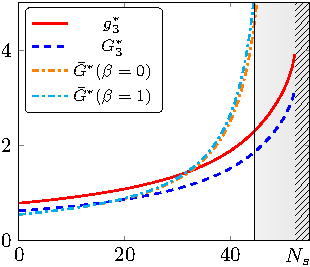
\includegraphics[width=\linewidth]{NS_findiff_all_hss_all_g-crop.pdf}
\caption{We show the fixed-point values for the three Newton couplings:
	The three-graviton coupling (red continuous line), the graviton-scalar-coupling (blue dashed line) and the background coupling (dot-dashed orange line).}
\label{fig:NewtoncouplingFPs}
\end{figure}
%

%
\begin{widetext}
\begin{figure*}
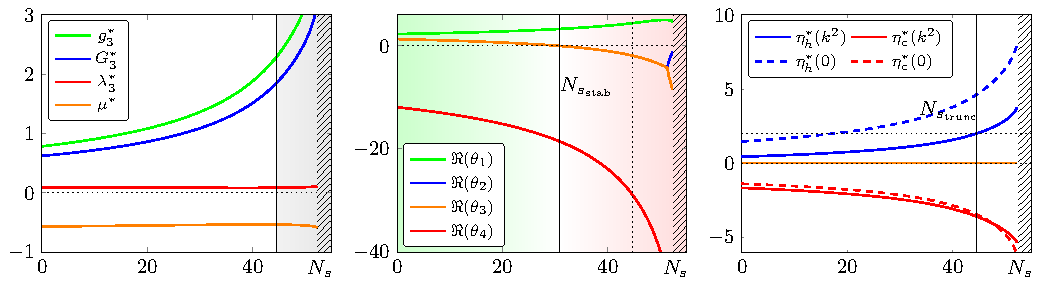
\includegraphics[width=\textwidth]{NS_findiff_all_hss_b.pdf}
\caption{We plot fixed-point values, critical exponents and anomalous dimensions as a function of $N_S$.
	The line at $N_S \approx 17$ shows where $\eta_h(0)$ exceeds two, and the line at $N_S \approx 45$ shows where $\eta_h(k^2)$ also exceeds 2.}
\label{fig:allFPvalues}
\end{figure*}
\end{widetext}
%

As the fluctuation Newton couplings enter the graviton anomalous dimension, $\eta_h$ increases as a function of $N_S$, cf.~\autoref{fig:allFPvalues}.
This implies that the bounds on $\eta_h$, discussed in \cite{Meibohm:2015twa}, are violated at large $N_S$.

%
\subsection{Effective gravitational coupling}
%
Metric fluctuations enter the diagrams with a propagator of the form $\frac{G_{(n,m)}}{1+\mu} = g_{\rm eff,\,1}$ and $\frac{G_{(n,m)}}{\left(1+\mu\right)^2}= g_{\rm eff, \, 2}$,
which we define as the two effective gravitational couplings.
The second is the effective coupling associated to a graviton propagator with an insertion of $\partial_t R_k$.
For the flow of matter vertices, it is immediately apparent that these are the only two combinations of $G_{(n,m)}$ and $\mu$ that can appear.
The case of pure-gravity flows features additional factors of $G_{(n,0)}$ at the vertices associated to the number of external gravitons.
Accordingly, the beta functions contain different powers of $1/(1+\mu)$ than powers of $G_3$.
However, each internal graviton line is associated to either of the two above effective couplings.
% On the other hand, the effect of metric fluctuations on matter couplings is encoded within the effective coupling $g_{\rm eff}$.
As $\mu$ stays approximately constant as $N_S$ increases, while $G_3$ increases, $g_{\rm eff,\,1/2}$ increase as well, cf.~\autoref{fig:effectiveG}.

%
\begin{figure}
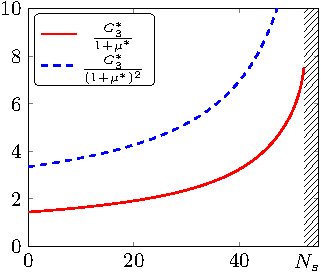
\includegraphics[width=\linewidth]{NS_findiff_all_hss_eff_g_only_ns-crop.pdf}
\caption{\label{fig:effectiveG} We plot the effective gravitational
  strength $G_3/(1+\mu)$ and $G_3/(1+\mu)^2$. The latter appears
  on propagators with the regulator insertion, whereas the former
  appears on propagators where the regulator insertion sits on another
  one of the internal legs of a diagram.}
\end{figure}
%
%
\subsection{Large $N_S$ limit}
%
In the limit of large $N_S$, all loops which are not given by closed
scalar loops, are suppressed by $\frac{1}{N_S}$. We assume that this
suppression is not counteracted by a scaling of couplings with $N_S$.
Accordingly, the results within our truncation simplify to the
following
%
\bea
\beta_{G_3} &=& 2 G_3 + 3 G_3 \eta_h - \sqrt{G_3}g_3^{3/2}N_S\, \frac{86}{1140 \pi},\\
\beta_{g_3}&=& 2 g_3 + g_3 \eta_h,\\
\eta_h &=& g_3 N_S \frac{1}{24 \pi},\\
\eta_S&=&0.  \eea
%
As the system is only driven by scalar fluctuations, the increase of
$\eta_h$ does not pose a problem for the choice of regulator.

This system admits three fixed points \bea
G_{3\, \ast}&=&0,\, g_{3\, \ast}= 0,\quad \theta_{1,2} =-2,\\
G_{3\, \ast}&=&-\frac{355008 \pi}{9025 N_S},\, g_{3\, \ast}= -\frac{48 \pi}{N_S},\quad \theta_{1,2} =2,\\
G_{3\, \ast}&=&0,\, g_{3\, \ast}= -\frac{48 \pi}{N_S},\quad
\theta_1=2, \theta_2 \rightarrow - i\, \infty .  \eea

Due to the presence of the Gau\ss{}ian fixed point, the fixed point at
negative $G_3, g_3$ cannot be connected to positive values of the
Newton coupling in the infrared.


\section{Nielsen identity \& applications}
Now we exploit the Nielsen identity (NI) or split Ward identity (sWI) to
improve upon the background field approximation. Related derivations
and application in the present context can be found in
\cite{Litim:2002ce,Litim:2002hj,Pawlowski:2003sk,PawlowskiH,Pawlowski:2005xe,Donkin,Donkin:2012ud}. In
general split Ward identitites have also been discussed in
% \cite
{Reuter-Wetterich1997,Reuter1998ff,Morrisetal2013ff,Safari2015
% }
{\coljmp please fill in}.

With the introduction of a background field,
the effective action becomes a functional of both
the dynamical fluctuation field $\Delta\Phi$ and the auxiliary
background field $\bar\Phi$
\begin{align}
\Gamma_k=\Gamma_k[\bar\Phi,\Delta\Phi].
\end{align}
In the present case of
gravity coupled to scalar matter the background and fluctuation fields read
\begin{align}
  \bar\Phi=(\bar g, 0,0,\bar \phi)\,,\qquad \Delta\Phi= (h,C,\bar
  C,\varphi)\,,
\end{align}
respectively,
where the full metric field is given by $g=\bar g+h$ and full scalar field
by $\phi=\bar\phi+\varphi$.

In scalar theories it is easily seen that for
vanishing cutoff $k=0$ the effective action is a functial of
the full field
$\phi=\bar\phi+\varphi$ only.
This is due to the fact that the classical action has
this property,
$S_{\text{\tiny cl}}[\bar\phi,\varphi]=S_{\text{\tiny
    cl}}[\bar\phi+\varphi]$.
The shift symmetry is then broken
by introducting the cutoff term $R_k=R_k[\bar\phi]$.
The resulting difference in the field dependencies is
then expressed by the NI or sWI as follows
\cite{Litim:2002hj}
\begin{align}\label{eq:scalarNIk}
	\0{\delta \Gamma_k}{\delta\bar\phi}-\0{\delta
	\Gamma_k}{\delta\varphi} =
	\012\, \Tr \left(
		G_k[\bar\phi,\varphi]\,
		\0{\delta R_k[\bar\phi]}{\delta \bar\phi}
	\right) \,,
\end{align}
for applications see e.g.\ \dots%\cite{Morrisetal}.
For flows towards the
infrared Eq. \eq{eq:scalarNIk} suggests
to use the background approximation
\begin{align}\label{eq:backapprox}
	\Gamma_k[\bar\phi,\varphi]\approx \Gamma_k[\bar\phi,\varphi=0]\,,
\end{align}
which is exact for $k=0$.
However, for flows towards the UV ($k\to\infty$)
the background approximation
is spoiled by powercounting leading
terms in the effective action,
even in asymptotically safe scalar theories.

In gauge theories the situation is even more complicated.
In this case
there are two sources for a genuine background dependence.
Besides the cutoff term which is present in scalar theories as well,
there is an additional source coming from the gauge fixing sector
$S_{\text{\tiny gauge}}=S_{\text{\tiny gf}}+S_{\text{\tiny ghost}}$.
Both the gauge fixing term $S_{\text{\tiny gf}}$ and the
ghost term $S_{\text{\tiny ghost}}$ have to depend on the background
gauge field if background gauge invariance is demanded.
This shows that the motivation for introducing the background field, namely
background gauge invariance, leads to a genuine background
dependence of the effective action.

In the present application to the gravity scalar system we
drop the background scalar, as we have a free scalar theory and only
deal with the background metric. Then the simple scalar NI of Eq.
\eq{eq:scalarNIk} turns into
\begin{align}\nonumber
	\0{\delta \Gamma_k}{\delta\bar g_{\mu\nu}}-\0{\delta
	\Gamma_k}{\delta h_{\mu\nu}} =& \012 \,\01{\sqrt{\bar g}} \Tr\, \0{\delta \sqrt{\bar g}
	R_k[\bar g]}{\delta \bar g_{\mu\nu}}\, G_k[\bar g, h]\\[2ex]
	&+\left\langle \0{\delta S_{\text{\tiny
	gauge}}[\bar g,h]}{\delta \bar g_{\mu\nu}}
	-\0{\delta S_{\text{\tiny gauge}}[\bar g,h]
}{\delta h_{\mu\nu}}\right\rangle \,,
\label{eq:gaugeNIk}\end{align}
where the second line originates from the genuine background field
dependendence of the gauge fixing sector and we have dropped the
dependence of the other fields. The regulator $R_k$ is a matrix in field
space,
\begin{align}
	R_k= \left( \begin{array}{cccc} R_h & 0 & 0 & 0\\
	0 &0& R_c&  0 \\
	0 &-R_c &0 &0 \\
0 & 0& 0& R_\varphi\end{array}\right)\,.
\end{align}
and the trace involves a symplectic metric in the ghost subsector. The
second line in \eq{eq:gaugeNIk} survives in the limit $k\to 0$. This
casts some doubt on the use of background field approximations even
for infrared flows.

{\colpl (I think the following paragraph is a bit
	repetitive in itself and should be shortend) [}
Indeed, in Yang-Mills theories in covariant gauges the fluctuation
propator shows the Yang-Mills mass gap that signals confinement while
the background propagator has no mass gap. Identifying the former with
the latter in the flow leads to a loss of confinement: within the
background field approximation the potential of the order parameter,
the Polyakov loop variable $\langle \tr \, \CP \exp \, i g_s
\int_0^{1/T} A_0 dt\rangle $, does not show the confining minimum
which is directly related to the mass gap in the gluon propagator in
covariant gauges. Whether or not all confining properties are lost is
difficult to access. However, at least in the standard vertex
expansion scheme this statement holds. This expansion scheme also
underlies most quantum gravity computations. Despite the fact that the
physics mechanisms working in infrared QCD are certainly qualitatively
different from that working in UV gravit....
{\colpl ]}

Let us now briefly illustrate the use of the NI
%\eq{eq:gaugeNIk}
in the case of
pure Yang-Mills theory in a covariant gauge (cf. in particular
\cite{PawlowskiH}, Chapter IV C, page 61ff) for the example of the
universal one-loop beta function.
Splitting the full field as
$A_\mu=\bar A_\mu+a_\mu$,
the covariant background gauge reads
\begin{align}
	\bar D_\mu a_\mu \equiv (\partial_\mu + i\,g\,\bar A_\mu) \, a_\mu=0\,.
\end{align}
{\colpl (I think this is never used and not actually relevant.)}
The beta function of the coupling can be read off from that of the
running of the $\tr \,\bar F^2$-term in the background effective
action $\Gamma_k[\bar A]=\Gamma_k[\bar A, a=0]$.
{\colpl (Maybe this needs some more explanation.)}
The beta function can then be derived from the flow as follows
\begin{align}\label{eq:betabarA}
	\dot \Gamma_k[\bar A]\Big|_{\tr \bar F^2} = - 2 \bar \beta_g
	S_{\text{\tiny YM}}[\bar A]\,,
\end{align}
which comes about due to background gauge invariance.
{\colpl (Again, maybe this needs some more explanation.)}
It turns out that regulators that scale in the infrared as
\begin{align}\label{eq:IRRk}
	p^2 \, r \left( \0{p^2}{k^2} \right)
	\sim k^2  \left( \0{k^2}{p^2} \right)^{n-1}\,,
\end{align}
{\colpl (I've simply rewritten the expression in momentum space.
I think the rhs should also have a $p^2$ instead of $k^2$)}
lead to a background beta function $\bar \beta_g = (1+n)
\beta_{g,\rm 1-loop}$ and are hence regulator-dependent. In turn the
beta function computed from the fluctuation diagrams is
regulator-independent, $\beta_g=\beta_{g,\rm 1-loop}$, which reflects
the one-loop universality of the Yang-Mills beta function.
This result is surprising as the beta function is a universal
quantity.

This puzzle can be resolved as follows. First we notice
that an evaluation of the fluctuation correlation functions reveals
the correct one-loop beta function. Secondly, in the background
field approximation the $\Tr\,\bar F^2$-term also receives
contributions from the background field dependence of the regulator.
This $\bar A$-dependence triggered by the regulator should not be seen
as a genuine field dependence. Indeed, for $k\to 0$ it disappears, cf. Eq.
\eq{eq:gaugeNIk}. This is why we have to disentangle the regulator field
depencence from the genuine one.
This can be done by writing the effective action as
\begin{align}
\label{eq:EAsplit}
\Gamma_k[\bar A,a] = \Gamma_{k,1}[a] + \Gamma_{k,2}[\bar A] + \Gamma_{k,3}[\bar A, a]\,,
\end{align}
where the second term originates from the $\bar A$-dependence of the regulator and
the last term accounts for gauge invariance under transformations of the full field.
We will see shortly that it vanishes in the present case.

To extract the regulator dependence, on simply takes a functional derivative of
the last expression with respect to the background field. The RG flow of
the resulting object can then be projected onto the relevant coupling
($\tr \, \bar F^2$ in the Yang-Mills case) to obtain the regulator contribution
of the beta function one is interested in. The physical beta function
is then given by the difference
\begin{align}
	\beta^{(\text{phys})} = \beta \, \big|_{a=0} - \bar \beta \,.
\end{align}

This is why we will investigate the flow of the background-dependence
of the effective action $\partial_t \delta_{\bar A} \Gamma_k$
\begin{align}
\label{eq:A-Rk}
	\partial_t \int_{y,z} \0{\delta R_k(y,z)}{\delta \bar A(x)}
	\0{\delta \Gamma_k}{\delta R_k(y,z)} =
	\012 \, \Tr\, \partial_t
	\left(\0{\delta R_k[\bar A]}{\delta \bar A(x)}\, G_k[\bar A,
	a]\right).
\end{align}
The right hand side of the equation can be rewritten as a sum of
traces depending on the spin-0 and spin-1 Laplacians, $\bar \Delta_0=
-\bar D^2$ and $\bar \Delta_1 =-\bar D^2\id -2 g \bar F$, respectively.
These traces can be expressed as
\begin{align}
	\label{eq:A-Rk1}
	\012 \,  \Tr\, \partial_t \left[\0{\delta R_k(\bar \Delta)}{\delta \bar
	A(x)}\, G_k(\bar \Delta )\right] =
  \frac{1}{2}
	\0{\delta }{\delta \bar A(x)}
	\Tr\, \partial_t F_{\text{\tiny RG}}(\bar\Delta)\,,
\end{align}
where
\begin{align}\label{eq:FA}
	\partial_t  F_{\text{\tiny RG}}(x)= \partial_t \int_{x_0}^x d x' \0{\partial
	R_k(x')}{\partial x'} G_k(x')\,.
\end{align}
{\colpl I would prefer another name that is less similar to the field strength tensor.
Also, one should mention that the fluctuation field dependence was already dropped.}
Note that the function $F_{\text{\tiny RG}}(x)$ is potentially
singular in the infrared, that is for $x\rightarrow 0$.  The infrared limit of
the regulators is given by \eq{eq:IRRk} and it follows that
\begin{align}\label{eq:IRF}
	F_{\text{\tiny RG}}(x\to 0)
	\propto x^{-(n-1)}\,,
\end{align}
where one has a logarithmic divergence for $n=1$. Accordingly, the
$t$-derivatives in \eq{eq:A-Rk}-\eq{eq:IRF} are required for
finiteness.

This shows how the NI \eq{eq:gaugeNIk} can trigger
contributions to logarithmically running quantitites already at
one-loop: IR-singular regulators introduce additional scales for
background observables.

Now we want to compute the contributions to $\tr\, \bar F^2$ that
come from the genuine background field dependence of the effective
action. This is done by removing the mixed contributions, $\tr\, \bar
F \bar F_{R_k}$, and $\tr \,\bar F_{R_k} \bar F_{R_k}$ contributions
from the full $\bar A$-dependence. Here, $F_{R_k}$ signals the field
strength of the regulator field. To that end we first notice that
mixed contributions to $\tr\, \bar F^2$ are not present: taking a
$\bar A$-derivative of \eq{eq:A-Rk1} that hits the genuine $\bar
A$-dependence leads to terms proportional to
\begin{align}
	\label{eq:mixed}
	- \partial_t
	\left[\Tr\,
		\int_{x_0}^x d x' \0{\partial
		R_k(x')}{\partial x'} G_k(x) \0{\delta
		\Gamma_k^{(2)}}{\delta\bar A} G_k
		\bigg|_{\tr \bar F^2}
	\right]=0\,.
\end{align}
Note that the occurance of $G_k^2$ leads to IR-finite expressions, and
hence the trace can be taken before taking the $t$-derivative. As we
concentrate on field-dependences with dimensionless coefficients, the
$t$-derivative vanishes (no other scale is present that could lead to
$\log k/{\rm scale}$ dependences).

This leaves us with the task to compute \eq{eq:A-Rk1}. The
right hand side is a trace of a functional of $\bar \Delta =
\bar\Delta_0, \,\bar\Delta_1$, and can be computed with standard
heat-kernel techniques. In case we are only interested in powers of $\Tr
\bar F^2$ the simplest way to compute the trace is by using
\begin{align}
	\label{eq:tau_expansion}
	\Tr f(\bar \Delta) =
	f(-\partial_\tau ) \Tr\, e^{-\tau \bar
	\Delta}\bigg|_{\tau=0} \,,
\end{align}
for a general function $f$, which avoids the standard Laplace
transform. In the present case of a Yang-Mills theory this straightforwardly
leads to
\begin{align}
	\label{eq:betabarARk}
  \frac{1}{2} \, \Tr\, \partial_t F_{\text{\tiny RG}}(\bar \Delta) \bigg|_{\tr \bar F^2}= -2 n
	\,\beta_{g,\rm 1-loop} S_{\text{\tiny YM}}[\bar A]\,.
\end{align}
Subtracting this result from \eq{eq:betabarA} leads us to
\begin{align} \label{eq:betabarAfinal}  \dot \Gamma_k[ \bar A]-
  \frac{1}{2} \, \Tr\, \partial_t F_{\text{\tiny RG}}(\bar \Delta)\bigg|_{\tr \bar
	F^2} = -2 \,\beta_{g,\rm 1-loop} S_{\text{\tiny YM}}[\bar A]\,,
\end{align}
which is indeed the regulator independent, universal beta function.

The above analysis in the Yang-Mills example suggests the following:
When using the background field approximation one should modify the
second derivative w.r.t.\ the background field in order to account
for the regulator dependence of the background field.

We work with the approximation
\begin{align}
	\lim_{k\to \infty} \left(\0{\delta \Gamma_k}{\delta\bar g_{\mu\nu}}-\0{\delta
		\Gamma_k}{\delta h_{\mu\nu}} \right)\simeq \012 \Tr\, \0{1}{ \sqrt{\bar g} } \0{\delta\sqrt{\bar g} R_k[\bar
	g]}{\delta \bar g_{\mu\nu}}\, G_k[\bar g, h]\,,
\label{eq:gravappNIk}\end{align}
where the have dropped the second line with the gauge fixing
contributions: they account for the difference of the wave function
renormalisation of the fluctuating graviton and the background
graviton propagator.

As opposed to infrared Yang-Mills theory we do
not expect qualitative differences in the UV. Still we remark that in
Yang-Mills theory the (genuine) background anomalous dimension
$\eta_{\bar A}=-\partial_t \log Z_{\bar A}=2 \beta_g$, and the
fluctuating anomalous dimension $\eta_{\bar a}=-\partial_t \log
Z_{\bar a}$ differ by approximately a factor two (in the Landau
gauge). Moreover, while the latter is gauge-dependent, the former is
not. This difference is at the heart of the background approximation,
and together with the missing confinement properties is a strong
incentive to use a full fluctuation approach.

However, here we only
want to improve on the regulator-induced part of the background field
approximation.
Note also that if one compares the contributions
of the cutoff term and the gauge fixing sector to the UV flow,
combinatorial arguments suggest that the cutoff term is of
dominant importance.
This is because it couples to all fluctuations modes
of the graviton, while the contributions of the gauge fixing sector
couple directly to the longitudinal modes only: the derivative of the gauge
fixing term is proportional to $h*F(\bar g) \delta F/\delta \bar g
h$.
% This suggests the dominance of the cutoff terms in the UV where
% the only scale is the cutoff scale.

Strictly speaking, however, this
argument only applies to renormalisation group invariant quantities
such as the Newton coupling $g_N$ with
\begin{align}
	\mu\0{d}{d\mu} g_N=0\,,
\end{align}
where $\mu$ is the renormalisation group scale of the underlying
theory. In summary, this leads us to a modified background field
approximation for the two-point function by taking the $h$-derivative
of \eq{eq:gravappNIk}.
Applying the operator $\delta_{\bar g} + \delta_h$ once more to
\eq{eq:gravappNIk} and dropping mixed derivatives then results in
\begin{align}
	\0{\delta^2 \Gamma_k}{\delta h_{\mu\nu}\delta h_{\rho\sigma}}&\simeq
	\0{\delta^2 \Gamma_k}{\delta \bar g_{\mu\nu}\delta \bar g_{\rho\sigma}}  \notag \\
	&-\012 \left(\0{\delta}{\delta\bar g_{\rho\sigma}}+\0{\delta}{\delta h_{\rho\sigma}}
		\right) \Tr\left[ \0{1}{\sqrt{\bar g}}\0{\delta \sqrt{\bar g} R_k[\bar g]}{\delta \bar g_{\mu\nu}}\, G_k[\bar
	g, h]\right]\,.
\label{eq:gravpropNIk}
\end{align}
We have shown at the example of Yang-Mills theory, that the
fluctuation field derivative of the term in the square brackets on the
right hand side of \eq{eq:gravpropNIk} gives sub-leading
contributions only.
In analogy we assume that the same feature holds in
gravity, and arrive at the final approximation for the fluctuating
two-point function
\begin{align} \label{eq:modback}
	\0{\delta^2 \Gamma_k}{\delta h_{\mu\nu}\delta h_{\rho\sigma}}&\approx \0{\delta^2 \Gamma_k}{\delta \bar g_{\mu\nu}\delta \bar g_{\rho\sigma}}
	- \0{\delta}{\delta \bar g_{\rho\sigma}} \int \0{1}{\sqrt{\bar g}}\0{\delta \sqrt{\bar g} R_k}{\delta \bar g_{\mu\nu}}\0{\delta
	\Gamma_k}{\delta R_k}\,,
\end{align}
This approximation has been used in gravity e.g.\ in
\cite{Donkin,Donkin:2012ud}. Apart from the standard background
two-point function it contains a second, purely regulator induced term.
The flow of this term is simply given by
\eq{eq:FA}, which we recall was given by
\begin{align}\label{eq:Fg}
	F_{\text{\tiny RG}}(x)= \int_{x_0}^x \mathrm dx' \; \0{\partial R_k(x')}{\partial x'} \, G_k(x')\,,
\end{align}
where we have restricted ourselves to IR-finite regulators.
As a reminder, these equations stem from
\begin{align}
 \partial_t \delta_{\bar g} \Gamma_k = \delta_{\bar g} \partial_t \Gamma_k \,,
\end{align}
which entails the equation
\begin{align} \label{eq:commuted-flow}
 \012 \partial_t \Tr \left[ \01{\sqrt{\bar g}} G_k \0{\delta  \sqrt{\bar g} R_k}{ \delta \bar g_{\mu\nu}}  \right]
 = \012 \0{\delta}{\delta \bar g_{\mu\nu}} \Tr \left[ G_k \partial_t R_k \right] \,,
\end{align}
see \cite{Litim:2002ce} same equation in the context of a Yang-Mills theory.
We further note that
\begin{align}
 \0{\delta}{\delta \bar g_{\mu\nu}} F_{\text{\tiny RG}}(\bar \Delta)
 &= \0{\delta}{\delta \bar g_{\mu\nu}} \int_{x_0}^{\bar\Delta} d x' \0{\partial R_k(x')}{\partial x'} G_k(x') \notag \\
 &= \0{\delta \bar \Delta}{ \delta \bar g_{\mu\nu}} \0{\partial R_k(\bar \Delta)}{\partial \bar \Delta} G_k(\bar \Delta) \notag \\
 &= \0{\delta R_k(\bar \Delta)}{ \delta \bar g_{\mu\nu}} G_k(\bar \Delta)\,,
\end{align}
is actually (almost) the left hand side of \eqref{eq:commuted-flow}.
Note further that $x_0$ dependence in $F_{\text{\tiny RG}}$ drops out in the end since we are taking a $\delta_{\bar g}$ deravative.


\Eq{eq:Fg} can straightforwardly be computed with heat-kernel methods.
Similarly to our Yang-Mills example we have for IR-finite regulators
\begin{align}\nonumber
  \012 \Tr\, \0{1}{\sqrt{\bar g}}\left[\0{\delta \sqrt{\bar g} \, R_k(\bar \Delta)}{\delta \bar g_{\mu\nu}(x)}\,
  G_k(\bar \Delta )\right] =&  \, \frac{1}{2} \, \Tr\, \0{\delta }{\delta \bar g_{\mu\nu}(x)} F_{\text{\tiny{RG}}}(\bar\Delta)\\[2ex]
                            & +
                              \Tr \, \0{1}{\sqrt{\bar g}}\0{\delta \sqrt{\bar g}}{\delta \bar g_{\mu\nu}}\, R_k G \,.
\label{eq:g-Rkg}
\end{align}
Moreover, in gravity the luxury of using a background field for gauge
invariance turns into the necessity of using a background metric in
the gauge fixing sector (if one insists on linear gauge fixing in the
fluctuation field $h$). For UV flows the cutoff contributions have
leading contributions to relevant operators such as the two-, three-,
and four-point functions. In terms of diffeomorphism invariant objects
this relates to the running of cosmological constant $\Lambda$,
curvature scalar $R$ and curvature scalar squared $R^2$, the presumably
minimal set of relevant operators in asymptotically safe quantum
gravity.

In \cite{Manrique:2010am} the so-called bi-metric approach to quantum
gravity was put forward aiming at a distinction of the fluctuating
part of the metric and the background metric. For computational
reasons the following approximation was considered,
\begin{align}
	\Gamma_k[\bar g,h]= \Gamma_{\text{EH},k}[g]+\bar \Gamma_{\text{EH},k}[\bar g]+M_k \int d^4 x \sqrt{g}
	\left(\0{\sqrt{\bar g}}{\sqrt{g}}\right)^n\,,
\end{align}
where $\Gamma_{\text{EH}},\bar \Gamma_{\text{EH}}$ is the
Einstein-Hilbert actions with cutoff-dependent parameters. In later
extended computations, \cite{Becker:2014qya}, the last term has been
dropped, $M_k=0$. Evidently, this approximation violates the approximated NI
\eq{eq:gravpropNIk} and only holds if
\begin{align}
	\0{\delta}{\delta h_{\rho\sigma}} \Tr\left[\01{\sqrt{\bar g}}\0{\delta \sqrt{\bar g} R_k[\bar g]}{\delta \bar
	g_{\mu\nu}}\, G_k[\bar g, h]\right]\approx 0\,,
\end{align}
at least at $h=0$.

\subsection{Calculation Gravity}

We specialize the background to a sphere in four dimensions.
We are interested in evaluating the quantity
\begin{align}
  \nonumber
  I \equiv&\, \frac 12 \, \Tr
  \left[
    \frac{1}{\sqrt{\bar g}} \, G_k(\bar \Delta) \, \frac{\delta}{\delta \bar g_{\mu\nu}} \Big( \sqrt{\bar g} \, R_k(\bar\Delta) \Big)
  \right]\\%[2ex]
  =&\,
  \frac 14 \, \bar g^{\mu\nu} \, \Tr \Big[ G_k R_k - F_{\text{\tiny RG}}  \Big]
  + \frac{1}{2} \, \frac{\delta}{\delta \bar g_{\mu\nu}} \Big( \Tr \, F_{\text{\tiny RG}} \Big)% \\[2ex]
  \,,
  \label{eq:def-I}
\end{align}
where $F_{\text{\tiny RG}}(\bar \Delta)$ is the functional introduced in equation (\ref{eq:FA}).

Here it seems that the $x_0$ dependence of $F_{\text{\tiny RG}}$ does not drop out anymore,
since $\Tr F_{\text{\tiny RG}}$ appears without a $\delta_{\bar g}$ derivative.
This is, however, a false conclusion since only in $\Tr \delta_{\bar g} F_{\text{\tiny RG}}$ the $x_0$ part vanishes
while in $\delta_{\bar g} \Tr F_{\text{\tiny RG}}$ the derivative hits the $\sqrt{\bar g}$ part of the trace
and the $x_0$ part of this term precisely cancels the $x_0$ part of $\Tr F_{\text{\tiny RG}}$ without a $\delta_{\bar g}$ derivative.
On the other hand the zero point function is given by
\begin{align}
  \frac 12 \, \Tr \Big[ G_k(\bar \Delta) \dot R_k(\bar \Delta) \Big] \,.
  \label{eq:background_flow}
\end{align}
where it is particular interesting to look for sign changes compared to the flow of the one point function.
% The latter is given in our approximation by
% \begin{align}
%  \Delta \equiv  \frac 12 \frac{\delta}{\delta \bar g_{\mu\nu}} \Tr \Big[ G_k(\bar \Delta) \dot R_k(\bar \Delta) \Big] - \partial_t I \,.
% \end{align}

All traces appearing in the above expressions can be evaluated using heat kernel techniques.
Details of the computation and intermediate results can be found in appendix \ref{app:traces}.

The results for $I$ and the flow (\ref{eq:background_flow}) in the gravity sector are
given by
\begin{align}
  \notag
  I =& \, \frac{ \sqrt{\bar g} \, \bar g^{\mu\nu} }{ 32 \pi^2 } \,
  \bigg\lbrace
    \bigg[
    \frac 5{12} \frac{1}{1 - 2 \lambda}
    + \frac 1{12} \frac{1}{1 - \frac 43 \lambda}
    - \frac{1}{3}
    \bigg] k^4 \\ \notag
    + &\bigg[
        \frac {5}{18} \frac{1}{(1 - 2 \lambda)^2}
      + \frac {13}{144}
    \bigg] k^2 \bar R \\ \notag
    + &\bigg[
      - \frac {5}{9} \frac{1}{(1 - 2 \lambda)^3}
      - \frac {5}{36} \frac{1}{(1 - 2 \lambda)^2}
      + \frac {1}{864} \frac{1}{1 - 2 \lambda} \\
      &- \frac {29}{4320} \frac{1}{1 - \frac 43 \lambda}
      - \frac {61}{1440}
    \bigg] \bar R^2
  \bigg\rbrace
    + \mathcal O (\bar R^3) \,,
\end{align}
\begin{align}
  &\frac 12 \, \Tr \, G_k \dot R_k = \, \frac{ \sqrt \bar g }{ 32 \pi^2 }
  \bigg\lbrace
    \bigg[
      \frac{5 - \frac{5}{6} \eta_h}{1 - 2 \lambda}
      + \frac{1 - \frac{1}{6} \eta_h}{1 - \frac 43 \lambda} \notag \\
      & \quad - 4
      - \frac{2}{3} \, \eta_h
      + \frac{4}{3} \, \eta_c
    \bigg] k^4 \notag \\
    &+ \bigg[
      - \frac{10}{3} \frac{1 - \frac{1}{6} \eta_h}{(1 - 2 \lambda)^2}
      - \frac{5}{3} \frac{1 - \frac{1}{4} \eta_h}{1 - 2 \lambda}
      + \frac{1}{3} \frac{1 - \frac{1}{4} \eta_h}{1 - \frac 43 \lambda} \notag \\
      & \quad - \frac{23}{12}
      - \frac{7}{18} \, \eta_h
      + \frac{14}{18} \, \eta_c
    \bigg] k^2 \bar R \notag \\
    &+ \bigg[
        \frac{20}{9} \frac{1}{(1 - 2 \lambda)^3}
      + \frac{10}{9} \frac{1}{(1 - 2 \lambda)^2}
      - \frac{1}{216} \frac{1}{1 - 2 \lambda} \notag \\
      & \quad + \frac{29}{1080} \frac{1}{1 - \frac 43 \lambda}
      - \frac{149}{270}
    \bigg] \bar R^2
  \bigg\rbrace
    + \mathcal O (\bar R^3) \,.
\end{align}
For scalar fields we get the following contributions:
\begin{align}
  I^s
  & = \frac {\sqrt{\bar g} \, \bar g^{\mu\nu}}{32 \pi^2}
  \bigg[
      \frac{1}{12} \, k^4
    - \frac{29}{4320} \, \bar R^2
  \bigg]
  + \mathcal O (\bar R^3) \,,
  \\
  \frac 12 \, \Tr \, G_k^s \dot R_k^s
  & = \frac {\sqrt{\bar g}}{32 \pi^2}
  \bigg[
  k^4
  + \frac {1}{3} \, k^2 \, \bar R
  + \frac {29}{1080} \, \bar R^2
  \bigg]
  + \mathcal O (\bar R^3) \,.
  % \\
  % \Delta^s
  % & = \frac {\sqrt{\bar g} \, \bar g^{\mu\nu}}{32 \pi^2}
  % \bigg[
  %  \frac 16 \, k^4
  % + \frac 13 \, k^2 \, \bar R
  % + \frac {29}{720} \, \bar R^2
  % \bigg]
  % + \mathcal O (\bar R^3)
\end{align}



\begin{figure*}
\includegraphics[width=0.49\textwidth]{Background-g-comparison}
\hfill
\includegraphics[width=0.49\textwidth]{Fluctuation-g-comparison}
\caption{Comparison of different gravitational couplings.
In the left panel the background gravitational coupling is plotted with different input on the right hand side.
In the right panel the highest dynamical coupling of different systems is plotted.
The first system is the pure background system, the second is the level one improved background system and the last one is the fully fluctuating system.}
\label{fig:Comparison-of-g}
\end{figure*}

\begin{figure*}
\includegraphics[width=0.49\textwidth]{Background-lam-comparison}
\hfill
\includegraphics[width=0.49\textwidth]{Fluctuation-lam-comparison}
\caption{Comparison of different $\lambda$ couplings.
In the left panel the background cosmological constant coupling is plotted with different input on the right hand side.
In the right panel the highest dynamical $\lambda$ coupling of different systems is plotted.
The first system is the pure background system, the second is the level one improved background system and the last one is the fully fluctuating system.
In the right panel all couplings are bound by the value $\012$, while in the left panel only $\bar \Lambda*(\eta_N,\bar\Lambda^*)$ is bound by that value.}
\label{fig:Comparison-of-lam}
\end{figure*}

\begin{figure*}
\includegraphics[width=0.49\textwidth]{All-g-from-fluc}
\hfill
\includegraphics[width=0.49\textwidth]{All-lam-from-fluc}
\caption{
Comparison of different level-$n$ gravitational couplings (left) and 'cosmological constants' (right).
All couplings were evaluated with the input of the full fluctuation system on the right hand side.
While the gravitational couplings behave qualitatively similar, the level-$n$ 'cosmological constants' display significant differences in their behaviour.
This emphasises again the necessaty to treat the graviton mass parameter in a fluctuation computation.
}
\label{fig:All-from-fluc}
\end{figure*}

\begin{figure*}
\includegraphics[width=0.49\textwidth]{All-g-from-mu}
\hfill
\includegraphics[width=0.49\textwidth]{All-lam-from-mu}
\caption{Comparison of different level-$n$ gravitational couplings (left) and 'cosmological constants' (right).
Here we combined the flow equation for the graviton mass parameter $\mu$ with different flow equations for the Newton's coupling.
All couplings behave qualitatively similar and thus we conclude that the correct treatment of the graviton mass parameter is essential for qualitatively reliable results.}
\label{fig:All-from-mu}
\end{figure*}


\subsection{Flow equations for background and level one couplings}

We have made the approximation
\begin{align}
 \0{\delta}{\delta h_{\mu\nu}} \Gamma_k \approx  \0{\delta}{\delta {\bar g}_{\mu\nu}} \Gamma_k  - \012 \Tr \01{\sqrt{\bar g}} \0{\delta \sqrt{\bar g} R_k }{ \delta {\bar g}_{\mu\nu} } G_k\,,
\end{align}
and consequently
\begin{align}
 \0{\delta}{\delta h_{\mu\nu}} \partial_t \Gamma_k \approx  \0{\delta}{\delta {\bar g}_{\mu\nu}} \partial_t \Gamma_k  - \partial_t I
 % = \Delta
 \,.
\end{align}
For the pure background couplings we obtain
\begin{align}
 \partial_t \bar G &= (2 + \eta_N) \bar G \\
 \partial_t \bar \Lambda &= - 4 \bar \Lambda + \0{\bar \Lambda}{\bar G} \partial_t \bar G + 8 \pi \bar G I_3\bigg|_{\bar R = 0} \\
 \eta_N &= 16 \pi \bar G I_3\bigg|_{\bar R \text{ lin}}
\end{align}
with
\begin{widetext}
\begin{align}
I_3\bigg|_{\bar R = 0}&=  \frac{ \sqrt \bar g }{32\pi^2}\left(5\0{1-\0{\eta_h}{6}}{1-2\lambda}+4(1-\0{\eta_h}{6})+\0{1-\0{\eta_h}{6}}{1-\043 \lambda}-8(1-\0{\eta_c}{6})+N_s\right)\\
  I_3\bigg|_{\bar R \text{ lin}} &= \frac{ \sqrt \bar g }{32\pi^2} \left(-\0{10}3  \0{1-\0{\eta_h}6}{(1-2\lambda)^2} - \053 \0{1-\0{\eta_h}4}{1-2\lambda} + \054 \left(1-\0{\eta_h}5\right) + \013 \0{1 - \0{\eta_h}4}{1-\043 \lambda} + \023 \left( 1 - \0{5\eta_h}{24}\right) - \0{23}6 \left(1 - \0{14\eta_c}{69}\right)+\0{N_s}3\right)
\end{align}
\end{widetext}

The flow equations for the level one couplings can be expressed by the previous quantities plus some improvement
\begin{align}
 \partial_t \bar G_1 &= (2 + \eta_{N,1}) \bar G_1 \\
 \partial_t \bar \Lambda_1 &= - 4 \bar \Lambda_1 + \0{\bar \Lambda_1}{\bar G_1} \partial_t \bar G_1 + 8 \pi \bar G_1 \left(  I_3 - 8 I \right) \bigg|_{\bar R = 0} \\
 \eta_{N,1} &= 16 \pi \bar G_1 \left( I_3 - 2 I  \right)\bigg|_{\bar R \text{ lin}}
\end{align}
with
\begin{align}
  I\bigg|_{\bar R = 0}&=  \frac{ \sqrt \bar g }{32\pi^2}\left(\05{12} \0{1}{1-2\lambda}+\01{12}\0{1}{1-\043 \lambda}-\013+\01{12} N_s\right)\\
  I\bigg|_{\bar R \text{ lin}} &= \frac{ \sqrt \bar g }{32\pi^2} \left(\05{18}\0{1}{(1-2\lambda)^2} + \0{13}{144} \right)
\end{align}

\section{Comparison of different flow equations}

These are the flow equations with all anomalous dimensions set to zero and with $\bar\lambda=\lambda_n=0$ and $\eta_\phi=0$ on the right hand side
\begin{align}
 \partial_t \bar g &\sim -\frac{27}{8 \pi} {\bar g}^2 + \frac1{6\pi}{\bar g}^2 N_s \notag\\
  &\approx -1.1 {\bar g}^2 + 0.053 {\bar g}^2 N_s \,, \label{eq:barg-simple}\\
 \partial_t (-Z_h) &\sim  \frac{19}{12 \pi}g + \01{24 \pi} g N_s \notag\\
  &\approx 0.5 g + 0.013 g N_s \,,\label{eq:etah-simple}\\
 \partial_t g &\sim -\frac{833}{285 \pi }g^2 -\0{43}{570 \pi} g^2 N_s\notag\\
  &\approx -0.93 g^2 - 0.024 g^2 N_s \,,\label{eq:g3-simple}\\
 \partial_t \bar \lambda &\sim \01{2\pi} \bar g + \frac1{4\pi}{\bar g}N_s \notag\\
  &\approx  0.16 \bar g + 0.08 \bar g N_s \,,\label{eq:barlam-simple}\\
 \partial_t (-\0{\mu}2) &\sim \frac{17}{12 \pi }g - \01{24 \pi} g N_s \notag\\
  &\approx 0.45 g - 0.013 g N_s \,,\label{eq:mu-simple}\\
 \partial_t \lambda_3 &\sim \frac{33}{20 \pi }g - \01{60 \pi}g N_s\notag\\
  &\approx 0.53 g - 0.0053 g N_s \,.\label{eq:lam3-simple}
\end{align}



\section{Conclusions}

The flow equation for the graviton mass parameter is the most important one.

\section{Evaluation of traces} \label{app:traces}

In this appendix we want to give a more detailed outline on how to
calculate the trace expression
\begin{align}\nonumber
 I \equiv&\, \frac 12 \, \Tr
  \left[
    \frac{1}{\sqrt{\bar g}} \, G_k(\bar \Delta) \, \frac{\delta}{\delta \bar g_{\mu\nu}} \Big( \sqrt{\bar g} \, R_k(\bar\Delta) \Big)
  \right]\\[2ex] \nonumber
=&\,
\frac 14 \, \bar g^{\mu\nu} \, \Tr \, G_k R_k + \frac 12 \, \Tr \, \frac{\delta}{\delta \bar g_{\mu\nu}} \, F_{\text{\tiny RG}}\\[2ex] \nonumber
=&\,
\frac 14 \, \bar g^{\mu\nu} \, \Tr \, G_k R_k
+ \frac 12 \, \frac{\delta}{\delta \bar g_{\mu\nu}} \, \Tr \, F_{\text{\tiny RG}} \\ \notag
&- \frac 12 \, \Tr \, \bigg[ \frac{1}{\sqrt{\bar g}} \left( \frac{\delta}{\delta \bar g_{\mu\nu}} \sqrt{\bar g} \right) F_{\text{\tiny RG}} \bigg] \\[2ex] \notag
=&\,
\frac 14 \, \bar g^{\mu\nu} \, \Tr \, \Big( G_k R_k - F_{\text{\tiny RG}} \Big)
+ \frac 12 \, \frac{\delta}{\delta \bar g_{\mu\nu}} \, \Tr \, F_{\text{\tiny RG}} \\[2ex]
=&\,
\frac 12 \, \bar g^{\mu\nu} \, \Big( I_1 - I_2 \Big) + \frac{\delta}{\delta \bar g_{\mu\nu}} \, I_2 \,.
\end{align}
For ease of notation we introduced
\begin{align}
  I_1 &\equiv \frac 12 \, \Tr \, G_k R_k \,, \\
  I_2 &\equiv \frac 12 \, \Tr \, F_{\text{\tiny RG}} \,.
\end{align}
For later convenience we will also abbreviate the background flow by
\begin{align}
  I_3 &\equiv \frac 12 \, \Tr \, G_k \dot R_k \,.
\end{align}
Following \cite{Codello:2008vh}, we may write
\begin{align}
  I_1 =& \,
  \frac{1}{32 \pi^2}
  \Big[ B_0(\bar\Delta) Q_2(R_kG_k)
    + B_2(\bar\Delta) Q_1(R_kG_k) \notag \\
  & + B_4(\bar\Delta) Q_0(R_kG_k)
  \Big]
  + \mathcal O (R^3) \,,
\end{align}
where
\begin{align}
  Q_n[W] &= \frac 1{\Gamma(n)} \, \int \mathrm dx \; x^{n-1} \, W(x) \,, \\
  B_n &= \int \mathrm d^dx \, \sqrt{\bar g} \; \tr \, b_n \,,
\end{align}
and $\tr \, b_n(\bar\Delta_s) \propto R^{n/2}$ are the  heat kernel coefficients.
We are interested in the function
\begin{align}
  W(x) = \frac{r_k(x)}{[x+r_k(x)+a \, \lambda \, k^2]^b} \,,
\end{align}
with constants $a$ and $b$, and dimensionless cosmological constant $\lambda$.
Using the optimized cutoff function
\begin{align}
  r_k(x) = (k^2-x) \, \theta( k^2-x) \,,
\end{align}
one finds
\begin{align}
  Q_2 &= \frac 16 \frac {k^4}{(1 + a \lambda)^b} \,, \\
  Q_1 &= \frac 12 \frac {k^2}{(1 + a \lambda)^b} \,, \\
  Q_0 &= \frac {k^0}{(1 + a \lambda)^b} \,.
\end{align}
In the limit $\beta \rightarrow \alpha$, $\alpha \rightarrow 0$,
the trace of $R_k G_k$ can be evaluated following the procedure in
\cite{Gies:2015tca} and is given by the sum of the contributions
of the four modes $h^{TT}_{\mu\nu}, \xi^{\mu}, h$ and $\sigma$. They are given
(in that order) for $\eta_h=0=\eta_c$ by
\begin{align}
  & \frac{r_k(x)}{x+r_k(x) - 2 \, \lambda \, k^2} - \frac 23 \, \bar R \, \frac{r_k(x)}{(x+r_k(x) - 2 \, \lambda \, k^2) ^2} \notag \\
    &\hspace*{0.7cm} + \frac 49 \, \bar R^2 \, \frac{r_k(x)}{(x+r_k(x) - 2 \, \lambda \, k^2) ^3} \\
  & \frac{r_k(x)}{x+r_k(x)} + \frac 14 \, \bar R \, \frac{r_k(x)}{(x+r_k(x)) ^2} + \frac{1}{16} \, \bar R^2 \, \frac{r_k(x)}{(x+r_k(x)) ^3} \\
  & \frac{r_k(x)}{x+r_k(x) - \frac 43 \, \lambda \, k^2} \\
  & \frac{r_k(x)}{x+r_k(x)} + \frac 13 \, \bar R \, \frac{r_k(x)}{(x+r_k(x)) ^2} + \frac{1}{9} \, \bar R^2 \, \frac{r_k(x)}{(x+r_k(x)) ^3}
\end{align}
The vector and scalar ghost contributions are given by
\begin{align}
  & - 2 \frac{r_k(x)}{x+r_k(x)} - \frac 12 \, \bar R \, \frac{r_k(x)}{(x+r_k(x)) ^2} - \frac{1}{8} \, \bar R^2 \, \frac{r_k(x)}{(x+r_k(x)) ^3} \,, \\
  & - 2 \frac{r_k(x)}{x+r_k(x)} - \frac 23 \, \bar R \, \frac{r_k(x)}{(x+r_k(x)) ^2} - \frac{2}{9} \, \bar R^2 \, \frac{r_k(x)}{(x+r_k(x)) ^3} \,.
\end{align}
Furthermore, on the sphere we have
\begin{align}
  B_0(\bar\Delta_s) &= \sqrt{ \bar g } \;\tr \, b_0 \,, \\
  B_2(\bar\Delta_s) &= \sqrt{ \bar g } \;\tr \, b_2 \,, \\
  B_4(\bar\Delta_s) &= \sqrt{ \bar g } \;\tr \, b_4 \,,
\end{align}
where the trace coefficients are given in \autoref{tab:coeff}.
\begin{table}
	\begin{center}
		\begin{tabular}{  c  c  c  c  }
			\toprule
			        & TTT & VT & S \\
			\midrule
      $\tr \, b_0$ & 5 & 3 & 1 \\
      $\tr \, b_2$ & $-\frac 56 R$  & $\frac 14 R$  & $\frac 16 R$  \\
      $\tr \, b_4$ & $-\frac {1}{432} R^2$  & $-\frac {7}{1440} R^2$  & $\frac {29}{2160} R^2$  \\
			\bottomrule
		\end{tabular}
	\end{center}
  \caption{Heat kernel coefficients for transverse traceless tensors (TTT), transverse vectors (VT)
  and scalars (S) on $S^4$.}
	\label{tab:coeff}
\end{table}

By specializing the coefficients $a$ and $b$ in the general expression above and evaluating the sum over
all spin modes, we find
\begin{align}
  &I_1 = \,  \frac{ \sqrt \bar g }{ 32 \pi^2 }
  \bigg\lbrace
    \bigg[
    \frac 56 \frac{1}{1 - 2 \lambda}
    + \frac 16 \frac{1}{1 - \frac 43 \lambda}
    - \frac 23
    \bigg] k^4 \bar R^0 \notag \\
    &+ \bigg[
      - \frac {5}{9} \frac{1}{(1 - 2 \lambda)^2}
      - \frac {5}{12} \frac{1}{1 - 2 \lambda}
      + \frac {1}{12} \frac{1}{1 - \frac 43 \lambda}
      - \frac {7}{18}
    \bigg] k^2 \bar R^1 \notag \\
    &+ \bigg[
      \frac {10}{27} \frac{1}{(1 - 2 \lambda)^3}
      + \frac {5}{18} \frac{1}{(1 - 2 \lambda)^2}
      - \frac {1}{432} \frac{1}{1 - 2 \lambda} \notag  \\
      & \quad + \frac {29}{2160} \frac{1}{1 - \frac 43 \lambda}
      - \frac {169}{1440}
    \bigg] k^0 \bar R^2
  \bigg\rbrace
    + \mathcal O (\bar R^3) \,.
\end{align}

In similar fashion, one can calculates
\begin{align}
  I_2 =& \, \frac{1}{32\pi^2} \, F_\text{\tiny RG}(-\partial_\tau)
  \Big[
    B_0(\bar\Delta_s) \, \tau^{-2} +
    B_2(\bar\Delta_s) \, \tau^{-1} \notag \\
    &+ B_4(\bar\Delta_s) \, \tau^{0}
  \Big] \bigg|_{\tau=0}
    + \mathcal O(R^3)
\end{align}
where we used \eq{eq:tau_expansion}. In particular, by utilizing the
identities
\begin{align}
  \frac 1{\tau^2} &= \int_0^\infty \mathrm dx \; x \, e^{-\tau x} \bigg|_{\tau=0} \\
  \frac 1\tau &= \int_0^\infty \mathrm dx \; e^{-\tau x} \bigg|_{\tau=0}
\end{align}
one can evaluate the action of the differential operators, and we find
\begin{align}
  F_\text{\tiny RG}(-\partial_\tau) \tau^{-2} &= \int_0^\infty \mathrm dx \; x \, F_\text{\tiny RG}(x) \notag \\
  &= - \frac 13 \frac{k^4}{(1+a\lambda)^b} + x_0\text{-terms} \\
  F_\text{\tiny RG}(-\partial_\tau) \tau^{-1} &= \int_0^\infty \mathrm dx \; F_\text{\tiny RG}(x) \notag \\
  &= - \frac 12 \frac{k^2}{(1+a\lambda)^b} + x_0\text{-terms} \\
  F_\text{\tiny RG}(-\partial_\tau) \tau^0    &= F_\text{\tiny RG}(0) \notag \\
  &= - \frac{k^0}{(1+a\lambda)^b} + x_0\text{-terms}
\end{align}
where the last equalities hold for the general function
\begin{align}
  F_\text{\tiny RG}(x) = \int^{x}_{x_0} \mathrm dy \; \frac{r'_k(y)}{(y+r_k(y)+a \, \lambda \, k^2)^b} \,,
\end{align}
using the optimized cutoff as before.

Specializing the coefficients $a$ and $b$ for the various spin modes and summing the contributions
we get
\begin{align}
  &I_2 = \, \frac{ \sqrt \bar g }{ 32 \pi^2 }
  \bigg\lbrace
    \bigg[
    - \frac 53 \frac {1}{1 - 2 \lambda}
    - \frac 13 \frac {1}{1 - \frac 43 \lambda}
    + \frac 43
    \bigg] k^4 \bar R^0 \notag \\
    &+ \bigg[
        \frac {10}{9} \frac{1}{(1 - 2 \lambda)^2}
      + \frac {5}{12} \frac{1}{1 - 2 \lambda}
      - \frac {1}{12} \frac{1}{1 - \frac 43 \lambda}
      + \frac {41}{72}
    \bigg] k^2 \bar R^1 \notag  \\
    &+ \bigg[
      - \frac {20}{27} \frac{1}{(1 - 2 \lambda)^3}
      - \frac {5}{18} \frac{1}{(1 - 2 \lambda)^2}
      + \frac {1}{432} \frac{1}{1 - 2 \lambda} \notag  \\
      & \quad - \frac {29}{2160} \frac{1}{1 - \frac 43 \lambda}
      + \frac {3}{20}
    \bigg] k^0 \bar R^2
  \bigg\rbrace
    + \mathcal O (\bar R^3) \,.
\end{align}

Finally, the right-hand side of the flow equation $I_3$ can be evaluated
in the same way as $I_1$, where the Heat Kernel Functionals now depend on
\begin{align}
  \tilde W(x) = \frac{\dot r_k(x)}{[x+r_k(x)+a \, \lambda \, k^2]^b} \,.
\end{align}
Using $\dot r_k(x) = 2 \, k^2 \, \theta(k^2-x)$ for the optimized cutoff, we find
\begin{align}
  Q_2[\tilde W] &= \frac {k^4}{(1 + a \lambda)^b} \,, \\
  Q_1[\tilde W] &= \frac {2 \, k^2}{(1 + a \lambda)^b} \,, \\
  Q_0[\tilde W] &= \frac {2 \, k^0}{(1 + a \lambda)^b} \,.
\end{align}
With these relations, we find
\begin{align}
  &I_3 = \, \frac{ \sqrt \bar g }{ 32 \pi^2 }
  \bigg\lbrace
    \bigg[
      \frac{5 - \frac{5}{6} \eta_h}{1 - 2 \lambda}
      + \frac{1 - \frac{1}{6} \eta_h}{1 - \frac 43 \lambda} \notag \\
      & \quad - 4
      - \frac{2}{3} \, \eta_h
      + \frac{4}{3} \, \eta_c
    \bigg] k^4 \bar R^0 \notag \\
    &+ \bigg[
      - \frac{10}{3} \frac{1 - \frac{1}{6} \eta_h}{(1 - 2 \lambda)^2}
      - \frac{5}{3} \frac{1 - \frac{1}{4} \eta_h}{1 - 2 \lambda}
      + \frac{1}{3} \frac{1 - \frac{1}{4} \eta_h}{1 - \frac 43 \lambda} \notag \\
      & \quad - \frac{23}{12}
      - \frac{7}{18} \, \eta_h
      + \frac{14}{18} \, \eta_c
    \bigg] k^2 \bar R^1 \notag \\
    &+ \bigg[
        \frac{20}{9} \frac{1}{(1 - 2 \lambda)^3}
      + \frac{10}{9} \frac{1}{(1 - 2 \lambda)^2}
      - \frac{1}{216} \frac{1}{1 - 2 \lambda} \notag \\
      & \quad + \frac{29}{1080} \frac{1}{1 - \frac 43 \lambda}
      - \frac{149}{270}
    \bigg] k^0 \bar R^2
  \bigg\rbrace
    + \mathcal O (\bar R^3) \,.
\end{align}

We now want to evaluate $I$, and in particular the first derivative
with respect to the background field.
Since $S^4$ is an Einstein manifold, and in particular
\begin{align}
  \bar R_{\mu\nu} = (d-1) \, \bar g_{\mu\nu} \,,
\end{align}
taking the trace implies $\bar R = d \, (d-1)$. This gives
\begin{align}
  \frac{\delta \bar R}{\delta \bar g_{\mu\nu}} = \frac 2d \, \bar R \, \bar g^{\mu\nu} \,.
\end{align}
In $d=4$ this implies
\begin{align}
  \frac{\delta \bar R^0}{\delta \bar g_{\mu\nu}} = 0, \quad \quad
  \frac{\delta \bar R^1}{\delta \bar g_{\mu\nu}} = \frac 12 \bar g^{\mu\nu} \bar R, \quad \quad
  \frac{\delta \bar R^2}{\delta \bar g_{\mu\nu}} = \bar g^{\mu\nu} \bar R^2 \,.
\end{align}
Using these relations, we can finally evaluate $I$ to be
\begin{align}
  \notag
  I =& \, \frac{ \sqrt{\bar g} \, \bar g^{\mu\nu} }{ 32 \pi^2 } \,
  \bigg\lbrace
    \bigg[
    \frac 5{12} \frac{1}{1 - 2 \lambda}
    + \frac 1{12} \frac{1}{1 - \frac 43 \lambda}
    - \frac{1}{3}
    \bigg] k^4 \bar R^0 \\ \notag
    + &\bigg[
        \frac {5}{18} \frac{1}{(1 - 2 \lambda)^2}
      + \frac {13}{144}
    \bigg] k^2 \bar R^1 \\ \notag
    + &\bigg[
      - \frac {5}{9} \frac{1}{(1 - 2 \lambda)^3}
      - \frac {5}{36} \frac{1}{(1 - 2 \lambda)^2}
      + \frac {1}{864} \frac{1}{1 - 2 \lambda} \\
      &- \frac {29}{4320} \frac{1}{1 - \frac 43 \lambda}
      - \frac {61}{1440}
    \bigg] k^0 \bar R^2
  \bigg\rbrace
    + \mathcal O (\bar R^3) \,.
\end{align}

For a pure scalar field we find the following results:
\begin{align}
  I_1^s
  & = \frac{ \sqrt \bar g }{ 32 \pi^2 }
  \bigg[
      \frac{1}{6} \, k^4
    + \frac{1}{12} \, k^2 \, \bar R
    + \frac{29}{2160} \, \bar R^2
  \bigg]
  + \mathcal O (\bar R^3) \,, \\
  I_2^s
  & = \frac{ \sqrt \bar g }{ 32 \pi^2 }
  \bigg[
    - \frac{1}{3} \, k^4
    - \frac{1}{12} \, k^2 \, \bar R
    - \frac{29}{2160} \, \bar R^2
  \bigg]
  + \mathcal O (\bar R^3) \,, \\
  I_3^s
  & = \frac{ \sqrt \bar g }{ 32 \pi^2 }
  \bigg[
  k^4
  + \frac{1}{3} \, k^2 \, \bar R
  + \frac{29}{1080} \, \bar R^2
  \bigg]
  + \mathcal O (\bar R^3) \,.
\end{align}

This implies
\begin{align}
  I^s &= \frac{ \sqrt{\bar g} \, \bar g^{\mu\nu} }{ 32 \pi^2 }
  \bigg[
    \frac{1}{12} \, k^4  - \frac{29}{4320} \, \bar R^2
  \bigg]
  + \mathcal O (\bar R^3) \,.
\end{align}


%----------------------------------------------------------------------------------------
%	Conclusions
%----------------------------------------------------------------------------------------

\chapter*{Conclusions and Outlook}
\addcontentsline{toc}{chapter}{Conclusions and Outlook}

In this thesis, blah, blah, blah.

%----------------------------------------------------------------------------------------
%	BIBLIOGRAPHY
%----------------------------------------------------------------------------------------

\nocite{*}
\bibliography{allrefs}
\bibliographystyle{unsrt}
\addcontentsline{toc}{chapter}{\textcolor{ocre}{Bibliography}}

%----------------------------------------------------------------------------------------
%	Appendices
%----------------------------------------------------------------------------------------

\begin{appendices}
  \chapter{Hessian First Paper}

The Hessian for gravity coupled to a single scalar has been
given in \cite{Percacci:2015wwa}.
Here we discuss the changes introduced by having a scalar multiplet for the model of Eq.~(\ref{action}).
The scalar field is decomposed into a background and
fluctuation part
$\phi^a=\bar{\phi}^a+\delta\phi^a$.
The part of the Hessian which contains a dependence
on the scalar fluctuation $\delta\phi^a$ is a sum of two pieces.
The first is quadratic in the scalar field fluctuations and reads:
\bea
\int \mathrm{d}^d x \sqrt{\bar{g}}\; \frac{1}{2} \delta\phi^a
\bigg[
\left(-\bar{\nabla}^2
+\bar V''-\bar F''\bar{R}\right) P^{R}_{ab}
+\left(-\bar{\nabla}^2
+\frac{1}{\bar\rad}(\bar V'-\bar F'\bar{R})\right) P^{\perp}_{ab}
\bigg] \delta\phi^b
\eea
where we have introduced the
projectors $P_R^{ab}=\bphi^a\bphi^b/\bphi^2$
and $P_\perp^{ab} =\delta^{ab}-P_R^{ab}$.
The second mixes scalar field fluctuations with metric scalar fluctuations:
\be
\int \mathrm{d}^d x \sqrt{\bar{g}}\;
\delta\phi^a P^{R}_{ab} \bar{\phi}^b
\frac{1}{\bar\rad}
\bigg[\frac{1}{2}h(\bar V'-\bar F'\bR)-\bar F'(\bar \nabla_\mu\bar \nabla_\mu h^{\mu\nu} - \bar{\nabla}^2 h - \bar{R}_{\mu\nu} h^{\mu\nu}) \bigg]
\ee
Without loss of generality we can separate the radial field component from the Goldstone bosons
by fixing the background to be
$\bar{\phi}^a = 0,\;\;a=1,\dots,N-1$, $\bar{\phi}^N = \bar{\varphi}$
and define $\delta\phi^N = \delta \varphi$.
After the York decomposition
\be
\label{york}
h_{\mu\nu}=\tth_{\!\!\mu\nu}
+\bnabla_\mu\xi_\nu
+\bnabla_\nu\xi_\mu
+\bnabla_\mu\bnabla_\nu\sigma
-\frac{1}{d}\bg_{\mu\nu}\bnabla^2\sigma +\frac{1}{d}\bg_{\mu\nu} h
\ee
and the redefinition
\be
\label{redef}
\xi'_\mu=\sqrt{-\bar\nabla^2-\frac{\bar R}{d}}\xi_\mu\ ;\qquad
\sigma'=\sqrt{-\bar\nabla^2}\sqrt{-\bar\nabla^2-\frac{\bar R}{d-1}}\sigma\ .
\ee
 the second piece can be rewritten
\be
\int \mathrm{d}^d x \sqrt{\bar{g}}\;
\frac{(d-1)}{d}\bar F' \delta\varphi
\bigg[ -\sqrt{-\bar{\nabla}^2\left(-\bar{\nabla}^2-\frac{\bar{R}}{d-1}\right)} \, \sigma'
+\left(-\bar{\nabla}^2
-\frac{(d-2) \bar{R}}{2(d-1)}
+\frac{d\,\bar{V}^{\prime}}{2(d-1)\bar{F}^{\prime}}\right)h\bigg]
\ee
Fixing the gauge $h=const$, $\xi=0$ and also neglecting the residual constant mode of $h$,
the full Hessian becomes
\bea
\Gamma_k^{(2)} = \int \mathrm{d}^d x \sqrt{\bar{g}} \; \bigg\lbrace
\frac{1}{4}\,\bar{F}\, h^{TT}_{\mu\nu} \left( -\bar{\nabla}^2 + \frac{2 \bar{R}}{d(d-1)} \right) h^{TT\,\mu\nu}
- \frac{(d-2)(d-1)}{4\,d^2}\,\bar{F} \sigma^{\prime} (-\nabla^2) \sigma^{\prime}
\nonumber\\
+\frac{1}{2}\delta\varphi(-\bar{\nabla}^2+\bar V''-\bar F''\bar{R})\delta\varphi
+\frac{1}{2}\sum_{a=1}^{N-1}\delta\phi^a
\left(-\bar\nabla^2
+\frac{1}{\bar\rad}(\bar V'-\bar F'\bar{R})\right)\delta\phi^a \label{oldHessian}
\\ \nonumber
- \,   \frac{(d-1)}{d}\bar{F}^{\prime}\delta\varphi
 \sqrt{-\bar{\nabla}^2\left(-\bar{\nabla}^2-\frac{\bar{R}}{d-1}\right)} \, \sigma^{\prime} \bigg\rbrace\,.
\eea
%
The Hessian can then be diagonalised by the transformation
\be
\sigma^{\prime\prime} = \sigma^{\prime}
-\frac{2d}{d-2}\frac{\bar{F}^{\prime}}{\bar{F}} \sqrt{\frac{-\bar{\nabla}^2-\frac{\bar{R}}{d-1}}{-\bar{\nabla}^2}} \, \delta\varphi\,,
\ee
and the diagonal Hessian reads
\bea
\label{hessfinal}
\Gamma_k^{(2)} = \int \mathrm{d}^d x \sqrt{\bar{g}} \bigg\lbrace
\frac{1}{4}\,\bar{F}\, h^{TT}_{\mu\nu} \left( -\bar{\nabla}^2
+ \frac{2 \bar{R}}{d(d-1)} \right) h^{TT\,\mu\nu}
- \frac{(d-2)(d-1)}{4\,d^2}\,\bar{F} \sigma^{\prime\prime} (-\nabla^2) \sigma^{\prime\prime}
\nonumber\\
+\, \frac{1}{2} \delta\varphi \bigg[
-\bar{\nabla}^2+\bar V''-\bar F''\bar{R}
+ 2\frac{d-1}{d-2}\,\frac{\bar{F}^{\prime 2}}{\bar{F}} \left( -\bar{\nabla}^2
- \frac{\bar{R}}{d-1} \right)
\bigg] \delta\varphi\\ \nonumber
+\,\frac{1}{2}\sum_{a=1}^{N-1}\delta\phi^a
\left(-\bar\nabla^2
+\frac{1}{\bar\rad}(\bar V'-\bar F'\bar{R})\right)\delta\phi^a  \bigg\rbrace\,.
\eea

The ghost terms induced by the gauge fixing are given by:
\be
\label{ghosts}
S_{gh:h}=\int d^dx\sqrt{\bar g}\, c(-\bar\nabla^2)c
\quad , \quad
S_{gh:\xi}=\int d^dx\sqrt{\bar g}\,  c_\mu\bar g^{\mu\nu}\left(-\bar\nabla^2-\frac{\bar R}{d}\right)c_\nu\,.
\ee


\end{appendices}

\end{document}
